
\documentclass[11pt,a4paper,oneside]{article}

% ==============================================================================
% 1. Preamble & Configuration
% ==============================================================================

% --- Typography & Language ---
\usepackage[utf8]{inputenc}
\usepackage[T1]{fontenc}
\usepackage[english]{babel}

% Restoring Original Font Style: Palatino
\usepackage{mathpazo}
\linespread{1.05} 

\usepackage{microtype}      % Improves text justification
\usepackage{parskip}        % Professional paragraph spacing
\usepackage{amssymb}        

% --- Math & Physics Packages ---
\usepackage{amsmath, mathtools, amssymb, amsfonts, bm, cancel, wasysym}
\usepackage{physics}        % Provides \pdv, \abs, \norm, etc.

% --- Graphical & Layout Packages ---
\usepackage{graphicx, xcolor}
\usepackage[most]{tcolorbox}
\usepackage{enumitem}
\usepackage{titlesec, fancyhdr}
\usepackage[hypcap=false]{caption}
\usepackage{booktabs}       % Quality tables
\usepackage{array}          
\usepackage{colortbl}       % FIX: Required for \rowcolor in tables
\usepackage{adjustbox}      % FIX: Required for {adjustbox} in figures

% --- TikZ & Plots ---
\usepackage{tikz}
\usepackage{pgfplots}
\usetikzlibrary{shapes.geometric, arrows.meta, positioning, calc, matrix, fit, patterns, decorations.pathmorphing, shadows}
\pgfplotsset{compat=1.18}

% --- Page Layout ---
\usepackage{geometry}
\geometry{margin=1in, headheight=14pt}

% --- Custom Colors ---
\definecolor{theoryblue}{RGB}{30, 70, 110}
\definecolor{theoryred}{RGB}{120, 30, 30}
\definecolor{theorygray}{RGB}{245, 245, 245}

% ==============================================================================
% 2. Macros & Definitions
% ==============================================================================

% -- Math Operators --
\DeclareMathOperator{\spn}{sp}
\newcommand{\ethop}{\eth}

% -- Semantic Helper Macros --
% Christoffel Symbol
\newcommand{\christoffel}[2]{\genfrac{\{}{\}}{0pt}{}{#1}{#2}}

% Metron Capacitor/Selector (Improved Vertical Spacing)
\newcommand{\metroncap}[4][]{%
    \left[ \renewcommand{\arraystretch}{0.85} \substack{#2 \\ #3 \ #4} \right]_{#1}%
}

% -- TikZ Styles --
\tikzset{
    wavy/.style={decorate, decoration={zigzag, amplitude=.4mm, segment length=2mm, post length=1mm}},
    block/.style={rectangle, draw, fill=theoryblue!10, text width=8em, text centered, rounded corners, minimum height=4em, font=\small},
    line/.style={draw, -{Stealth}, theoryblue, thick},
    process/.style={rectangle, draw, fill=theorygray, rounded corners, minimum height=2em, anchor=center}
}

% ==============================================================================
% 3. Custom Environments
% ==============================================================================

% Reflection/Notes Box
\newtcolorbox{reflectionbox}[1][]{%
    enhanced, breakable,
    colback=theoryblue!5, colframe=theoryblue,
    coltitle=white,
    title={\textbf{Notes and Reflections}}, fonttitle=\bfseries,
    attach boxed title to top left={yshift=-2mm, xshift=2mm},
    boxed title style={colback=theoryblue, rounded corners},
    drop shadow,
    #1
}

% Citation/Source Box
\newtcolorbox{mbbcite}{%
    enhanced,
    colback=gray!5, colframe=theoryblue!50,
    fontupper=\small, halign=center,
    boxrule=0.5pt, arc=2pt,
    drop shadow=black!10,
    left=10pt, right=10pt, top=10pt, bottom=10pt
}

% Fancy Quote
\newenvironment{fancyquote}
    {\begin{quote}\itshape\color{theoryblue!80!black}\guillemotleft\;}
    {\;\guillemotright\end{quote}}

% Reference List Style
\newenvironment{sectionrefs}
  {\par\vspace{1em}\noindent\textbf{\textsf{References for this Section:}}\begin{itemize}[leftmargin=*, label={\scriptsize$\blacksquare$}, itemsep=2pt]}
  {\end{itemize}}

% Visual Separator
\newcommand{\hr}{\par\vspace{2em}\noindent\rule{\linewidth}{0.4pt}\par\vspace{2em}}

% Headers/Footers
\pagestyle{fancy}
\fancyhf{}
\fancyhead[L]{\small \textit{Heim Theory: MBB \& Metron}}
\fancyhead[R]{\small \thepage}
\renewcommand{\headrulewidth}{0.4pt}
% --- Professional Typography Tweaks ---
\frenchspacing           % Uniform spacing after sentences
\widowpenalty=10000      % Prevent single lines at the top of pages
\clubpenalty=10000       % Prevent single lines at the bottom of pages

% --- Math Typography Macros ---
\newcommand{\diff}{\mathop{}\!\mathrm{d}} % Upright differential 'd' with proper spacing
\newcommand{\iu}{\mathrm{i}}              % Upright imaginary 'i'
\newcommand{\eu}{\mathrm{e}}              % Upright Euler's 'e'

% --- Table Caption Spacing ---
\captionsetup[table]{skip=10pt}           % Adds breathing room between caption and table

% --- Smart Referencing (Must be loaded AFTER hyperref) ---
% \usepackage{cleveref}   % Uncomment if you replace "Chapter X" with \cref{sec:X}
% Hyperlinks
\usepackage{hyperref}
\hypersetup{
    colorlinks=true,
    linkcolor=theoryblue,
    citecolor=theoryred,
    urlcolor=teal,
    pdftitle={Burkhard Heim Theory - MBB Lectures \& Metron Calculations},
    pdfauthor={Notes Compiler}
}

% ==============================================================================
% 4. Document Content
% ==============================================================================
\begin{document}

\title{\textbf{\Huge Burkhard Heim's Unified Field Theory}\\ \large Summaries of the MBB Lectures (1976) \& Metron Calculations}
\date{February 05, 2026}
\author{\textsc{Consolidated Study Notes}}
\maketitle

{
  \hypersetup{linkcolor=theoryblue}
  \tableofcontents
}

\clearpage

% ==============================================================================
% ==============================================================================
\section*{Nomenclature \& Notation Guide}
\addcontentsline{toc}{section}{Nomenclature \& Notation Guide}
Burkhard Heim's transition from continuous spacetime to discrete metronic hyperstructures requires non-standard mathematical notation. Below is a guide to the symbols used throughout this text:

\vspace{1em}
\renewcommand{\arraystretch}{1.5}
\begin{tabular}{@{}p{2.5cm} p{12.5cm}@{}}
\toprule
\textbf{Symbol} & \textbf{Meaning} \\
\midrule
$\tau$ & \textbf{The Metron:} The fundamental geometric quantum of area ($\approx 6.15 \times 10^{-70} \text{ m}^2$). \\
$\ethop$ & \textbf{Metron Derivative (Eth):} A discrete difference operator replacing the infinitesimal differential $d$. Evaluates to $\varphi(n) - \varphi(n-1)$. \\
$S$ & \textbf{Metron Integral:} The discrete summation operator replacing the continuous integral $\int$. \\
${}^m \bar{C}$ & \textbf{Tensor Selector:} An operator of rank $m$ that selects specific discrete geometric states from the metron grid. \\
$\metroncap{i}{k\ l}{(a,b)}$ & \textbf{Elementary Capacitor:} The discrete, metronized equivalent of the Christoffel symbol (Affine Connection). \\
$\lambda_p(k,m)$ & \textbf{Structural Eigenvalue:} The discrete curvature steps of space-time resulting from the World Selector equation. \\
$R_N$ & \textbf{N-Dimensional Manifold:} e.g., $R_4$ (Observable Space-time), $R_6$ (Material World), $R_{12}$ (Total Universe). \\
$x_4, x_5, x_6$ & \textbf{Imaginary Coordinates:} $x_4$ is imaginary light-time ($ict$); $x_5, x_6$ are imaginary organizational dimensions ($i\varepsilon, i\eta$). \\
\bottomrule
\end{tabular}
\vspace{2em}

\section*{Prologue}
\addcontentsline{toc}{section}{Prologue}
% ==============================================================================

Once upon a time, there was a very dull student who was thinking about something really stupid:

\begin{fancyquote}
    They say the electromagnetic field is quantized, but it doesn't go beyond Maxwell's equations and the de Broglie-Einstein condition, so it seems like we're still inheriting the limitations of classical theory. And even if the amplitude is quantized, the frequency spectrum remains continuous and infinite, which means the energy of a single photon remains continuous... Is this really how photons are? There's something weird about it.
\end{fancyquote}

\noindent ``Hey, there's a professor in Germany who has some interesting things to say, so try reading him. It will be 30 years before you discover it, though.''

\hr

\clearpage
\part{The Unified Field Theory (The MBB Lectures)}
% ==============================================================================
% CHAPTER 1: THE DEDUCTIVE BASIS AND THE DOUBLE WAY
% ==============================================================================

% ==============================================================================
% CHAPTER 1: THE DEDUCTIVE BASIS AND THE DOUBLE WAY
% ==============================================================================

\section{Scientific Method and the Axiomatic Point of Departure}
\label{sec:mbb_intro}

\textit{References: MBB Lecture Transcript; Map I-1 (Goal Mapping); Map II-1 (Derivation of $R_6$); Elementarstrukturen der Materie (Vorwort \& Kap. 1)}

On November 25, 1976, at the Messerschmitt-Bölkow-Blohm (MBB) facility in Ottobrunn, Burkhard Heim delivered a lecture laying out the fundamental logic of his unified field theory. He cautioned that empirical laws—such as Newton's law of universal gravitation or Maxwell's equations of electromagnetism—are merely mathematical condensations of localized measurements. Heim likened these phenomenological equations to a \textbf{"Peanut Vending Machine"}: whatever empirical values you input into the formula, you get exactly the corresponding output back. These laws apply only within the strict limits of what has been directly measured and fail when extrapolated to cosmic or quantum scales.

To move beyond phenomenological "fitting parameters," Heim argued that a true unified field theory must be constructed deductively. It must begin strictly from universally accepted, quantitatively formulated physical statements of the greatest possible universality. 

\begin{tcolorbox}[colback=white, colframe=theoryblue, title=\textbf{The 8 Core Postulates of Heim Theory}]
As outlined in the foreword of \textit{Elementarstrukturen der Materie}, Heim’s deductive framework formally departs from the Standard Model by adhering to eight defining characteristics:
\begin{enumerate}[itemsep=2pt, leftmargin=*]
    \item \textbf{A 6D Subspace:} The existence of a 6-dimensional space ($R_6$), which is a subspace of a 12-dimensional universe ($R_{12}$). Physical 4D spacetime ($R_4$) is embedded within $R_6$.
    \item \textbf{Quantization of Space:} The multi-dimensional space is quantized by an indistinguishable geometric unit of area, the Metron ($\tau \approx 6.15 \times 10^{-70} \text{ m}^2$).
    \item \textbf{Hermitian Multiple-Geometry:} A novel cosmology resulting in a composite Fundamental Tensor in $R_6$ built from non-Hermitian tensors.
    \item \textbf{Geometrization of Particles:} In the microscopic realm, the Energy-Impulse Tensor is directly proportional to the geometric connections (Christoffel symbols), forming pure geometric eigenvalue equations.
    \item \textbf{No Free Parameters:} The entire theory uses only four un-derived empirical constants: the gravitational constant ($\gamma$), Planck's constant ($h$), and the vacuum permittivity/permeability ($\varepsilon_0, \mu_0$).
    \item \textbf{Dynamic Internal Structure:} An elementary particle is described strictly by geometric quantities that cyclically alter their structure (Condensor Fluxes).
    \item \textbf{Symmetry Laws \& Mass:} Strict symmetry laws and rest masses for all elementary particles are derived purely from these geometric structures.
    \item \textbf{The World Equation:} The formulation of a "World Equation" which, through different approximation chains, yields both Einstein's equations of General Relativity and Dirac's equations of Quantum Electrodynamics.
\end{enumerate}
\end{tcolorbox}

Heim established four such statements as his \textbf{Axiomatic Point of Departure}:

\begin{tcolorbox}[colback=theorygray!20, colframe=theoryblue, title=\textbf{The Four Fundamental Axioms}]
We assume the definitive existence of the following principles:
\begin{enumerate}[label=\textbf{\alph*)}, leftmargin=*]
    \item \textbf{Conservation Laws:} The absolute conservation of Energy ($E$), Impulse/Momentum ($\vec{p}$), and Electric Charge ($Q$).
    \item \textbf{Extremum Principles:} For non-reversible processes, entropy must increase (The 2nd Law of Thermodynamics).
    \item \textbf{The Quantum Principle:} All physical effects are quantizable. Consequently, there is no material or energetic continuum; the universe is atomistically structured.
    \item \textbf{Material Structures and Interactions:}
    \begin{itemize}
        \item[\textbf{d1)}] \textit{Macroscopic:} The Electromagnetic field (Law of Induction).
        \item[\textbf{d2)}] \textit{Macroscopic:} Gravitation acts as a central force (Newtonian approximation) and is non-eichvariant (gauge-dependent).
        \item[\textbf{d3)}] \textit{Microscopic:} Short-range interactions (nuclear forces) exist.
    \end{itemize}
\end{enumerate}
\end{tcolorbox}

\subsection{Deriving the Material Field Quantum (\texorpdfstring{$M_q$}{Mq})}

From this axiomatic point of departure, Heim maps a strict logical progression to define the fundamental building block of the universe. The deductive chain proceeds through the following mathematical and logical steps:

\begin{enumerate}
    \item \textbf{Propagation of Electromagnetic Induction:} Combining the macroscopic properties of material structures with their interactions (\textbf{Axiom d1}), we recognize that electromagnetic induction propagates in empty, charge-free space as a transverse wave. The speed of this propagation ($c$) is strictly defined by the vacuum permittivity and permeability: 
    \begin{equation}
        c = \frac{1}{\sqrt{\varepsilon_0 \mu_0}}
    \end{equation}
    
    \item \textbf{Electromagnetic Relativity Principle in $R_4$:} To achieve a Lorentz-invariant representation of these electromagnetic fields (d1) in uniformly moving reference systems, the theory requires a 4-dimensional manifold ($R_4$). In this space, the spatial dimensions ($R_3$) are linked to time ($T$) via an imaginary light-time coordinate (representing the optical path length):
    \begin{equation}
        x_4 = \iu c t
    \end{equation}
    This manifold is governed by the Lorentz group, denoted as $\hat{\mathbf{A}}_-$.
    
    \item \textbf{Equivalence of Energy and Inertia:} A direct consequence of this special principle of relativity ($R_4 = R_3 \cup T$), combined with the absolute conservation of energy (\textbf{Axiom a}), is the equivalence of energy and mass (inertia):
    \begin{equation}
        E = mc^2 \quad \Longleftrightarrow \quad \text{Energy} \leftrightarrow \text{Mass (Inertia)}
    \end{equation}
    Simultaneously, the 2nd principle of equivalence links gravitation as a central force (\textbf{Axiom d2}) to inertia, which forms the basis of the General Theory of Relativity.
    
    \item \textbf{The Concept of Field Mass:} This equivalence creates a profound ontological shift when categorizing known elementary structures. Historically, particles were split into two groups:
    \begin{itemize}
        \item \textit{Not ponderable particles:} Particles without rest mass (e.g., photons, gravitons).
        \item \textit{Ponderable material particles:} Elementary particles with mass.
    \end{itemize}
    However, because energy and mass are strictly equivalent, Heim deduces that \textbf{not ponderable particles must possess a "Field Mass"} equivalent to their energy. 
    
    \item \textbf{Gravitational Interaction:} If photons and electromagnetic fields possess field mass, they must interact gravitationally. Therefore, the classical division between mass and energy vanishes entirely. 
\end{enumerate}

\textbf{Conclusion of the Deductive Chain:} Because all energy phenomena—whether ponderable or non-ponderable—carry field mass and interact with gravity, they can be grouped under a single, superordinate term: the \textbf{Material Field Quantum ($M_q$)}. 

Consequently, all elementary particles are not foreign objects placed \textit{into} space, but are centers of interactions \textit{of} the space itself (structural deformations of $R_4$, or event structures).

\begin{mbbcite}
    \textbf{Heim's Paradox of the Quark Model (Binding Energy):}
    In \textit{Elementarstrukturen der Materie} (Vol 1, p. 11), Heim provides a strictly physical reason for demanding this geometric interpretation over the Standard Model's Quark theory. In known atomic or nuclear structures, the binding energy holding the constituents together is always significantly smaller than the total mass of the system. 
    
    However, almost all elementary particles undergo radioactive decay. If they were truly made of solid sub-constituents (quarks), the binding energy released or required during these decay processes would be roughly equivalent to the mass of the particle itself. Therefore, the dynamics of elementary particles cannot be understood as "building blocks" glued together; they must bear entirely relativistic, dynamic geometric traits where the "particle" is merely a transient resonant state of the space itself.
\end{mbbcite}

The ultimate \textbf{Goal} of the theory is defined here: A uniform description of the material world by means of a uniform geometric description of the $M_q$. The \textbf{Demand} is that the spectrum of ponderable elementary particles must be reproduced correctly entirely from geometric principles.

\subsection{The Double Way: From Axioms to \texorpdfstring{$R_6$}{R6} and the Metron}
\label{sec:double_way}

Once the necessity of describing the Material Field Quantum ($M_q$) was established, Heim faced the mathematical barrier that had stopped Einstein and Heisenberg: how does one describe discrete, quantized matter using a continuous, smooth geometry? 

Heim solved this by approaching the problem via a \textbf{"Double Way"} (Zweiwege)—two distinct mathematical paths that start from the axioms and converge on the same unavoidable conclusion. 

\subsubsection{Way A: The Algebraic Route (Derivation of 6 Dimensions)}

Heim asked: \textit{Are there any linear state operators that can describe quantized fields in \texorpdfstring{$R_4$}{R4}?} 
To answer this, Heim investigated the spatial metric structure steps of the 4D manifold using the matrix trace. By applying a functional operator $C_p$ to the non-Hermitian metric state function $\phi_{km}^i$ (which represents the connection in the microscopic realm), Heim generated an eigenvalue equation:
\begin{equation}
    C_p \phi_{km}^i = \lambda_p(k,m) \phi_{km}^i
\end{equation}

Because space-time has 4 coordinates ($p, k, m \in \{1,2,3,4\}$), this yields $4 \times 4 \times 4 = 64$ non-linear tensorial differential equations. These equations correspond to 64 possible discrete curvature steps of $R_4$.

However, nature seeks equilibrium. By enforcing system symmetry (where the trace of the microscopic operator must vanish, $C_m \phi_{km}^k = 0$), Heim discovered that \textbf{28 of these spectra are mathematically forced to be empty} ($\lambda = 0$). Further investigation into the superspace constraints revealed that \textbf{12 more spectra are empty}. 

This leaves exactly $64 - 40 = \textbf{24 non-empty equations}$. 
Heim realized that 24 active elements (plus zero-padding for correlations) cannot be symmetrically arranged in a 4D tensor ($4 \times 4 = 16$) or a 5D tensor ($5 \times 5 = 25$). They fit perfectly into a \textbf{$6 \times 6$ tensor} (36 components). 

To prove this geometrically, Heim applied the \textbf{Dimensional Law for Hyper-spaces}.

\begin{tcolorbox}[colback=white, colframe=theoryblue, title=\textbf{The Dimensional Law for Hyper-Spaces}]
This geometric law relates the number of dimensions $n$ required for a hyper-space to fully embed the degrees of freedom of its sub-space $p$:
\begin{equation}
    (n-1)^2 - 1 = p(p-1)(p-2)
\end{equation}
Substituting $p=4$ (for our 4D Minkowski space-time):
\begin{equation*}
    (n-1)^2 - 1 = 4(3)(2) = 24 \implies (n-1)^2 = 25 \implies n-1 = 5 \implies \mathbf{n = 6}
\end{equation*}
\end{tcolorbox}

\textbf{Conclusion A:} The material world cannot be structured in 4 dimensions. It requires a 6-dimensional hyper-space ($R_6$) consisting of:
\begin{itemize}
    \item $R_3$ ($x_1, x_2, x_3$): Real, observable space.
    \item $T$ ($x_4 = \iu c t$): Imaginary time, linking space to structure.
    \item $S_2$ ($x_5 = \iu\varepsilon, x_6 = \iu\eta$): Imaginary organizational dimensions (Structure). They are imaginary because empirical physics demands stable ground states for planetary and electron orbits, which fail in real $R_4$ or $R_5$ spaces.
\end{itemize} 

\subsubsection{Way B: The Geometric Route (Derivation of the Metron)}

Simultaneously, Heim asked: \textit{Is there a geometrical minimum unit (geometric quantum) of space?}
Returning to Axiom (a) and (d2), we established that the gravitational field energy possesses field mass. When this field mass is included in the Newtonian gravitational law, it transforms into Heim's \textbf{Corrected Gravitational Law}. 

As we will see detailed in Section \ref{sec:grav_dynamics}, this non-linear law possesses an inner reality barrier ($r_0$, similar to the Schwarzschild radius) where gravitational attraction ceases. As the mass of a particle approaches zero ($m \to 0$), this radius $r_0$ shrinks toward zero. Conversely, quantum mechanics dictates that as mass shrinks ($m \to 0$), the particle's Compton wavelength ($\lambda = h/mc$) expands toward infinity.

Standard calculus treats $0 \times \infty$ as undefined. However, Heim performed a series expansion on the limits of his modified gravity equation and discovered that the product of the macroscopic barrier and the microscopic wavelength converges to a finite, positive constant:
\begin{equation}
    \lim_{m \to 0} (r_0 \cdot \lambda) = \tau \approx 6.15 \times 10^{-70} \text{ m}^2
\end{equation}

This constant $\tau$ is the \textbf{Metron}—the two-dimensional fundamental quantum of area.
\textbf{Conclusion B:} Because $\tau > 0$, space is not a continuum. Therefore, the infinitesimal differential calculus ($\diff x \to 0$) used by Einstein and Maxwell is physically invalid in the microcosm. It must be replaced by \textbf{Difference Calculus} ($\Delta x = n \sqrt{\tau}$), where all coordinates are integer multiples of a geodetic lattice of metrons.

\subsection{The Convergence: The World Selector}

Path A (the 6D matrix operators) and Path B (the discrete Metron lattice) converge on a single mathematical entity: the \textbf{Fundamental Condensor}. This is a tensorial selector that describes exactly how discrete metrons are compressed and deformed when the 6-dimensional hyperstructure ($R_6$) projects into our 4-dimensional reality ($R_4$). 

This operator is known as the \textbf{World Selector}. Depending on which of the 6 dimensions are geometrically activated by this selector, the theory cleanly categorizes all physical reality into four \textbf{Hermetry Forms}:

\begin{table}[htbp]
\centering
\renewcommand{\arraystretch}{1.4}
\begin{tabular}{llllp{5cm}}
\toprule
\textbf{Class} & \textbf{Active Coordinates} & \textbf{Subspaces} & \textbf{Solve For} & \textbf{Physical Interpretation} \\
\midrule
\rowcolor{theoryblue!5}
\textbf{a} & $x_5, x_6$ & $S_2$ & Field masses & Gravitons (imponderable, outside normal spacetime, influences gravitation). \\
\textbf{b} & $x_4, x_5, x_6$ & $T \cup S_2$ & --- & Photons (imponderable, moving at $c$ without retardation). \\
\rowcolor{theoryblue!5}
\textbf{c} & $x_1, x_2, x_3, \ x_5, x_6$ & $R_3 \cup S_2$ & Elementary mass & Neutral elementary particles (Ponderable mass). \\
\textbf{d} & $x_1, \dots, x_6$ & $R_3 \cup T \cup S_2$ & Elem. charge & Electrically charged particles (Ponderable mass and charge field). \\
\bottomrule
\end{tabular}
\caption{The Four Classes of Physical Interactions selected by the World Selector.}
\end{table}

This classification achieves the ultimate theoretical goal: it explains \textit{why} ponderable particles have mass and take up physical space (they possess the $R_3$ spatial components), while photons and gravitons do not. Matter is thus defined not as a foreign object placed into an empty space, but as a specific, discrete, 6-dimensional geometric deformation of the space itself.
\section{The Invariant Theory of Gravitation Dynamics}
\label{sec:grav_dynamics}

\textit{References: MBB Lecture Transcript; Map I-2 (Mathematical Description of Gravitation Dynamics); Elementarstrukturen der Materie (Kap. 1)}

If the unified theory requires all energy phenomena to be expressed by Material Field Quanta ($M_q$), and all such quanta carry a field mass, then gravitation cannot be treated as a static, isolated phenomenon. General Relativity geometrized gravity, but Heim sought to answer a more fundamental structural question: \textbf{Does a relativity principle exist for gravitation itself, and how does a dynamic mass distribution behave?}

To transition from the empirical static laws to a rigorous dynamic theory, Heim systematically modified Newton's formulations. This section tracks the derivation of Heim's Gravitodynamics—from the redefinition of mass density to the emergence of the Gravitomagnetic "Meso-field" ($\vec{\mu}$) and the necessity of dual spacetimes.

\subsection{The Extended Source: Redefining Mass Density}

The fundamental departure from Newtonian gravity begins with the definition of the source. In Newton's classical Poisson equation, the source of gravitation is assumed to be only the ponderable rest mass $M_{(0)}$ within a given volume $V_0$. The density is simply:
\begin{equation}
    \sigma_{\text{Newton}} = \sigma_{(0)0} = \frac{M_{(0)}}{V_0}
\end{equation}

However, following the equivalence of energy and inertia ($E=mc^2$), the gravitational field \textit{itself} possesses energy, and therefore must possess a field mass ($\mu$). Heim divides this field mass into an internal portion ($\mu_i$ inside $V_0$) and an external portion ($\mu_e$ outside $V_0$). 

\begin{figure}[htbp]
\centering
\begin{adjustbox}{max width=0.85\textwidth}
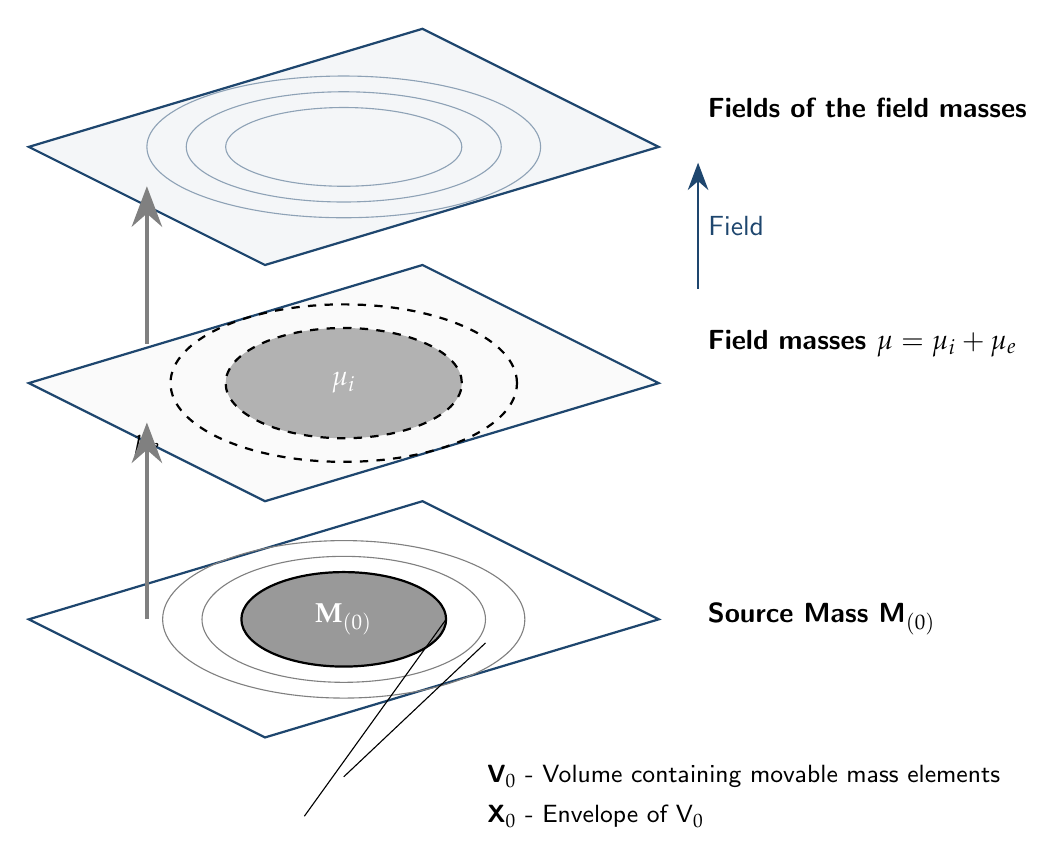
\begin{tikzpicture}[
    node distance=0.4cm,
    arrow/.style={-{Stealth[scale=1.5]}, thick, theoryblue}
]
    % --- 3D PLANES DRAWING ---
    % TOP PLANE: Fields
    \draw[thick, theoryblue, fill=theoryblue!5] (0,3) -- (5,4.5) -- (8,3) -- (3,1.5) -- cycle;
    \draw[thin, theoryblue!50] (4, 3) ellipse (1.5cm and 0.5cm);
    \draw[thin, theoryblue!50] (4, 3) ellipse (2cm and 0.7cm);
    \draw[thin, theoryblue!50] (4, 3) ellipse (2.5cm and 0.9cm);
    \node[font=\bfseries\sffamily, align=left, anchor=west] at (8.5, 3.5) {Fields of the field masses};
    
    % MIDDLE PLANE: Field masses (mu)
    \fill[theorygray!50] (0, 0) -- (5, 1.5) -- (8, 0) -- (3, -1.5) -- cycle;
    \draw[thick, theoryblue] (0, 0) -- (5, 1.5) -- (8, 0) -- (3, -1.5) -- cycle;
    
    \fill[gray!60] (4, 0) ellipse (1.5cm and 0.7cm);
    \draw[dashed, thick] (4, 0) ellipse (1.5cm and 0.7cm);
    \draw[dashed, thick] (4, 0) ellipse (2.2cm and 1.0cm); % V0 Volume mapping
    
    \node[font=\bfseries, white] at (4, 0) {$\mu_i$};
    \node[font=\bfseries] at (1.5, -0.8) {$\mu_e$};
    \node[font=\bfseries\sffamily, anchor=west] at (8.5, 0.5) {Field masses $\mu = \mu_i + \mu_e$};
    
    % BOTTOM PLANE: Mass M(0)
    \draw[thick, theoryblue, fill=white] (0, -3) -- (5, -1.5) -- (8, -3) -- (3, -4.5) -- cycle;
    
    % Cylinder for M(0)
    \fill[gray!80] (4, -3) ellipse (1.3cm and 0.6cm);
    \draw[thick] (4, -3) ellipse (1.3cm and 0.6cm);
    \node[font=\bfseries, white] at (4, -3) {M$_{(0)}$};

    \draw[thin, gray] (4, -3) ellipse (1.8cm and 0.8cm);
    \draw[thin, gray] (4, -3) ellipse (2.3cm and 1cm);
    \node[font=\bfseries\sffamily, anchor=west] at (8.5, -3) {Source Mass M$_{(0)}$};

    % Connective arrows
    \draw[arrow] (8.5, 1.2) -- (8.5, 2.8) node[midway, right, font=\sffamily] {Field};
    \draw[arrow, gray, line width=1.5pt] (1.5, -3) -- (1.5, -0.5);
    \draw[arrow, gray, line width=1.5pt] (1.5, 0.5) -- (1.5, 2.5);

    % Annotations for V0 and X0
    \draw[thin] (4, -5.0) -- (5.8, -3.3);
    \node[font=\sffamily\small, anchor=west] at (5.7, -5.0) {\textbf{V$_0$} - Volume containing movable mass elements};
    \draw[thin] (3.5, -5.5) -- (5.3, -3.0);
    \node[font=\sffamily\small, anchor=west] at (5.7, -5.5) {\textbf{X$_0$} - Envelope of V$_0$};

\end{tikzpicture}
\end{adjustbox}
\caption{The hierarchical mapping of source mass $M_{(0)}$ and the resulting internal/external field masses ($\mu_i, \mu_e$) acting as secondary sources of gravitation.}
\end{figure}

To formalize this, Heim establishes a rigorous set of mass and density definitions that differentiate between the global volume ($V$) and the localized source volume ($V_0$):

\begin{table}[htbp]
\centering
\renewcommand{\arraystretch}{1.5}
\begin{tabular}{@{}p{1.2cm} p{6cm} p{3.5cm} p{3.5cm}@{}}
\toprule
\textbf{Mass} & \textbf{Meaning} & \textbf{Global Density ($V$)} & \textbf{Density within $V_0$} \\
\midrule
\rowcolor{theoryblue!5}
$M_{(0)}$ & Source masses (without field masses) & $\displaystyle \delta_0 = \frac{M_{(0)}}{V}$ & $\displaystyle \delta_{0(0)} = \frac{M_{(0)}}{V_0}$ \\
$\mu$ & Total field mass ($= \mu_i + \mu_e$) & $\displaystyle \delta_{g\mu} = \frac{\mu}{V}$ & \\
\rowcolor{theoryblue!5}
$\mu_i$ & Internal portion of field mass in $V_0$ & & $\displaystyle \sigma_i = \frac{\mu_i}{V_0}$ \\
$\mu_e$ & External portion (only outside of $V_0$) & $\displaystyle \sigma_e = \frac{\mu_e}{V - V_0}$ & \\
\rowcolor{theorygray!30}
$M_0$ & Internal total mass ($= M_{(0)} + \mu_i$) & $\displaystyle \sigma_{g0} = \frac{M_0}{V}$ & \\
$M$ & Total mass (masses + field masses) \newline ($= \mu_e + \mu_i + M_{(0)} = \mu + M_{(0)}$) & $\displaystyle \sigma_g = \frac{M}{V}$ & \\
\bottomrule
\end{tabular}
\caption{Overview of the masses and densities defined in Gravitation Dynamics.}
\end{table}

This leads to Heim's basic starting approach, the \textbf{Extended Poisson Equation}, where the total effective mass density $\sigma$ is a function of both the source mass and its own field mass:
\begin{equation}
    \operatorname{div} \vec{G} = \frac{\sigma}{\alpha}, \quad \text{where } \sigma = \sigma(M_{(0)} + \mu_i + \mu_e)
    \label{eq:heim_poisson}
\end{equation}
where $\alpha$ is a scaling factor defined as a positive constant ($\alpha > 0$).

\subsubsection{The Triple Metric of Gravity}
Heim's most radical departure from General Relativity regarding the nature of the gravitational field is the \textbf{Triple Metric Composition}. While Einstein treats gravity as a single metric $g_{ik}$, Heim proves (Volume 1, Page 79) that the gravitational field is actually composed of three equivalent metrical partial structures:
\begin{equation}
    g_{ik}(g_{ik}^{(1)}, g_{ik}^{(2)}, g_{ik}^{(3)}) = g_{ki}^*
\end{equation}
These three partial structures correspond to the interaction of the $R_3, T,$ and $S_2$ subspaces. Heim demonstrates that gravity is the result of these three "sub-forces" superimposing. Because these structures are non-Hermitian and interact as a composite, the resulting gravitational force is \textbf{geometrically diluted}. This provides a purely structural explanation for the "Hierarchy Problem" in physics—explaining why gravity is $10^{40}$ times weaker than electromagnetism. It is not because gravity is inherently "weak," but because it is a third-order singular mapping of a much stronger $R_6$ tension.

\subsection{Derivation of the Meso-field (\texorpdfstring{$\vec{\mu}$}{mu})}

To mathematically describe a temporally variable mass distribution, Heim analyzes the total density of a system. As established, the total mass $M$ consists of the source mass $M_{(0)}$ and the field masses $\mu_i$ and $\mu_e$:
\begin{equation}
    M = M_{(0)} + \mu_i + \mu_e = \text{const}
\end{equation}

Assuming a temporally variable mass distribution with a constant total mass (due to the conservation of energy and superposition), the total time derivative of the density must be zero:
\begin{equation}
    \frac{\diff\sigma}{\diff t} = 0
\end{equation}

We expand this total derivative into its partial components (derivation after $x_1, x_2, x_3, t$):
\begin{equation}
    \frac{\diff\sigma}{\diff t} = \dot{\sigma} + \sum_{k=1}^3 \frac{\partial \sigma}{\partial x_k} \dot{x}_k = \dot{\sigma} + \sum_{k=1}^3 \frac{\partial \sigma}{\partial x_k} \frac{\diff x_k}{\diff t}
\end{equation}

Assuming there is no source of velocity (the kinetic energy remains constant, and mass elements do not accelerate), we have $\operatorname{div} \vec{v} = 0$. We can adapt this to $\sigma \operatorname{div} \vec{v} = 0$. 

Substituting $\vec{v} \cdot \operatorname{grad} \sigma$ into the expanded derivative yields:
\begin{equation}
    \dot{\sigma} + \vec{v} \cdot \operatorname{grad} \sigma = 0
\end{equation}
By extending this with the condition $\sigma \operatorname{div} \vec{v} = 0$, we arrive at the continuity equation:
\begin{equation}
    0 = \dot{\sigma} + \operatorname{div}(\sigma \vec{v}) \implies \dot{\sigma} = -\operatorname{div}(\sigma \vec{v})
    \label{eq:continuity}
\end{equation}

Simultaneously, we take the partial time derivative ($\frac{\partial}{\partial t}$) of the Extended Poisson Equation ($\alpha \operatorname{div} \vec{G} = \sigma$):
\begin{equation}
    \alpha \operatorname{div} \dot{\vec{G}} = \dot{\sigma}
    \label{eq:poisson_dot}
\end{equation}

Substituting Equation (\ref{eq:continuity}) into Equation (\ref{eq:poisson_dot}) yields:
\begin{equation}
    \alpha \operatorname{div} \dot{\vec{G}} = -\operatorname{div}(\sigma \vec{v})
\end{equation}
Rearranging this, we obtain a source-free sum:
\begin{equation}
    0 = \operatorname{div} (\alpha \dot{\vec{G}} + \sigma \vec{v})
\end{equation}

\textbf{Geometric Conclusion:} The sum of the temporal gravitation field fluctuation and the impulse density ($m\vec{v}/V$) is source-free, which is another expression of the equivalence of inertia and gravitation. 

Because the divergence of this sum is strictly zero, there must exist an auxiliary vector field (the mesofield) $\vec{\mu}(x,t)$ such that its curl equals this sum:
\begin{equation}
    b \operatorname{rot} \vec{\mu} = \alpha \dot{\vec{G}} + \sigma \vec{v}
    \label{eq:mesofield}
\end{equation}
where $b \neq 0$ is an unknown proportionality factor. 

This Meso-field $\vec{\mu}$ describes the temporal change of the gravitational field. It runs orthogonally, similarly to the electromagnetic field where $\operatorname{rot} \vec{H} = \varepsilon \dot{\vec{E}} + \kappa \vec{E}$ and $\vec{H} \perp \vec{E}$.

\subsection{The Structural Field \texorpdfstring{$\vec{f}(x)$}{f(x)} and Wave Propagation}

To understand how this dynamic gravitational field propagates through space, we apply the rotation (curl) operator to Equation (\ref{eq:mesofield}):
\begin{equation}
    b \operatorname{rot} \operatorname{rot} \vec{\mu} = \alpha \operatorname{rot} \dot{\vec{G}} + \operatorname{rot}(\sigma \vec{v})
\end{equation}

Using the vector identity $\operatorname{rot} \operatorname{rot} \vec{\mu} = \operatorname{grad} \operatorname{div} \vec{\mu} - \operatorname{div} \operatorname{grad} \vec{\mu}$, we obtain:
\begin{equation}
    b(\operatorname{grad} \operatorname{div} \vec{\mu} - \operatorname{div} \operatorname{grad} \vec{\mu}) = \alpha \operatorname{rot} \dot{\vec{G}} + \operatorname{rot}(\sigma \vec{v})
\end{equation}

Rearranging this to isolate a substitution vector $\vec{w}$:
\begin{equation}
    \vec{w} = \operatorname{grad} \operatorname{div} \vec{\mu} - \frac{\operatorname{rot}(\sigma \vec{v})}{b} = \operatorname{div} \operatorname{grad} \vec{\mu} + \frac{\alpha}{b} \operatorname{rot} \dot{\vec{G}}
\end{equation}

Heim proceeds with an assumption: The mesofield $\vec{\mu}$ spreads as a wave in space with a speed $1/a$, satisfying:
\begin{equation}
    a^2 \ddot{\vec{\mu}} = \operatorname{div} \operatorname{grad} \vec{\mu}, \quad a^2 \neq 0
\end{equation}

Substituting this into the $\vec{w}$ equation, we get:
\begin{equation}
    \vec{w} = a^2 \ddot{\vec{\mu}} + \frac{\alpha}{b} \operatorname{rot} \dot{\vec{G}}
\end{equation}
Setting $a^2 = -\alpha \beta$, the wave equation aligns into:
\begin{equation}
    \vec{w} = -\alpha \beta \ddot{\vec{\mu}} + \frac{\alpha}{b} \operatorname{rot} \dot{\vec{G}} \quad \left[ \frac{\text{kg}}{\text{m}^3 \text{ s}} \right]
\end{equation}

Heim argues that the substitution $\vec{w}$ depends on the temporal change of the differential density. Because the total mass is defined as $M(x,t) = M_{(0)} + \mu(x,t)$, and the source mass $M_{(0)}$ is constant in reference to $x$ and $t$, the time derivative of the density simplifies to $\dot{\sigma} = \dot{\sigma}_\mu$.

Heim introduces an un-dimensioned structural field $\vec{f}(x)$, which is temporally constant and describes a fundamental property of space, setting $\vec{w} = \dot{\sigma}_\mu \vec{f}(x)$. Equating the two expressions for $\vec{w}$ and rearranging yields:
\begin{equation}
    \frac{\alpha}{b} \operatorname{rot} \dot{\vec{G}} = \alpha \beta \ddot{\vec{\mu}} + \dot{\sigma}_\mu \vec{f}(x)
\end{equation}

We integrate this entire expression with respect to time ($\int \diff t$):
\begin{equation}
    \frac{\alpha}{b} \operatorname{rot} \vec{G} = \alpha \beta \dot{\vec{\mu}} + \sigma_\mu \vec{f}(x)
\end{equation}
Substituting $\sigma_\mu = \sigma - \sigma_{(0)}$, we get:
\begin{equation}
    \frac{\alpha}{b} \operatorname{rot} \vec{G} = \alpha \beta \dot{\vec{\mu}} + (\sigma - \sigma_{(0)}) \vec{f}(x)
\end{equation}

Next, we apply the divergence operator (div) to this equation. Since $\operatorname{div} \operatorname{rot} = 0$, the left side vanishes:
\begin{equation}
    0 = \alpha \operatorname{div} \beta \dot{\vec{\mu}} + \operatorname{div}((\sigma - \sigma_{(0)})\vec{f}(x))
\end{equation}

Heim introduces a final geometric assumption: The structural field $\vec{f}(x)$ runs orthogonally to the gradient of the mass density ($\vec{f}(x) \perp \operatorname{grad}(\sigma - \sigma_{(0)})$). Therefore, the dot product vanishes, yielding the final coupled summary of Gravitodynamics:

\begin{tcolorbox}[colback=white, colframe=theoryblue, title=\textbf{Summary of Dynamic Gravitation Law}]
\begin{align}
    \operatorname{rot} \vec{G} &\sim \beta \dot{\vec{\mu}} + \frac{\sigma - \sigma_{(0)}}{\alpha} \vec{f}(x) \label{eq:grav_summary1} \\
    \alpha \beta \operatorname{div} \dot{\vec{\mu}} &= -(\sigma - \sigma_{(0)}) \operatorname{div} \vec{f} \label{eq:grav_summary2}
\end{align}
\textit{Where $\beta = \text{const} \neq 0$.}
\end{tcolorbox}

\subsubsection{The Gravitational Lorentz Force}
In classical electrodynamics, a moving charge $q$ is acted upon by the Lorentz force: $\vec{F}_E = q(\vec{E} + \vec{v} \times \vec{B})$. Because Heim's dynamic gravitation law exhibits perfect structural symmetry with Maxwell's equations, a mass $m$ moving with velocity $\vec{v}$ through a dynamic gravitational field experiences an analogous \textbf{Gravito-Lorentz Force}:
\begin{equation}
    \vec{F}_G = m \left( \vec{G} + \vec{v} \times \vec{\mu} \right)
\end{equation}

Under normal terrestrial conditions, the velocity of mass is so small relative to the gravitational propagation speed ($\omega$) that the cross product $\vec{v} \times \vec{\mu}$ approaches zero, leaving only Newton's static weight ($\vec{F} = m\vec{G}$). However, in astrophysical scenarios with rapidly spinning, super-massive objects (like pulsars or black holes), this gravitomagnetic mesofield ($\vec{\mu}$) becomes a dominant physical force, responsible for relativistic frame-dragging and axial jet formation.

\subsection{The Propagation Speed and the Auxiliary Spacetimes}

To estimate the propagation speed of this dynamic gravity, Heim evaluates the equations in an area free from static and dynamic sources ($v = 0$, $\sigma \approx \sigma_{(0)}$). Under these conditions, the fundamental dynamic equations simplify to:
\begin{equation}
    \operatorname{rot}\vec{\mu} = \alpha\dot{\vec{G}} \quad \text{and} \quad \operatorname{rot}\vec{G} = \beta\dot{\vec{\mu}}
\end{equation}

By cross-substituting their time derivatives and spatial rotations, Heim derives the \textbf{General Propagation Equation for Gravitation} for the potential field $\vec{p} \hat{=} (\vec{G}, \vec{\mu})$:
\begin{equation}
    \operatorname{divgrad}\vec{p} + \frac{1}{\omega^2} \frac{\partial^2 \vec{p}}{\partial t^2} = \vec{0}, \quad \text{where } \omega^2 = \frac{1}{\alpha |\beta|}, \quad 0 < \omega < \infty
\end{equation}

Here, $\omega$ is the finite propagation speed of gravitational disturbances. However, a critical mathematical bifurcation occurs depending on the sign of the constant $\beta$:

\begin{enumerate}
    \item \textbf{Possibility 1 ($\beta < 0$):} This results in an imaginary time coordinate $x_{-4} = \iu \omega t$. This yields a transversal wave equation for "gravitational radiation." Heim rejects this as the primary framework because macroscopic transversal gravitational waves were not empirically observed at the time.
    \item \textbf{Possibility 2 ($\beta > 0$):} This results in a real time coordinate $x_{+4} = \omega t$. This yields a four-dimensional potential equation describing the propagation of a field disturbance. Heim accepts this because tidal effects (temporal potential fluctuations) between planets are observable.
\end{enumerate}

\subsection{The Dual Spacetime Matrices and Commutativity}

By asserting $\beta > 0$, Heim splits the mathematical description of the universe into two auxiliary, tangent spacetimes. This resolves the mathematical clash between electromagnetism and gravitation:

\begin{itemize}
    \item \textbf{Einstein's Electromagnetic World ($R_{-4}$):} Governed by imaginary light-time $x_{-4} = \iu c t$. Transformation occurs via the Unitary Lorentz Matrix $\hat{\mathbf{A}}_-$.
    \item \textbf{Heim's Gravitation World ($R_{+4}$):} Governed by real gravity-time $x_{+4} = \omega t$. Transformation occurs via the Orthogonal Lorentz Matrix $\hat{\mathbf{A}}_+$.
\end{itemize}

A unified field tensor $\mathbf{M}_{km}(R_4)$ must be invariant against the general Lorentz transformation in true spacetime, which is the product of these two matrices:
\begin{equation}
    \hat{\mathbf{B}} = \hat{\mathbf{A}}_+ \hat{\mathbf{A}}_-
\end{equation}

To prove that the propagation of gravity ($\omega$) does not interfere with the constancy of the speed of light ($c$), Heim analyzed the special case of a constant movement $v$ along the $x_1$ axis. Because $\hat{\mathbf{A}}_+$ is an orthogonal rotation matrix and $\hat{\mathbf{A}}_-$ operates on an imaginary axis, their commutator evaluates to zero ($[\hat{\mathbf{A}}_+, \hat{\mathbf{A}}_-] = 0$). 

\textbf{Physical Implication:} The multiplication is perfectly commutative. This proves mathematically that the speed of gravitational propagation ($\omega$) acts completely independently of the speed of light limit ($c$). In standard relativistic measurements, the gravitational coordinate $x_{+4}$ appears merely as a minuscule scalar correction factor ($\approx 1$) acting on the Minkowskian background. Therefore, the failure to measure $\omega$ directly does not invalidate the theory; the geometry naturally hides the gravitational time coordinate behind the dominant electromagnetic metric.

\section{The Reputation of Unified Field Theory}

Let's take a look at the reputation surrounding unified field theory during that era.

\begin{itemize}
    \item \textbf{Michio Kaku:} ``Einstein believed that his unified field theory should be able to automatically explain key aspects of quantum mechanics as a by-product. He believed that atoms only appeared as solutions to his geometric theories of gravity and light. He became increasingly obsessed with purely mathematical concepts such as `twisted' geometry—bizarre mathematical structures that had no physical meaning.''
    \item \textbf{Lee Smolin:} ``In the 1940s, Einstein and a few others were searching for a unified field theory, but it was met with almost complete derision.''
\end{itemize}

\subsection{The Voices of the Contemporaries}
\begin{description}
    \item[Oppenheimer:] ``Einstein's research is useless.''
    \item[Dyson:] ``I read a copy of Einstein's latest paper last night and decided it was hopeless. I canceled the meeting.''
    \item[Bohr:] ``Albert became an alchemist.''
    \item[Schrödinger:] (For some reason, angry): ``My method is far superior! Let me explain. Albert is a foolish old man!''
\end{description}

They were all terrible. However, this was the era of the great business boom—quantum mechanics, atomic bombs, nuclear power, and quantum chemistry. In the midst of the development of 20th-century civilization, a ``unified theory of electromagnetism and gravity,'' a quintessential classical theory, was treated as an antique.

\subsection{Feynman on the "Children's Dream"}

What did Richard Feynman say in his \textit{Lectures on Gravitation}?

\begin{fancyquote}
    Einstein's theory of gravity... established a beautiful relationship linking gravitational phenomena with the geometry of space. This was an inspiring idea. The apparent similarities between gravity and the electric force, in that they both obey the inverse square law, for example, are understandable to every child, and every one of these `children,' when he grew up, dreamed of finding a way to geometrize electromagnetism.
\end{fancyquote}

\begin{fancyquote}
    Thus, a generation of physicists worked to create a so-called unified field theory that would unify gravity and electromagnetism into a single one. None of these unified field theories were successful... Most of them are mathematical games, invented by mathematically-minded people with little knowledge of physics, and most of them are incomprehensible. Einstein himself worked on this... but nevertheless, there is no successful unified field theory that combines gravity and electrodynamics.
\end{fancyquote}

Feynman argued that such success would have been short-lived, as physics now deals with much more: mesons, K-mesons, neutrinos, and over 30 other particles. Unifying only EM and Gravity would not have been a major achievement given the complexity of the subatomic world.

\begin{reflectionbox}[title={Response to Feynman}]
\textbf{Note's and Response:} I understand what the ``big boys'' are saying, but I think it's fine to just go with the dreams of the ``kids'' here, including elementary particles. We already have a verifiable mass formula (or something that looks like a pinhole).
\end{reflectionbox}

\subsection{Appendix: The Asymmetric Metric}

Why does it have to be this way? Since Einstein discovered the theory of gravitational fields in 1915, there have been constant attempts to generalize it to explain electromagnetic fields. Since the latter are in a space described by a second-order antisymmetric tensor, the idea is to make the metric \textbf{asymmetric}, where the antisymmetric part must have something to do with electromagnetism. However, this plan poses certain difficulties.


% ==============================================================================
\section{Detour: Part 2 — Twisted Geometry and the Scholarship Anecdote}
% ==============================================================================

I'm still making detours. Something that caught my attention in the last post was this:

\begin{fancyquote}
    He [Einstein] gradually became obsessed with purely mathematical concepts such as `twisted' geometry — bizarre mathematical structures that had no physical meaning.
\end{fancyquote}

Speaking of bizarre mathematical structures, I personally think superstring theory is even more bizarre. Incidentally, this concept apparently originated in 1922 with the French mathematician \textbf{Élie Cartan}.

\subsection{Cartan and the Generalization of Curvature}
In his notes, \textit{``Sur une généralisation de la notion de courbure de Riemann et les espaces à torsion''} (A generalization of the concept of Riemann curvature and torsion space), Cartan showed how, in the Einstein universe ($ds^2$), the energy tensor attached to each volume element can be defined geometrically.

Ultimately, Cartan's theory suggests that \textbf{energy can be described geometrically as the ``rotation = twist'' (torsion) of space}. This is a broader concept than the curvature found in General Relativity, adding a degree of freedom for twisting.

\begin{itemize}
    \item \textbf{Note's and Note:} Does this mean there are actually extra degrees of freedom in Lorentz transformations? If we only need to preserve four-vectors, we could potentially ``twist'' them. However, frames with torsion aren't typically called inertial frames. I'll keep my fantasies to a minimum for now.
\end{itemize}

\subsection{Heim's 1952 Scholarship Encounter}

Let's look back at Burkhard Heim's own recollections:

\begin{fancyquote}
    \textbf{Heim:} ``In 1952, I wanted to take an exam on unified field theory for my scholarship. None of my professors wanted to administer the exam, because none of them could. I was in a bind—the pension office had recommended me—so I went to see \textbf{Carl Friedrich von Weizsäcker}.''
\end{fancyquote}

Von Weizsäcker was remarkably candid:

\begin{fancyquote}
    \textbf{Von Weizsäcker:} ``I can't do it either, but I've always wanted to learn it. So tell me about it! Then I'll give it credit!''
\end{fancyquote}

Heim argued that unification could not be done the way Einstein suggested. He pointed out that if you apply the metric tensor asymmetrically (as Einstein did), the anti-Hermitian parts cancel out in the line element, leaving only the standard Riemannian metric.

\begin{fancyquote}
    \textbf{Von Weizsäcker:} ``Yes, it's known. \textbf{Wolfgang Pauli} already said so. That's what Pauli told me in a conversation a few days ago.''
\end{fancyquote}

Pauli was notoriously dismissive of unified field theories, famously stating:
\begin{center}
    \textit{``What God has put asunder, let no one put together.''}
\end{center}

To which Heim reportedly replied with somewhat impertinent confidence:
\begin{center}
    \textit{``Asunder? We only know that Einstein placed separate fields and sources.''}
\end{center}

Student Heim essentially taught unified field theory to Professor von Weizsäcker to secure his scholarship. Meanwhile, Einstein (in 1946) was still active, noting that ``formally, the Hermitian restriction is unnecessary.'' All these legends were debating while Japan was still in its post-war reconstruction.

\subsection{The Worldview of Burkhard Heim}

In a 2001 memorial article for Heim, there is a powerful photo from 1969 showing him writing mathematical formulas on a blackboard using his disabled arm (a result of a laboratory explosion during the war).

The blackboard displayed theoretical formulas for:
\begin{itemize}
    \item The \textbf{charge and mass} of the electron.
    \item The \textbf{fine structure constant} ($\alpha$).
\end{itemize}

This story of his interaction with von Weizsäcker can be found in the document \textit{``Burkhard Heim's New Worldview''} (English PDF, around page 20).

\begin{sectionrefs}
    \item \href{https://en.wikipedia.org/wiki/%C3%89lie_Cartan}{Élie Cartan}: On the generalization of Riemann curvature and torsion space (geometric definition of the energy tensor).
    \item \href{http://archiv.mufon-ces.org/text/deutsch/heim.htm}{Memorial article for Burkhard Heim (2001)}: Source for the Weizsäcker/Pauli conversation.
    \item \href{http://heim-theory.com/?page_id=161}{Burkhard Heim's New Worldview}: Source for the Weizsäcker anecdote (p. 20).
    \item \href{https://en.wikipedia.org/wiki/Wolfgang_Pauli}{Wolfgang Pauli}: Context for the statement, "What God has put asunder..."
\end{sectionrefs}

\hr

\subsection*{In-Depth: The Geometry of the Retort}
\addcontentsline{toc}{subsection}{In-Depth: The Geometry of the Retort}

Heim's confidence during the 1952 encounter with von Weizsäcker was rooted in his understanding of **Cartan's Torsion**. In 1922, Élie Cartan generalized Riemann curvature by introducing the torsion tensor $S_{ij}^k$. This allowed for a "twist" in the manifold:

\begin{equation}
    \Gamma_{ij}^k - \Gamma_{ji}^k = 2 S_{ij}^k
\end{equation}

Where $\Gamma_{ij}^k$ are the affine connections. In standard General Relativity, the connections are symmetric (Levi-Civita), meaning torsion is zero. Heim recognized that Einstein's attempt to geometrize matter was failing because it stayed within a "torsion-free" framework. 

When Heim told von Weizsäcker that Einstein had "placed" fields and sources separately, he was referring to the right-hand side of the field equations:
\begin{equation}
    G_{ik} = \kappa T_{ik}
\end{equation}
The left side ($G_{ik}$) is the "Marble" (pure geometry), while the right side ($T_{ik}$) is the "Wood" (phenomenological matter). Heim’s worldview, which he would present at MBB 24 years later, was to prove that $T_{ik}$ is itself a manifestation of the "twists" in a 6-dimensional quantized geometry, thereby completing the marble building Einstein left unfinished.
% ==============================================================================
% ==============================================================================
\section{MBB Lecture Part 2: Invariant Theory of Gravity}
% ==============================================================================
\textit{MBB Lectures, Chapter 3, pp. 22-29}

Now, let's get back to the main topic. As a note on the translation, I have used both DeepL and Google as references to ensure the nuances of the original German are captured. This section focuses on the formalization of gravitational phenomena.

\subsection{Formulation of an Invariant Theory of Gravity}
\textit{Volume 1, Chapter 1-2}

Unfortunately, Newton's law of gravity certainly doesn't apply in the immediate vicinity of elementary particles, so very little is known about this gravitational phenomenon. Also, we don't know how the gravitational field works at that scale! However, we can still draw some conclusions. For example, we can say that gravity is clearly a state different from nothingness.

For anything to exist or be created, energy is required. Energy and inertial mass can be responsible for gravitational effects, but they are equivalent ($E=mc^2$). On the other hand, the gravitational field itself seems to have additive properties, relative to the field's inertia. Frankly, I find it difficult to assume that matter as a whole creates a gravitational field while its final components should not. If there are quanta of matter, these quanta seem to define at least a fundamental gravitational field.


Now, I don't know if the gravitational field is a quantum field, but for the sake of argument, let's assume that it is. The \textbf{uncertainty principle} generally applies to quantum fields, meaning certain conjugate pairs cannot be measured simultaneously. For example, there is a fundamental uncertainty in position/momentum and energy/time, at least as large as Planck's quantum of action ($h$).

If we assume there is an interaction force connecting two things, this uncertainty relation applies. If we use the bare gravitational effect instead of this interaction force, it seems difficult to imagine that we can suddenly accurately measure both conjugate attributes. This idea comes from \textbf{Bondi}. I still don't know how this quantization works, but I think we have to assume that gravity is also a quantized field.

\subsubsection{Dynamic Gravitational Fields}

Without going into too much detail about microscopic dimensions yet, it seems reasonable to think more concretely about the phenomenon of gravity. Although we know very little, we can incorporate Newton's law of gravity into a Poisson version of the source field. We have a field vector $\vec{G}$ (acceleration). In the static case, it is the gradient of a scalar potential:
\begin{equation}
    \vec{G} = -\nabla \Phi
\end{equation}
The divergence of this field vector is proportional to the mass density of the field source.

What happens if we introduce temporal variations? We start with a mass distribution that is not smooth, but inhomogeneous or anisotropic and changes over time. This results in a time partial derivative of the mass density. During this time variation, we assume no matter leaves a specific closed region surrounding this matter. Next, we consider the gravitational field outside the region.

% --- DIAGRAM REPLACEMENT FOR MBBfig04.png ---
\begin{center}
    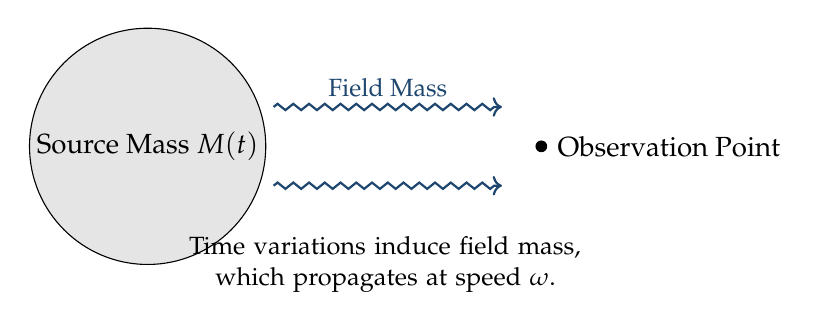
\begin{tikzpicture}
        % Big mass circle
        \draw[fill=gray!20] (0,0) circle (1.5cm);
        \node at (0,0) {Source Mass $M(t)$};
        
        % Distant point
        \node[circle, fill=black, inner sep=1.5pt, label=right:Observation Point] (P) at (5,0) {};
        
        % Field lines indicating propagation
        \draw[->, thick, theoryblue, wavy] (1.6, 0.5) -- node[above, font=\small] {Field Mass} (4.5, 0.5);
        \draw[->, thick, theoryblue, wavy] (1.6, -0.5) -- (4.5, -0.5);
        
        \node[text width=6cm, align=center, font=\small] at (3, -1.5) {Time variations induce field mass, which propagates at speed $\omega$.};
    \end{tikzpicture}
    \captionof{figure}{Dynamic gravity: The field itself possesses mass.}
\end{center}

In this way, we can extend Newton's law to account for the \textbf{mass of the field} itself, provided such time variations occur. This means that between our observation point and the source mass, there is also a gravitational field mass, which can also induce gravity. This leads us to the conclusion that gravitational field disturbances propagate at a constant speed $\omega$, which is neither zero nor infinite.

Is this speed $\omega$ the speed of light $c$? It could be, but I think we should leave the question open for now and not commit to speculation from the start.

\subsection{The Auxiliary Spacetimes \texorpdfstring{$R_{-4}$}{R-4} and \texorpdfstring{$R_{+4}$}{R+4}}

Leaving the propagation speed $\omega$ open, it is best to describe the time-varying gravitational field in real space-time. Interestingly, I do not use ordinary Minkowski space here, but rather real-time coordinates that reflect the temporal behavior of gravitational fields.

\begin{enumerate}
    \item \textbf{Electromagnetic Reality (Space $R_{-4}$):} Minkowski space with imaginary time coordinates $x_4 = ict$. This uses a unitary transformation matrix $\hat{A}_{-}$.
    \item \textbf{Gravitational Reality (Space $R_{+4}$):} A space with real-time coordinates $x_4 = \omega t$. This uses an orthogonal transformation matrix $\hat{A}_{+}$.
\end{enumerate}

(I generally refer to matrices that have orthogonal properties over real fields as ``orthogonal.'' When elements are complex, I call them ``unitary.'')

% --- DIAGRAM REPLACEMENT FOR MBBfig05.png ---
\begin{center}
    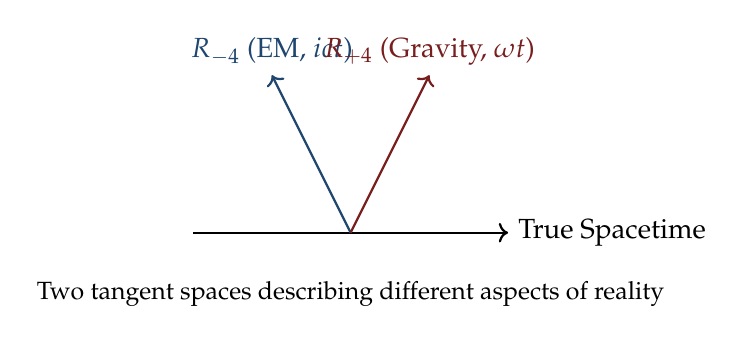
\begin{tikzpicture}
        \draw[thick, ->] (0,0) -- (4,0) node[right] {True Spacetime};
        
        \draw[thick, theoryblue, ->] (2,0) -- (1,2) node[above] {$R_{-4}$ (EM, $ict$)};
        \draw[thick, theoryred, ->] (2,0) -- (3,2) node[above] {$R_{+4}$ (Gravity, $\omega t$)};
        
        \node[below, font=\small] at (2,-0.5) {Two tangent spaces describing different aspects of reality};
    \end{tikzpicture}
    \captionof{figure}{Unified Field Description via tangent spacetimes.}
\end{center}

These two auxiliary structures appear to me to be nothing more than \textbf{tangent spacetimes} of true spacetime. The real world resembles neither alone; in the real world, there are both electromagnetic and gravitational effects.

Multiplying the two Lorentz matrices—the orthogonal matrix of the gravitational world and the unitary matrix of electromagnetic relativity—shows that the commutator is zero:
\begin{equation}
    [\hat{A}_{+}, \hat{A}_{-}] = 0
\end{equation}
This confirms the multiplication is commutative. It becomes clear that the propagation speed of gravitational field disturbances ($\omega$) cannot affect the speed limit of light ($c$) for matter in a substantial way. Any deviation is practically immeasurable with today's technology.

\hr

\begin{reflectionbox}[title={Notes and Reflections: The Brain Complains}]
``What are you talking about, Professor Heim?'' Chapter 3 is quite difficult. Heim uses unique symbols like $\hat{A}_{+}, \hat{A}_{-}, R_{+4}, R_{-4}$ which are dazzling. My brain is complaining:
\begin{fancyquote}
    \textit{Wait a minute! Gravity is dealt with in General Relativity, not here. Gravity is an apparent force in curved space. Its propagation speed is $c$! Stop!}
\end{fancyquote}
But I'll hold off. The route everyone is taught to be correct leads to a dead end with an incomplete unified theory, so maybe it's okay to see where this path goes.
\end{reflectionbox}

\subsection{The Mesofield \texorpdfstring{$\mu$}{mu} (Gravitomagnetism)}

To follow the details, one needs to understand the derivation of $\mu$, the ``mesofield,'' which is the gravitational equivalent of the magnetic field.

\textbf{Logic:} The time change of the gravitational field should be balanced with the mass density flow rate, so we assume the divergence is zero:
\begin{equation}
    \nabla \cdot \left( \alpha \frac{\partial \vec{G}}{\partial t} + \sigma \vec{\nu} \right) = 0
\end{equation}
From here, we can define $\vec{\mu}$ like the vector potential of a magnetic field:
\begin{equation}
    b \nabla \times \vec{\mu} = \alpha \frac{\partial \vec{G}}{\partial t} + \sigma \vec{\nu}
\end{equation}
where $\alpha$ and $b$ are proportionality constants. This allows for the derivation of wave equations for $\vec{G}$ and $\vec{\mu}$.

\bigskip
\textbf{Questions for this Section:}
\begin{itemize}
    \item[\fbox{?}] \textbf{Q.01:} What is the basis for saying that the gravitational field alone is simply a Euclidean metric?
    \item[\fbox{?}] \textbf{Q.02:} Two tangent spacetimes? What does that mean for the dimensionality of the ``true'' spacetime?
\end{itemize}

\begin{sectionrefs}
    \item \href{https://www.engon.de/protosimplex/index_e.htm}{Protosimplex (English Downloads)}.
    \item \href{https://en.wikipedia.org/wiki/Hermann_Bondi}{Hermann Bondi}: Referenced for the concept of gravitational field quantization and uncertainty.
    \item \href{https://en.wikipedia.org/wiki/Gravitoelectromagnetism}{Gravitoelectromagnetism (GEM)}: Context for the mesofield ($\mu$) and the extension of Newton's law to include field mass.
\end{sectionrefs}

\hr

\subsection*{In-Depth: The Formalism of Gravitation Dynamics (Map I-2)}
\addcontentsline{toc}{subsection}{In-Depth: The Formalism of Gravitation Dynamics}

To formalize the transition from Newton's static law to a dynamic field theory, Heim utilizes a Poisson-like approach for the gravitational field vector $\vec{G}$ (acceleration). The core of this derivation, as detailed in the Map I-2 supplements, relies on the redefinition of mass density and the introduction of the Meso-field.

\subsubsection*{1. Redefining the Source $\sigma$}
In Heim's theory, the total mass density $\sigma$ must include not only the source masses but also the energy-equivalent field masses. If we define $M_{(0)}$ as source mass, $\mu_i$ as internal field mass, and $\mu_e$ as external field mass, the total density is:
\begin{equation}
    \sigma = \sigma(M_{(0)} + \mu_i + \mu_e)
\end{equation}
This leads to the modified Poisson equation:
\begin{equation}
    \operatorname{div} \vec{G} = \frac{\sigma}{\alpha} \quad (\alpha = \text{scaling factor})
\tag{I-2.1}
\end{equation}

\subsubsection*{2. The Meso-field and Vectorial Orthogonality}
Consider a temporally variable mass distribution where the total density remains constant ($\frac{d\sigma}{dt} = 0$). By applying the continuity equation $\dot{\sigma} = -\operatorname{div}(\sigma \vec{\nu})$, where $\vec{\nu}$ is the velocity field, and substituting into the time derivative of Equation (I-2.1), we derive the source-free sum:
\begin{equation}
    \operatorname{div}(\alpha \dot{\vec{G}} + \sigma \vec{\nu}) = 0
\end{equation}
Since this sum is divergence-free, it must be the rotation of an auxiliary vector field, which Heim identifies as the \textbf{Mesofield} $\vec{\mu}$.

\begin{tcolorbox}[colback=white, colframe=theoryblue, title=\textbf{The Dynamic Gravitation Law}]
The relationship between the gravitational acceleration $\vec{G}$ and the gravito-magnetic mesofield $\vec{\mu}$ is defined as:
\begin{align}
    \operatorname{div} \vec{G} &= \frac{\sigma}{\alpha} \\
    b \operatorname{rot} \vec{\mu} &= \alpha \dot{\vec{G}} + \sigma \vec{\nu}, \quad (b \neq 0)
\end{align}
\textbf{Constraint:} The field $\vec{\mu}$ runs orthogonally to the induction sum: $\vec{\mu} \perp (\alpha \dot{\vec{G}} + \sigma \vec{\nu})$.
\end{tcolorbox}

\subsubsection*{3. The Selection of Real Time for Gravity ($\beta > 0$)}
Defining the field potential as $\vec{p} \hat{=} (\vec{G}, \vec{\mu})$, the wave propagation in source-free space follows:
\begin{equation}
    \operatorname{div} \operatorname{grad} \vec{p} + \alpha \beta \ddot{\vec{p}} = \vec{0}, \quad \omega^2 = \frac{1}{\alpha |\beta|}
\end{equation}
Heim identifies two mathematical possibilities for the coordinate $x_4$:
\begin{itemize}
    \item \textbf{Possibility 1 ($\beta < 0$):} $x_4 = i \omega t$ (Transversal wave/Radiation).
    \item \textbf{Possibility 2 ($\beta > 0$):} $x_4 = \omega t$ (Four-dimensional potential/Real-time propagation).
\end{itemize}
Heim selects \textbf{Possibility 2}, as tidal potential fluctuations between planets are empirically observed, whereas macroscopic transversal gravitational radiation remains elusive in the Newtonian approximation.

\subsubsection*{4. The Commutativity of Dual Spacetimes}
The "True Spacetime" is the intersection of the electromagnetic manifold $R_{-4}$ and the gravitational manifold $R_{+4}$.
\begin{itemize}
    \item \textbf{$R_{-4}$ (Einstein):} Imaginary light-time $x_4 = ict$, Unitary matrix $\hat{\mathbf{A}}_{-}$.
    \item \textbf{$R_{+4}$ (Heim):} Real gravity-time $x_4 = \omega t$, Orthogonal matrix $\hat{\mathbf{A}}_{+}$.
\end{itemize}
Heim proves that the commutator of these transformation matrices is zero:
\begin{equation}
    [\hat{\mathbf{A}}_{+}, \hat{\mathbf{A}}_{-}] = 0
\end{equation}
This confirms that the propagation speed of gravity ($\omega$) acts independently of the speed of light ($c$), and that gravitational measurements appear only as correction factors of magnitude $\approx 1$ in the standard Lorentz matrix. 
% ============================================================================== 
% ==============================================================================
% CHAPTER 3: THE NON-HERMITIAN UNIFIED FIELD AND QUANTIZATION
% ==============================================================================

\section{The Dual Views of Spacetime: Geometrical vs. Physical}
\label{sec:non_hermitian}

\textit{References: MBB Lecture Transcript; Map I-3 (Derivation of the non-hermitian structure of $R_4$)}

Having established the dynamical laws of gravitation and the necessity of a 6-dimensional manifold, Heim sought to unify the gravitational and electromagnetic fields into a single mathematical structure within our observable 4D space-time ($R_4$). To achieve this, he mapped the problem from two simultaneously converging perspectives: the \textbf{Geometrical View} (Einstein’s "Marble") and the \textbf{Physical View} (Einstein’s "Wood").

\subsection{The Geometrical View: From Empty Space to Cartan Geometry}

In a completely empty $R_4$, points are homogeneously distributed. There are no distinguishable event structures, meaning no physical matter exists. Consequently, the energy-momentum tensor $T_{ik}$ does not exist. 

However, in a \textbf{Non-Empty $R_4$}, the presence of a Material Field Quantum ($M_q$) fundamentally disrupts this homogeneity. Each of the $n \ge 4$ interactions of an $M_q$ produces a partial event structure defined by its respective geodetic coordinate system:
\begin{equation}
    \vec{\xi}_p^{(j)} = \vec{\xi}_1^{(j)} \dots \vec{\xi}_4^{(j)} = f(x_1 \dots x_4) \quad \text{for } j = 1 \dots n \text{ interactions}
\end{equation}

Heim divides these interactions into two groups based on gauge invariance (\textit{Eichinvarianz}):
\begin{itemize}
    \item $m$ interactions are \textbf{non-eichvariant} (associated with gravitation). They generate the vector sum $d\vec{z}_p^+ = \sum_{j=1}^m d\vec{\xi}_p^{(j)}$.
    \item $n-m$ interactions are \textbf{eichvariant} (associated with electromagnetism). They generate the vector sum $d\vec{z}_p^- = \sum_{j=m+1}^n d\vec{\xi}_p^{(j)}$.
\end{itemize}

The resulting vectorial line element for the total distance in this space is the sum of these two partial vectors: $d\vec{s}_{\pm} = d\vec{s}_+ + d\vec{s}_-$.

\subsubsection{Investigation of the Hermite Operator and the Metric Split}

To evaluate the metric scalar $ds^2$, Heim applies the Hermite operator. Using the relation $d\vec{z}^* = \vec{z}_{,k}^* dx^k$, the quadratic form expands into three distinct operational parts:
\begin{equation}
    ds^2 = \left(g_{ik}^{(1)} + g_{ik}^{(2)} + g_{ik}^{(3)}\right) dx^i dx^k
\end{equation}

Because standard Riemannian geometry is insufficient to hold the $M_q$ interactions, the metric tensor is fundamentally forced into a \textbf{Cartan Geometry} with torsion. This explicitly splits the metric $g_{ik}$ into a symmetric (Hermitian) and an antisymmetric (Anti-Hermitian) component:
\begin{equation}
    g_{ik} = g_{ik}^{(S)} + ig_{ik}^{(A)}
\end{equation}

\textbf{The Asymmetry Breakdown:}
\begin{itemize}
    \item \textbf{$g_{ik}^{(S)}$ (Hermitian):} Arises from purely gravitational interactions ($g_{ik}^{(1)}$) and purely electromagnetic interactions ($g_{ik}^{(3)}$). It is strictly symmetric ($g_{ik} = g_{ki}^*$).
    \item \textbf{$g_{ik}^{(A)}$ (Anti-Hermitian):} Arises from the cross-term interaction ($g_{ik}^{(2)}$) between gravity and electromagnetism. It is explicitly asymmetric ($g_{ik} \neq g_{ki}^*$).
\end{itemize}

\begin{tcolorbox}[colback=white, colframe=theorygray, title=\textbf{Einstein's "Wood vs. Marble" Dilemma Resolved}]
Einstein famously complained that General Relativity was a building with one wing made of fine marble (pure geometry) and the other made of cheap wood (phenomenological mass added by hand). Heim solves this by bringing matter \textit{into} the geometry via the anti-Hermitian split.

\vspace{0.5em}
\begin{tabular}{p{7cm} | p{7cm}}
\textbf{Standard General Relativity} & \textbf{Heim Unified Field Theory} \\
\midrule
$G_{ik} = \kappa T_{ik}$ & $\hat{R}_{ik} - \frac{1}{2}\hat{g}_{ik}\hat{R} \sim \hat{T}_{ik}$ \\
\textit{Symmetric Geometry = External Wood} & \textit{Non-Hermitian Geometry = Unified Field} \\
\end{tabular}
\end{tcolorbox}

While the anti-Hermitian components vanish in the simple scalar distance calculation ($ds^2$), they persist in the affine connections ($\Gamma$) and curvature tensors ($R_{ik}$), representing the physical force fields.

\subsubsection{Splitting into Hermitian and Anti-Hermitian Parts}

Because $g_{ik}^{(2)} \neq 0$, standard Riemannian geometry is insufficient. The presence of $M_q$ forces the metric into a \textbf{Cartan Geometry} with torsion. This fundamentally splits every aspect of the geometric structure tensor into a Hermitian (symmetric) portion and an anti-Hermitian (asymmetric) portion.

\begin{table}[htbp]
\centering
\renewcommand{\arraystretch}{1.6}
\begin{tabular}{lll}
\toprule
\textbf{Geometric Property} & \textbf{Hermitian Part ($+$)} & \textbf{Anti-Hermitian Part ($-$)} \\
\midrule
\rowcolor{theoryblue!5}
\textbf{Fundamental Tensor} & $g_{ik} = g_{ik}^+$ & $+ \; g_{ik}^-$ \quad \textit{(where $g_{ik}^- = -g_{ki}^{-*}$)} \\
\textbf{Metric} & $ds^2 = g_{ik}^+ dx^i dx^k$ & $+ \; 0$ \quad \textit{(vanishes in scalar distance)} \\
\rowcolor{theoryblue!5}
\textbf{Christoffel Symbols} & $\Gamma_{km}^i = \Gamma_{(+)km}^i$ & $+ \; \Gamma_{(-)km}^i$ \\
\textbf{Curvature Tensor} & $R_{kmp}^i = R_{(+)kmp}^i$ & $+ \; R_{(-)kmp}^i$ \\
\rowcolor{theoryblue!5}
\textbf{Ricci Tensor} & $R_{km} = R_{(+)kmp}^p$ & $+ \; R_{(-)kmp}^p$ \\
\textbf{Scalar Curvature} & $R = R_{km}^+ g^{mk}_+$ & $+ \; 0$ \\
\bottomrule
\end{tabular}
\caption{The splitting of standard Riemannian geometry into Cartan geometry. While the anti-Hermitian components vanish in the simple distance calculation ($ds^2$), they persist in the affine connections ($\Gamma$) and curvature tensors, representing the physical fields.}
\end{table}
\subsubsection{The Physical View: Unifying the Field Tensors}

From the phenomenological side, Heim examines the Lorentz transformations operating within the dual spacetimes established in Chapter 2. 

\begin{itemize}
    \item \textbf{Einstein's Domain:} The Electromagnetic field operates in imaginary space-time $R_{-4}$ ($x_{-4} = ict$). It is governed by the electromagnetic Lorentz transformation $\hat{\mathbf{A}}_-$ and the electromagnetic field tensor $\mathbf{F}_{km}(R_{-4})$.
    \item \textbf{Heim's Domain:} The Gravitational field operates in real space-time $R_{+4}$ ($x_{+4} = \omega t$, if $\beta > 0$). It is governed by the gravitational Lorentz transformation $\hat{\mathbf{A}}_+$ and the gravitational field tensor $\mathbf{G}_{km}(R_{+4})$.
\end{itemize}

To combine these phenomena, Heim defines a \textbf{Uniform Field Tensor} $\mathbf{M}_{km}(R_4)$ in Minkowski space ($x_4 = ict$). This unified tensor must strictly maintain invariance against the General Lorentz transformation ($\hat{\mathbf{B}} = \hat{\mathbf{A}}_+ \hat{\mathbf{A}}_-$). 

By performing an iteration on this field tensor—specifically, tensorial multiplication of $\mathbf{M}_{km}$ with itself and taking the trace of the spectral matrix—Heim derives the \textbf{Uniform Energy-Impulse Density Tensor} ($T_{ik}$), also known as the phenomenological matter tensor:
\begin{equation}
    T_{ik} = \sum_{m=1}^4 M_{im} M_{mk}
\end{equation}

Because the interaction of gravity and electromagnetism fundamentally twists the geometry, this physical matter tensor $T_{ik}$ is strictly non-Hermitian ($T_{ik} \neq T_{ki}^*$). It naturally splits into a Hermitian (symmetric) part $T_{ik}^+$ representing pure gravity, and an anti-Hermitian (asymmetric) part $T_{ik}^-$ representing the electromagnetic field. In the purely electromagnetic case, this is written as $T_{ik}^{(E)} = W_{ik} + \Phi_{ik}$.

\subsubsection{The Dual Convergence to the Equivalence Thesis}

The core brilliance of Heim's derivation is demonstrating that the purely mathematical properties of the geometry (the "Marble") perfectly mirror the phenomenological properties of the physical fields (the "Wood"). The theories converge from two separate paths:

\begin{enumerate}
    \item \textbf{From the Geometrical View:} An empty $R_4$ consists of homogeneously distributed points $(x_1 \dots x_4)$, meaning no distinguishable event structures (and no $T_{ik}$) exist. However, in a non-empty $R_4$, each of the $n \ge 4$ interactions of a Material Field Quantum ($M_q$) produces a partial event structure by its respective geodetic coordinate system:
    \begin{equation}
        \vec{\xi}_p^{(j)} = \vec{\xi}_1^{(j)} \dots \vec{\xi}_4^{(j)} = f(x_1 \dots x_4) \quad (\text{for } j = 1 \dots n \text{ interactions and } p = 1 \dots 4 \text{ coordinates})
    \end{equation}
    
    These interactions are split into two groups based on gauge invariance: $m$ interactions are non-eichinvariant ($d\vec{z}_p^+ = \sum d\vec{\xi}_p^{(j)}$), and $n-m$ interactions are eichinvariant ($d\vec{z}_p^- = \sum d\vec{\xi}_p^{(j)}$). The resulting vectorial line element ($d\vec{s}_{\pm} = d\vec{s}_+ + d\vec{s}_-$) splits the metric ($ds^2$) into symmetric ($g_{ik}^{(1)}, g_{ik}^{(3)}$) and asymmetric ($g_{ik}^{(2)}$) parts. 
    
    By investigating the Hermite operator of the metric ($d\vec{z}^* = \vec{z}_{,k}^* dx^k$), Heim proves:
    \begin{equation}
        ds^2 = \vec{z}_{,i}^+ \vec{z}_{,k}^{+*} dx^i dx^k + \left(\vec{z}_{,i}^- \vec{z}_{,k}^{+*} + \vec{z}_{,i}^+ \vec{z}_{,k}^{-*}\right) dx^i dx^k + \vec{z}_{,i}^- \vec{z}_{,k}^{-*} dx^i dx^k
    \end{equation}
    This dictates that $g_{ik}^{(2)} \neq g_{ki}^{(2)*}$. The fundamental geometry is explicitly non-Hermitian, forcing a transition from standard Riemannian geometry into \textbf{Cartan Geometry} where the curvature tensor ($R_{ik}$), metric ($ds^2 = g_{ik}^+ dx^i dx^k + 0$), and Christoffel symbols ($\Gamma_{km}^i = \Gamma_{(+)km}^i + \Gamma_{(-)km}^i$) must all account for a Hermitian and an anti-Hermitian portion.
    
    \item \textbf{From the Physical View:} As derived above, the iteration of the uniform field tensor under the general Lorentz transformation $\mathbf{\hat{B}}$ generates a Uniform Energy Impulse Density Tensor ($T_{ik}$) that is also identically non-Hermitian.
    
    \item \textbf{The Special Case (General Relativity):} Heim looks at the special case to test this mapping. If we investigate the state where there is no gravitation ($\vec{p} \hat{=} (\vec{G}, \vec{\mu}) = 0$), the physical matter tensor reverts to the Maxwell canonical energy density tensor ($T_{ik} = V_{ik}$), which is Hermitian and divergence-free. 
    Simultaneously, on the geometric side, the non-Hermitian parts vanish ($g_{ik}^{(2)} = 0, g_{ik}^{(3)} = 0$). The geometry reverts to a divergence-free Riemann structure ($R_{ik}^{(1)} - \frac{1}{2}g_{ik}^{(1)}R^{(1)}$). This perfectly yields the basic relation of Einstein's General Relativity:
    \begin{equation}
        R_{ik}^{(1)} - \frac{1}{2}g_{ik}^{(1)}R^{(1)} \sim V_{ik}
    \end{equation}
    Here, the structure field with Riemann geometry is interpreted simply as its gravitational field source.
\end{enumerate}

\textbf{The Generalization (Equivalence Approach):} 
General Relativity is merely a special, divergence-free case. By making the generalization that $g_{ik}^{(2)} \neq 0, g_{ik}^{(3)} \neq 0$ and $\vec{G} \neq 0, \vec{\mu} \neq 0$, Heim links the non-source-free Cartan Geometry directly to the Uniform Energy Impulse Density Tensor. 

Heim arrives at the \textbf{3rd Principle of Equivalence} (The Generalized Equivalence Approach, Equation 1). It states that Space-Time is physically equivalent to the Energy Density Tensor: the structural tensor of Cartan geometry (which is not source-free) is directly proportional to the uniform phenomenological energy density tensor:
\begin{equation}
    R_{ik} - \frac{1}{2}g_{ik}R \sim T_{ik} \quad \textbf{(1)}
\end{equation}

While Equation (1) successfully unifies the fields into a single geometric equation, it suffers from two explicit mathematical lacks: the Quantum Principle (\textbf{c}) is entirely missing, and the Conservation of Energy (\textbf{a}) is not compellingly ensured due to the non-zero divergence of the non-Hermitian Cartan geometry. Resolving these lacks requires replacing the continuum with the discrete Metron. 

\section{Introducing the Quantum Principle to the Field Equation}

\textit{References: MBB Lecture Transcript; Map I-4 (Introducing the quantum principle)}

While Equation (1) successfully unifies gravity and electromagnetism into a non-Hermitian framework, it suffers from two fatal physical \textbf{Lacks}:
\begin{enumerate}
    \item \textbf{Axiom (a)} (Conservation of Energy) is not compellingly ensured, as the divergence of a non-Hermitian tensor in 4D does not automatically equal zero ($T^{ik}_{;k} \neq 0$).
    \item \textbf{Axiom (c)} (The Quantum Principle) is completely missing. The equation still treats space and energy as a continuous fluid.
\end{enumerate}

To rectify this, Heim performed a brilliant manipulation of the metric properties to quantize the geometry itself.

\subsection{The Matrix Trace and the Extended Tensor}

Heim begins by taking the \textbf{Matrix Trace} of Equation (1). In a 4D space, the trace of the fundamental metric tensor is exactly four ($g^k_k = 4$). Taking the trace of the energy tensor gives the scalar $T$ ($g^{ik}T_{ik} = T$). 

Applying this trace to the Equivalence Thesis yields a simplified proportionality:
\begin{equation}
    R \sim -T
\end{equation}
Substituting this back into the original Equation (1), Heim defines a new geometric object, the \textbf{Extended Energy Density Tensor ($W_{ik}$)}:
\begin{equation}
    R_{ik} \sim T_{ik} - \frac{1}{2}g_{ik}T = W_{ik}
\end{equation}

\subsection{Quantizing Space-Time (\texorpdfstring{$d \to \Delta$}{d to Delta})}

To introduce Axiom (c), Heim breaks down the definition of Energy Density. Energy is the rate of change of an effect (Action, $\omega$) over time, distributed across a space-time volume ($\Omega$). 
\begin{equation}
    \text{Energy Density} = \frac{\text{Energy}}{\text{Volume}} \times \frac{\text{Time}}{\text{Time}} = \frac{\text{Action } (\omega)}{\text{Space-Time } (\Omega)}
\end{equation}

Using the metric determinant $w = \sqrt{-|g_{ik}|_4}$ and the imaginary light time $dx_4 = ict$, the differential element of space-time is defined as:
\begin{equation}
    d\Omega = icw \, dx^1 dx^2 dx^3 dt
\end{equation}
Therefore, the continuous extended tensor is written as $W_{ik} = \frac{d\omega_{ik}}{d\Omega} icw$.

\textbf{The Empirical Fact of Quantum Mechanics:} Action is never continuous. It is always an integer multiple of Planck's quantum of action ($h$). Heim expresses this as:
\begin{equation}
    \omega_{ik} = h N_{ik} \quad (\text{where } N_{ik} \text{ is a complex integer})
\end{equation}

Because $N_{ik}$ is strictly an integer, \textbf{the infinitesimal differential $d$ is mathematically invalid.} One cannot take a smooth derivative of a step function. The differential $d$ must be replaced by the discrete difference operator $\Delta$.
\begin{equation}
    \Delta \omega_{ik} = h \Delta N_{ik}
\end{equation}

Substituting this into $W_{ik}$, the continuous energy density transforms into a discrete step function:
\begin{equation}
    W_{ik} = \frac{\Delta \omega_{ik}}{\Delta \Omega} icw = icwh \frac{\Delta N_{ik}}{\Delta \Omega}
\end{equation}

Heim defines the term $\frac{\Delta N_{ik}}{\Delta \Omega}$ as \textbf{$\eta_{ik}$}, representing the \textbf{Density of Quanta of Action per Volume}. This strips away the continuous constants, leaving the final, fully quantized structural relation:
\begin{equation}
    R_{ik} \sim w \cdot \eta_{ik} \quad \textbf{(2)}
\end{equation}

\begin{figure}[htbp]
\centering
\begin{adjustbox}{max width=\textwidth}
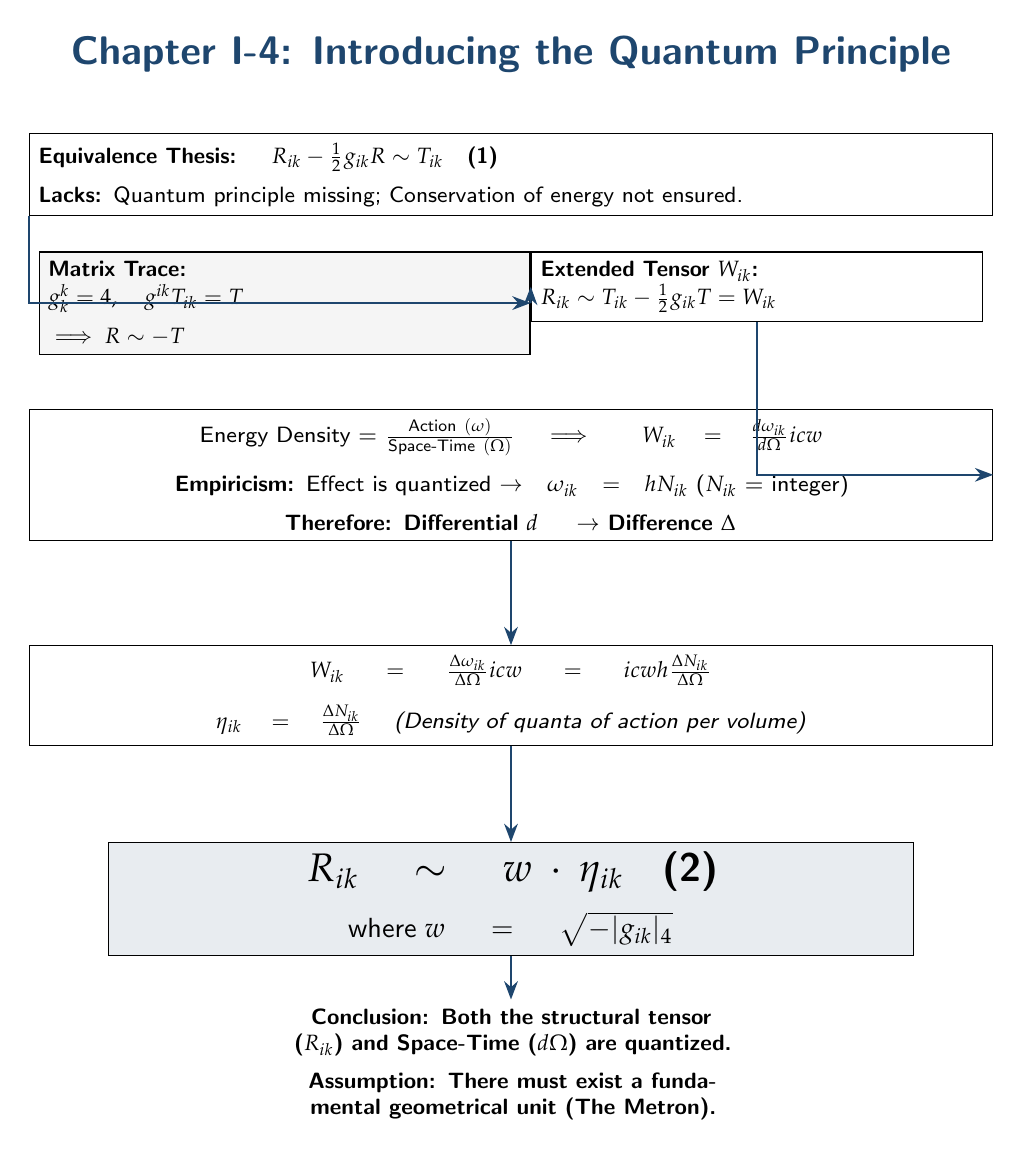
\begin{tikzpicture}[
    node distance=0.5cm,
    base/.style={draw, thin, fill=white, align=left, font=\fontsize{8pt}{10pt}\selectfont\sffamily},
    arrow/.style={-{Stealth[scale=1.0]}, thick, theoryblue}
]

    % --- HEADER ---
    \node[font=\Large\bfseries\sffamily, align=center, theoryblue] at (0, 1) {Chapter I-4: Introducing the Quantum Principle};

    % --- TOP THESIS BOX ---
    \node[base, text width=12cm, anchor=north] (thesis) at (0, 0) {
        \textbf{Equivalence Thesis:} \quad $R_{ik} - \frac{1}{2}g_{ik}R \sim T_{ik} \quad \textbf{(1)}$\\[4pt]
        \textbf{Lacks:} Quantum principle missing; Conservation of energy not ensured.
    };

    % --- MATRIX TRACE BOX ---
    \node[base, text width=6cm, anchor=north west, fill=theorygray] (trace) at (-6, -1.5) {
        \textbf{Matrix Trace:}\\
        $g^k_k = 4, \quad g^{ik}T_{ik} = T$\\[4pt]
        $\implies R \sim -T$
    };

    \node[base, text width=5.5cm, anchor=north east] (wik) at (6, -1.5) {
        \textbf{Extended Tensor $W_{ik}$:}\\
        $R_{ik} \sim T_{ik} - \frac{1}{2}g_{ik}T = W_{ik}$
    };
    \draw[arrow] (thesis.south west) |- (trace.east);
    \draw[arrow] (trace.east) -- (wik.west);

    % --- QUANTIZATION ---
    \node[base, text width=12cm, anchor=north, align=center] (quant) at (0, -3.5) {
        Energy Density = $\frac{\text{Action } (\omega)}{\text{Space-Time } (\Omega)}$ $\implies W_{ik} = \frac{d\omega_{ik}}{d\Omega}icw$\\[6pt]
        \textbf{Empiricism:} Effect is quantized $\rightarrow \omega_{ik} = h N_{ik}$ ($N_{ik}$ = integer)\\[4pt]
        \textbf{Therefore: Differential $d \to$ Difference $\Delta$}
    };
    \draw[arrow] (wik.south) |- (quant.east);

    % --- DENSITY OF ACTION ---
    \node[base, text width=12cm, anchor=north, align=center] (eta) at (0, -6.5) {
        $W_{ik} = \frac{\Delta\omega_{ik}}{\Delta\Omega}icw = icwh \frac{\Delta N_{ik}}{\Delta\Omega}$\\[6pt]
        $\eta_{ik} = \frac{\Delta N_{ik}}{\Delta\Omega} \quad$ \textit{(Density of quanta of action per volume)}
    };
    \draw[arrow] (quant.south) -- (eta.north);

    % --- FINAL EQUATION ---
    \node[base, text width=10cm, anchor=north, fill=theoryblue!10, align=center] (final) at (0, -9.0) {
        \Large $R_{ik} \sim w \cdot \eta_{ik} \quad \textbf{(2)}$\\[6pt]
        \normalsize where $w = \sqrt{-|g_{ik}|_4}$
    };
    \draw[arrow] (eta.south) -- (final.north);

    % --- ASSUMPTION ---
    \node[font=\footnotesize\bfseries\sffamily, align=center, anchor=north, text width=8cm] (assum) at (0, -11.0) {
        \textbf{Conclusion:} Both the structural tensor ($R_{ik}$) and Space-Time ($d\Omega$) are quantized.\\[4pt]
        \textbf{Assumption:} There must exist a fundamental geometrical unit (The Metron).
    };
    \draw[arrow] (final.south) -- (assum.north);

\end{tikzpicture}
\end{adjustbox}
\caption{The Matrix Trace and the Transition from Differential to Difference Calculus.}
\end{figure}

\begin{tcolorbox}[colback=white, colframe=theoryred, title=\textbf{The Paradigm Shift of Equation 2}]
Equation (2) states that the curvature of space-time ($R_{ik}$) is directly proportional to the discrete density of Action Quanta ($\eta_{ik}$). 
\begin{itemize}
    \item If the right side ($\eta_{ik}$) is discrete and quantized in integer steps, the left side ($R_{ik}$) \textbf{must also be discrete}. 
    \item Therefore, the gravitational metric does not curve smoothly. It curves in jagged, quantum-like structural steps.
    \item Because space-time volumes ($\Delta \Omega$) are constrained by these integer jumps, space cannot be infinitely divided. \textbf{A fundamental geometrical unit of area must exist.}
\end{itemize}
\end{tcolorbox}
\subsection{The Structural Decomposition Bridge (Macroscopic to Microscopic)}

To mathematically bridge the macroscopic continuous tensor ($W_{km}$) to the microscopic quantized state ($\phi_{km}$), Heim proposes that the extended energy-impulse density tensor is not a monolithic entity. Instead, it is composed of a sum of four distinct structural portions ($G$):

\begin{equation}
    \alpha W_{km} = \sum_{j=1}^4 G_{(j)km}
\end{equation}
where $\alpha$ is a proportionality constant.

Heim states that $R_4$ acts as the carrier of a Hilbert function space. In the microscopic realm, the non-Hermitian metric state of $R_4$ is described by a convergent state function $\phi_{km}^i \neq \phi_{mk}^{i*}$. 

By mapping the macroscopic partial structures ($G$) directly onto these microscopic state functions, Heim establishes the fundamental proportional link using the structural eigenvalue $\lambda_{(p)}$:
\begin{equation}
    G_{(p)km} \implies \lambda_{(p)}(k,m)\phi_{km}^{(p)}
\end{equation}

This bridge is what allows Heim to formulate the exact eigenvalue equation for the geometry:
\begin{equation}
    C_{(p)}\phi_{km}^{(p)} = \lambda_{(p)}(k,m)\phi_{km}^{(p)}
\end{equation}
The macroscopic gravitational tensor ($G$) is thus entirely synonymous with the microscopic geometric curvature steps ($\lambda$) acting on the discrete space-time connections ($\phi$).

% ==============================================================================
\textit{MBB Lectures, Chapter 4, pp. 30-38}

Before we move on to Chapter 4, we must address the \textbf{mesofield} (from the Greek \textit{meso}, meaning ``between''), a component of the gravitational field equivalent to the magnetic field.

\subsection{Detour: GravitoElectroMagnetism (GEM)}

Researching the term ``meso'' reveals its important role in the modification of Newton's laws. Heim developed this field from the purely mathematical time-varying gravitational field. Today, it is recognized (apart from the proportionality coefficients) as arising from the linearization of the field equations of General Relativity (ART) in the case of weak fields, known as the \textbf{gravitational magnetic field}.

Heim assumes that the mesofield and the gravitational field induce each other. Below is a comparison between Heim's formulations and standard GEM:

\paragraph{Heim's Formulation:}
\begin{align}
    \alpha \nabla \cdot \vec{g} &= -\sigma \tag{5} \\
    \beta \nabla \cdot \vec{\mu} &= -\sigma \nabla \cdot \vec{f} \tag{6} \\
    \nabla \times \vec{g} &= -\beta \dot{\vec{\mu}} + \frac{\sigma}{\alpha} \vec{f} \tag{7} \\
    \nabla \times \vec{\mu} &= \alpha \dot{\vec{g}} - \sigma \vec{\nu} \tag{8}
\end{align}

\paragraph{Standard GEM Formulation:}
\begin{align}
    \nabla \cdot \vec{g} &= -4 \pi G \sigma \tag{5*} \\
    \nabla \cdot \vec{B}_g &= 0 \tag{6*} \\
    \nabla \times \vec{g} &= -\dot{\vec{B}}_g \tag{7*} \\
    \nabla \times \vec{B}_g &= \frac{1}{\omega^2}(\dot{\vec{g}} - 4 \pi \sigma \vec{\nu}) \tag{8*}
\end{align}

\noindent \textbf{Definitions:} $\alpha, \beta$: field constants; $\vec{g}, \vec{\mu}$: Gravitational and meso-field; $\vec{B}_g$: Gravitational magnetic field; $\sigma$: Differential mass density; $\vec{\nu}$: Velocity field; $\vec{f}$: auxiliary functions; $\omega$: gravitational propagation velocity. Notably, in Heim's theory, $\sigma$ can take values $< 0$.

\subsection{Description of the Unified Field}
\textit{Basic Structure, Volume 1, Chapter 1-3: Space-Time Processes}

I combined gravitational and electromagnetic space-time effects together in Minkowski space (imaginary time $x_4 = ict$). It seemed reasonable to combine these two field tensors into a \textbf{unified field tensor}.

Unfortunately, an ambiguity arises when forming a vector divergence in Minkowski space from these field tensors. This divergence results in four-vectors composed of matter and charge fluxes. However, this ambiguity reduces to two possibilities if we require that Maxwell's equations and the law of gravity arise as special cases when the opposing field vanishes.

If one asserts a connection to existing experience, as one must, one path fits our experience perfectly. From the field tensor $f_{ik}$, we formulate the unified energy density tensor:
\begin{equation}
    T^i_k = f_{kn}f^{in} \tag{15}
\end{equation}
Because energy-matter equivalence assigns an inertial mass to each energy, this \textbf{non-Hermitian} energy-density tensor naturally generalizes here.

\subsubsection{Hermitian and Symmetric Tensors}
As usual in mathematics:
\begin{itemize}
    \item \textbf{Symmetric:} A tensor whose components are real and whose indices commute ($T_{ik} = T_{ki}$).
    \item \textbf{Hermitian:} If it contains complex components, complex conjugation must be performed alongside index transposition ($T_{ik} = T^*_{ki}$).
\end{itemize}
The general energy density tensor appears to be a \textbf{non-Hermitian matrix} due to the interaction between gravity and the source of the field.

\subsubsection{The Electromagnetic Case}
For the electromagnetic case alone, the tensor is written:
\begin{equation}
    T^{(E)}_{ik} = W_{ik} + \Phi_{ik}, \qquad W_{ik} = W_{ki} \approx V_{ik} \tag{1}
\end{equation}
Where $W_{ik}$ is the Hermitian part and $\Phi_{ik}$ is the non-Hermitian part:
\begin{equation}
    \Phi_{ik} = -\Phi_{ki}; \quad \Phi_{12} = \varphi_3; \quad \Phi_{13} = -\varphi_2; \quad \Phi_{23} = \varphi_1; \quad \Phi_{j,4} = -\varphi_j \tag{2}
\end{equation}
The vector product $\vec{\varphi}$ is defined as:
\begin{equation}
    \vec{\varphi} \sim \vec{g} \times \left( \vec{E} + \vec{H} \sqrt{\frac{\mu_0}{\epsilon_0}} \right)
\end{equation}
Where $\sqrt{\mu_0/\epsilon_0}$ is the characteristic impedance of empty space. If the gravitational vector $\vec{g}$ is zero, we return to the pure Hermitian tensor $V_{ik}$:
\begin{equation}
    V^k_i = f^{kl}f_{il} - \frac{1}{4} \delta^k_i f_{mn}f^{mn} \tag{4}
\end{equation}

\subsubsection{Comparison with General Relativity}
In General Relativity, the metric fundamental tensor $g_{ik} = g_{ki}$ leads to Christoffel symbols:
\begin{equation}
    \christoffel{i}{kl} = \christoffel{i}{lk} = \frac{1}{2}g^{im} \left( \frac{\partial g_{km}}{\partial x^l} + \frac{\partial g_{ml}}{\partial x^k} - \frac{\partial g_{kl}}{\partial x^m} \right) \tag{5}
\end{equation}
Einstein's conservation principle requires that the divergence vanish: $T^{ik}_{;k} = 0$. This leads to the Einstein field equations:
\begin{equation}
    R_{ik} - \frac{1}{2}g_{ik}R \sim V_{ik} \tag{8}
\end{equation}

However, Heim asserts that the unified energy density tensor is non-Hermitian ($T_{ik} \neq T_{ki}$). While anti-Hermitian components cancel in the additive process of the metric $ds^2$ (returning to a Riemannian metric), they persist in the Christoffel symbols and the curvature tensor:
\begin{equation}
    \widehat{\christoffel{i}{kl}} \neq \widehat{\christoffel{i}{lk}}, \quad R_{ik} \neq R_{ki} \tag{11-12}
\end{equation}
Heim designs a new non-Hermitian tensor equation:
\begin{equation}
    \hat{R}_{ik} - \frac{1}{2}\hat{g}_{ik}\hat{R} \sim \hat{T}_{ik} \tag{14}
\end{equation}

\textbf{The Conservation Flaw:} The non-Hermitian tensor $T_{ik}$ does not satisfy the conservation of energy and momentum ($T^{ik}_{;k} \neq 0$). Heim states:
\begin{fancyquote}
    We can calmly accept this flaw. Due to the statistical nature of the process, these statements within the microcosm do not need to be applied exactly. We just need to see if these elements that violate conservation laws can be cancelled out later.
\end{fancyquote}

\hr

\begin{reflectionbox}[title={Reflections: The Divergence Issue}]
The final step in General Relativity is that the energy tensor must have zero divergence due to conservation laws. Geometrically, the Einstein tensor on the left must also have zero divergence. This is likely why Einstein insisted on Hermitian unified field theory even when criticized by Pauli.

However, Heim asserts that his unified field is non-Hermitian and the divergence \textbf{cannot} be zero. In standard physics, this route is a dead end—the theory would fail immediately. What should we do?
\end{reflectionbox}

\textbf{Questions for this Section:}
\begin{itemize}
    \item[\fbox{?}] \textbf{Q.03:} If it's Hermitian, the divergence is zero. Please elaborate on why Heim accepts non-zero divergence.
    \item[\fbox{?}] \textbf{Q.04:} Specific expressions for the unified field tensor and the details of the construction ambiguity.
\end{itemize}

\begin{sectionrefs}
    \item \href{https://www.engon.de/protosimplex/index_e.htm}{Protosimplex (English Downloads)}.
    \item \href{https://en.wikipedia.org/wiki/Gravitoelectromagnetism}{Gravitoelectromagnetism (GEM)}: Context for the mesofield $\mu$ (gravitational magnetic field).
    \item \href{https://en.wikipedia.org/wiki/Christoffel_symbols}{Christoffel Symbols}: Notation $\genfrac{\{}{\}}{0pt}{}{i}{kl} \equiv \Gamma^{i}_{kl}$ used in the context of General Relativity.
\end{sectionrefs}

\hr

\subsection*{In-Depth: The Non-Hermitian Unified Tensor (Map I-3)}
\addcontentsline{toc}{subsection}{In-Depth: The Non-Hermitian Unified Tensor}

To realize Einstein's dream of turning the "wood" of the matter tensor into the "marble" of geometry, Heim moves from Riemannian geometry to a non-Hermitian **Cartan Geometry**. The derivation, as detailed in the Map I-3 supplements, relies on the iteration of the uniform field tensor and the analysis of complex metric components.

\subsubsection*{1. Iteration of the Field Tensor}
Heim combines the gravitational and electromagnetic field variables into a uniform field tensor $\mathbf{M}_{km}$. Through tensorial multiplication with itself and taking the trace of the spectral matrix, he derives the \textbf{Uniform Energy Impulse Density Tensor} ($T_{ik}$):
\begin{equation}
    T_{ik} = \sum_{m=1}^4 M_{im} M_{mk} = T_{ik}^+ + T_{ik}^-
\tag{I-3.1}
\end{equation}
This iteration results in a tensor that is split into a **Hermitian portion** ($T_{ik}^+$) and an **anti-Hermitian portion** ($T_{ik}^-$).

\subsubsection*{2. The Triple Metric Investigation}
Heim investigates the metric fundamental tensor $g_{ik}$ by considering the $n \ge 4$ interactions of a material field quantum ($Mq$). Each interaction produces a geodetic coordinate system $\vec{\xi}_p^{(j)}$. The metric line element is analyzed as being composed of three distinct logical parts:
\begin{equation}
    ds^2 = (g_{ik}^{(1)} + g_{ik}^{(2)} + g_{ik}^{(3)}) dx^i dx^k
\tag{I-3.2}
\end{equation}
Where:
\begin{itemize}
    \item $g_{ik}^{(1)}$ and $g_{ik}^{(3)}$ are **Symmetric/Hermitian** ($g_{ik} = g_{ki}^*$).
    \item $g_{ik}^{(2)}$ is **Asymmetric/Non-Hermitian** ($g_{ik} \neq g_{ki}^*$).
\end{itemize}
While the asymmetric portions cancel out in the scalar line element $ds^2$ (returning to a Riemannian result), they persist in the Christoffel symbols $\Gamma_{km}^i$, the Ricci tensor $R_{ik}$, and the scalar curvature $R$.

\subsubsection*{3. The Generalised Equivalence Thesis}
Heim establishes the connection between the geometric "marble" and the physical "wood" through his equivalence approach:
\begin{tcolorbox}[colback=white, colframe=theoryblue, title=\textbf{Heim's Unified Field Equation}]
The structural tensor of Cartan geometry is proportional to the uniform energy impulse density tensor:
\begin{equation}
    R_{ik} - \frac{1}{2} g_{ik} R \sim T_{ik}
\end{equation}
\end{tcolorbox}

\subsubsection*{4. Comparison with General Relativity}
Heim identifies the standard relation of General Relativity as a special case within his theory. If gravitation is isolated from other field sources ($\vec{p} \hat{=} (\vec{G}, \vec{\mu}) = 0$):
\begin{itemize}
    \item The metric becomes purely Riemannian ($g_{ik}^{(2)} = 0, g_{ik}^{(3)} = 0$).
    \item The structural tensor reduces to $R_{ik}^{(1)} - \frac{1}{2}g_{ik}^{(1)} R^{(1)}$.
    \item The matter tensor $T_{ik}$ reduces to the Maxwell canonical energy density tensor $V_{ik}$.
\end{itemize}
Thus, Heim's equation is a radical generalization where the existence of non-zero divergence in the microcosmic domain is accepted as a statistical requirement of the quantum principle, which is fully addressed in the next stage of the theory. 
% ==============================================================================
% ==============================================================================
% CHAPTER 4: THE DERIVATION OF 6 DIMENSIONS AND THE METRON
% ==============================================================================

\subsection{Finding the Empty Spectra and the Necessity of \texorpdfstring{$R_6$}{R6}}

Because space-time is defined by 4 coordinates ($k, m, p \in \{1,2,3,4\}$), the eigenvalue equation generates a massive system of tensors:
\begin{equation}
    \left. \begin{matrix} k=1\dots 4 \\ m=1\dots 4 \\ p=1\dots 4 \end{matrix} \right\} \quad 4 \times 4 \times 4 = 64 \text{ nonlinear eigenvalue equations}
\end{equation}
This means there are $4 \times 16 = 64$ possible point spectra ($\lambda_p$) describing the discrete curvature steps of $R_4$.

However, not all of these mathematical possibilities correspond to physical reality. To reduce this system, Heim investigates the symmetries of the tensor by building the matrix trace where the indices match ($i=k$).

In the macroscopic realm, building the trace of the Riemann curvature tensor ($i=k$) expands the affine connections ($\Gamma$) into:
\begin{equation}
    R_{kmp}^k = \Gamma_{kp,m}^k - \Gamma_{km,p}^k + \Gamma_{ms}^k \Gamma_{kp}^s - \Gamma_{ps}^k \Gamma_{km}^s = A_{mp}
\end{equation}
Where mathematically $A_{mp} = -A_{pm}$. Therefore, summing identical indices yields $R_{kmm}^k = 0 \implies A_{mm} = 0$.

Translating this symmetry to the microscopic eigenvalue equations, Heim finds:
\begin{equation}
    C_m \phi_{km}^k = \lambda_m(k, m) \phi_{km}^k = 0
\end{equation}
Because the state function $\phi$ is generally non-zero ($\phi \neq 0$ except in perfectly flat space), the eigenvalue itself must be zero: $\lambda_m(k, m) = 0$. 

This mathematical symmetry forces exactly \textbf{16 spectra to be empty}. Further trace analysis of the swapped indices ($\lambda_m(m, k) = 0$) reveals another 16 empty spectra. Removing the overlap between these two sets ($m=k$, which accounts for 4 spectra lying on the matrix diagonals), Heim concludes:
\begin{equation}
    16 + 16 - 4 = \textbf{28 empty spectra}
\end{equation}

Subtracting these from the original 64 equations leaves $64 - 28 = \textbf{36 non-empty eigenvalue equations}$. 

To visualize this, Heim maps the $4 \times 16 = 64$ equations into four sub-matrices (for $p=1, 2, 3, 4$). The trace rules systematically place zeros along the edges and the diagonals, effectively eliminating them from physical manifestation:

\begin{figure}[htbp]
\centering
\begin{adjustbox}{max width=0.7\textwidth}
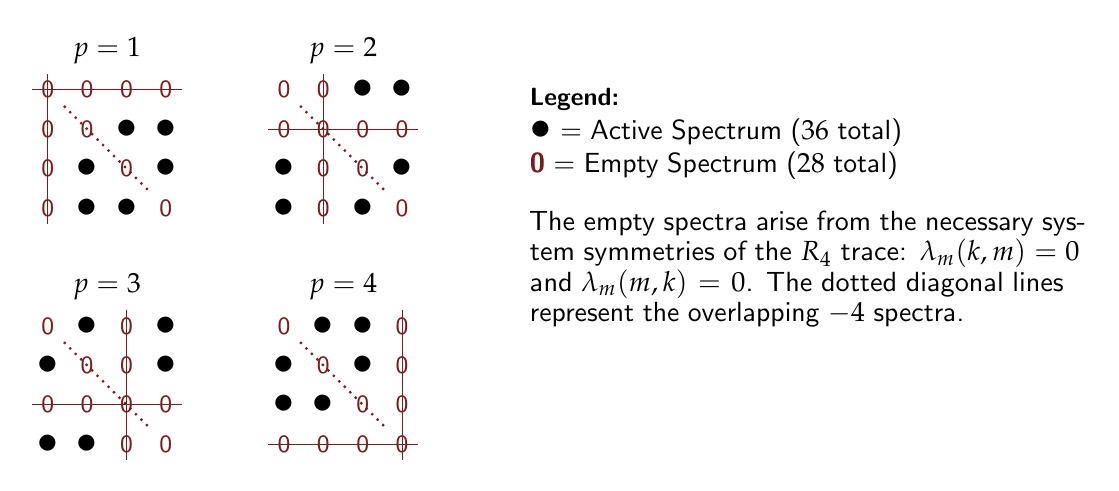
\begin{tikzpicture}
    % Define macro to draw the 4x4 grid with diagonal strike-throughs
    \def\drawgrid#1#2#3{
        \begin{scope}[shift={(#1, #2)}]
            \node[font=\bfseries\sffamily] at (0.75, 0.5) {$p=#3$};
            \foreach \x in {0,1,2,3} {
                \foreach \y in {0,1,2,3} {
                    % Rule: 0 if x == y (diagonal) OR if x == p-1 OR if y == p-1
                    \pgfmathtruncatemacro{\isp}{(( \y == (#3-1) ) || ( \x == (#3-1) ) || ( \x == \y )) ? 1 : 0}
                    \ifnum\isp=1
                        \node (n#3-\x-\y) [font=\sffamily\small, theoryred] at (\x*0.5, -\y*0.5) {0};
                    \else
                        \node (n#3-\x-\y) [font=\Large] at (\x*0.5, -\y*0.5) {$\bullet$};
                    \fi
                }
            }
            % Draw strike lines
            \pgfmathtruncatemacro{\pm}{#3-1}
            \draw[thin, theoryred] (-0.2, -\pm*0.5) -- (1.7, -\pm*0.5);
            \draw[thin, theoryred] (\pm*0.5, 0.2) -- (\pm*0.5, -1.7);
            % Draw dotted diagonal connecting the 4 overlapping empty spectra
            \draw[dotted, thick, theoryred] (n#3-0-0) -- (n#3-3-3);
        \end{scope}
    }

    % Draw the four matrices
    \drawgrid{0}{0}{1}
    \drawgrid{3}{0}{2}
    \drawgrid{0}{-3}{3}
    \drawgrid{3}{-3}{4}

    % Explanatory Text
    \node[anchor=west, font=\sffamily\small, text width=7cm] at (6, -1.5) {
        \textbf{Legend:}\\
        \Large $\bullet$ \normalsize = Active Spectrum ($36$ total)\\
        \textcolor{theoryred}{\textbf{0}} = Empty Spectrum ($28$ total)\\[10pt]
        The empty spectra arise from the necessary system symmetries of the $R_4$ trace: $\lambda_m(k,m) = 0$ and $\lambda_m(m,k) = 0$. The dotted diagonal lines represent the overlapping $-4$ spectra. 
    };
\end{tikzpicture}
\end{adjustbox}
\caption{The $4 \times 16$ Eigenvalue Spectra matrices. The 28 mathematically empty states force the remaining 36 active states to be arranged in a 6-dimensional geometry.}
\end{figure}

\subsubsection{The Improper Quotient: The Proof of Superspace}
If the material world operates with 36 active energy densities, these cannot be arranged symmetrically in a 4D tensor ($4 \times 4 = 16$) or a 5D tensor ($5 \times 5 = 25$). To conserve energy and remain invariant against coordinate transformations, these 36 non-empty spectra fit perfectly into a \textbf{$6 \times 6$ tensor} (36 components). 

Heim and Dröscher provided a formal mathematical proof for this transition known as the \textbf{Improper Quotient} (\textit{Uneigentlicher Quotient}). When analyzing the symmetry of the $R_4$ metric transition, another relationship emerges:
\begin{equation}
    \lambda_{(m)}(m, p)\phi_{mp}^i = -\lambda_{(p)}(m, m)\phi_{mm}^i
\end{equation}
For components where both eigenvalues reside in an empty spectrum ($\lambda = 0$), the equation requires a division of zero by zero:
\begin{equation}
    \phi_{mp}^i = -\frac{\lambda_{(p)}(m, m)}{\lambda_{(m)}(m, p)} \phi_{mm}^i \xrightarrow{\text{4D limit}} \frac{0}{0} \phi_{mm}^i
\end{equation}
In a continuous 4-dimensional manifold, this result is undefined. However, Heim proved (Volume 1, Page 54) that by performing the limit within a \textbf{6-dimensional superspace}, this "improper" quotient resolves into a finite, non-zero constant ($a_{mp} \neq 0$). This constant is the structural coupling that allows matter to possess mass. It proved that the higher dimensions are a mathematical necessity to resolve the singularities of 4D spacetime.

Heim mapped these 12 additional empty components into the $R_6$ energy-impulse tensor ($\mathbf{\bar{T}}$) such that the empirical space-time ($R_4$) is perfectly conserved. The dimensions $x_5, x_6$ do not affect the observable $R_3$ spatial dimensions directly, resulting in zero-values in the cross-components:

\begin{figure}[htbp]
\centering
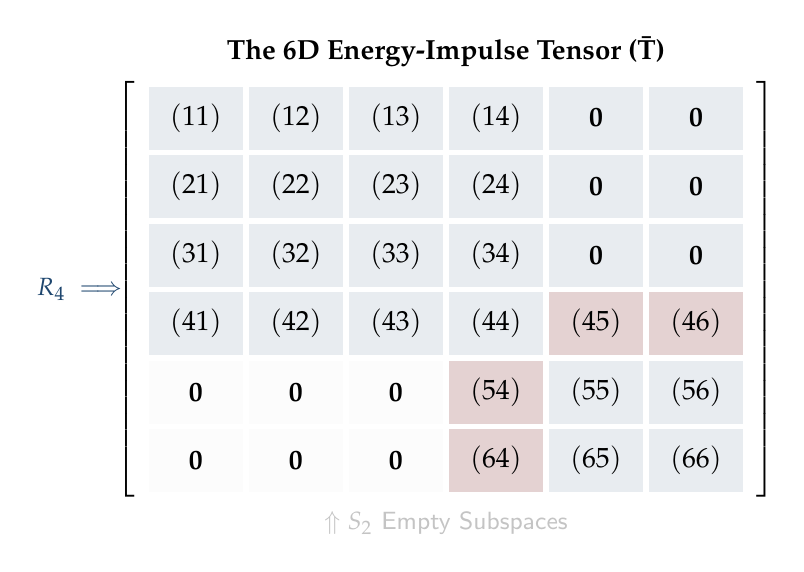
\begin{tikzpicture}
    \matrix [
        matrix of math nodes,
        left delimiter={[}, right delimiter={]},
        nodes={minimum width=1.2cm, minimum height=0.8cm, anchor=center, font=\sffamily},
        row sep=2pt, column sep=2pt,
        % Color the R4 block
        row 1/.style={nodes={fill=theoryblue!10}},
        row 2/.style={nodes={fill=theoryblue!10}},
        row 3/.style={nodes={fill=theoryblue!10}},
        row 4/.style={nodes={fill=theoryblue!10}},
        % Color the S2 cross block
        column 5/.style={nodes={fill=theorygray!30}},
        column 6/.style={nodes={fill=theorygray!30}},
        row 5/.style={nodes={fill=theorygray!30}},
        row 6/.style={nodes={fill=theorygray!30}}
    ] (tensor) {
        (11) & (12) & (13) & (14) & \mathbf{0} & \mathbf{0} \\
        (21) & (22) & (23) & (24) & \mathbf{0} & \mathbf{0} \\
        (31) & (32) & (33) & (34) & \mathbf{0} & \mathbf{0} \\
        (41) & (42) & (43) & (44) & |[fill=theoryred!20]|(45) & |[fill=theoryred!20]|(46) \\
        \mathbf{0} & \mathbf{0} & \mathbf{0} & |[fill=theoryred!20]|(54) & |[fill=theoryblue!10]|(55) & |[fill=theoryblue!10]|(56) \\
        \mathbf{0} & \mathbf{0} & \mathbf{0} & |[fill=theoryred!20]|(64) & |[fill=theoryblue!10]|(65) & |[fill=theoryblue!10]|(66) \\
    };
    
    % Labels
    \node[anchor=south] at (tensor.north) {\textbf{The 6D Energy-Impulse Tensor ($\mathbf{\bar{T}}$)}};
    \node[anchor=east, font=\sffamily\small, theoryblue] at (tensor.west) {$R_4 \implies$};
    \node[anchor=north, font=\sffamily\small, theorygray!80!black] at (tensor.south) {$\Uparrow S_2$ Empty Subspaces};
\end{tikzpicture}
\caption{The arrangement of the 36 active spectra. The structural dimensions ($x_5, x_6$) interact exclusively with Time ($x_4$) and themselves, cleanly resulting in $\mathbf{0}$ cross-components for the observable $R_3$ spatial dimensions ($x_1, x_2, x_3$).}
\end{figure}

\subsubsection{The Structure of the \texorpdfstring{$R_6$}{R6} Metric Tensor}
This arrangement is perfectly mirrored in the $6 \times 6$ fundamental metric tensor $g_{ik}^{(6)}$:
\begin{equation}
    g_{ik}^{(6)} = \left(
    \begin{array}{ccc|c|cc}
    g_{11} & g_{12} & g_{13} & g_{14} & \cellcolor{theoryred!10}0 & \cellcolor{theoryred!10}0 \\
    g_{21} & g_{22} & g_{23} & g_{24} & \cellcolor{theoryred!10}0 & \cellcolor{theoryred!10}0 \\
    g_{31} & g_{32} & g_{33} & g_{34} & \cellcolor{theoryred!10}0 & \cellcolor{theoryred!10}0 \\ \hline
    g_{41} & g_{42} & g_{43} & g_{44} & \cellcolor{theoryblue!10}g_{45} & \cellcolor{theoryblue!10}g_{46} \\ \hline
    \cellcolor{theoryred!10}0 & \cellcolor{theoryred!10}0 & \cellcolor{theoryred!10}0 & \cellcolor{theoryblue!10}g_{54} & g_{55} & g_{56} \\
    \cellcolor{theoryred!10}0 & \cellcolor{theoryred!10}0 & \cellcolor{theoryred!10}0 & \cellcolor{theoryblue!10}g_{64} & g_{65} & g_{66} \\
    \end{array}
    \right)
\end{equation}
Because the cross-terms bounded in red are strictly zero ($g_{s\sigma} = 0$ for $s \in \{1,2,3\}$ and $\sigma \in \{5,6\}$), the organizational dimensions $x_5$ and $x_6$ cannot be perceived directly by human senses or 3D instruments. They only interact with physical space indirectly through the temporal cross-terms ($g_{45}, g_{46}$, bounded in blue).

\subsubsection{The Stability Proof for 3 Real Dimensions}
To determine the algebraic nature (real vs. imaginary) of these new dimensions, Heim evaluated the metric signatures of $R_6$. He analyzed the behavior of central-force orbits (both planetary and electronic) in a hypothetical space where the number of real dimensions $p$ varies.

\begin{table}[htbp]
\centering
\renewcommand{\arraystretch}{1.5}
\begin{tabular}{clcl}
\toprule
\textbf{Variant} & \textbf{Metric Signature} & \textbf{Real Dims ($p$)} & \textbf{Physical Viability} \\
\midrule
\rowcolor{theoryblue!5}
\textbf{a} & $(+ + + - + +)$ & $p=5$ & \textbf{Rejected:} $p>4$ causes orbits to degrade into logarithmic spirals.\\
\textbf{b} & $(+ + + - + -)$ & $p=4$ & \textbf{Rejected:} Violates approximate invariance of the Poincaré group.\\
\textbf{c} & $(+ + + - - +)$ & $p=4$ & \textbf{Rejected:} Violates approximate invariance of the Poincaré group.\\
\rowcolor{theorygray!50}
\textbf{d} & $(+ + + - - -)$ & $p=3$ & \textbf{Accepted:} Only $p \le 3$ permits stable macroscopic orbits. \\
\bottomrule
\end{tabular}
\caption{Determination of the algebraic character of dimensions $x_5, x_6$ in $R_6$.}
\end{table}

Heim demonstrated mathematically that for $p > 3$, closed, stable orbits are geometrically impossible. In a 4D or 5D real space, the gravitational and electromagnetic inverse-square laws become inverse-cube or higher. This causes any orbiting body to instantly shift into a logarithmic spiral. In a 4D spatial world, electrons would spiral into the nucleus in a fraction of a second, and planets would collapse into their stars.

Because $p=4$ causes circular paths to degrade, the physical universe is strictly limited to $p=3$ real dimensions. The $R_6$ signature $(+ + + - - -)$ is the only one that permits stable matter, proving that $x_5$ and $x_6$ must be imaginary organizational dimensions ($\iu\varepsilon, \iu\eta$).


\section{The Derivation of the Metron (\texorpdfstring{$\tau$}{tau})}

\textit{References: MBB Lecture Transcript; Application of the Corrected Gravitation Law Maps; Elementarstrukturen der Materie (Anhang II)}

Having established that space-time is discrete and 6-dimensional, Heim needed to find the absolute size of the "pixel" of the universe. This is the derivation of the \textbf{Metron} ($\tau$).

Heim returned to the \textbf{Corrected Gravitation Law} derived in Section \ref{sec:grav_dynamics}. Because the gravitational field possesses field mass, the square of the stable orbital speed ($\varphi$) at a distance $r$ is non-linear:
\begin{equation}
    r q e^q = A \left(1 - \frac{\gamma m^3 r}{\hbar^2}\right)^2
\end{equation}
This equation features an Inner Limit ($r_0$), a distance where gravitational attraction acts as an absolute barrier (conceptually similar to the Schwarzschild radius).

Heim performed a limit analysis on a hypothetical Elementary Mass ($m \to 0$). As the mass of a particle shrinks to zero, two conflicting infinities arise:
\begin{enumerate}
    \item The inner gravitational limit shrinks to zero ($r_0 \to 0$).
    \item The quantum Compton wavelength expands to infinity ($\lambda \to \infty$).
\end{enumerate}

Standard calculus treats $0 \times \infty$ as undefined. To resolve this, Heim performed a series expansion on the product of these two limits. He discovered that the product does not equal zero, but converges to a finite universal constant.

\begin{tcolorbox}[colback=white, colframe=theoryred, title=\textbf{The Fundamental Geometrical Constant (The Metron)}]
\begin{equation}
    \lim_{m \to 0} (r_0^* \cdot \lambda) = \pi \gamma \hbar = \tau
\end{equation}
where $\gamma$ is the gravitational constant and $\hbar$ is the reduced Planck constant. This constant $\tau$ is the \textbf{Metron}. It has the units of Area ($\text{m}^2$), not length. 
\begin{equation*}
    \tau \approx 6.15 \times 10^{-70} \text{ m}^2
\end{equation*}
\end{tcolorbox}

\subsubsection{Comparison to the Planck Area}
In mainstream quantum physics, dimensional analysis of the fundamental constants ($G, c, \hbar$) yields the Planck Area ($l_p^2 \approx 2.6 \times 10^{-70} \text{ m}^2$). Modern Loop Quantum Gravity postulates that space is quantized on this scale. 

Astonishingly, Heim arrived at the exact same physical scale decades earlier. However, while the Planck Area is derived purely from dimensional analysis (a mathematical coincidence of units), Heim's Metron ($\tau$) is derived dynamically from the limit of the gravitational field mass. Heim's derivation provides the actual geometric mechanism for \textit{why} space quantizes at this scale.

\subsubsection{The Error of the Infinitesimal Calculus}
In the final appendix of Volume 1, Heim identifies the "Historical Error" that has prevented the unification of physics. He argues that the use of Infinitesimal Calculus ($\diff x \to 0$) is physically invalid because it assumes that two points can be closer than the Metron distance ($\sqrt{\tau}$).

When a standard physicist calculates the gravitational force at $r \to 0$, the equation yields an \textit{infinite} force (a singularity). In Heim's discrete geometry, the denominator can never be smaller than $\tau$. By replacing the differential quotient with the \textbf{Metron Selector} ($\ethop$), the "singularities" of General Relativity and the "infinities" of Quantum Field Theory simply vanish.


\section{Particles as Cyclic Periodic Processes}
\label{sec:particle_dynamics}

\textit{References: MBB Lecture Transcript; Map "Particles as cyclic periodic processes" (Page 4)}

In Heim Theory, a particle is not an object inserted \textit{into} space; it is a localized, dynamic structural deformation \textit{of} the space itself. Heim defines ponderable particles as \textbf{Cyclic Periodic Processes of Interchanges} in $R_6$, also known as \textbf{Condensor Fluxes}.

\subsection{The Flux Algebra and Stability Criterion}
A Condensor Flux is a dynamic process where metric information (structural condensation) flows through the dimensions $x_1 \dots x_6$. For a particle to exist as a stable, observable entity in our 3D space, this flow must satisfy a strict geometrical boundary condition in the time coordinate ($x_4$).

Heim developed a \textbf{Flux Algebra} to evaluate these flows:
\begin{itemize}
    \item \textbf{Stable Particles (e.g., Electron, Proton):} The flux of partial structures completes a full cycle and closes upon itself exactly within a specific period duration. The initial metric conditions are perfectly restored.
    \item \textbf{Unstable Particles (Radioactive Decay):} The flux fails to close upon itself. The structural metric "leaks" or fails to complete the cycle within the required period duration, causing the geometric knot to unravel (decay into lighter, stable configurations).
\end{itemize}

\begin{figure}[htbp]
\centering
\begin{adjustbox}{max width=0.85\textwidth}
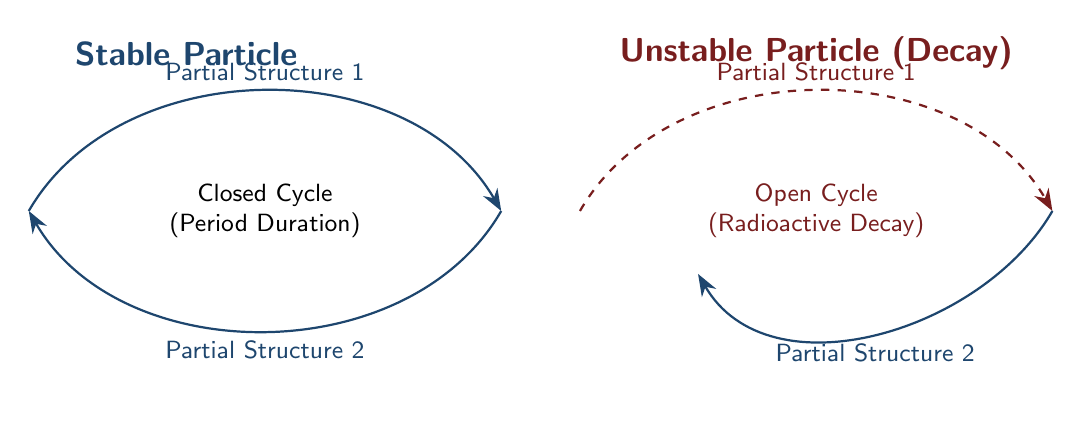
\begin{tikzpicture}[
    node distance=0.4cm,
    base/.style={draw, thin, fill=white, align=left, font=\fontsize{9pt}{11pt}\selectfont\sffamily},
    arrow/.style={-{Stealth[scale=1.2]}, thick, theoryblue},
    dashedarrow/.style={-{Stealth[scale=1.2]}, dashed, thick, theoryred}
]

    % --- Stable Cycle ---
    \node[font=\large\bfseries\sffamily, theoryblue] at (-3, 2) {Stable Particle};
    
    \draw[arrow] (-5, 0) to[out=60, in=120] node[above, font=\small\sffamily] {Partial Structure 1} (1, 0);
    \draw[arrow] (1, 0) to[out=-120, in=-60] node[below, font=\small\sffamily] {Partial Structure 2} (-5, 0);
    
    \node[font=\small\sffamily, align=center] at (-2, 0) {Closed Cycle\\(Period Duration)};

    % --- Unstable Cycle ---
    \node[font=\large\bfseries\sffamily, theoryred] at (5, 2) {Unstable Particle (Decay)};
    
    \draw[dashedarrow] (2, 0) to[out=60, in=120] node[above, font=\small\sffamily] {Partial Structure 1} (8, 0);
    \draw[arrow] (8, 0) to[out=-120, in=-60] node[below, font=\small\sffamily] {Partial Structure 2} (3.5, -0.8); % Fails to close
    
    \node[font=\small\sffamily, align=center, theoryred] at (5, 0) {Open Cycle\\(Radioactive Decay)};

\end{tikzpicture}
\end{adjustbox}
\caption{The Geometric Stability Criterion: Particles are cyclic metric exchange processes in $R_6$.}
\end{figure}

\subsubsection{The Chronon Oscillation: Real and Virtual States}
A fundamental revelation of Heim's discrete geometry (Volume 1, Page 189) is that elementary particles are not persistent objects, but \textbf{High-Frequency Oscillations}. 

Because time is quantized into Chronons ($\vartheta$), the World Selector eigenvalue equations must be solved anew at every time-step. Heim demonstrates that a stable particle actually oscillates between two states every Chronon:
\begin{enumerate}
    \item \textbf{The Real State:} The metron flux projects into $R_3$, possessing measurable mass and coordinates.
    \item \textbf{The Virtual State:} The flux rotates entirely into the imaginary organizational dimensions ($S_2$), appearing as a "vacuum fluctuation."
\end{enumerate}
This "Metron Heartbeat" occurs so rapidly ($1/\vartheta \approx 10^{42} \text{ Hz}$) that macroscopic instruments perceive a solid, persistent particle. However, this oscillation is the true source of \textbf{Zero-Point Energy}.

\subsection{Spin in \texorpdfstring{$R_6$}{R6}: Fermions and Bosons}
Because these fluxes are cyclic, they inherently possess angular momentum, or \textbf{Spin}. In $R_6$, total spin is a complex interplay between the real spatial dimensions ($R_3$) and the imaginary auxiliary dimensions ($T \cup S_2$). 

Heim defines the total spin in $R_6$ as:
\begin{equation}
    \text{Total Spin} = \sigma \hbar, \quad \text{where } \sigma = \iu(s + J(-1)^P)
\end{equation}
Where:
\begin{itemize}
    \item $s = P/2$: The Isomorphism Spin (spin in the imaginary coordinates $x_4 \dots x_6$). $P$ is an integer.
    \item $J = Q/2$: The Spin in Space ($R_3$). $Q$ is an integer.
\end{itemize}

This single geometric formula naturally derives the fundamental difference between the two classes of particles in the universe, providing the geometric origin of the \textbf{Pauli Exclusion Principle}.

\begin{figure}[htbp]
\centering
\begin{adjustbox}{max width=0.85\textwidth}
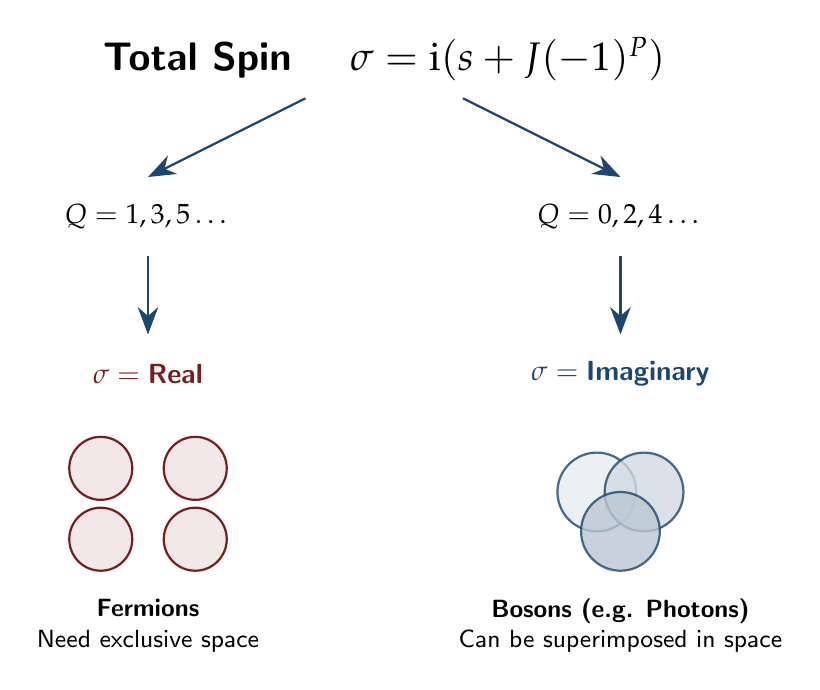
\begin{tikzpicture}[
    node distance=0.4cm,
    arrow/.style={-{Stealth[scale=1.5]}, thick, theoryblue}
]

    % Top Equation
    \node[font=\Large\bfseries\sffamily] (top) at (0,0) {Total Spin \quad $\sigma = \iu(s + J(-1)^P)$};
    
    % Split arrows
    \draw[arrow] (-1, -0.5) -- (-3, -1.5);
    \draw[arrow] (1, -0.5) -- (3, -1.5);

    % Left Branch (Fermions)
    \node[font=\bfseries\sffamily] (odd) at (-3, -2) {$Q = 1, 3, 5 \dots$};
    \draw[arrow] (-3, -2.5) -- (-3, -3.5);
    \node[font=\bfseries\sffamily, theoryred] (real) at (-3, -4) {$\sigma = \text{Real}$};
    
    % Fermion Circles (Not overlapping)
    \draw[thick, theoryred, fill=theoryred!10] (-3.6, -5.2) circle (0.4);
    \draw[thick, theoryred, fill=theoryred!10] (-3.6, -6.1) circle (0.4);
    \draw[thick, theoryred, fill=theoryred!10] (-2.4, -5.2) circle (0.4);
    \draw[thick, theoryred, fill=theoryred!10] (-2.4, -6.1) circle (0.4);
    
    \node[font=\sffamily\small, align=center] at (-3, -7.2) {\textbf{Fermions}\\ Need exclusive space};

    % Right Branch (Bosons)
    \node[font=\bfseries\sffamily] (even) at (3, -2) {$Q = 0, 2, 4 \dots$};
    \draw[arrow] (3, -2.5) -- (3, -3.5);
    \node[font=\bfseries\sffamily, theoryblue] (imag) at (3, -4) {$\sigma = \text{Imaginary}$};
    
    % Boson Circles (Overlapping)
    \draw[thick, theoryblue, fill=theoryblue!10, opacity=0.8] (2.7, -5.5) circle (0.5);
    \draw[thick, theoryblue, fill=theoryblue!20, opacity=0.8] (3.3, -5.5) circle (0.5);
    \draw[thick, theoryblue, fill=theoryblue!30, opacity=0.8] (3.0, -6.0) circle (0.5);
    
    \node[font=\sffamily\small, align=center] at (3, -7.2) {\textbf{Bosons (e.g. Photons)}\\ Can be superimposed in space};

\end{tikzpicture}
\end{adjustbox}
\caption{The Spin Analysis in $R_6$. The integer $Q$ dictates whether the metric structure possesses real spin (displacing spatial volume) or imaginary spin (allowing superposition).}
\end{figure}

\subsubsection{The Isomorphism Spin ($P$) and Anti-Matter}
To account for the existence of anti-particles without relying on Dirac's "sea of negative energy," Heim introduced the \textbf{Isomorphism Spin ($P$)}. While the spatial spin ($Q$) governs the particle's angular momentum in $R_3$, the Isomorphism Spin ($P$) defines the particle's rotational orientation in the imaginary organizational coordinates ($x_5, x_6$). 

Heim proves that \textbf{Matter} corresponds to a positive isomorphic rotation ($+P$), while \textbf{Anti-Matter} corresponds to a mirrored isomorphic rotation ($-P$). This provides a purely geometric definition of \textbf{CP-Symmetry}. A positron is not an electron with "opposite charge"; it is a metron flux knot rotating in the opposite direction along the $S_2$ structural axes.

\section{The Internal Structure of Elementary Particles}
\label{sec:internal_structure}

\textit{References: MBB Lecture Transcript; Map "Inner density of protosimplexes" (Page 5)}

In 1976, Heim famously challenged Werner Heisenberg's assertion that one "shouldn't ask about the interior of elementary particles." Because Heim's particles are 6-dimensional Condensor Fluxes, they possess a highly specific internal geometric architecture when projected into our 3D space.

Heim calculates that the "density" of the metric anomalies (the Protosimplexes) decreases outward from the center of the flux cycle, creating four distinct concentric zones. 

\begin{figure}[htbp]
\centering
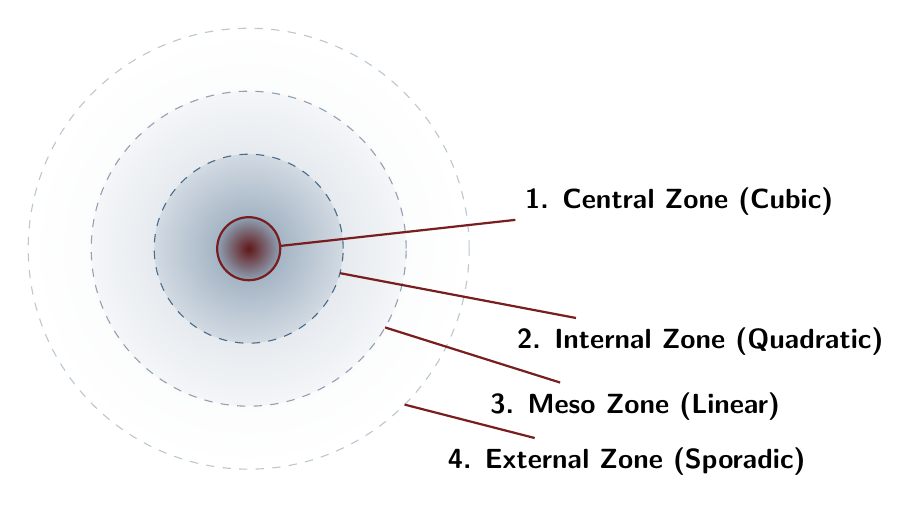
\begin{tikzpicture}[
    pin edge={-{Stealth}, thick, theoryred}
]
    % Draw concentric spheres using radial shading to represent metric density
    \shade[inner color=theoryblue!5, outer color=white] (0,0) circle (2.8);
    \shade[inner color=theoryblue!20, outer color=theoryblue!5] (0,0) circle (2.0);
    \shade[inner color=theoryblue!50, outer color=theoryblue!20] (0,0) circle (1.2);
    \shade[inner color=theoryred!80!black, outer color=theoryblue!50] (0,0) circle (0.4);
    
    % Draw boundaries
    \draw[thin, theoryblue!30, dashed] (0,0) circle (2.8);
    \draw[thin, theoryblue!50, dashed] (0,0) circle (2.0);
    \draw[thin, theoryblue!80, dashed] (0,0) circle (1.2);
    \draw[thick, theoryred] (0,0) circle (0.4);
    
    % Pointers and Labels using TikZ polar coordinates (angle:radius)
    \node[coordinate, pin={[pin distance=3cm, pin edge={theoryred, thick}]5:{\sffamily\bfseries 1. Central Zone (Cubic)}}] at (5:0.4) {};
    \node[coordinate, pin={[pin distance=2.2cm, pin edge={theoryred, thick}]345:{\sffamily\bfseries 2. Internal Zone (Quadratic)}}] at (345:1.2) {};
    \node[coordinate, pin={[pin distance=1.4cm, pin edge={theoryred, thick}]330:{\sffamily\bfseries 3. Meso Zone (Linear)}}] at (330:2.0) {};
    \node[coordinate, pin={[pin distance=0.6cm, pin edge={theoryred, thick}]315:{\sffamily\bfseries 4. External Zone (Sporadic)}}] at (315:2.8) {};
    
\end{tikzpicture}
\caption{The geometric cross-section of an elementary particle (Condensor Flux) in $R_3$. The metric density (Protosimplex concentration) decreases radically from the impenetrable core to the sporadic periphery.}
\end{figure}

\begin{table}[htbp]
\centering
\renewcommand{\arraystretch}{1.5}
\begin{tabular}{lll}
\toprule
\textbf{Zone} & \textbf{Metric Density} & \textbf{Characteristic} \\
\midrule
\rowcolor{theorygray!30}
\textbf{1. Central Zone} & Cubic & Impenetrable \\
\textbf{2. Internal Zone} & Quadratic & \\
\rowcolor{theorygray!30}
\textbf{3. Meso Zone} & Linear & Penetrable \\
\textbf{4. External Zone} & Sporadically Occupied & Penetrable \\
\bottomrule
\end{tabular}
\caption{The internal density distribution of Protosimplexes in a Heim Particle.}
\end{table}

\subsection{The Strong Force as Geometric Zone Overlap}
In the Standard Model, the nucleus of an atom is held together by the Strong Force, mediated by the exchange of gluons. Heim Theory provides a purely structural alternative that eliminates the need for virtual particle exchange.

Heim proves (Volume 1, Page 72) that the \textbf{Strong Nuclear Force} is the result of the \textbf{Meso-Zone} and \textbf{Internal Zone} of two baryons physically occupying the same metron grid coordinates. 

When the distance between two protons reaches the radius of their Meso-Zones, the structural compressor ($\varsigma^{\underline{i}}_{klm}$) identifies the two separate "knots" as a single, correlated geometric system. The "Force" is simply the $R_6$ lattice's resistance to being pulled apart once these high-density metron regions have merged. This geometrically explains why the Strong Force has such a short range and why it becomes repulsive if the particles are pushed too close (geometric saturation).

\begin{mbbcite}
    \textbf{Spacetime vs. Quarks:} Heim's model predates the widespread acceptance of Quantum Chromodynamics (QCD). In Heim's view, the scattering experiments that led physicists to invent "Quarks" and "Gluons" were actually detecting these four concentric zones of metric density. Quarks are thus interpreted not as independent sub-particles, but as the localized mathematical nodes of the $R_6$ metric flux.
\end{mbbcite} 
\section{The Mass Formula and Geometric Quantum Numbers}
\label{sec:mass_formula}

\textit{References: MBB Lecture Transcript; Map "Generation of quantum numbers" (Pages 4 \& 5); Elementarstrukturen der Materie (Kap. 4 \& Anhang I)}

To calculate the exact mass of these particles, Heim translates the geometry of the Condensor Flux into a set of \textbf{Geometric Quantum Numbers}. Unlike the quantum numbers in the Standard Model (which are often assigned empirically to balance equations), Heim's quantum numbers are strictly derived from the geometric properties of the $R_6$ flux.

\begin{table}[htbp]
\centering
\renewcommand{\arraystretch}{1.4}
\begin{tabular}{lll}
\toprule
\textbf{Number} & \textbf{Selecting Conditions} & \textbf{Empirical Correspondence} \\
\midrule
\rowcolor{theoryblue!5}
\textbf{$k$} & $1, 2$ & Configuration number (Baryon number $B = k-1$) \\
\textbf{$P$} & $0 \dots k+1$ & Isomorphism spin \\
\rowcolor{theoryblue!5}
\textbf{$Q$} & $k-1$ (for $P = 2-k$) \newline $2k-1$ (for $P = 2k-1$) & Spin in space \\
\textbf{$\kappa$} & $0, 1$ ($\kappa=1 \to \text{doublet}$) & Doublet \\
\rowcolor{theoryblue!5}
\textbf{$C$} & $f(k, P, Q, \kappa, \epsilon)$ & Configuration distributor (Strangeness) \\
\textbf{$q_x$} & $f(C, k, P, Q, \kappa, \epsilon, x)$ & Charge quantum number ($x$ numbers internal components) \\
\rowcolor{theoryblue!5}
\textbf{$N$} & $0 \dots N_{\max}$ & Resonance allocation ($0 = \text{ground state}$) \\
\textbf{$\epsilon$} & $+1, -1$ & Time helix direction (Temporal direction of rotation; Particle / Anti-particle) \\
\bottomrule
\end{tabular}
\caption{Geometrical quantum numbers derived from $R_6$ and their empirical equivalents.}
\end{table}

\subsubsection{The Geometric Origin of Baryon Number}
In the Standard Model, the Baryon Number ($B$) is conserved empirically. In Heim Theory (Volume 1, Page 307), it is a strict geometric outcome of the \textbf{Configuration Number ($k$)}. Heim defines the relationship:
\begin{equation}
    B = k - 1
\end{equation}
This derivation proves that "Baryonness" is not a separate physical charge; it is a manifestation of the structural knot's configuration ($k$). A particle is a "Baryon" ($B=1$) if its internal metron condensation flux forces a configuration index of $k=2$, and a "Meson" ($B=0$) if $k=1$.

The allocation of these numbers is strictly governed by polynomial auxiliary conditions. For the spin in space ($Q$) to increase ($Q \to Q+k$), the isomorphism spin must satisfy:
\begin{equation}
    P - P(k+1) + 5k = 2(k^2+1) \quad \implies \quad P = 2-k \text{ or } P = 2k-1
\end{equation}
Similarly, the configuration distributor $C$ (which acts as the geometric equivalent of Strangeness) is constrained by the sum of charge quanta $q_i$ across all possible multiplets for a given configuration $k$:
\begin{equation}
    S_k = (-1)^x \Sigma_s \text{ (sum of } q_i \text{ of all possible multiplets for } k)
\end{equation}

\subsection{Multiplets and the 25 Ground States}

By inputting the fundamental natural constants ($\gamma, h, \varepsilon_0, \mu_0, c, \pi$) and the basic set $\{+1, 0, -1\}$ into his \textbf{Universal Mass Equation}, Heim generates the discrete point spectrum of all ponderable particles:

\begin{equation}
    m(N, k, P, Q, \kappa) = m_e \cdot \left[ 1 + \sum_{j} f_j(k, P, Q, \kappa) \cdot \eu^{-N \lambda_j} \right]
\end{equation}

A major failure of the Standard Model is that it cannot explain \textit{why} there are exactly the number of fundamental particles we observe; it merely catalogs them. By solving the World Selector equations for the $c$- and $d$-Hermetry forms, Heim proved that the $R_6$ hyperstructure only permits exactly \textbf{25 stable and metastable ground states} ($N=0$). 

The configuration number $k$ perfectly splits these 25 ground states into their observed families (Multiplets):
\begin{itemize}
    \item \textbf{$k=1$:} Yields exactly 5 Multiplets. This corresponds entirely to all \textbf{Mesons}.
    \item \textbf{$k=2$:} Yields exactly 6 Multiplets. This corresponds entirely to all \textbf{Baryons}.
\end{itemize}

\subsubsection{The Resonance Law (Higher Eigenvalues)}
Every ground state particle ($N=0$) is the "fundamental tone" of a geometric flux. However, the World Selector allows for higher-order integer solutions ($N>0$). These states correspond to the unstable, high-energy resonances observed in collider experiments (e.g., the $\Delta$ or $\Sigma^*$ resonances). Because the underlying geometry is quantized, any particle discovered in an accelerator that is not one of the 25 ground states is geometrically proven to be merely a transient, excited resonance ($N > 0$) of one of these fundamental base structures.

When the specific quantum states $(kPQ\kappa)C(q_x)$ are evaluated for the ground state ($N=0$), the formula exactly conforms with experience, outputting the masses of our familiar universe:

\begin{table}[htbp]
\centering
\renewcommand{\arraystretch}{1.3}
\begin{tabular}{@{}llcc@{}}
\toprule
\textbf{Particle} & \textbf{Geometric Quantum Numbers} & \textbf{Theor. Mass (MeV)} & \textbf{Exp. Mass (MeV)} \\
& $(k, P, Q, \kappa)\; q_x (C)$ & & \\
\midrule
\rowcolor{theoryblue!5}
Electron ($e^-$) & $(1, 1, 1, 0)\; -1\; (0)$ & 0.510999 & 0.511 \\
Muon ($\mu^-$) & $(1, 1, 1, 1)\; -1\; (0)$ & 105.6586 & 105.658 \\
\rowcolor{theoryblue!5}
Pion ($\pi^\pm$) & $(1, 2, 0, 0)\; \pm 1\; (0)$ & 139.5659 & 139.570 \\
Kaon ($K^+$) & $(1, 1, 0, 1)\; +1\; (+1)$ & 493.6634 & 493.677 \\
\rowcolor{theorygray!20}
Proton ($p$) & $(2, 1, 1, 0)\; +1\; (0)$ & 938.2719 & 938.272 \\
\rowcolor{theorygray!20}
Neutron ($n$) & $(2, 1, 1, 0)\; \;\;0\; (0)$ & 939.5653 & 939.565 \\
Lambda ($\Lambda$) & $(2, 0, 1, 0)\; \;\;0\; (-1)$ & 1115.592 & 1115.683 \\
Sigma ($\Sigma^+$) & $(2, 2, 1, 0)\; +1\; (-1)$ & 1189.384 & 1189.370 \\
Omega ($\Omega^-$) & $(2, 0, 3, 0)\; -1\; (-3)$ & 1672.361 & 1672.450 \\
\bottomrule
\end{tabular}
\caption{Selection from Heim's theoretical mass spectrum (Volume 1, Page 308). The theoretical masses are derived entirely from the geometric quantum numbers of the $R_6$ hyperstructure, without using empirical quark masses or the Higgs mechanism.}
\end{table}

\subsection{From the World Selector to the Fundamental Constants}

To understand how Heim’s theory bridges the gap between pure geometry and physical mass, one must look at the final integral of the World Selector (Equation W5, derived in the Metron Calculations). 

When Heim set out to calculate the mass of the electron ($m_e$), he did not use phenomenological inputs or a Higgs mechanism. Instead, he mapped the electron's geometric quantum numbers ($k=1, P=1, Q=1$) into the structural coefficients ($\Lambda_{kl}$) of Equation W5. 

By evaluating the lower bound of the $d$-spectrum (the minimal complex condensation capable of carrying an elementary charge), Heim derived the exact analytical formula for the base mass of the electron ($m_L$). As shown in Volume 2 (Eq. 96b), this mass is an emergent property of the fundamental constants ($\gamma, \hbar, c, \pi$) and a unit scaling factor ($s_0 = 1$ m):

\begin{tcolorbox}[colback=white, colframe=theoryblue, title=\textbf{Geometric Electron Mass Equation (Eq. 96b)}]
\begin{equation}
    m_L c s_0 = 4 \sqrt[4]{\pi} \sqrt[3]{3\pi s_0 \gamma \hbar} \sqrt{\frac{c\hbar}{3\gamma}}
\end{equation}
When calculating the dynamic compensation factor ($K$) resulting from the $R_6$ flux, the actual observable electron mass $m_e$ is derived via $m_e \approx m_L(1 - K)$. This proves that the electron's mass is not an arbitrary parameter, but a strict geometric necessity of the metron lattice interacting with the $T \cup S_2$ dimensions.
\end{tcolorbox}

\subsubsection{The Fine Structure Constant ($\alpha$) and Elementary Charge ($e$)}
In the Standard Model, the Fine Structure Constant ($\alpha \approx 1/137.036$) and the Elementary Charge ($e$) are empirical coupling parameters inserted by hand. In Heim Theory, they are purely geometric ratios.

To determine $\alpha$, Heim evaluated the partial spectra of complex hermetry (Volume 2, Page 308). By applying the metron limits to the electromagnetic $(e^-, p)$ correspondence in the hydrogen atom, Heim derived the following transcendental approximation equation (Eq. 105):

\begin{tcolorbox}[colback=white, colframe=theoryblue, title=\textbf{The Geometric Derivation of Alpha}]
\begin{equation}
    (2\pi)^5 \alpha \sqrt{1-\alpha^2} = 9\vartheta(1 - A_1 A_2 Y_3), \quad \text{where } \alpha > 0
\end{equation}
Solving this quadratic equation for $\alpha^2$ yields two distinct roots:
\begin{itemize}
    \item \textbf{The Positive Root ($\alpha_{(+)}$):} Represents the weak electromagnetic coupling. Numerically, it resolves to $\alpha_{(+)} = 0.007297354\dots$, giving the reciprocal $\mathbf{1/\alpha \approx 137.0359}$, which lies perfectly within the measurement tolerances of the Fine Structure Constant.
    \item \textbf{The Negative Root ($\alpha_{(-)}$):} Yields a value of $\beta \approx 137\alpha \approx 0.99998\dots$, representing an extremely strong coupling force corresponding to internal nucleon correlations (the Strong Force).
\end{itemize}
\end{tcolorbox}

Similarly, Heim derived the absolute value of the elementary charge ($e$) purely from the non-Hermitian components of the World Selector at the limit of the internal reality barrier ($R_-$):
\begin{equation}
    \pi^2 \varepsilon_\pm = \pm 3 \sqrt{\hbar / R_-}
\end{equation}
This calculation proved that electricity is not a fluid or a separate substance, but is the \textbf{rotational tension of the metron grid} as it projects into our 3D space.
\subsection{The Absolute Limits of Mass}
Just as the geometry of $R_6$ restricts the number of allowed particles, it also imposes strict limits on the mass a particle can possess.

\begin{mbbcite}
    \textbf{The Lower Bound: Neutrino Masses}\\
    Throughout the 20th century, the Standard Model assumed neutrinos were massless. However, when Heim evaluated his geometric mass formula for electrically neutral particles operating in "empty" $R_3$ ($k=1, q=0$), the World Selector equations refused to yield a zero result. In 1989, years before experimental physics could test it, Heim published theoretically derived masses for neutrinos:
    \begin{center}
        \textbf{4.006 eV, \quad 1.442 KeV, \quad 5.376 KeV, \quad 11.288 KeV}
    \end{center}
    It was not until 1998 at the Super-Kamiokande observatory that physicists conclusively proved neutrinos possess mass (winning the 2015 Nobel Prize). Heim had correctly predicted this geometric necessity decades earlier.
\end{mbbcite}

\subsubsection{The Maximon (The Upper Mass Limit)}
Conversely, Heim derives the absolute maximum possible mass of a single material field quantum ($M_q$) as:
\begin{equation}
    m_{\max} = \sqrt{\frac{c h}{\gamma}} \sqrt[4]{2} \eta_q
\end{equation}
Heim identifies this absolute upper bound with the \textbf{Maximon}. Because a single geometric knot cannot sustain more energy than $m_{\max}$ without its metron structure breaking apart, this sets the absolute upper ceiling for the elementary particle mass spectrum. Any energy exceeding this limit must geometrically fracture into a cascade of lighter particles.
\section{The Metron and the Expanding Universe}
\label{sec:cosmology}

\textit{References: MBB Lecture Transcript; Map "Conclusions about cosmological genesis" (Page 3)}

Having established that elementary particles are resonant structural "knots" of a 6-dimensional geometry, Heim turned his attention from the absolute minimum limit of mass ($m_{\min}$) to the absolute maximum limit of space. In Heim Theory, the size of the universe and the fundamental unit of area (the Metron, $\tau$) are inextricably linked through a dynamic, evolving relationship.

\subsection{The Cosmological Equation \texorpdfstring{$D(\tau)$}{D(tau)} and the Hubble Radius}

\subsubsection{The Repulsion Limit and \textit{Lichtalterung}}
At the critical distance $\rho = \hbar^2 / \gamma m^3$, the attractive force of gravity crosses zero and becomes a weak \textbf{repulsive force}. As photons from distant galaxies travel through this repulsive zone, they lose energy to the gravitational field mass ($\delta m$). Heim termed this process \textbf{\textit{Lichtalterung}} (Light Aging). 

In Volume 2 (Eq. 45), Heim proves that what modern astrophysics interprets entirely as a Doppler-effect (recessional velocity $v \approx H s$) is actually a geometric phenomenon. By relating the redshift $z$ to the mean mass density of the universe ($\sigma$), Heim derives the \textbf{Hubble Constant ($H$)} entirely from geometry and fundamental constants:
\begin{equation}
    H \approx \sqrt{\pi e \gamma \sigma}
\end{equation}
Using empirical density values for the observable universe, Heim calculated $H_1 = 0.4203 \times 10^{-18} \text{ s}^{-1}$ (Volume 2, Page 60). This provides a structural, non-Doppler explanation for the \textbf{Cosmic Redshift}, eliminating the absolute necessity of a singularity-driven Big Bang ("Urexplosion").

However, the true absolute diameter of the physical universe ($D$) is determined by assuming a universe containing only the smallest possible elementary mass ($m_{\min}$). By substituting the value of the Metron $\tau$, Heim derived the \textbf{Cosmological Equation} connecting the smallest and largest dimensions:
\begin{equation}
    f \left(\frac{D f^3}{4\sqrt{2\tau}}\sqrt{3}-1 \right)^2\sqrt{3\tau} = D\sqrt{2} \quad \text{where} \quad f = \frac{\sqrt[4]{C}}{\sqrt{C-1}}, \quad C = \frac{eD\sqrt{\tau}}{\pi E} > 1
\end{equation}
This demonstrates that the total diameter $D$ of the 3D space ($R_3$) expands significantly beyond the visible Hubble limit ($D \gg R_H$).

\subsection{The Geometric Present: The Apeiron}
Heim identifies the fundamental "Present" as a geometric interval, not a zero-width point. He calls this the \textbf{Apeiron}. 

Because time is quantized into Chronons ($\vartheta$), the "Present" is defined as the temporal width:
\begin{equation}
    T_0(D_{fmp}) = 0 \le t \le \vartheta(D_{pmf}) = 2 T_A < \infty
\end{equation}
The "Present" is an interval of length $2\vartheta$. This solves the paradox of motion: an object does not "move" continuously through a point in time. It exists as a resonant structure that is "updated" by the Metron hyperstructure every $2\vartheta$. This confirms that our perception of a continuous, flowing reality is a statistical superposition of these discrete, high-frequency temporal pulses originating from the timeless $G_4$ background.
\subsection{The Modified Gravitational Potential}
In standard Newtonian physics, the gravitational potential $\Phi(r) = -G M / r$ extends to infinity, approaching zero but never crossing into repulsion. Because Heim theory assigns a field mass ($\mu$) to the gravitational field itself, the potential must be modified to account for the energy lost by the field as it propagates outward.

Heim derived a modified, non-linear gravitational potential that incorporates a damping factor over cosmic distances:

\begin{equation}
    \Phi_H(r) = -\frac{G M}{r} \left( 1 - \eu^{-r / R_H} \right)
\end{equation}

Where $R_H$ is the cosmic characteristic length (the Hubble Radius). For small distances ($r \ll R_H$), the exponential term is negligible, and the equation perfectly mimics Newton. However, as $r$ approaches $R_H$, the potential gradient flips. 

\subsubsection{The Repulsion Limit}
At the critical distance $\rho = \hbar^2 / \gamma m^3$, the attractive force of gravity crosses zero and becomes a weak \textbf{repulsive force}. This geometric repulsion acts on all field quanta, including photons. As photons from distant galaxies travel through this repulsive zone, they lose energy, their wavelength stretches, and they experience a redshift. This provides a purely geometric, non-Doppler explanation for the \textbf{Cosmic Redshift}, eliminating the need to assume that the physical space of the universe is expanding uniformly like a balloon.

In Chapter 2, we derived the Corrected Gravitation Law, which proved that gravitational attraction turns into a weak repulsion at a critical distance $\rho = \hbar^2 / \gamma m^3$, and drops to absolute zero at a maximum radius $R_0$. 

By estimating the mean mass density in the universe ($\rho_{all}$), Heim shows that photons experience total energy absorption due to this repulsive limit. This provides a geometric, non-Doppler explanation for the \textbf{Cosmic Red Shift}. Heim calculates the total absorption limit—the boundary of our visible universe—as the \textbf{Hubble Radius ($R_H$)}:
\begin{equation}
    R_H = \sqrt{\frac{1}{\pi e \gamma \rho_{all}}}
\end{equation}

However, the true absolute diameter of the physical universe ($D$) is determined by assuming a universe containing only the smallest possible elementary mass ($m_{\min}$). The absolute maximum distance that the gravitational field of that mass can propagate defines $D$:
\begin{equation}
    D = 2 \cdot R_0(m_{\min})
\end{equation}

By substituting the value of the Metron $\tau$, Heim derived the \textbf{Cosmological Equation} (a 7th-degree differential equation) connecting the smallest and largest dimensions:
\begin{equation}
    f \left(\frac{D f^3}{4\sqrt{2\tau}}\sqrt{3}-1 \right)^2\sqrt{3\tau} = D\sqrt{2} \quad \text{where} \quad f = \frac{\sqrt[4]{C}}{\sqrt{C-1}}, \quad C = \frac{eD\sqrt{\tau}}{\pi E} > 1
\end{equation}
This demonstrates that the diameter $D$ of the 3D space ($R_3$) is a direct function of the Metron area $\tau$, expanding significantly beyond the visible Hubble limit ($D \gg R_H$).

\subsubsection{Generative Zones and Sub-Universes}
Because $D(\tau)$ expands far beyond our visual zone ($R_H$), Heim's cosmology allows for the existence of macro-structures within the cosmos called \textbf{Sub-Universes}. 

Heim calculates that as the universe expands, matter is created in localized "Generative Zones." The exact calculated constants for each generative zone are:
\begin{itemize}
    \item \textbf{Mass:} $M = 3.8074 \times 10^{52}$ kg
    \item \textbf{Radius:} $R = 1.1525 \times 10^{26}$ m ($13.4 \times 10^9$ light years)
    \item \textbf{Mean Density:} $\sigma = 5.94 \times 10^{27}$ kg/m$^3$
    \item \textbf{Optical Radius:} $R_H = 1.3 \times 10^{26}$ m ($17.24 \times 10^9$ light years)
\end{itemize}

Visually, this means our visible universe ($R_H$) is just a localized bubble. It is physically possible for another sub-universe (with diameter $D' \approx 4.66 \times 10^{34}$ m) to pass through our visual zone over cosmological time, appearing as massive, anomalous macro-structures at the edges of observation.

\begin{figure}[htbp]
\centering
\begin{adjustbox}{max width=0.9\textwidth}
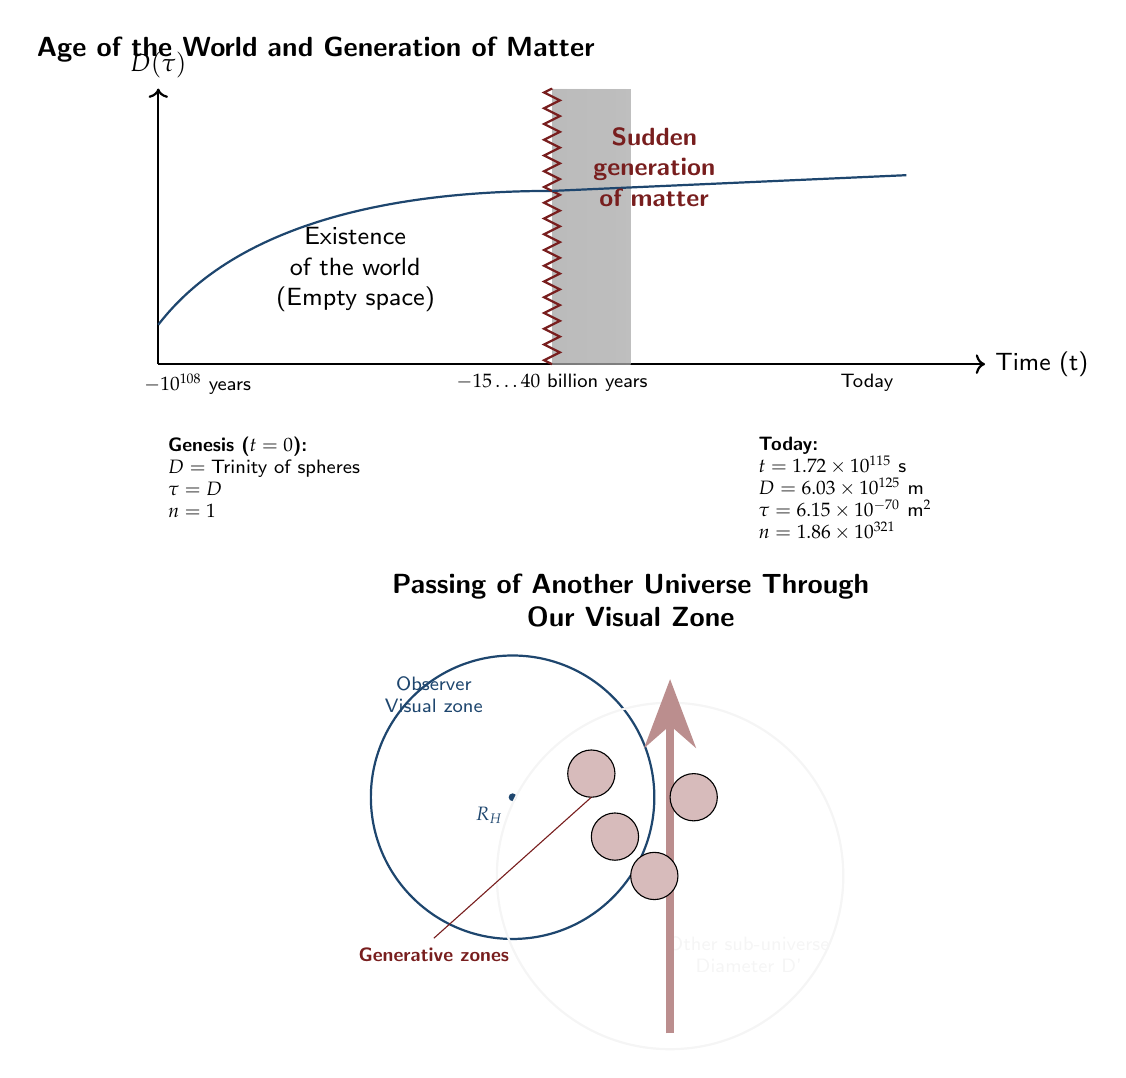
\begin{tikzpicture}

    % --- AGE OF WORLD GRAPH ---
    \node[font=\bfseries\sffamily, align=center] at (2, 4) {Age of the World and Generation of Matter};
    \begin{scope}[shift={(0, 0)}]
        \draw[->, thick] (0,0) -- (10.5,0) node[right, font=\sffamily\small] {Time (t)};
        \draw[->, thick] (0,0) -- (0,3.5) node[above, font=\sffamily\small] {$D(\tau)$};
        
        % The expansion curve
        \draw[thick, theoryblue] (0,0.5) .. controls (1,1.8) and (3,2.2) .. (5,2.2);
        
        % The Matter Generation Zone
        \fill[left color=theorygray!80, right color=white, opacity=0.5] (5,0) rectangle (6.0,3.5);
        \draw[thick, theoryred, decoration={zigzag, segment length=2mm, amplitude=1mm}, decorate] (5,0) -- (5,3.5);
        \draw[thick, theoryblue] (5,2.2) -- (9.5, 2.4); % Continued slight expansion
        
        \node[text width=3cm, align=center, font=\sffamily\small] at (2.5,1.2) {Existence of the world\\ (Empty space)};
        \node[text width=2cm, align=center, font=\sffamily\small, theoryred] at (6.3,2.5) {\textbf{Sudden\\ generation\\ of matter}};

        % Timeline labels
        \node[below, font=\sffamily\scriptsize] at (0.5,0) {$-10^{108}$ years};
        \node[below, font=\sffamily\scriptsize] at (5,0) {$-15 \dots 40$ billion years};
        \node[below, font=\sffamily\scriptsize] at (9,0) {Today};

        % Stat boxes
        \node[anchor=north west, align=left, font=\sffamily\scriptsize] at (0,-0.8) {
            \textbf{Genesis ($t=0$):}\\ $D = \text{Trinity of spheres}$\\ $\tau = D$\\ $n = 1$
        };
        \node[anchor=north west, align=left, font=\sffamily\scriptsize] at (7.5,-0.8) {
            \textbf{Today:}\\
            $t = 1.72 \times 10^{115}$ s \\ 
            $D = 6.03 \times 10^{125}$ m\\ 
            $\tau = 6.15 \times 10^{-70}$ m$^2$ \\
            $n = 1.86 \times 10^{321}$
        };
    \end{scope}

    % --- PASSING UNIVERSE DIAGRAM ---
    \begin{scope}[shift={(6, -6)}]
        \node[font=\bfseries\sffamily, align=center] at (0, 3) {Passing of Another Universe Through\\ Our Visual Zone};
        
        % Our Universe (Observer)
        \draw[thick, theoryblue] (-1.5, 0.5) circle (1.8); 
        \fill[theoryblue] (-1.5, 0.5) circle (0.05) node[below left, font=\sffamily\scriptsize] {$R_H$};
        \node[font=\sffamily\scriptsize, align=center, theoryblue] at (-2.5, 1.8) {Observer\\ Visual zone};
        
        % Other Universe
        \draw[thick, theorygray] (0.5, -0.5) circle (2.2); 
        \node[font=\sffamily\scriptsize, align=center, theorygray] at (1.5, -1.5) {Other sub-universe\\ Diameter D'};
        
        % Vector of movement
        \draw[-{Stealth[scale=1.5]}, theoryred!50, line width=3pt] (0.5,-2.5) -- (0.5, 2.0);
        
        % Generative zones (overlapping matter)
        \foreach \p in {(-0.5,0.8), (0.8,0.5), (0.3,-0.5), (-0.2, 0)}
            \draw[fill=theoryred!30] \p circle (0.3);
            
        \node[font=\sffamily\scriptsize, theoryred] (gz) at (-2.5, -1.5) {\textbf{Generative zones}};
        \draw[thin, theoryred] (gz.north) -- (-0.5, 0.5);
    \end{scope}

\end{tikzpicture}
\end{adjustbox}
\caption{Top: The timeline of cosmic expansion showing the sudden metronic shift that generated matter. Bottom: Because the total diameter $D$ is vastly larger than our visible Hubble radius $R_H$, it is geometrically possible for foreign sub-universes to transit our visual zone.}
\end{figure} 
\subsection{The Shrinking Metron and the Evolution of Time}

If $D$ and $\tau$ are linked, and the universe is observed to be expanding (as evidenced by cosmic redshift), then $\tau$ cannot be a static constant. Heim adopted the \textbf{Jordan-Dirac Hypothesis}, which posits that fundamental constants evolve over cosmic time. 

In Heim's cosmology:
\begin{enumerate}
    \item The number of Metrons ($n$) in the universe is strictly \textbf{increasing}.
    \item The area of the individual Metron ($\tau$) is strictly \textbf{shrinking} ($\frac{d\tau}{dt} < 0$).
    \item The overall diameter of the physical universe ($D$) is strictly \textbf{expanding} ($\frac{dD}{dt} > 0$).
\end{enumerate}

This leads to a profound philosophical and mathematical conclusion: \textbf{Time is not an independent axis; it is the process of metron division.} Time "flows" because the geometrical grain of the universe ($\tau$) is continually fracturing into smaller units. As the "pixels" of reality get smaller, the universe gains the capacity to hold more complex geometrical structures (particles, atoms, life).

\begin{table}[htbp]
\centering
\renewcommand{\arraystretch}{1.4}
\begin{tabular}{llll}
\toprule
\textbf{Parameter} & \textbf{State at $t=0$ (Genesis)} & \textbf{Evolution Process} & \textbf{State Today} \\
\midrule
\rowcolor{gray!10}
\textbf{Diameter $D$} & $D = \tau_0$ (Smallest possible) & Increasing via $\mu_3 = f(R_3)$ & $D \approx 6.03 \times 10^{125}$ m \\
\textbf{Metron $\tau$} & $\tau_0 \approx 43 \text{ m}^2$ (Maximum size) & Shrinking via $\mu_2 = f(T)$ & $\tau \approx 6.15 \times 10^{-70} \text{ m}^2$ \\
\rowcolor{gray!10}
\textbf{Number $n$} & $n = 1$ (A single "Pixel") & Increasing via $\mu_1 = f(S_2)$ & $n \approx 1.86 \times 10^{321}$ \\
\bottomrule
\end{tabular}
\caption{The cosmic evolution of the metron variables over time.}
\end{table}

\subsection{The Origin of the Universe: The Trinity of Spheres}
If we run the clock backward, $D$ shrinks and $\tau$ grows. However, $\tau$ cannot grow infinitely. The absolute beginning of time ($t=0$) occurs at the moment when a single Metron ($\tau_0$) covers the entire diameter of the primordial universe ($D_0$). At this exact limit:
\begin{equation}
    n = 1 \quad \implies \quad \tau_0 = \pi D_0^2
\end{equation}

When Heim substituted $\tau_0$ back into the 7th-degree Cosmological Equation, the function of the initial diameter $D_0$ resolved into a 7th-degree polynomial. As shown in Volume 2 (Eq. 47), Heim defined this as the \textbf{Genesis Equation}:
\begin{equation}
    \eta^7 - \eta = \pm a, \quad \text{where} \quad 2\eta^2 = f_{(0)} \sqrt[6]{6/\pi}, \quad a \sqrt{\pi} = \sqrt[6]{\pi/6}
\end{equation}

Solving this 7th-order algebraic equation for $\eta$ yields exactly \textbf{three real roots} ($y(\eta) = 0$). These roots correspond to the \textbf{3 distinct initial diameters} of the primordial universe at the absolute cosmic zero-point ($t=0$). 

\begin{figure}[htbp]
\centering
\begin{adjustbox}{max width=0.8\textwidth}
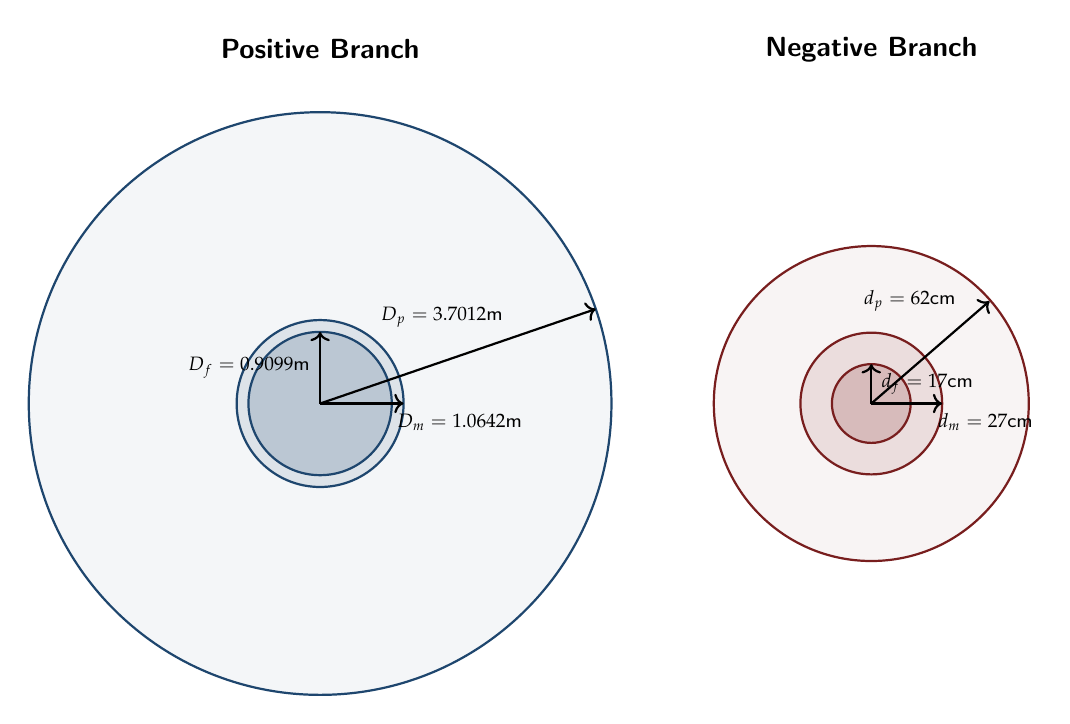
\begin{tikzpicture}
    % Positive Branch (Left)
    \node[font=\bfseries\sffamily] at (-3, 4.5) {Positive Branch};
    \draw[thick, theoryblue, fill=theoryblue!5] (-3, 0) circle (3.7);
    \draw[thick, theoryblue, fill=theoryblue!15] (-3, 0) circle (1.06);
    \draw[thick, theoryblue, fill=theoryblue!30] (-3, 0) circle (0.91);
    
    \draw[->, thick] (-3,0) -- (-3, 0.91) node[midway, left, font=\scriptsize\sffamily] {$D_f=0.9099$m};
    \draw[->, thick] (-3,0) -- (-1.94, 0) node[pos=0.8, below right, font=\scriptsize\sffamily] {$D_m=1.0642$m};
    \draw[->, thick] (-3,0) -- (0.5, 1.2) node[pos=0.7, above left, font=\scriptsize\sffamily] {$D_p=3.7012$m};

    % Negative Branch (Right)
    \node[font=\bfseries\sffamily] at (4, 4.5) {Negative Branch};
    \draw[thick, theoryred, fill=theoryred!5] (4, 0) circle (2.0); 
    \draw[thick, theoryred, fill=theoryred!15] (4, 0) circle (0.9);
    \draw[thick, theoryred, fill=theoryred!30] (4, 0) circle (0.5);
    
    \draw[->, thick] (4,0) -- (4, 0.5) node[midway, right, font=\scriptsize\sffamily] {$d_f=17$cm};
    \draw[->, thick] (4,0) -- (4.9, 0) node[pos=0.8, below right, font=\scriptsize\sffamily] {$d_m=27$cm};
    \draw[->, thick] (4,0) -- (5.5, 1.3) node[pos=0.8, above left, font=\scriptsize\sffamily] {$d_p=62$cm};
\end{tikzpicture}
\end{adjustbox}
\caption{The Trinity of Spheres (Fundamentalsphäre, Mesosphäre, Protosphäre). The primordial universe did not begin as a 0-dimensional singularity, but as two triples of monometric spheres resulting from the Genesis Equation.}
\end{figure}

\begin{mbbcite}
    \textbf{The Triple Structure of Time:} Heim argues that this "Trinity of Spheres" persists today as the fundamental structure of the "Present." A moment in time is not a zero-width slice, but is composed of three entangled actualizations (the $R_3$ metric, the $T$ metric, and the $S_2$ metric). 
\end{mbbcite}

\subsubsection{The Chronon (The Quantum of Time) and the Apeiron}
Because the physical space of the universe is quantized by the discrete Metron area ($\tau$), the expansion and evolution of the universe cannot occur smoothly. In Heim's cosmology, the universe updates in discrete, indivisible mathematical steps.

Heim defines the fundamental quantum of time as the \textbf{Chronon ($\vartheta$)}. The continuous time variable $t$ used in macroscopic physics is actually an illusion created by the rapid, sequential summation of Chronons. 
\begin{equation}
    t = n \cdot \vartheta \quad (\text{where } n \text{ is an integer})
\end{equation}

Heim identifies the fundamental "Present" as a geometric interval, not a zero-width point. He calls this the \textbf{Apeiron}. 
\begin{equation}
    T_0(D_{fmp}) = 0 \le t \le \vartheta(D_{pmf}) = 2 T_A < \infty
\end{equation}

During the open time interval ($0 < t < \vartheta$), the geometric state of the universe is "frozen" in the timeless background ($G_4$). When the Chronon step completes, the entire $R_6$ hyperstructure "actualizes" a new geometric state. Therefore, time is not a flowing river; it is the frame-by-frame projection of discrete geometric actualizations originating from the 12-dimensional background.

\subsubsection{The Chronon (The Quantum of Time)}
Because the physical space of the universe is quantized by the discrete Metron area ($\tau$), the expansion and evolution of the universe cannot occur smoothly. In Heim's cosmology, the universe updates in discrete, indivisible mathematical steps.

Heim defines the fundamental quantum of time as the \textbf{Chronon ($\vartheta$)}. The continuous time variable $t$ used in macroscopic physics is actually an illusion created by the rapid, sequential summation of Chronons. 
\begin{equation}
    t = n \cdot \vartheta \quad (\text{where } n \text{ is an integer})
\end{equation}

During the open time interval ($0 < t < \vartheta$), the geometric state of the universe is "frozen" in the timeless background ($G_4$). When the Chronon step completes, the entire $R_6$ hyperstructure "actualizes" a new geometric state. Therefore, time is not a flowing river; it is the frame-by-frame projection of discrete geometric actualizations originating from the 12-dimensional background.

\section{Holomorphisms and the Organization of Matter}
\label{sec:holomorphism}

\textit{References: Map "Development of life on earth" (Page 7)}

If the universe were driven solely by entropy (Axiom b), matter would rapidly degrade into a uniform, unstructured gas. Yet, the universe exhibits profound organization: atoms form molecules, molecules form cells, and cells form living organisms. 

Heim introduced the concept of the \textbf{Holomorphism}—a structural clasp or organizational template originating from the $S_2$ and $I_2$ dimensions. A holomorphism is not a physical force like gravity or electromagnetism. It is a teleological (goal-directed) geometric constraint. When multiple elementary structures (atoms/cells) interact in $R_3$, the background dimension $S_2$ projects a "clasp" over them, organizing them into a unified, higher-order structure sharing a single probability amplitude in $I_2$.

\subsection{Phylogenesis: Typostrophe vs. Typostasis}

This organizational model provides a radical geometric alternative to pure Neo-Darwinism. In the standard biological model, evolution is driven entirely by random mutations (a bottom-up process). However, the fossil record frequently displays periods of \textbf{Heavy Typogenesis} ("Typostrophe")—explosions of new, highly complex species appearing much faster than random mathematical probability should allow (e.g., the Cambrian Explosion). This is often followed by long periods of stagnation ("Typostasis").

\begin{figure}[htbp]
\centering
\begin{adjustbox}{max width=0.8\textwidth}
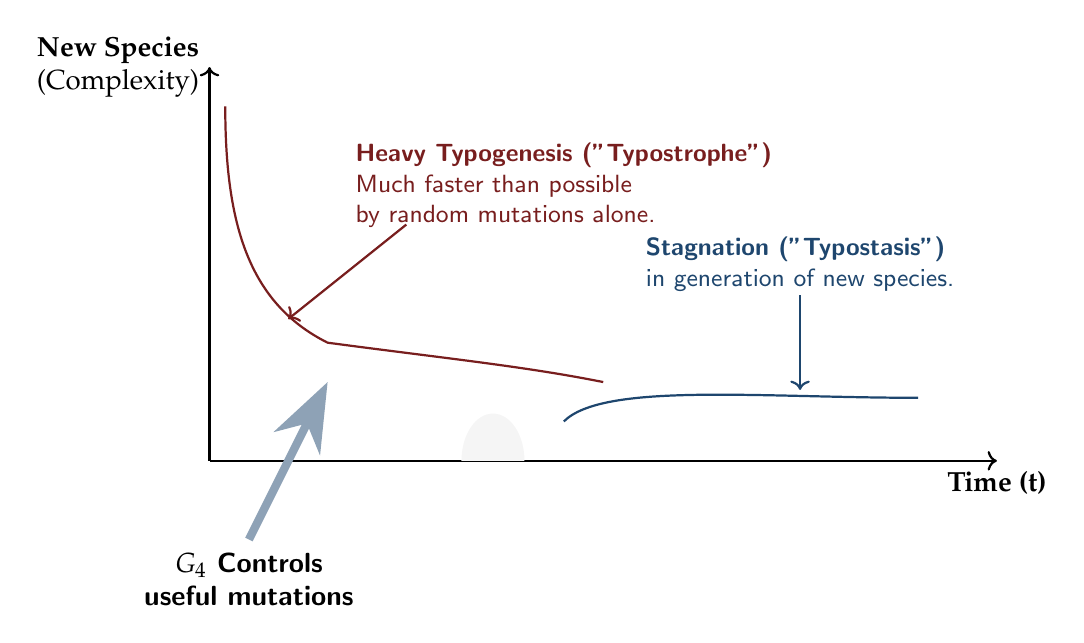
\begin{tikzpicture}
    % Axes
    \draw[->, thick] (0,0) -- (10,0) node[below] {\textbf{Time (t)}};
    \draw[->, thick] (0,0) -- (0,5) node[left, align=center] {\textbf{New Species}\\(Complexity)};
    
    % Typostrophe Curve
    \draw[thick, theoryred] (0.2, 4.5) .. controls (0.2, 3) and (0.5, 2) .. (1.5, 1.5) 
        .. controls (3, 1.3) and (4, 1.2) .. (5, 1);
        
    % Typostasis Curve
    \draw[thick, theoryblue] (4.5, 0.5) .. controls (5, 1) and (7, 0.8) .. (9, 0.8);

    % Annotations
    \node[font=\sffamily\small, align=left, theoryred] at (4.5, 3.5) {\textbf{Heavy Typogenesis ("Typostrophe")}\\ Much faster than possible\\ by random mutations alone.};
    \draw[->, thick, theoryred] (2.5, 3) -- (1.0, 1.8);
    
    \node[font=\sffamily\small, align=left, theoryblue] at (7.5, 2.5) {\textbf{Stagnation ("Typostasis")}\\ in generation of new species.};
    \draw[->, thick, theoryblue] (7.5, 2.1) -- (7.5, 0.9);

    % The G4 control arrow
    \fill[theorygray] (4.0,0) arc(0:180:0.4 and 0.6); 
    \draw[-{Stealth[scale=1.5]}, line width=3pt, theoryblue!50] (0.5,-1) -- (1.5, 1.0);
    \node[font=\sffamily\bfseries, align=center] at (0.5, -1.5) {$G_4$ Controls\\ useful mutations};

\end{tikzpicture}
\end{adjustbox}
\caption{The phylogenesis of species in Heim theory. Evolutionary leaps are driven by top-down $G_4$ holomorphism projections, not just bottom-up random mutation.}
\end{figure}

In Heim Theory, these evolutionary leaps are not random. They are the result of \textbf{$G_4$ controlling useful mutations}. When the environmental conditions in $R_3$ are suitable, the timeless background ($G_4$) projects a new, more complex Holomorphism down through $S_2$, physically clasping existing genetic material into a higher-order structure. 

\subsection{The Hierarchy of Holomorphisms}

These holomorphisms exist in a strict hierarchy, originating from the "Asomaton" (the elementary $G_4$ structure of intent). The Asomaton represents pure organizational intent, which projects downwards through Information ($I_2$) and Structure ($S_2$) to act as a "bracket" over physical matter in $R_4$:

\begin{enumerate}
    \item \textbf{Lower Holomorphisms (Substructures):} Organize atoms into complex molecules, and molecules into living cells.
    \item \textbf{Standard Holomorphisms:} Organize cells into complex, multicellular organisms (plants, animals, humans).
    \item \textbf{Superordinated Holomorphisms:} The highest level of organizational clasping, responsible for state-building and collective behaviors in advanced species (e.g., ant colonies or human societies).
\end{enumerate}

\begin{figure}[htbp]
\centering
\begin{adjustbox}{max width=\textwidth}
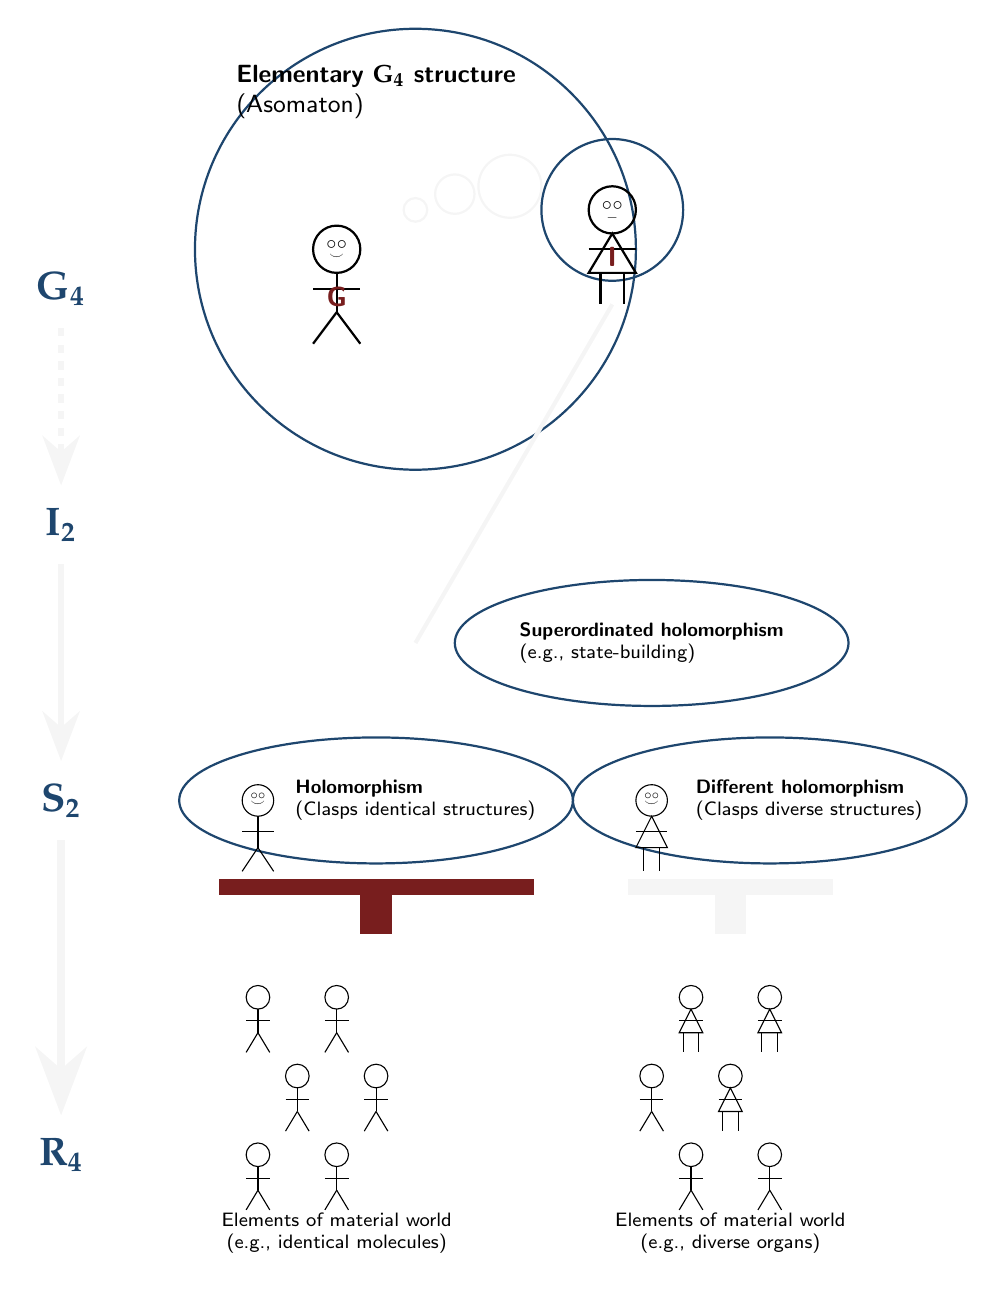
\begin{tikzpicture}[
    node distance=0.4cm,
    arrow/.style={-{Stealth[scale=1.5]}, line width=2pt, theorygray},
    dashedarrow/.style={-{Stealth[scale=1.5]}, dashed, line width=2pt, theorygray}
]

    % The Left G4 -> I2 -> S2 -> R4 Axis
    \begin{scope}[shift={(-6,0)}]
        \node[font=\Large\bfseries\sffamily, theoryblue] (g4) at (0,0) {$\mathbf{G_4}$};
        \draw[dashedarrow] (0,-0.5) -- (0,-2.5);
        \node[font=\Large\bfseries\sffamily, theoryblue] (i2) at (0,-3) {$\mathbf{I_2}$};
        \draw[arrow] (0,-3.5) -- (0,-6);
        \node[font=\Large\bfseries\sffamily, theoryblue] (s2) at (0,-6.5) {$\mathbf{S_2}$};
        \draw[arrow, line width=3pt] (0,-7) -- (0,-10.5);
        \node[font=\Large\bfseries\sffamily, theoryblue] (r4) at (0,-11) {$\mathbf{R_4}$};
    \end{scope}
    
    % Main Central Graphic Area
    \begin{scope}[shift={(0,0)}]
        
        % G4 Level Circle (Asomaton)
        \draw[theoryblue, thick] (-1.5, 0.5) circle (2.8cm);
        \node[font=\sffamily\small, align=left] at (-2, 2.5) {\textbf{Elementary $\mathbf{G_4}$ structure}\\ (Asomaton)};
        
        % Asomaton figure 1 (G4)
        \begin{scope}[shift={(-2.5, 0.5)}]
            \draw[thick] (0,0) circle (0.3); % Head
            \node[font=\scriptsize] at (0,0.05) {$\circ\circ$}; \node[font=\tiny] at (0,-0.1) {$\smile$};
            \draw[thick] (0,-0.3) -- (0,-0.8); % Body
            \draw[thick] (-0.3,-0.5) -- (0.3,-0.5); % Arms
            \draw[thick] (0,-0.8) -- (-0.3,-1.2); \draw[thick] (0,-0.8) -- (0.3,-1.2); % Legs
            \node[font=\sffamily\bfseries, theoryred] at (0, -0.6) {G};
        \end{scope}
        
        % Thought bubbles
        \draw[thick, theorygray] (-1.5, 1) circle (0.15); 
        \draw[thick, theorygray] (-1.0, 1.2) circle (0.25); 
        \draw[thick, theorygray] (-0.3, 1.3) circle (0.4);
        
        % Asomaton figure 2 (I2) inside smaller circle
        \begin{scope}[shift={(1.0, 1)}]
            \draw[theoryblue, thick] (0,0) circle (0.9);
            \draw[thick] (0,0) circle (0.3); % Head
            \node[font=\scriptsize] at (0,0.05) {$\circ\circ$}; \node[font=\tiny] at (0,-0.1) {$-$};
            \draw[thick] (-0.3,-0.8) -- (0.3,-0.8) -- (0,-0.3) -- cycle; % Triangle Body
            \draw[thick] (-0.3,-0.5) -- (0.3,-0.5); % Arms
            \draw[thick] (-0.15,-0.8) -- (-0.15,-1.2); \draw[thick] (0.15,-0.8) -- (0.15,-1.2); % Legs
            \node[font=\sffamily\bfseries, theoryred] at (0, -0.6) {I};
        \end{scope}

        % Diagonal Connection down to S2
        \draw[thick, theorygray, line width=1.5pt] (1.0, -0.2) -- (-1.5, -4.5);

        % Superordinated Holomorphism
        \draw[theoryblue, thick] (1.5, -4.5) ellipse (2.5cm and 0.8cm);
        \node[font=\sffamily\scriptsize, align=left] at (1.5, -4.5) {\textbf{Superordinated holomorphism}\\ (e.g., state-building)};
        
        % Left S2 Circle (Same structural design)
        \draw[theoryblue, thick] (-2, -6.5) ellipse (2.5cm and 0.8cm);
        \begin{scope}[shift={(-3.5, -6.5)}]
            \draw (0,0) circle (0.2); \node[font=\tiny] at (0,0.05) {$\circ\circ$}; \node[font=\tiny] at (0,-0.05) {$\smile$};
            \draw (0,-0.2) -- (0,-0.6); \draw (-0.2,-0.4) -- (0.2,-0.4); 
            \draw (0,-0.6) -- (-0.2,-0.9); \draw (0,-0.6) -- (0.2,-0.9);
        \end{scope}
        \node[font=\sffamily\scriptsize, align=left] at (-1.5, -6.5) {\textbf{Holomorphism}\\ (Clasps identical structures)};
        
        % Right S2 Circle (Different holomorphism)
        \draw[theoryblue, thick] (3, -6.5) ellipse (2.5cm and 0.8cm);
        \begin{scope}[shift={(1.5, -6.5)}]
            \draw (0,0) circle (0.2); \node[font=\tiny] at (0,0.05) {$\circ\circ$}; \node[font=\tiny] at (0,-0.05) {$\smile$};
            \draw (-0.2,-0.6) -- (0.2,-0.6) -- (0,-0.2) -- cycle; \draw (-0.2,-0.4) -- (0.2,-0.4);
            \draw (-0.1,-0.6) -- (-0.1,-0.9); \draw (0.1,-0.6) -- (0.1,-0.9);
        \end{scope}
        \node[font=\sffamily\scriptsize, align=left] at (3.5, -6.5) {\textbf{Different holomorphism}\\ (Clasps diverse structures)};

        % Bracket connecting S2 to R4 (Left side)
        \fill[theoryred] (-4, -7.5) rectangle (0, -7.7);
        \fill[theoryred] (-2.2, -7.7) rectangle (-1.8, -8.2);
        
        % Bracket connecting S2 to R4 (Right side)
        \fill[theorygray] (1.2, -7.5) rectangle (3.8, -7.7);
        \fill[theorygray] (2.3, -7.7) rectangle (2.7, -8.2);

        % --- R4 Level Elements (Left Group - Identical) ---
        \begin{scope}[shift={(-2, -9)}]
            \foreach \x/\y in {-1.5/0, -0.5/0, -1/-1, 0/-1, -1.5/-2, -0.5/-2} {
                \begin{scope}[shift={(\x, \y)}]
                    \draw (0,0) circle (0.15); \draw (0,-0.15) -- (0,-0.45); \draw (-0.15,-0.3) -- (0.15,-0.3); 
                    \draw (0,-0.45) -- (-0.15,-0.7); \draw (0,-0.45) -- (0.15,-0.7);
                \end{scope}
            }
        \end{scope}
        \node[font=\sffamily\scriptsize, align=center] at (-2.5, -12.0) {Elements of material world\\ (e.g., identical molecules)};

        % --- R4 Level Elements (Right Group - Diverse) ---
        \begin{scope}[shift={(3.5, -9)}]
            \foreach \x/\y in {-1.5/0, -0.5/0, -1/-1} { % Triangles
                \begin{scope}[shift={(\x, \y)}]
                    \draw (0,0) circle (0.15); \draw (-0.15,-0.45) -- (0.15,-0.45) -- (0,-0.15) -- cycle; 
                    \draw (-0.15,-0.3) -- (0.15,-0.3); \draw (-0.1,-0.45) -- (-0.1,-0.7); \draw (0.1,-0.45) -- (0.1,-0.7);
                \end{scope}
            }
            \foreach \x/\y in {-2/-1, -1.5/-2, -0.5/-2} { % Stickmen
                \begin{scope}[shift={(\x, \y)}]
                    \draw (0,0) circle (0.15); \draw (0,-0.15) -- (0,-0.45); \draw (-0.15,-0.3) -- (0.15,-0.3); 
                    \draw (0,-0.45) -- (-0.15,-0.7); \draw (0,-0.45) -- (0.15,-0.7);
                \end{scope}
            }
        \end{scope}
        \node[font=\sffamily\scriptsize, align=center] at (2.5, -12.0) {Elements of material world\\ (e.g., diverse organs)};

    \end{scope}
\end{tikzpicture}
\end{adjustbox}
\caption{The Chain of Effects: Teleological intent (Asomaton) in $G_4$ translates to information amplitudes in $I_2$, which form organizational "clasps" (Holomorphisms) in $S_2$. These clasps bind the physical matter of $R_4$ together into complex organisms.}
\end{figure}

\begin{tcolorbox}[colback=white, colframe=theoryred, title=\textbf{Conclusion of the $R_{12}$ Framework}]
Life is not an accident of chemistry in a dying, entropic universe. Life is the direct, structural manifestation of the $G_4$ and $I_2$ dimensions organizing the metron grid. As the Metron ($\tau$) shrinks over cosmic time (Chapter 6), the "resolution" of the universe increases, allowing the $R_6$ material world to support increasingly complex Holomorphisms. The universe is, fundamentally, a geometry designed to evolve consciousness.
\end{tcolorbox}
\section{Beyond the Continuum: The Metronization of Area}
\label{sec:metron_calculus}

\textit{References: Fundamental Structure, Volume 1, Chapter 3; Metron Basic Operations}

The establishment of the Metron ($\tau \approx 6.15 \times 10^{-70} \text{ m}^2$) as a fundamental, non-zero geometric unit of area forces a radical paradigm shift in mathematical physics. In standard calculus, the foundational operation is the infinitesimal limit ($dx \to 0$). However, in Heim Theory, because space cannot be divided into units smaller than $\tau$, the infinitesimal limit is physically invalid. 

\textbf{The continuum does not exist in the microscopic world.} Consequently, the differential equations of General Relativity and Quantum Mechanics are merely macroscopic approximations. To accurately describe the interactions of elementary particles, continuous mathematics must be replaced by a discrete difference calculus operating on a 6-dimensional integer grid.

\subsection{Quantization of the Definite Integral}

In standard continuous calculus, the definite integral of a function $f(x)$ represents the exact area under the curve. In a metronized space, this area must be an exact \textbf{integer multiple} of the fundamental unit $\tau$. If we divide the area into $n$ discrete intervals, the integral is replaced by:
\begin{equation}
    \int_{x_0}^{x_n} f(x)dx = n\tau \quad \text{(where $n \in \mathbb{Z}^+$)}
\end{equation}

In this interpretation, the continuous coordinates $x$ and continuous function values $y = f(x)$ are replaced by sequences of integers. The distance between any two points is not a smooth line, but a count of the number of metrons separating them:
\begin{equation}
    x_n = x(n), \quad y_n = f(x_n) = f(n)
\end{equation}

\begin{figure}[htbp]
\centering
\begin{adjustbox}{max width=0.65\textwidth}
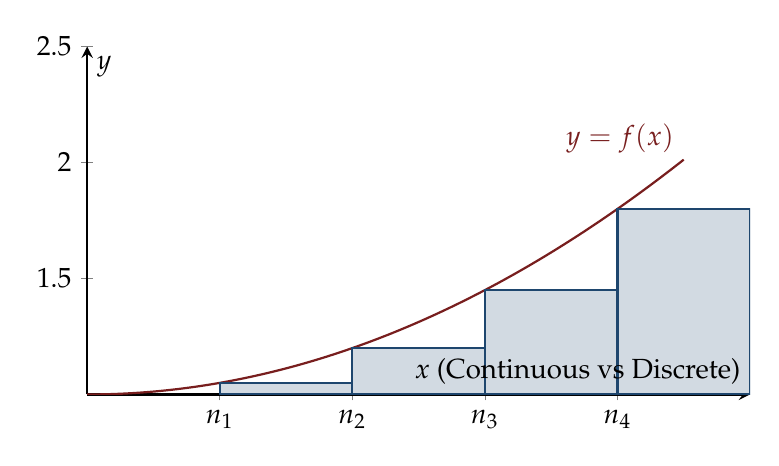
\begin{tikzpicture}
    \begin{axis}[
        axis lines = middle,
        xlabel = $x$ (Continuous vs Discrete),
        ylabel = $y$,
        xtick = {1, 2, 3, 4},
        xticklabels = {$n_1$, $n_2$, $n_3$, $n_4$},
        ymax = 2.5,
        xmax = 5,
        width = 10cm, height = 6cm,
        axis line style={thick},
        tick label style={font=\sffamily}
    ]
    % Continuous curve
    \addplot [domain=0:4.5, samples=100, thick, theoryred] {1 + 0.05*x^2};
    \node[theoryred, anchor=south east] at (axis cs: 4.5, 2.0) {$y = f(x)$};

    % Discrete Metron blocks
    \addplot [ybar interval, fill=theoryblue!20, draw=theoryblue, thick] coordinates {(1,1.05) (2,1.2) (3,1.45) (4,1.8) (5, 2.25)};
    
    \node[font=\Large\bfseries\sffamily, theoryblue] at (axis cs: 1.5, 0.5) {$\tau$};
    \node[font=\Large\bfseries\sffamily, theoryblue] at (axis cs: 2.5, 0.6) {$\tau$};
    \node[font=\Large\bfseries\sffamily, theoryblue] at (axis cs: 3.5, 0.72) {$\tau$};
    \node[font=\Large\bfseries\sffamily, theoryblue] at (axis cs: 4.5, 0.9) {$\tau$};
    \end{axis}
\end{tikzpicture}
\end{adjustbox}
\caption{Discrete metronization of space. The continuous integral (red curve) is a macroscopic approximation of the true physical reality, which consists of discrete geometric area quanta $\tau$ (blue blocks).}
\end{figure}

\subsection{Vacuum Energy and Cosmological Inflation}
To explain how matter was initially generated in the empty expanding metron grid, Heim and Dröscher modeled the early universe's vacuum energy ($M'_v$). 

Dröscher utilized the analogy of a spring stretched between two mounts. If the center of the spring is displaced, one side is compressed and the other stretched, creating two distinct potential energies ($M'_1$ and $M'_2$). When the universe was in its primordial state, a rapid shift in the metron grid released immense potential energy from the vacuum. 

Heim calculates that this vacuum energy spontaneously generated ultra-heavy elementary masses (equivalent to the hypothesized $X$-Bosons, with masses around $10^{15} \text{ GeV}$). These particles were highly unstable and decayed almost instantly. This rapid decay released massive amounts of secondary particles and energy, causing a rapid geometric expansion of the $R_3$ space. Heim's purely geometric derivation perfectly mirrors the modern astrophysical concept of \textbf{Cosmological Inflation}, explaining how the early universe filled with the Baryons and Mesons we observe today.

\section{The Rules of Metron Calculus (\texorpdfstring{$\ethop$}{eth})}

Because the domain variables $n$ are integers, Heim introduces a new operator for differentiation, denoted by the Icelandic letter \textbf{eth} ($\ethop$). When $\ethop$ appears, it signifies that the operation is a discrete step on an integer sequence.

\subsection{Metron Differentiation}

The continuous derivative $\frac{df}{dx} = \lim_{\Delta x \to 0} \frac{f(x+\Delta x) - f(x)}{\Delta x}$ is replaced. The smallest possible step size in the metron grid is $\Delta n = 1$. Therefore, the metron derivative of a state function $\varphi(n)$ is strictly defined as the difference between the current state and the adjacent previous state:
\begin{equation}
    \frac{\ethop \varphi}{\ethop n} = \lim_{\nu \to +1} \frac{1}{\nu}(\varphi(n) - \varphi(n-\nu)) = \varphi(n) - \varphi(n-1)
\end{equation}
Since $\ethop n = 1$, the standard notation becomes:
\begin{equation}
    \ethop \varphi(n) = \varphi(n) - \varphi(n-1) \quad (\text{for } 1 \le n \le N)
\end{equation}

This operation possesses a \textbf{Projective Property}: with each derivation, the available domain of the function narrows by one. If $\varphi$ is defined on $[0, N]$, $\ethop \varphi$ is defined on $[1, N]$, and $\ethop^2 \varphi$ is defined on $[2, N]$. This prevents the infinite recursions found in continuous mathematics.

\subsection{Metron Integration (\texorpdfstring{$S$}{S})}

The inverse operation is metron integration, denoted by $S$ (summation) rather than the integral symbol $\int$. If $\varphi = \ethop \phi$, then:
\begin{equation}
    S_{n_1}^{n_2} \varphi \, \ethop n = S_{n_1}^{n_2} \ethop \phi = \sum_{n=n_1}^{n_2} (\phi(n) - \phi(n-1)) = \phi(n_2) - \phi(n_1-1)
\end{equation}

\textbf{Crucial Departure from the Continuum:} In continuous calculus, the integral of a point is zero ($\int_a^a f(x)dx = 0$). However, in Metron calculus, the integral over a single metron interval evaluates to the function value itself:
\begin{equation}
    S_{n_1}^{n_1} \varphi \, \ethop n = \phi(n_1) - \phi(n_1 - 1) = \ethop \phi(n_1) = \varphi(n_1) \neq 0
\end{equation}
This is the mathematical mechanism that entirely prevents point-singularities (like black holes or infinite charge densities) in Heim Theory. Energy cannot be compressed into a zero-volume point because the smallest possible integral evaluates to a finite area ($\tau$).

\begin{tcolorbox}[colback=white, colframe=theoryblue, title=\textbf{Key Rules of Metron Calculus}]
\begin{itemize}
    \item \textbf{Constant Rule:} $\ethop C = 0$
    \item \textbf{Product Rule:} $\ethop (uv) = u \ethop v + v \ethop u - \ethop u \ethop v$
    \item \textbf{Higher-Order Differential (Binomial Expansion):} $\displaystyle \ethop^k \varphi = \sum_{\nu=0}^{k} (-1)^\nu \binom{k}{\nu} \varphi(n-\nu)$
    \item \textbf{Quotient Rule:} $\ethop \left( \frac{u}{v} \right) = \frac{1}{v} \begin{vmatrix} \ethop u & \ethop v \\ u & v \end{vmatrix} \cdot \begin{vmatrix} v & \ethop v \\ 1 & 1 \end{vmatrix}^{-1}$
    \item \textbf{Quotient Integral:} $\displaystyle S \frac{\varphi}{\Psi} \ethop n = \frac{u}{v}, \quad \text{where } \frac{\varphi}{\Psi} = \frac{v \ethop u - u \ethop v}{v(n)v(n-1)}$
    \item \textbf{Partial Integration:} $S u \ethop v = uv - S (v - \ethop v) \ethop u$
    \item \textbf{Macroscopic Exponential Approx:} $\ethop_\epsilon e^\varphi \approx e^\varphi \ethop_\epsilon \varphi$ (Valid only when $\tau$ is extremely small relative to the macroscopic scale).
\end{itemize}
\end{tcolorbox}

\section{Selector Theory: The Operators of Discrete Geometry}
\label{sec:selector_theory}

With the mathematical tools of discrete difference calculus established, Heim transitions from simple calculus to \textbf{Operator Theory}. In a discrete integer space, geometry is not defined by continuous stretching or curving; it is defined by \textit{selecting} adjacent coordinate states.

Heim defines the metron derivative as a \textbf{Selector Operator}, denoted by $C$. When $C$ acts on a metron function $\varphi$, it selects the geometric difference. Heim uses a semicolon ($;$) to denote the application of a selector to a state:
\begin{equation}
    C; \varphi(n) = \ethop \varphi(n) = \varphi(n) - \varphi(n-1)
\end{equation}

\subsection{Types of Selectors}

Every geometric state in the $R_6$ hyperstructure can be expressed as a sequence of selectors acting on positive integer metron numbers ($n_i$).

\begin{enumerate}
    \item \textbf{Assignment Selectors (\textit{Zuordnungsselektors}):} Select a specific dimensional component. $Z(i); n = n_i$.
    \item \textbf{Function Selectors:} Represent complex mathematical operations (like differentiation or geometric twisting). $\varphi(n_i)_1^L = \phi; n$.
    \item \textbf{Identity Selector:} Leaves the metron state unchanged. $E; n = 1$, and $E; (\ ); n = n$.
\end{enumerate}

\subsection{Metron Tensors and Non-Commutativity}

To build a unified field theory, Heim must reconstruct the metric tensor ($g_{ik}$) using these selectors. In $L$ dimensions, an Assignment Selector is given an orientation (a direction $\bar{e}_i$), becoming an \textbf{Oriented Assignment Selector} $\bar{Z}(i)$:
\begin{equation}
    \bar{Z}(i) = \bar{e}_i (\ )_i, \quad (\bar{e}_i, \bar{e}_k)_L = \hat{A}(n_i)_1^L
\end{equation}
Here, $\hat{A}$ is the \textbf{Orientation Matrix}. If $\hat{A}$ is the identity matrix, the discrete space is perfectly flat and orthogonal. If $\hat{A}$ varies with $n_i$, the space is curved.

By multiplying these directed selectors together, Heim generates \textbf{Metron Tensors} of order $m$:
\begin{equation}
    {}^m \bar{T} = {}^m \bar{C}; n = \left( \prod_{k=1}^m C_{i_k} \right); n
\end{equation}

\begin{figure}[htbp]
\centering
\begin{adjustbox}{max width=0.7\textwidth}
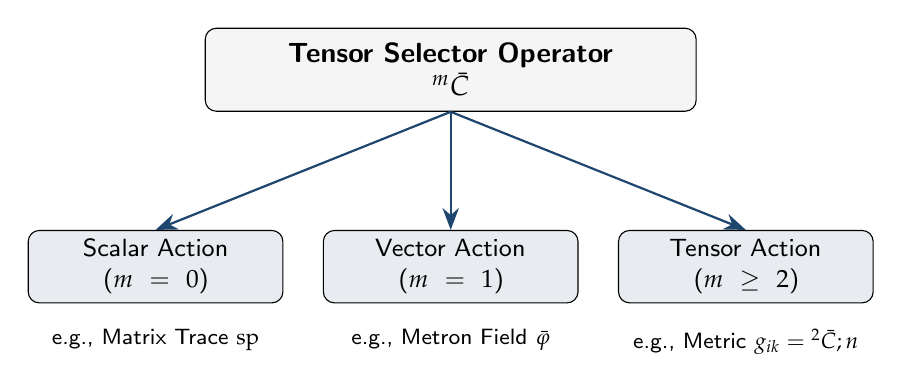
\begin{tikzpicture}[
    node distance=0.6cm,
    process/.style={rectangle, draw, fill=theoryblue!10, rounded corners, minimum height=2.5em, text width=3cm, text centered, font=\sffamily\small},
    arrow/.style={-{Stealth[scale=1.2]}, thick, theoryblue}
]
    \node[rectangle, draw, fill=theorygray, rounded corners, minimum height=3em, text width=6cm, text centered, font=\sffamily\bfseries] (selector) {Tensor Selector Operator\\${}^m \bar{C}$};
    
    \node[process, below left=1.5cm and -1cm of selector] (scalar) {Scalar Action\\($m=0$)};
    \node[process, below=1.5cm of selector] (vector) {Vector Action\\($m=1$)};
    \node[process, below right=1.5cm and -1cm of selector] (tensor) {Tensor Action\\($m \ge 2$)};

    \draw[arrow] (selector.south) -- (scalar.north);
    \draw[arrow] (selector.south) -- (vector.north);
    \draw[arrow] (selector.south) -- (tensor.north);
    
    \node[font=\footnotesize\sffamily, below=0.2cm of scalar] {e.g., Matrix Trace $\spn$};
    \node[font=\footnotesize\sffamily, below=0.2cm of vector] {e.g., Metron Field $\bar{\varphi}$};
    \node[font=\footnotesize\sffamily, below=0.2cm of tensor] {e.g., Metric $g_{ik} = {}^2 \bar{C}; n$};

\end{tikzpicture}
\end{adjustbox}
\caption{The hierarchical generation of geometric structures in $R_6$ using Tensor Selectors.}
\end{figure}

\textbf{The Origin of Physical Fields:} A fundamental algebraic property of Selectors is that \textbf{they do not commute under multiplication}. 
\begin{equation}
    (C_i \times C_k)_{\pm} \neq 0 \implies C_i C_k - C_k C_i \neq 0
\end{equation}

When constructing the second-order tensor selector ${}^2 \bar{C}$ (which generates the metric $g_{ik}$), this non-commutativity naturally splits the metric into two parts:
\begin{equation}
    {}^2 \bar{C} = {}^2 \bar{C}_+ + {}^2 \bar{C}_-
\end{equation}
Where ${}^2 \bar{C}_+$ is symmetric (Hermitian) and ${}^2 \bar{C}_-$ is antisymmetric (anti-Hermitian). 

This is the exact mathematical mechanism that justifies the equivalence approach established in Chapter 3. The symmetric selector (${}^2 \bar{C}_+$) generates the gravitational field, while the antisymmetric, non-commutative selector (${}^2 \bar{C}_-$) generates the electromagnetic field. The fields are not distinct physical substances; they are simply the symmetric and antisymmetric byproducts of multiplying discrete geometric operators in a 6-dimensional space.

\subsection{Example: The Fibonacci Construction Selector}
To understand how a discrete geometry "selects" a stable state, Heim uses the Fibonacci sequence ($\varphi(n) = \varphi(n-1) + \varphi(n-2)$) as a metron function. 

By applying the metron derivative ($\ethop\varphi = \varphi(n) - \varphi(n-1)$) twice, Heim derives the corresponding \textbf{Construction Selector} equation:
\begin{equation}
    \ethop^2 \varphi - 3\ethop\varphi + \varphi = 0 \quad \implies \quad (\ethop^2 - 3\ethop + E); \varphi = 0
\end{equation}
Just as this discrete operator naturally selects the golden ratio limits ($2\xi = 1 \pm \sqrt{5}$) from an infinite field of integers, the World Selector of $R_6$ selects the stable mass states of elementary particles from the geometric void. 

\subsection{Metron Spin and the Origin of Vector Potential}

Because the fundamental geometric unit ($\tau$) is a 2-dimensional area, every metron inherently possesses a boundary loop. The metron derivative of two independent geodesics ($\bar{\xi}_\alpha, \bar{\xi}_\beta$) enclosing this area results in a tensor quantity representing rotation. 

Heim defines this geometric rotation as the \textbf{Metron Spin Matrix ($\hat{s}$)}:
\begin{equation}
    \hat{s} = \operatorname{ROT}_N \hat{\phi} = \begin{pmatrix} 0 & {}^2\bar{s}_{12} \\ -{}^2\bar{s}_{12} & 0 \end{pmatrix}, \quad \text{where } {}^2\bar{s}_{\alpha\beta}; n = S S \ethop\bar{\xi}_\alpha \times \ethop\bar{\xi}_\beta
\end{equation}
This spin represents the "preformation of space." The area units of the universe are not static squares; they possess an internal rotational degree of freedom. 

\begin{mbbcite}
    \textbf{The True Nature of Vector Potential:} In classical electromagnetism, magnetic fields are described by the curl of a Vector Potential ($\vec{B} = \operatorname{rot}\vec{A}$). Heim theory reveals that this continuous vector potential is actually an illusion. The vector potential is simply the macroscopic statistical interpretation of the discrete metron spin selectors acting on the boundary loops of the fundamental area quanta.
\end{mbbcite}
\subsection{Metron Vector Analysis Analogies}

To ensure that macroscopic physics emerges smoothly from this discrete foundation, Heim established metronic equivalents for standard vector calculus operations ($\operatorname{div}, \operatorname{rot}, \operatorname{grad}$):

\begin{align}
    \text{Gradient:} \quad \bar{\ethop} \varphi &= \mathrm{GRAD_L} \varphi \\
    \text{Divergence:} \quad \spn \bar{\ethop}; {}^m \bar{C} &= \overline{\mathrm{DIV_L}} {}^m \bar{C} \\
    \text{Rotation (Curl):} \quad \bar{\ethop}; {}^m \bar{C} - (\bar{\ethop}; {}^m \bar{C})^x &= \mathrm{ROT_L} {}^m \bar{C}
\end{align}

These discrete operators maintain the familiar null-identities of classical physics (e.g., $\mathrm{DIV_L} \mathrm{ROT_L} = 0$ and $\mathrm{ROT_L} \mathrm{GRAD_L} = {}^2 0$), proving that Maxwell's equations and Newton's laws are perfectly preserved as the large-scale statistical averages of these underlying discrete selector operations. 

Specifically, the metronic counterpart to Gauss's Divergence Theorem ($\iiint \operatorname{div} \vec{A} dV = \iint \vec{A} \cdot dS$) is perfectly preserved across $L$-dimensional hyper-volumes:
\begin{equation}
    S_{\Omega(L)} \mathrm{DIV_L} \bar{\phi} \ethop V = S_{\Omega(L-1)} \bar{\phi} \ethop \bar{V}
\end{equation}
\section{From Continuous Geometry to Metronic Hyperstructure}
\label{sec:polymetric_condensation}

\textit{References: Metron Calculations (Parts 10-13); Elementarstrukturen der Materie 1, Chapter 4; Map III-2}

The previous chapters established that the physical universe is a 6-dimensional discrete manifold ($R_6$), quantized by the Metron area ($\tau$), and governed by discrete difference operators (Selectors). The ultimate goal of Heim Theory is to derive the properties of matter directly from this geometry. 

To achieve this, Heim must answer the fundamental question: \textit{How does "empty" space compress and twist to form a particle?}

In General Relativity, the curvature of space-time is defined by the metric tensor $g_{ik}$ and its derivatives, compiled into the Christoffel symbols (the affine connections). Heim takes this continuous formalism and translates it into a discrete **Metronic Hyperstructure**. 

\subsection{The Fundamental Condensor (Lattice Kernel)}

If space is a grid of metrons, then curvature is simply a change in the density of these metrons. Heim defines this "structural condensation" mathematically using a coefficient vector $\bar{K}$, which represents the density change across the grid:
\begin{equation}
    \underline{N} = S \bar{K} \ethop \bar{n}
\end{equation}
Where $S$ is the metron integral (summation) and $\bar{n}$ is the metron number vector. 

Heim relates this condensation vector $\bar{K}$ directly to the \textbf{Lattice Kernel} (${}^2 \bar{\kappa}$):
\begin{equation}
    {}^2 \bar{K} = {}^2 \bar{\kappa}; n
\end{equation}
The Lattice Kernel is the operator that generates the metric tensor itself:
\begin{equation}
    {}^2 \bar{\gamma} = \spn({}^2 \bar{\kappa} \times {}^2 \bar{\kappa})
\end{equation}
When the kernel ${}^2 \bar{\kappa}$ is the identity matrix, the metron grid is uniform, and the space is "flat" and empty. When the kernel deviates from identity, the metrons are "condensed"—this is what we perceive macroscopically as gravitational or electromagnetic fields.

Because the fundamental metron $\tau$ is a 2-dimensional area ($p=2$), a simple 1-dimensional number line cannot exist. The number of independent simple metron tensors $L$ that can exist in a space of dimension $N$ is dictated by the binomial relationship:
\begin{equation}
    L = \binom{N}{p} \quad \text{and} \quad \frac{N}{p} = M \ge 1 \text{ (where } M \in \mathbb{Z} \text{)}
\end{equation}
For our 4-dimensional space-time ($N=4, p=2$), this yields exactly $L = \binom{4}{2} = 6$. This provides a secondary, purely combinatorial proof that the quantization of area mandates a 6-dimensional coordinate representation.
\subsection{Metronizing the Affine Connections}

In continuous geometry, the Christoffel symbol of the first kind ($\Gamma_{akj}$) describes how basis vectors change as you move through curved space. Heim metronizes this concept by replacing the continuous derivative with the \textbf{Fundamental Condensor} (also called the \textit{Elementary Capacitor}).

Because the Lattice Kernel contains both symmetric (Hermitian) and antisymmetric (non-Hermitian) parts representing gravity and electromagnetism respectively (${}^2 \bar{\kappa} = {}^2 \bar{\kappa}_+ + {}^2 \bar{\kappa}_-$), the resulting discrete connection must also handle these dual structures.

Heim defines the discrete equivalent of the Christoffel symbol as the \textbf{Elementary Capacitor} $[\widehat{ab}]$:
\begin{equation}
    \Gamma_{pkl}^{(ab)}(\tau) = \metroncap{ }{pkl}{(ab)}; n, \quad {}^{[3]}\metroncap{ }{pkl}{(ab)} = [\widehat{ab}]
\end{equation}

To raise the indices and form the Christoffel symbol of the second kind ($\Gamma^i_{kj}$), Heim uses the inverse metric selector, creating a "binary elementary capacitor" that links the polymetric substructures:
\begin{equation}
    \gamma_{(cd)}^{\underline{ip}}\metroncap{ }{pkl}{(ab)} = \metroncap{i}{k\ l}{(c,d) - + (a,b)} = \metroncap{\widehat{c \ d}}{- \ +}{a \ b}
\end{equation}

\begin{figure}[htbp]
\centering
\begin{adjustbox}{max width=0.85\textwidth}
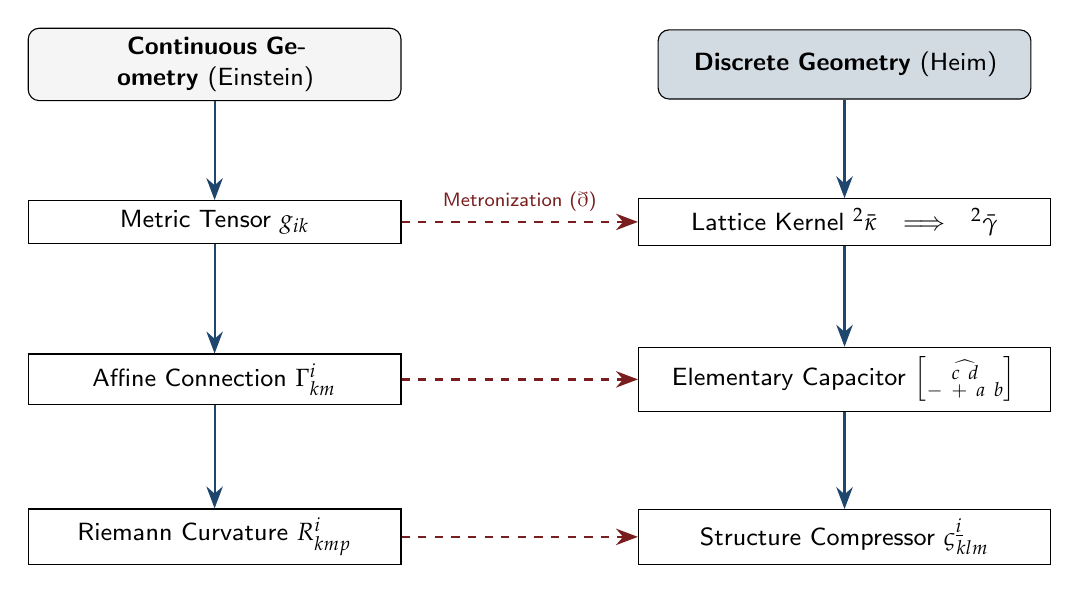
\begin{tikzpicture}[
    node distance=0.6cm,
    process/.style={rectangle, draw, fill=theoryblue!10, rounded corners, minimum height=2.5em, text width=4.5cm, text centered, font=\sffamily\small},
    base/.style={draw, thin, fill=white, align=center, font=\fontsize{9pt}{11pt}\selectfont\sffamily},
    arrow/.style={-{Stealth[scale=1.2]}, thick, theoryblue},
    dashedarrow/.style={-{Stealth[scale=1.2]}, dashed, thick, theoryred}
]

    % Continuous Side
    \node[process, fill=theorygray] (gr) at (-4, 2) {\textbf{Continuous Geometry} (Einstein)};
    \node[base, text width=4.5cm] (metric) at (-4, 0) {Metric Tensor $g_{ik}$};
    \node[base, text width=4.5cm] (christoffel) at (-4, -2) {Affine Connection $\Gamma^i_{km}$};
    \node[base, text width=4.5cm] (riemann) at (-4, -4) {Riemann Curvature $R^i_{kmp}$};

    \draw[arrow] (gr.south) -- (metric.north);
    \draw[arrow] (metric.south) -- (christoffel.north);
    \draw[arrow] (christoffel.south) -- (riemann.north);

    % Discrete Side
    \node[process, fill=theoryblue!20] (heim) at (4, 2) {\textbf{Discrete Geometry} (Heim)};
    \node[base, text width=5cm] (kernel) at (4, 0) {Lattice Kernel ${}^2\bar{\kappa} \implies {}^2\bar{\gamma}$};
    \node[base, text width=5cm] (capacitor) at (4, -2) {Elementary Capacitor $\metroncap{\widehat{c \ d}}{- \ +}{a \ b}$};
    \node[base, text width=5cm] (compressor) at (4, -4) {Structure Compressor $\varsigma^{\underline{i}}_{klm}$};

    \draw[arrow] (heim.south) -- (kernel.north);
    \draw[arrow] (kernel.south) -- (capacitor.north);
    \draw[arrow] (capacitor.south) -- (compressor.north);

    % Mapping Arrows
    \draw[dashedarrow] (metric.east) -- (kernel.west) node[midway, above, font=\scriptsize\sffamily, theoryred] {Metronization ($\ethop$)};
    \draw[dashedarrow] (christoffel.east) -- (capacitor.west);
    \draw[dashedarrow] (riemann.east) -- (compressor.west);

\end{tikzpicture}
\end{adjustbox}
\caption{The translation of continuous General Relativity into Heim's discrete Metron Selector Theory.}
\end{figure}

\subsubsection{The Metron Lattice Equation and Correlation Tensor}
When a particle moves through this discrete space, the continuous geodesic equation ($\ddot{x}^i + \Gamma^i_{kl}\dot{x}^k\dot{x}^l = 0$) translates into the \textbf{Metron Lattice Equation}:
\begin{equation}
    \ethop^2_p n^{\underline{i}} + \frac{\alpha_k \alpha_l}{\alpha_i} \ethop_p n^{\underline{k}} \ethop_p n^{\underline{l}} \metroncap{i}{k\ l}{(c,d) - + (a,b)}; n = 0
\end{equation}

Furthermore, because polymetrics involve overlapping dimensions, Heim introduces the \textbf{Correlation Tensor} ($Q$) to account for correlated metrics. The hyperstructure operator defining the deviation from an uncorrelated state is:
\begin{equation}
    \widehat{[\ ]} = \sum_{\alpha=1}^{\omega^4} \left( \metroncap{\widehat{(c\ d)}}{-\ +}{(a\ b)} + \operatorname{sp} {}^2\bar{Q}(\alpha); () \times \metroncap{\widehat{(c\ d)}}{-\ +}{(a\ b)} \right)
\end{equation}
\section{The World Selector (\texorpdfstring{$L;\widehat{[\ ]} = {}^4\bar{0}$}{L;[] = 0})}

With the continuous Riemann curvature tensor ($R^\mu_{\nu\lambda\kappa}$) successfully replaced by the discrete Structure Compressor ($\varsigma^{\underline{i}}_{klm}$), Heim can finally formulate the ultimate governing equation of his unified theory.

In continuous physics, Einstein equated curvature to the matter tensor ($G_{ik} = \kappa T_{ik}$). Because Heim treats matter as a specific, stable resonance of the geometry itself, he does not set the curvature equal to an external matter source. Instead, he sets up an \textbf{Eigenvalue Problem} for the geometric connections.

Heim defines the \textbf{World Selector} (\textit{Weltselektor}) by the following operator equation:
\begin{equation}
    L;\widehat{[\ ]} = {}^4\bar{0} \quad \text{where } L = K - \bar{\lambda} \times ()
\end{equation}

When applied to the Elementary Capacitor (the discrete connection), this World Selector generates the primary requirement for a stable metronized lattice:
\begin{tcolorbox}[colback=white, colframe=theoryred, title=\textbf{The World Selector Eigenvalue Equation}]
\begin{equation}
    K_m; \metroncap{i}{k\ l}{ } = \underline{\ethop}_l \metroncap{i}{k\ m}{ } - \underline{\ethop}_m \metroncap{i}{k\ l}{ } + \metroncap{i}{l\ s}{ }; () \metroncap{s}{k\ m}{ } - \metroncap{i}{m\ s}{ }; () \metroncap{s}{k\ l}{ } = \lambda_m(k, l) \metroncap{i}{k\ l}{ }
\end{equation}
\end{tcolorbox}
Here, $\underline{\ethop}_l \equiv \frac{1}{\alpha_l}\ethop_l$ represents the normalized metron derivative. 

This equation is profound. It states that the discrete structure compressor acting on the geometry ($\metroncap{i}{k\ l}{ }$) must return the exact same geometry multiplied by a set of eigenvalues $\lambda_m(k, l)$. These eigenvalues are the discrete, quantum-like structural steps of the curvature. 

\textbf{Physical Meaning:} The material world is a set of eigenvalue spectra. An elementary particle (like an electron or proton) exists \textit{only} where this equation holds true—where the geometric flux cycles upon itself and achieves a stable resonant eigenvalue $\lambda$. 

\subsection{Solving the Basic Hermetry Problem}

To solve this massive system of partial difference equations and find the exact geometric shape of these "knots," Heim evaluates the \textbf{Hermetry Forms}—the specific ratios of the eigenvalues that allow for a closed, stable circulatory system.

Heim introduces a dimensionless coupling ratio $a_{ml}$, defined by the components where the indices match ($k=m$):
\begin{equation}
    a_{ml} = -\frac{\lambda_l(m, m)}{\lambda_m(m, l)} \implies \metroncap{i}{m\ l}{ } = a_{ml} \metroncap{i}{m\ m}{ }
\end{equation}
By substituting these ratios back into the World Selector components, Heim reduces the tensorial rank, collapsing the complex system into a manageable metron partial differential equation:
\begin{equation}
    \left( (a(k, l)-1)\underline{\ethop}_l - \sum_{l \neq m} \underline{\ethop}_m \right); \varphi_{kl} + \varphi_{kl}^2 = \lambda(k, l)\varphi_{kl}
\end{equation}

\subsubsection{The Geometric Integration}

To integrate this discrete PDE, Heim transforms the structural problem into a metronic gradient problem:
\begin{equation}
    \bar{a}_{kl} \mathrm{GRAD}_q \varphi_{kl} = \lambda(k,l)\varphi_{kl} - \varphi_{kl}^2
\end{equation}

By introducing the variable $u = \pm (\frac{2\varphi_{kl}}{\lambda(k, l)} - 1)$, the gradient is related directly to the Metron number $\bar{n}$. Multiplying by the metron increment $\ethop \bar{n}$, the right side becomes a constant $\Lambda_{kl}$:
\begin{equation}
    \frac{\ethop u}{1 - u^2} = \pm \frac{1}{2} \lambda(k, l) \ethop N_{kl} = \pm \Lambda_{kl}
\end{equation}

Applying the rules of metron integration (specifically the macroscopic exponential approximation $\ethop \ln \varphi \approx \ethop \varphi / \varphi$ established in Chapter 7), Heim integrates the gradient to find the structural ground state.

\begin{tcolorbox}[colback=white, colframe=theoryblue, title=\textbf{The Fundamental Structural Integral}]
The complete first metron integral of the world structure—the solution that defines the stable existence of localized mass—is written as:
\begin{equation}
    (E - \Psi_{kl})^{\Lambda_{kl} + 1} \cdot \Psi_{kl}^{\Lambda_{kl} - 1} = 2^{-2\Lambda_{kl}} \cdot C_{kl} e^{-\lambda_{kl} \mu}
\end{equation}
Where $\Psi_{kl}$ is the normalized metric connection, and the coefficients are defined by the structural eigenvalues:
\begin{equation}
    \Lambda_{kl} = \alpha_l (a(k, l) - 1)^{-1} - \sum_{m \neq n} \alpha_m, \quad (a(k, l) - q) \cdot \lambda_{kl} = \lambda(k, l)
\end{equation}
\end{tcolorbox}

\textbf{Conclusion of the Marble Building:} 
With this integral, Heim finally completes Einstein's dream of the "Marble Building." The right-hand side of the field equations is no longer "wood" (phenomenological mass $T_{ik}$ added by hand). Instead, localized matter is the exponential solution ($e^{-\lambda_{kl} \mu}$) of the underlying geometry itself. 

Energy cannot be a continuous fluid because the underlying geometric connections ($\Psi_{kl}$) are strictly constrained by the Metron area $\tau$ and the integer eigenvalues $\lambda$. The universe is not a collection of objects moving through an empty container; it is a hyper-dimensional lattice of \textbf{Resonant Selections}. 
% ==============================================================================
% CHAPTER 9: POLYMETRIC WORLD GEOMETRY AND PHYSICAL CLASSIFICATION
% ==============================================================================
% ==============================================================================
\section{Synmetronics and Flux Topology}
\label{sec:synmetronics}
% ==============================================================================
\textit{References: Elementarstrukturen der Materie 2 (Chapters VI \& VII)}

While the World Selector dictates \textit{if} a particle can exist, Heim needed a framework to describe \textit{how} the internal metron fluxes fold and interact to create the specific properties (spin, charge, strangeness) of the particle zoo. He termed this internal polymetry of relative metron condensation \textbf{Synmetronics} (\textit{Synmetronik}).

\subsection{The Straton and the Pseudo-Shield Field}
In Synmetronics, an elementary particle is not a single rotating loop; it is a highly complex aggregate of multiple internal flows. Heim calculates that these internal flux aggregates ($F_v$) are enveloped by a condensation-free pseudo-shield field called the \textbf{Straton}. 

The Straton does not possess discrete mass condensation steps itself, but it dictates the \textit{Ponderability} (the gravitational rest mass) of the complex $c$- and $d$-hermetry forms. Heim defines a specific quantum number for this enveloping field, the \textbf{Stratonspin} ($\sigma_r$):
\begin{equation}
    \overline{s}_x = \sum_{\mu, p, q} \mathbb{P}_x(\mu)^q = \pm \overline{s}_0 \hbar m_x / 2
\end{equation}
This mathematical distinction explains why some particles exhibit spatial Gegenständlichkeit (tangibility/ponderability) while others (like photons) do not, purely based on whether the Stratonspin evaluates to a real or imaginary number depending on the parity of the spatial spin $Q$.

\subsection{Enantiostereoisomerism of Flux Aggregates}
Because these metron fluxes exist in a 6-dimensional space, they exhibit topological properties similar to chiral molecules in organic chemistry. Heim borrows the chemical term \textbf{Enantiostereoisomerism} to describe how these fluxes fold.

For any given stable flux aggregate in $R_6$, there exists a spatially mirror-symmetric (enantiomorphic) arrangement. This provides the strict geometric basis for \textbf{Antimatter}. An antiparticle is simply the enantiostereoisomeric reflection of the metron flux aggregate, where the geometric "clasps" (\textit{Konjunktoren}) binding the flux orient in the opposite $S_2$ direction.

\begin{figure}[htbp]
\centering
\begin{adjustbox}{max width=0.8\textwidth}
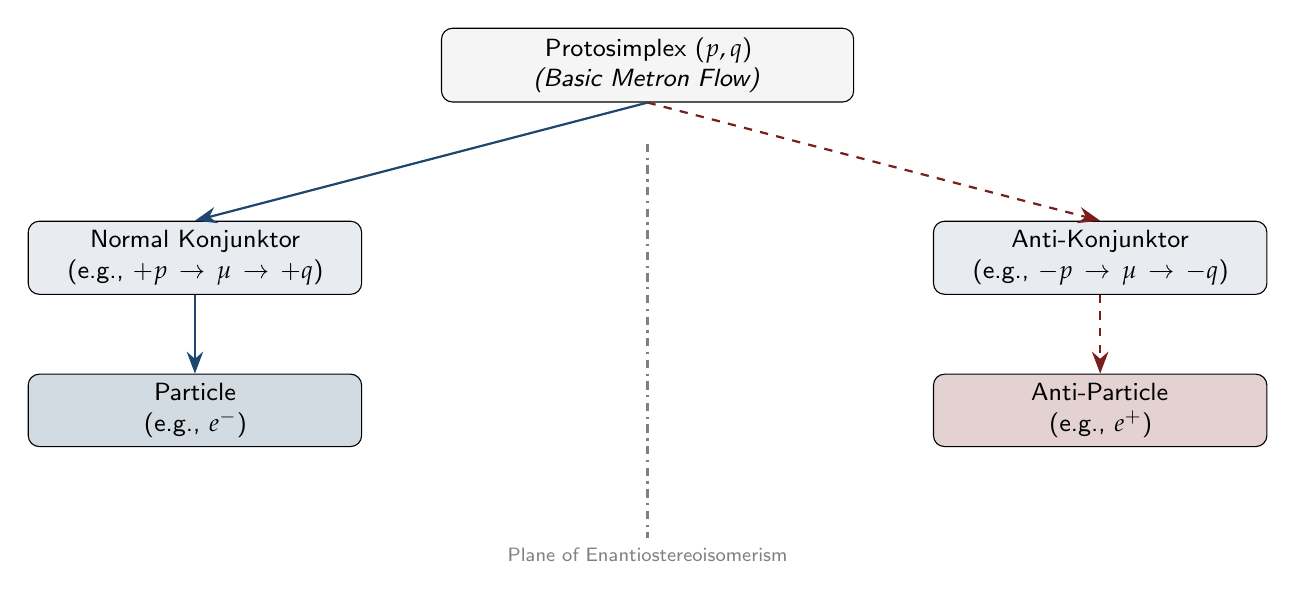
\begin{tikzpicture}[
    node distance=0.6cm,
    process/.style={rectangle, draw, fill=theoryblue!10, rounded corners, minimum height=2.5em, text width=4cm, text centered, font=\sffamily\small},
    arrow/.style={-{Stealth[scale=1.2]}, thick, theoryblue},
    dashedarrow/.style={-{Stealth[scale=1.2]}, dashed, thick, theoryred}
]
    % Central Node
    \node[process, fill=theorygray, text width=5cm] (proto) {Protosimplex ($p, q$)\\ \textit{(Basic Metron Flow)}};

    % Left Branch (Matter)
    \node[process, below left=1.5cm and 1cm of proto] (matter) {Normal Konjunktor\\ (e.g., $+p \to \mu \to +q$)};
    \node[process, below=1cm of matter, fill=theoryblue!20] (part) {Particle\\ (e.g., $e^-$)};

    % Right Branch (Antimatter)
    \node[process, below right=1.5cm and 1cm of proto] (anti) {Anti-Konjunktor\\ (e.g., $-p \to \mu \to -q$)};
    \node[process, below=1cm of anti, fill=theoryred!20] (apart) {Anti-Particle\\ (e.g., $e^+$)};

    \draw[arrow] (proto.south) -- (matter.north);
    \draw[dashedarrow] (proto.south) -- (anti.north);
    \draw[arrow] (matter.south) -- (part.north);
    \draw[dashedarrow] (anti.south) -- (apart.north);

    % Symmetry line
    \draw[thick, dash dot, gray] (0, -1) -- (0, -6) node[below, font=\scriptsize\sffamily] {Plane of Enantiostereoisomerism};

\end{tikzpicture}
\end{adjustbox}
\caption{The topological folding of metron fluxes. Matter and Antimatter are mirror-image geometric configurations (Enantiostereoisomers) of the same underlying Protosimplex.}
\end{figure}

\subsection{The 18 Kopplungsgruppen (Coupling Groups)}
Heim demonstrates that the 72 possible Kondensoren, which define how particles interact across the metron grid, are not random. They organize themselves into exactly 18 \textit{Kopplungsgruppen} (Coupling Groups). 

These groups classify the interactions by their symmetry:
\begin{itemize}
    \item \textbf{Diagonale (d):} 1d, 2d, 3d, 4d, 5d, 6d.
    \item \textbf{Semidiagonale (s):} 1s, 2s, 3s, 4s, 5s, 6s.
    \item \textbf{Extradiagonale (e):} 1e, 2e, 3e.
\end{itemize}

Each group acts as a "logic gate" for the structural condensation. For example, a $d$-type coupling group forces the $R_6$ flux to project into our 3D space as a charged lepton or quark. The 18 groups are not arbitrary; they are the result of the \textbf{Permutations of the Kondensorsignaturen} (Volume 2, Page 147). This proves that the hierarchy of the Standard Model is actually a direct reflection of the geometric symmetry groups of the $R_6$ hyperstructure.

\section{The Concept of Polymetrics}
\label{sec:polymetrics}

\textit{References: MBB Lecture Transcript (Part 9); Map "4 kinds of physical interactions in R6"}

To understand how the 6-dimensional hyperstructure ($R_6$) interacts with our observable universe, Heim moved beyond standard Riemannian geometry into \textbf{Polymetric World Geometry}. 

In standard physics, a single metric tensor ($g_{ik}$) describes the curvature of a space. In the 1940s, physicists like Nathan Rosen attempted to eliminate singularities by introducing "bimetric" gravity (using two interacting metrics). Heim took this concept to its ultimate logical conclusion. Because $R_6$ is composed of three distinct subspaces—$R_3$ (Space), $T$ (Time), and $S_2$ (Structure)—the total geometry must be governed by the interactions of multiple metrics.

Heim defined a non-Hermitian structural unit $\kappa_{ik}^{(\lambda)}$ for each of the three subspaces ($\lambda = 1, 2, 3$):
\begin{itemize}
    \item \textbf{$\lambda = 1$:} Governs the internal, imaginary coordinates $x_5, x_6$ ($S_2$).
    \item \textbf{$\lambda = 2$:} Governs the imaginary time coordinate $x_4$ ($T$).
    \item \textbf{$\lambda = 3$:} Governs the real spatial coordinates $x_1, x_2, x_3$ ($R_3$).
\end{itemize}

When a physical event occurs, these structural units interact multiplicatively. The product of two structural units forms a fundamental tensor $\gamma$:
\begin{equation}
    \gamma_{ik}^{(\mu\nu)} = \sum_{m=1}^6 \kappa_{im}^{(\mu)} \kappa_{mk}^{(\nu)}
\end{equation}
Because these units are non-Hermitian ($\gamma_{ik}^{(\mu\nu)} \neq \gamma_{ki}^{(\mu\nu)}$), their combinations allow for up to nine distinct, interrelated geometries (\textit{Eneametry}).
\subsection{The Structure of the \texorpdfstring{$R_6$}{R6} Metric Tensor}

The polymetric geometry can be represented by the $6 \times 6$ fundamental metric tensor $g_{ik}$. In Heim's framework, this tensor is partitioned into distinct block matrices that govern the observable and hidden dimensions:

\begin{equation}
    g_{ik}^{(6)} = \left(
    \begin{array}{ccc|c|cc}
    g_{11} & g_{12} & g_{13} & g_{14} & \cellcolor{theoryred!10}0 & \cellcolor{theoryred!10}0 \\
    g_{21} & g_{22} & g_{23} & g_{24} & \cellcolor{theoryred!10}0 & \cellcolor{theoryred!10}0 \\
    g_{31} & g_{32} & g_{33} & g_{34} & \cellcolor{theoryred!10}0 & \cellcolor{theoryred!10}0 \\ \hline
    g_{41} & g_{42} & g_{43} & g_{44} & \cellcolor{theoryblue!10}g_{45} & \cellcolor{theoryblue!10}g_{46} \\ \hline
    \cellcolor{theoryred!10}0 & \cellcolor{theoryred!10}0 & \cellcolor{theoryred!10}0 & \cellcolor{theoryblue!10}g_{54} & g_{55} & g_{56} \\
    \cellcolor{theoryred!10}0 & \cellcolor{theoryred!10}0 & \cellcolor{theoryred!10}0 & \cellcolor{theoryblue!10}g_{64} & g_{65} & g_{66} \\
    \end{array}
    \right)
\end{equation}

Here, the upper-left $3 \times 3$ block represents purely spatial coordinates ($R_3$). The cross-terms bounded in red are strictly zero ($g_{s\sigma} = 0$ for $s \in \{1,2,3\}$ and $\sigma \in \{5,6\}$). This is why the organizational dimensions $x_5$ and $x_6$ cannot be perceived directly by human senses or 3D instruments. They only interact with physical space indirectly through the temporal cross-terms ($g_{45}, g_{46}$, bounded in blue).

\section{The Four Hermetry Forms}

Not all nine combinations produce stable physical phenomena. Heim established four primary classes of physical interaction—the \textbf{Hermetry Forms}—based on whether the structural units act as unit tensors (Kronecker deltas, $\delta_{ik}$). If a structural unit equals $\delta_{ik}$, it is essentially "inactive" or "flat" with respect to that specific interaction.

\begin{table}[htbp]
\centering
\renewcommand{\arraystretch}{1.5}
\begin{tabular}{|c|p{3.5cm}|p{2cm}|p{6cm}|}
\hline
\rowcolor{theoryblue!10}
\textbf{Type} & \textbf{Active Coordinates} & \textbf{Subspaces} & \textbf{Physical Interpretation \& Solution} \\ \hline
\textbf{A} & $x_5, x_6$ \newline (Bimetry) & $S_2$ & Operates outside of observable space-time. Influences gravitation (gravitons). Solves for \textbf{Field Masses}. \\ \hline
\textbf{B} & $x_4, x_5, x_6$ \newline (Temporal Hexametry) & $T \cup S_2$ & Entities moving at the speed of light without retardation. The electromagnetic field. Solves for \textbf{Photons}. \\ \hline
\textbf{C} & $x_1, x_2, x_3, x_5, x_6$ \newline (Spatial Hexametry) & $R_3 \cup S_2$ & Ponderable matter that possesses inertia but no net electric field. Solves for \textbf{Neutral Elementary Mass}. \\ \hline
\textbf{D} & $x_1, x_2, x_3, x_4, x_5, x_6$ \newline (Eneametry) & $R_3 \cup T \cup S_2$ & Fully active across all dimensions. Ponderable matter with an electric charge field. Solves for \textbf{Elementary Charge}. \\ \hline
\end{tabular}
\caption{The Four Hermetry Forms defining all physical interactions in $R_6$.}
\end{table}

This classification achieves what the Standard Model must postulate by hand. It proves geometrically why photons possess no rest mass (they lack the $R_3$ spatial component) and why charged particles are the most complex entities in the universe (they require the full enea-metric interaction of all 6 dimensions).

\section{Classification in the System of Known Physical Theories}
\label{sec:classification}

\textit{References: Map "Classification in the system of known physical theories" (Page 6)}

Heim's unified field theory is not a replacement for 20th-century physics; it is the geometric "parent" from which all known continuous theories naturally emerge as specific, limited approximations.

By applying the Matrix Trace to the 6-dimensional World Selector and taking specific mathematical limits, Heim successfully derived the foundational equations of General Relativity, Maxwell's Electrodynamics, and Quantum Mechanics. 

\begin{figure}[htbp]
\centering
\begin{adjustbox}{max width=\textwidth}
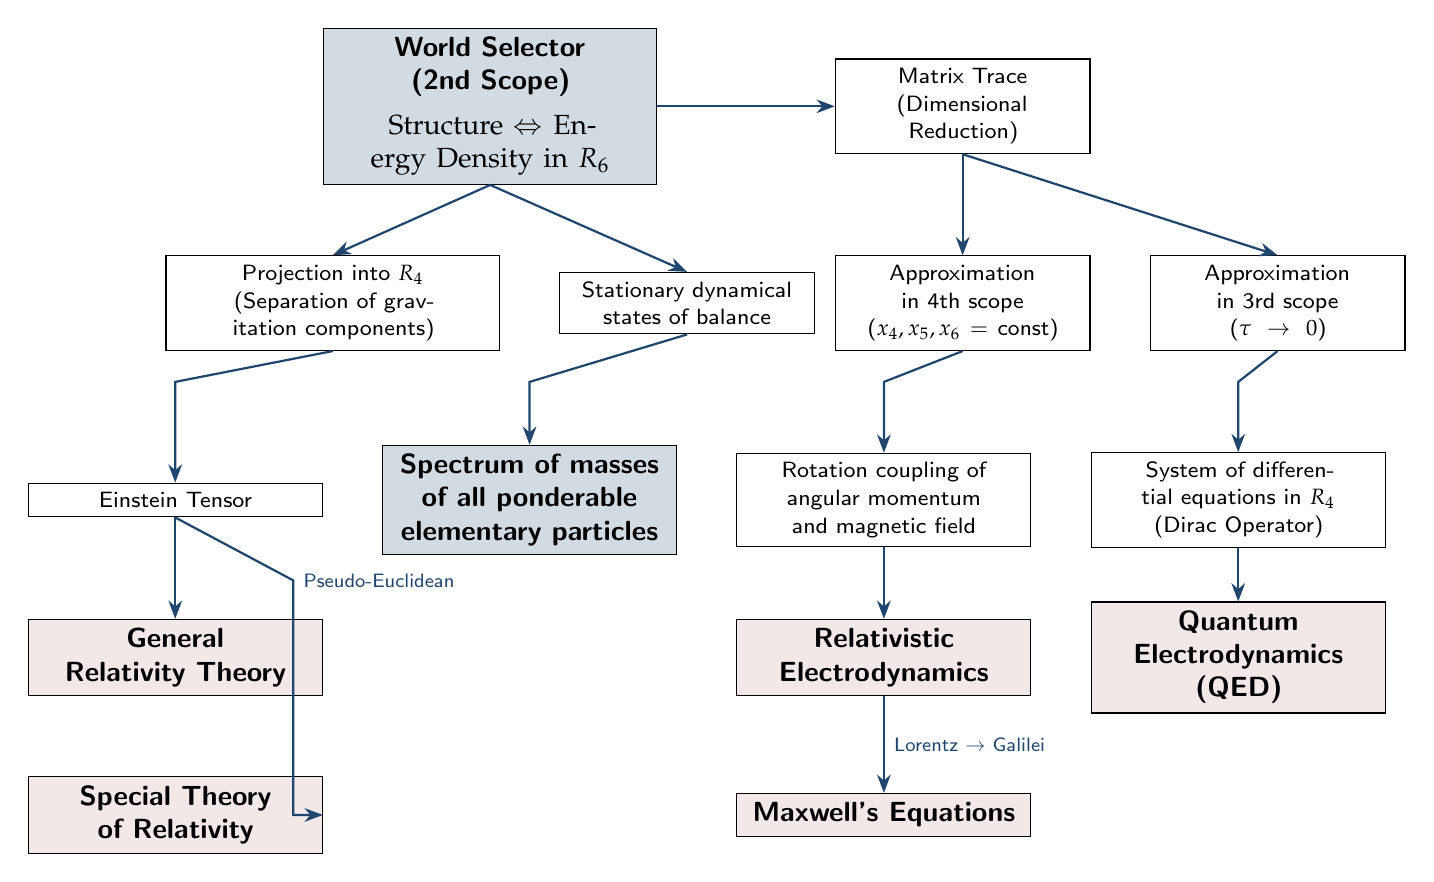
\begin{tikzpicture}[
    node distance=0.5cm,
    base/.style={draw, thin, fill=white, align=center, font=\fontsize{8pt}{10pt}\selectfont\sffamily},
    databox/.style={base, fill=theorygray, font=\bfseries\sffamily},
    arrow/.style={-{Stealth[scale=1.0]}, thick, theoryblue}
]

    % --- TOP LEVEL: HEIM THEORY ---
    \node[databox, text width=4cm, fill=theoryblue!20] (world) at (0, 0) {World Selector\\ (2nd Scope)\\[4pt] \normalfont Structure $\Leftrightarrow$ Energy Density in $R_6$};
    
    \node[base, text width=3cm] (trace) at (6, 0) {Matrix Trace\\ (Dimensional Reduction)};
    \draw[arrow] (world) -- (trace);

    % --- MIDDLE LEVEL: APPROXIMATIONS ---
    \node[base, text width=4cm] (proj) at (-2, -2.5) {Projection into $R_4$\\ (Separation of gravitation components)};
    
    \node[base, text width=3cm] (stat) at (2.5, -2.5) {Stationary dynamical states of balance};
    
    \node[base, text width=3cm] (approx4) at (6, -2.5) {Approximation in 4th scope\\ ($x_4, x_5, x_6 = \text{const}$)};
    
    \node[base, text width=3cm] (approx3) at (10, -2.5) {Approximation in 3rd scope\\ ($\tau \to 0$)};

    \draw[arrow] (world.south) -- (proj.north);
    \draw[arrow] (world.south) -- (stat.north);
    \draw[arrow] (trace.south) -- (approx4.north);
    \draw[arrow] (trace.south) -- (approx3.north);

    % --- BOTTOM LEVEL: KNOWN THEORIES ---
    % General Relativity
    \node[base, text width=3.5cm] (einstein) at (-4, -5) {Einstein Tensor};
    \node[databox, text width=3.5cm, fill=theoryred!10] (gr) at (-4, -7) {General\\ Relativity Theory};
    \node[databox, text width=3.5cm, fill=theoryred!10] (sr) at (-4, -9) {Special Theory\\ of Relativity};
    
    \draw[arrow] (proj.south) -- (-4, -3.5) -- (einstein.north);
    \draw[arrow] (einstein.south) -- (gr.north);
    \draw[arrow] (einstein.south) -- ++(1.5, -0.8) node[right, font=\scriptsize\sffamily] {Pseudo-Euclidean} |- (sr.east);

    % Heim Mass Formula
    \node[databox, text width=3.5cm, fill=theoryblue!20] (mass) at (0.5, -5) {Spectrum of masses of all ponderable elementary particles};
    \draw[arrow] (stat.south) -- (0.5, -3.5) -- (mass.north);

    % Electrodynamics
    \node[base, text width=3.5cm] (rot) at (5, -5) {Rotation coupling of\\ angular momentum\\ and magnetic field};
    \node[databox, text width=3.5cm, fill=theoryred!10] (relelec) at (5, -7) {Relativistic\\ Electrodynamics};
    \node[databox, text width=3.5cm, fill=theoryred!10] (maxwell) at (5, -9) {Maxwell's Equations};
    
    \draw[arrow] (approx4.south) -- (5, -3.5) -- (rot.north);
    \draw[arrow] (rot.south) -- (relelec.north);
    \draw[arrow] (relelec.south) -- node[right, font=\scriptsize\sffamily] {Lorentz $\to$ Galilei} (maxwell.north);

    % Quantum Mechanics
    \node[base, text width=3.5cm] (dirac) at (9.5, -5) {System of differential equations in $R_4$\\ (Dirac Operator)};
    \node[databox, text width=3.5cm, fill=theoryred!10] (qed) at (9.5, -7) {Quantum\\ Electrodynamics (QED)};
    
    \draw[arrow] (approx3.south) -- (9.5, -3.5) -- (dirac.north);
    \draw[arrow] (dirac.south) -- (qed.north);

\end{tikzpicture}
\end{adjustbox}
\caption{The logical reduction of Heim's 6-dimensional World Selector into the established continuous theories of 20th-century physics.}
\end{figure}

\subsection{Deriving the Macrosphere from the Microcosm}

The flowchart above illustrates exactly how Heim bridged the "Double Way":

\begin{enumerate}
    \item \textbf{General Relativity (Gravity):}
    By projecting the World Selector from $R_6$ down into the $R_4$ subspace and mathematically separating the gravitational components, Heim recovers the \textbf{Einstein Tensor}. If the space is assumed to be pseudo-Euclidean (flat), this further reduces to the \textbf{Special Theory of Relativity}.
    
    \item \textbf{Quantum Electrodynamics (QED):}
    If one takes the limit where the Metron area approaches zero ($\tau \to 0$)—effectively treating space as a continuous fluid again—the discrete difference operators ($\ethop$) transform back into infinitesimal differentials ($d$). In this "3rd scope" approximation, the structural equations reduce perfectly to the \textbf{Dirac Operator}, establishing the foundation for Quantum Electrodynamics.
    
    \item \textbf{Maxwell's Equations:}
    If the imaginary organizational dimensions are held constant ($x_4, x_5, x_6 = \text{const}$), the rotational coupling of the angular momentum density yields \textbf{Relativistic Electrodynamics}. Transitioning from the Lorentz group back to the Galilean group recovers the classical \textbf{Maxwell Equations}.
\end{enumerate}

\begin{tcolorbox}[colback=white, colframe=theoryblue, title=\textbf{Conclusion of the Polymetric Architecture}]
Heim's Polymetric World Geometry proves that Quantum Mechanics and General Relativity are not fundamentally incompatible. Their apparent contradictions arise solely because both theories are incomplete, lower-dimensional approximations of a 6-dimensional discrete hyperstructure. 

When the Metron ($\tau$) is acknowledged, and the two extra dimensions ($x_5, x_6$) are included, the infinities of Quantum Mechanics disappear, and the missing quantum principles of General Relativity are fulfilled. The universe is geometrically unified.
\end{tcolorbox}
% ==============================================================================
% CHAPTER 10: THE 12-DIMENSIONAL BACKGROUND AND THE ORIGIN OF LIFE
% ==============================================================================

\section{The Non-Material Background of the World (\texorpdfstring{$R_{12}$}{R12})}
\label{sec:r12_background}

\textit{References: Elementarstrukturen der Materie 3; Map "Classification in the system of known physical theories" (Page 6)}

Up to this point, our mathematical derivations have been restricted to the \textbf{Material World} ($R_6$), which contains the real space ($R_3$), time ($T$), and the imaginary organizational structures ($S_2$) responsible for elementary particles and fields. 

However, Heim realized that the "World Selector" operators governing the $R_6$ flux must themselves be driven by a higher-order logic. If the universe is a projection of geometric probabilities (as demonstrated by the eigenvalue equations), where do those probabilities reside? 

To answer this, Heim applied the \textbf{Dimensional Law for Hyper-spaces} one final time. If the material world $R_6$ is treated as the subspace ($p=6$), then its encompassing hyperspace $n$ is calculated as:
\begin{equation}
    (n-1)^2 - 1 = p(p-1)(p-2) \implies (n-1)^2 - 1 = 6(5)(4) = 120 \implies (n-1)^2 = 121 \implies \mathbf{n = 12}
\end{equation}

The ultimate mathematical container of reality is the \textbf{12-Dimensional Space ($R_{12}$)}. Heim splits this space into two halves: the material world ($R_6$) and the non-material background ($V_6$).

\begin{equation}
    R_{12} = \underbrace{R_3 (\text{Space}) + T (\text{Time}) + S_2 (\text{Structure})}_{R_6 \text{ (Material World)}} + \underbrace{I_2 (\text{Information}) + G_4 (\text{Background})}_{V_6 \text{ (Non-Material Background)}}
\end{equation}

\subsection{The Coordinate Allocation of \texorpdfstring{$R_{12}$}{R12}}

To manage this mathematically, Heim maps the $k$-number index to the coordinates across the five distinct subspaces of the $R_{12}$ continuum:

\begin{table}[htbp]
\centering
\renewcommand{\arraystretch}{1.5}
\begin{tabular}{llll}
\toprule
\textbf{Subspace} & \textbf{Coordinates} & \textbf{$k$-Index} & \textbf{Nature} \\
\midrule
\rowcolor{theoryblue!5}
$\mathbf{R_3}$ (Space) & $x_1, x_2, x_3$ & 3 & Real, spatial extent \\
$\mathbf{T}$ (Time) & $x_4$ & 1 & Imaginary, temporal \\
$\mathbf{S_2}$ (Structure) & $x_5, x_6$ & 2 & Imaginary, organization \\
\rowcolor{theorygray}
$\mathbf{I_2}$ (Information) & $x_7, x_8$ & 2 & Timeless, probability amplitudes \\
\rowcolor{theorygray}
$\mathbf{G_4}$ (Background) & $x_9, x_{10}, x_{11}, x_{12}$ & 4 & Timeless, abstract functions ("God only knows") \\
\bottomrule
\end{tabular}
\end{table}
\subsection{The Physical Meaning of Dimensions \texorpdfstring{$x_5$}{x5} and \texorpdfstring{$x_6$}{x6}}
While $R_3$ defines physical space and $x_4$ defines time, Heim recognized that thermodynamics dictates the universe should tend toward ultimate disorder (entropy). The existence of highly organized structures (from stable atoms to biological life) requires a counter-force. Heim assigned this role to the imaginary coordinates of $S_2$:
\begin{itemize}
    \item \textbf{$x_5$ (Entelechy / Aeonic Dimension):} Represents inverse entropy (Negative Entropy or Information). It evaluates the organizational quality of a structure, allowing for the stable accumulation of complexity over time.
    \item \textbf{$x_6$ (Teleology):} Represents goal-directed actualization. It is the geometric axis along which future probability states are "pulled" into present reality. 
\end{itemize}
In standard physics, a particle's trajectory is determined entirely by past causes (determinism). In Heim Theory, because $x_6$ interacts directly with the timeless background, a particle's physical manifestation is partially "steered" by future stable probability states.

\vspace{1em}
\textbf{The Chain of Effects:} 
$G_4$ is defined mathematically as a space of \textbf{4-dimensional, highly symmetrical, timeless processes}. These timeless processes project first into an intermediate general abstract space of functions ($R_n^*$). Through an $n$-dimensional Fourier series expansion, this abstract space generates the probability amplitudes with superposition and interference found in $I_2$. Because $G_4$ is timeless, it has access to any time segment of the material world. $I_2$ controls the organization in $S_2$, which then "selects" the specific structural deformations that manifest in our observable $R_4$ space-time.

\begin{figure}[htbp]
\centering
\begin{adjustbox}{max width=0.85\textwidth}
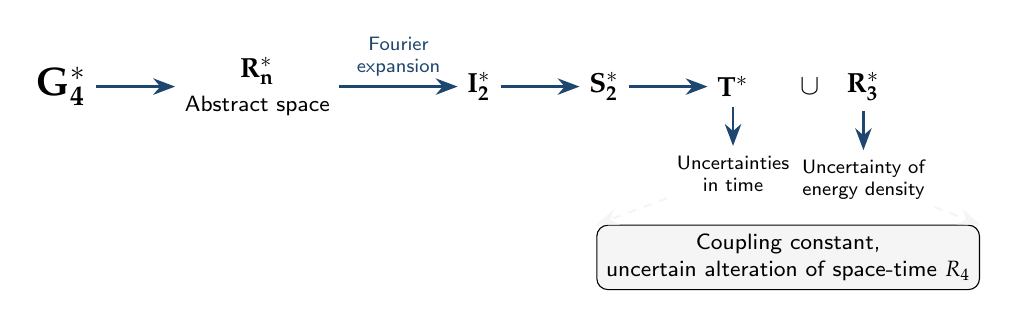
\begin{tikzpicture}[
    node distance=0.5cm,
    arrow/.style={-{Stealth[scale=1.2]}, thick, theoryblue},
    dashedarrow/.style={-{Stealth[scale=1.2]}, dashed, thick, theorygray}
]

    % Main dimensions
    \node[font=\Large\bfseries\sffamily] (g4) {$\mathbf{G_4^*}$};
    \node[font=\normalsize\sffamily, right=1cm of g4, align=center] (rn) {$\mathbf{R_n^*}$\\ \fontsize{8pt}{10pt}\selectfont Abstract space};
    \node[font=\normalsize\sffamily, right=1.5cm of rn, align=center] (i2) {$\mathbf{I_2^*}$};
    \node[font=\normalsize\sffamily, right=1cm of i2] (s2) {$\mathbf{S_2^*}$};
    \node[font=\normalsize\sffamily, right=1cm of s2] (t) {$\mathbf{T^*}$};
    \node[font=\normalsize\sffamily, right=1cm of t] (r3) {$\mathbf{R_3^*}$};
    
    % Connections
    \draw[arrow] (g4) -- (rn);
    \draw[arrow] (rn) -- node[above, font=\scriptsize\sffamily, align=center] {Fourier\\ expansion} (i2);
    \draw[arrow] (i2) -- (s2);
    \draw[arrow] (s2) -- (t);
    \node[right=0.4cm of t] {$\cup$};

    % Uncertainty Mappings
    \node[font=\scriptsize\sffamily, align=center, below=0.5cm of t] (uncT) {Uncertainties\\ in time};
    \node[font=\scriptsize\sffamily, align=center, below=0.5cm of r3] (uncR) {Uncertainty of\\ energy density};
    
    \draw[arrow] (t) -- (uncT);
    \draw[arrow] (r3) -- (uncR);

    % Combination
    \node[draw, thin, rounded corners, fill=theorygray, font=\footnotesize\sffamily, align=center, below=1.5cm of t, xshift=0.7cm] (couple) {Coupling constant,\\ uncertain alteration of space-time $R_4$};
    
    \draw[dashedarrow] (uncT) -- (couple.north west);
    \draw[dashedarrow] (uncR) -- (couple.north east);

\end{tikzpicture}
\end{adjustbox}
\caption{The projection of timeless probability amplitudes from $G_4$ manifesting as Heisenberg uncertainties in $R_4$.}
\end{figure}
\subsection{The Mathematization of Consciousness (The Persona)}
The most controversial, yet mathematically consistent, extension of the $R_{12}$ manifold is Heim's treatment of consciousness. In standard physics, the observer's mind is an unexplained byproduct of chemistry. In Heim Theory, consciousness is a direct, structural necessity of the higher dimensions.

Heim defined the human mind as a highly complex, stable geometric structure operating entirely within the information dimensions $I_2$ ($x_7, x_8$) and the structural dimensions $S_2$ ($x_5, x_6$). He termed this stable 4-dimensional information-structure the \textbf{"Persona"}.

During biological life, the Persona in $I_2 \cup S_2$ projects a Holomorphism (as described in Section 10) down into $R_3$, acting as the organizational clasp that holds the physical brain and body together. The physical brain is merely the hardware interface (the $R_3$ projection) of the mind.

\begin{tcolorbox}[colback=white, colframe=theoryblue, title=\textbf{The Geometric Survival of Information}]
Because the "Persona" structure exists entirely outside of the spatial coordinates ($R_3$) and the temporal coordinate ($T, x_4$), \textbf{it is not subject to thermodynamic entropy}. 

When the physical body dies, the lower-level holomorphisms holding the physical cells together collapse, and the matter in $R_3$ decays. However, the geometric structure of the Persona in $I_2$ remains fully intact. Heim's math implies that consciousness—being a pure information amplitude in the timeless background—cannot be destroyed by physical death. It merely loses its projection into the 3D material space, transitioning fully into the timeless background ($G_4$).
\end{tcolorbox}

\subsection{The Geometric Origin of Quantum Uncertainty}
In the Copenhagen Interpretation of Quantum Mechanics, Heisenberg's Uncertainty Principle ($\Delta x \Delta p \ge \hbar/2$) is assumed to be an inherent, irreducible fuzziness in nature. God, as Einstein complained, appears to play dice.

Heim Theory completely resolves this philosophical crisis. The universe is strictly deterministic, but the determinism occurs in $R_6$, not $R_4$. Because our physical instruments are trapped in the 3D spatial dimensions ($x_1, x_2, x_3$), they can only measure the projection of a 6-dimensional object. 

When the structural coordinates ($x_5, x_6$) of a particle fluctuate, the cross-sections of those fluctuations project down into $R_3$ as probability amplitudes. Thus, \textbf{Quantum Uncertainty is a geometric illusion}. It is the exact mathematical consequence of trying to measure a 6-dimensional rotating metron flux using only a 3-dimensional ruler. The "dice" are not random; they are rolling in dimensions we cannot visually perceive.

\section{Background Independence and the End of the Continuum}

\textit{References: Chat Part 2 — Background Independence and the Metron}

The most significant theoretical achievement of Heim Theory is its strict \textbf{Background Independence}. Modern quantum field theories (and String Theory) are background-dependent; they assume space and time act as a static, continuous stage upon which particles vibrate and interact. 

However, the greatest minds in quantum mechanics suspected that the continuum was a mathematical illusion.
\begin{itemize}
    \item \textbf{Hideki Yukawa} argued: \textit{"The problem of the continuity of time and space is the most difficult... The very existence of elementary particles is connected to the fact that space-time is not a continuum."}
    \item \textbf{Shinichiro Tomonaga} noted that the infinities plaguing quantum field theory—which require the "distorted procedure" of renormalization—arise because \textit{"there are too many degrees of freedom in the space-time continuum."}
\end{itemize}

Heim's introduction of the \textbf{Metron} ($\tau \approx 6.15 \times 10^{-70} \text{ m}^2$) is the exact reduction of degrees of freedom that Tomonaga was searching for. 

\begin{tcolorbox}[colback=white, colframe=theoryblue, title=\textbf{The Resolution of Quantum Infinities}]
By replacing the continuous differential operators ($\diff x$) with the discrete Metron Selector operators ($\ethop$), Heim inherently prevents the formation of singularities. 
\begin{itemize}
    \item A particle cannot collapse into a point of infinite density, because the smallest possible volume is bounded by $\tau$.
    \item Energy cannot climb to infinity, because the spatial frequency spectrum is cut off at the Metron limit.
\end{itemize}
Space is not a container; it is the active, shifting lattice of these finite metron areas. Gravity is simply the localized condensation of this lattice.
\end{tcolorbox}
\section{Empirical Validation and the Mass Formula}

A theory of everything is ultimately judged not by its mathematical elegance, but by its predictive power. Heim's \textbf{World Selector} equation ($L;\widehat{[\ ]} = {}^4\bar{0}$) generated a discrete point spectrum for all ponderable particles without the use of arbitrary fitting parameters or the assumption of a Higgs field.

\subsection{Final Refinement of the Mass Formula}
To account for the high-energy resonances observed in colliders, Heim refined the baseline mass equation to include the resonance-function $F(N)$ and the configurational distributor $\eta$:

\begin{equation}
    M(c,d) = T; m = \mu_+ \left[ \sum_{j=1}^{4} \alpha_j G_j + \left(1 - \frac{\alpha_-}{\alpha_+} \right) F_S + q \frac{\alpha_-}{\alpha_+} \right]
\end{equation}

This formula incorporates the "Sieve Operators" developed in Synmetronics. The term $F_S$ acts as a geometric filter that accounts for the fact that as the quantum number $k$ increases, the metron grid density changes. The mass of a particle is therefore a function of the \textbf{Total Metric Condensation} of its specific configuration, meaning particles are "stable" only at specific geometric resonances of the metron grid.

In 1982, researchers at the Deutsches Elektronen-Synchrotron (DESY) programmed Heim's exact mass formula into a computer. The results provided an unprecedented level of accuracy derived entirely from first geometric principles and fundamental constants ($\gamma, h, \varepsilon_0, \mu_0, c, \pi$).

\begin{table}[htbp]
\centering
\renewcommand{\arraystretch}{1.3}
\begin{tabular}{@{}llcc@{}}
\toprule
\textbf{Particle} & \textbf{Invariant Basic Pattern} & \textbf{Theor. Mass (MeV)} & \textbf{Exp. Mass (MeV)} \\
& $(B, P, Q, \kappa)\varepsilon C(eq_x)$ & \textit{(Heim 1989)} & \textit{(CERN)} \\
\midrule
\rowcolor{theoryblue!5}
Electron ($e^-$) & $e^-: (0,1,1,0)0(-1)$ & 0.5110034 & 0.511 \\
Muon ($\mu^-$) & $\mu^-: (0,1,1,1)0(-1)$ & 105.6595 & 105.658 \\
\rowcolor{theoryblue!5}
Pion ($\pi^\pm$) & $\pi^\pm: (0,2,0,0)0(\pm 1)$ & 139.5670 & 139.570 \\
Kaon ($K^+$) & $K^+: (0,1,0,1)1(+1)$ & 493.6675 & 493.677 \\
\rowcolor{theorygray!20}
Proton ($p$) & $p: (1,1,1,0)0(+1)$ & 938.2797 & 938.272 \\
\rowcolor{theorygray!20}
Neutron ($n$) & $n: (1,1,1,0)0(0)$ & 939.5731 & 939.565 \\
Lambda ($\Lambda$) & $\Lambda: (1,0,1,0)-1(0)$ & 1115.601 & 1115.683 \\
Sigma ($\Sigma^+$) & $\Sigma^+: (1,2,1,0)-1(+1)$ & 1189.357 & 1189.370 \\
Omega ($\Omega^-$) & $\Omega^-: (1,0,3,0)-3(-1)$ & 1672.375 & 1672.450 \\
\bottomrule
\end{tabular}
\caption{Selection from Heim's theoretical mass spectrum (Volume 2, Page 377). The theoretical masses are derived entirely from the invariant basic patterns of the $R_6$ hyperstructure, without using empirical quark masses or the Higgs mechanism.}
\end{table}

\subsection{The Prediction of Neutrino Mass}
Perhaps the greatest historical triumph of Heim Theory lies in its prediction of neutrino mass. Throughout the 20th century, the Standard Model of particle physics assumed that neutrinos were entirely massless, acting exactly like photons. 

However, when Heim evaluated his geometric mass formula for the configuration state $k=1$ and electric charge $q=0$, the World Selector eigenvalue equations refused to yield a zero result. The geometry dictated that these particles must possess a tiny, but non-zero, rest mass.

In 1989, years before experimental physics could test it, Heim published the theoretically derived masses for the free neutrino radiation in $R_3$. In the Appendix of Volume 2 (Page 376), Heim published the following theoretical specific ground states:

\begin{table}[htbp]
\centering
\renewcommand{\arraystretch}{1.3}
\begin{tabular}{ll | ll}
\toprule
\textbf{Neutrino Type} & \textbf{Calculated Mass} & \textbf{Neutrino Type} & \textbf{Calculated Mass} \\
\midrule
\rowcolor{theorygray!20}
$v_R$ (Space-spin)  & $2.003 \text{ eV}$ & $v(e_0)$ (Neutral Electron) & $5.375 \text{ eV}$ \\
$v_p$ (Isoneutrino) & $2.030 \text{ eV}$ & $v_\pi$ (Pion-Neutrino) & $1.441 \text{ KeV}$ \\
\rowcolor{theorygray!20}
$v_\beta$ ($\beta$-Neutrino) & $4.006 \text{ eV}$ & $v_\mu$ (Muon-Neutrino) & $11.287 \text{ KeV}$ \\
\bottomrule
\end{tabular}
\caption{Heim's theoretical predictions for neutrino masses, published nearly a decade before experimental verification of neutrino oscillation.}
\end{table}

It was not until 1998—at the Super-Kamiokande observatory in Japan—that physicists finally detected neutrino oscillation, conclusively proving that neutrinos possess mass, a discovery that won the 2015 Nobel Prize in Physics. Heim had correctly predicted this geometric necessity decades earlier, proving the predictive superiority of the $R_6$ polymetric framework over the Standard Model.

\section{Final Synthesis}

\begin{fancyquote}
    "It is an excerpt from a higher world. To suggest a 'Theory of Everything' or a 'God's Formula' that governs the entire universe might actually indicate a lack of deep reflection." \\
    --- \textit{MBB Lectures (Selector Theory)}
\end{fancyquote}

Burkhard Heim’s framework is arguably the most ambitious geometric unification of physics ever attempted. By demanding that the \textit{Quantum Principle} applies to geometry itself, Heim broke through the 4-dimensional constraints of General Relativity, proving the absolute necessity of a 6-dimensional material hyperspace ($R_6$). 

In doing so, Heim replaced the disjointed zoo of the Standard Model with a singular, elegant truth: \textbf{Matter is condensed geometry.} An electron is not a tiny sphere; it is a 6-dimensional cyclic flux of metronic area-quanta. The Strong Nuclear Force is not a separate field; it is the geometric overlap of external flux zones. Dark Energy is not a mysterious fluid; it is the natural repulsive limit of a field mass acting at galactic distances.

While mainstream physics chose the path of adding continuous fields and background-dependent strings to solve the universe's anomalies, Heim's \textit{Elementarstrukturen der Materie} stands as a towering, highly accurate alternative. It remains a fully realized map of Einstein's Marble Building—waiting for the day when physics is ready to finally abandon the continuum.

\section{Epilogue: Extended Heim Theory (EHT)}
\label{sec:eht}

While Burkhard Heim established the $R_6$ framework to successfully derive the masses of elementary particles, his work did not stop there. In the late 1990s and early 2000s, Walter Dröscher (who provided the mathematical proof of the $R_6$ hyperspace via the improper quotient) and Jochem Hauser expanded Heim's framework into what is now known as \textbf{Extended Heim Theory (EHT)}.

To align Heim's geometric structures with the symmetry groups of the Standard Model of particle physics, Dröscher expanded the $R_6$ metric tensor into an 8-dimensional space ($R_8$). This theoretical leap suggested that the imaginary organizational dimensions could be sub-divided further.

The most profound prediction of EHT is the existence of new fundamental forces that interact directly with gravity. Specifically, the theory posits the existence of \textbf{Gravitophotons}—particles that mediate a repulsive, anti-gravitational force under specific electromagnetic conditions. In 2004, this led to theoretical proposals that a rotating superconducting ring in a strong magnetic field could generate a measurable gravitomagnetic thrust, offering a purely geometric mechanism for propellantless space propulsion. Though currently remaining at the theoretical edge of aerospace engineering, Extended Heim Theory proves that Heim's discrete geometry is a living framework capable of inspiring the next leap in physics.

\hr

\begin{center}
    \textbf{End of Thesis Expansion} \\
    \textit{Based on the MBB Lectures, Metron Calculations, and the structural maps of Olaf Posdzech.}
\end{center}
To align Heim's geometric structures with the Standard Model of particle physics, Dröscher expanded the $R_6$ metric tensor into an 8-dimensional space ($R_8$). By applying group theory to the $8 \times 8$ polymetric tensor, EHT successfully derives the exact symmetry groups of the Standard Model ($U(1) \times SU(2) \times SU(3)$) purely from geometry.

More profoundly, the $R_8$ expansion breaks the metric into \textbf{Six Fundamental Forces}. In addition to the known four (Electromagnetism, Gravity, Strong, and Weak nuclear forces), EHT predicts two new gravity-like interactions originating from the information dimensions ($x_7, x_8$):
\begin{enumerate}
    \item \textbf{Quintessence (Gravito-Electromagnetism):} A repulsive anti-gravitational force mediated by a predicted particle called the \textit{Gravitophoton}.
    \item \textbf{Gravito-Weak Force:} A field that couples gravity directly to the probability amplitudes of the weak nuclear force.
\end{enumerate}

In 2004, the American Institute of Aeronautics and Astronautics (AIAA) awarded a prize to a paper by Hauser and Dröscher detailing how these new forces could be engineered. They proposed that a rapidly rotating superconducting ring exposed to a massive magnetic field could artificially stimulate the generation of Gravitophotons. This would create a localized repulsive gravitational field—offering a purely geometric mechanism for propellantless faster-than-light (FTL) space propulsion. 

\subsection{The "Shadow Mass" and the Bridge to $R_8$}
The mathematical justification for expanding Heim's 6-dimensional framework into 8 dimensions was actually seeded by Heim himself in Volume 1. When analyzing the generation of matter, Heim found that the energy density tensor in $R_6$ becomes non-Hermitian, requiring the introduction of an imaginary mass component.

Heim defined this as the \textbf{Schattenmasse} (Shadow Mass), which accompanies every elementary mass $m_0$:
\begin{equation}
    \overline{m}_0 = \pm m_0 \sqrt{\pm i}
\end{equation}

When this shadow mass is introduced additively into the energy densities, the number of non-vanishing tensor components doubles from 24 to 48. Heim noted that these 48 components can perfectly fit into a tensor schema of \textbf{Rank 8} (an $8 \times 8$ matrix containing 16 vanishing components). 

Walter Dröscher utilized this exact mathematical phenomenon—the necessity of the 8-rank tensor to hold the shadow mass symmetries—to formalize \textbf{Extended Heim Theory (EHT)}. By expanding the metric to $R_8$, EHT successfully derives the exact symmetry groups of the Standard Model ($U(1) \times SU(2) \times SU(3)$) purely from geometry, and predicts the existence of the anti-gravitational \textit{Gravitophoton}.

Though currently resting at the bleeding edge of theoretical physics, Extended Heim Theory proves that Heim's discrete geometry is not a dead historical artifact. It is a living, mathematically rigorous framework capable of inspiring the next great leap in human engineering.

\section{Chat Part 2: Background Independence and the Metron}
% ==============================================================================

Let's start with a conversation between some students in a certain era, on a moonlit night that reflects both good and bad:

\begin{fancyquote}
    ``Hey, why don't we just make space-time into a lattice point?''\\
    The lightning-fast reply was: ``No, that wouldn't maintain rotational symmetry!''\\
    ``I see.'' (Sorry, it's not that simple.)
\end{fancyquote}

This time, I'll mix together various statements made by various professors on this subject. What will we see?

\subsection{The Perspective of the Greats}

\begin{description}
    \item[Mr. R (Carlo Rovelli):] The gravitational field does not extend \textit{into} space, but \textit{is} space itself. This is the concept of General Relativity. It is \textbf{background independent} rather than background dependent. Space is not a container; it is a physical entity.

    \item[Mr. E (Albert Einstein):] Absolute time and potential energy play crucial roles in the Schrödinger equation, but relativity recognizes that these two concepts are fundamentally unacceptable. To escape these difficulties, we must build a theory based on fields and field laws instead of interaction forces.

    Regarding the assumption of the space-time continuum: it has been pointed out that its introduction may be contrary to nature, considering the molecular structure of phenomena in the microscopic world. If we follow Heisenberg’s purely algebraic method, we must, in principle, also \textbf{abandon the space-time continuum}. At present, such an attempt is like trying to breathe in a vacuum.

    \item[Mr. Y (Hideki Yukawa):] The problem of the continuity of time and space is the most difficult, and perhaps the last, problem. The very existence of elementary particles is connected to the fact that space-time is \textbf{not a continuum}. If we extract a point in space-time, surely there is no such thing as a field there?

    \item[Mr. T (Shinichiro Tomonaga):] I think the infinity in quantum field theory comes from the fact that there are too many degrees of freedom in the space-time continuum. Renormalization is a complex and distorted procedure. Perhaps we need to reduce the degrees of freedom in this space. This reduction is what causes the large number of elementary particles to appear.
\end{description}

\subsection{Mr. H (Burkhard Heim) and the Metron}

Heim's explanation bridges these concerns. He argues that energy density is proportional to space-time action density. However, because action is an integer multiple of $h$, a restriction to differential quotients (calculus) is impossible due to divergence. Therefore, a \textbf{geometric final unit} is needed to determine the space-time structure.

The final unit in Heim’s theory is the \textbf{Metron} ($\tau$), a two-dimensional constant of area.

\begin{equation}
    \tau \omega c^2 = \pi \gamma \hbar \tag{Metron Formula}
\end{equation}
Where:
\begin{itemize}
    \item $\tau$: Smallest geometric unit (area).
    \item $\omega$: Gravity propagation speed.
    \item $\gamma$: Universal gravitational constant ($G$).
\end{itemize}

Interestingly, this connects to the uncertainty principle:
\begin{equation}
    \Delta x \Delta p \geq \frac{\hbar}{2} = \frac{\omega c^2}{2 \pi \gamma} \tau
\end{equation}

\hr

\begin{reflectionbox}[title={Notes and Reflections: Inverting Intuition}]
It’s a tough road. Our mathematical intuition is based on 0-dimensional points. To assume that \textbf{Area} comes first (a set of two-dimensional minimum unit areas) and then builds the illusion of a space-time continuum (the ``pseudo-continuum'') requires a complete reversal of thinking.

Heim calls the Planck scale ``speculative'' because he derives the Metron from a deeper geometric necessity in $R_6$. This leads us to the most difficult part of his \textit{Fundamental Structures} (Chapter III), which involves:
\begin{enumerate}
    \item Metrological elemental operations.
    \item Selective structures of primitive structural tension.
    \item Polymetric relative metropolitan concentration.
\end{enumerate}

Are we really going to do that?

\begin{fancyquote}
    ``Hey, about space-time... apparently we just need to make the smallest unit two-dimensional?''\\
    ``Two dimensions? What about rotational symmetry?''\\
    ``Rotational symmetry: conditionally okay. Count back the seconds!''
\end{fancyquote}
\end{reflectionbox}

\begin{sectionrefs}
    \item \href{https://en.wikipedia.org/wiki/The_Order_of_Time}{The Order of Time} by Carlo Rovelli: Source for the "background independence" analogy.
    \item \href{https://en.wikipedia.org/wiki/Hideki_Yukawa}{Hideki Yukawa}: Context for the "Elementary Domains" and questioning the spacetime continuum.
    \item \href{https://en.wikipedia.org/wiki/Shin%E2%80%99ichir%C5%8D_Tomonaga}{Shin'ichirō Tomonaga}: Context for renormalization and the degrees of freedom in the continuum.
    \item \href{https://en.wikipedia.org/wiki/Euclid's_Elements}{Euclid's Elements}: Context for the fundamental definitions of points and surfaces.
\end{sectionrefs}

\hr

\subsection*{In-Depth: The Quantization of Structure (Map I-4)}
\addcontentsline{toc}{subsection}{In-Depth: The Quantization of Structure}

Heim formally resolves the "Wood vs. Marble" dilemma by introducing the Quantum Principle directly into the geometric tensor.

\subsubsection*{1. Energy as Action Density}
Heim redefines the components of the energy density tensor $T_{ik}$. Energy is not just a scalar quantity but the rate of change of Action ($W$) over time.
\begin{equation}
    T_{ik} \sim \frac{dW_{ik}}{d\Omega}
\end{equation}
where $d\Omega$ is the differential element of space-time volume.

\subsubsection*{2. The Quantization of Action}
Empirically, Action is quantized in integer steps of Planck's constant $h$. Heim generalizes this to a complex action tensor:
\begin{equation}
    W_{ik} = h(N_{ik} + iK_{ik}), \quad N, K \in \mathbb{Z}
\end{equation}
Because $N$ and $K$ are integers, the differential $dW$ is mathematically invalid (one cannot differentiate a step function). It must be replaced by the difference $\Delta W$.

\subsubsection*{3. The Density of Action Quanta ($\eta_{ik}$)}
Substituting the difference for the differential, the continuous energy density is replaced by a discrete density of action quanta:
\begin{equation}
    \eta_{ik} = \frac{\Delta N_{ik}}{\Delta \Omega}
\end{equation}
This leads to the final form of the Heim Field Equation:
\begin{equation}
    R_{ik} \sim w \cdot \eta_{ik}
\end{equation}
where $w = \sqrt{-g}$ is the metric weight. This equation states that **Curvature ($R_{ik}$) is directly proportional to the density of Action Quanta ($\eta_{ik}$)**. Space-time curvature is not smooth; it is pixelated by the quanta of action. 
% ==============================================================================
% ==============================================================================
\clearpage
\part{The Mathematics of Discrete Space (Metron Calculus)}

\section{Metron Calculation Part 0: Beyond the Continuum}
% ==============================================================================
\textit{Fundamental Structure, Volume 1, Chapter 3, Part 1}

--- This is the ``end.'' The ``world'' ends here. Or rather, the background-dependent continuum ends here, and we must make a pinhole to see what lies beyond.

\subsection{The Quantization of Area}

In standard calculus, the definite integral of a continuous function $y = f(x) \geq 0$ represents the area under the curve in the interval $a \leq x \leq b$. According to Burkhard Heim, because of the existence of Planck's constant, the geometry of the universe is such that this area must be an \textbf{integer multiple} of a smallest unit, the Metron $\tau$.

In the microscopic world, points and lines are not fundamental. Instead, we must divide the definite integral into multiple intervals such that each sub-area is exactly $\tau$. If we divide the area into $n$ intervals:

\begin{equation}
    \int_{x_0}^{x_n} f(x)dx = n\tau \tag{Metron Quantization}
\end{equation}

% --- DIAGRAM REPLACEMENT FOR metrondivide.png ---
\begin{center}
    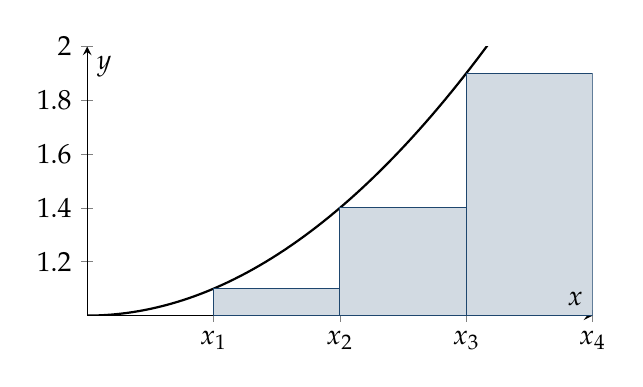
\begin{tikzpicture}
        \begin{axis}[
            axis lines = middle,
            xlabel = $x$,
            ylabel = $y$,
            xtick = {1, 2, 3, 4},
            xticklabels = {$x_1$, $x_2$, $x_3$, $x_4$},
            ymax = 2,
            width = 8cm, height = 5cm
        ]
        \addplot [domain=0:5, samples=100, thick] {1 + 0.1*x^2};
        \addplot [ybar interval, fill=theoryblue!20, draw=theoryblue] coordinates {(1,1.1) (2,1.4) (3,1.9) (4,2)};
        \node at (axis cs: 1.5, 0.5) {$\tau$};
        \node at (axis cs: 2.5, 0.7) {$\tau$};
        \node at (axis cs: 3.5, 0.9) {$\tau$};
        \end{axis}
    \end{tikzpicture}
    \captionof{figure}{Discrete metronization of an integral area.}
\end{center}

In this interpretation, the continuous function $y = f(x)$ is replaced by a sequence of integers $n$ with the dimension of area. The variables become discrete:
\begin{equation}
    x_n = x(n), \quad y_n = f(x_n) = f(n)
\end{equation}

\hr

\begin{reflectionbox}[title={Notes and Reflections: From 4D Lines to 6D Planes}]
``Hey wait, is that all? Isn't it just dividing a definite integral into equal areas?''\\
``Yes. But the implications are massive. A continuous number line doesn't exist in the microscopic world because it is a sequence of unit areas multiplied by integers.''

How many sequences of integers are needed to correspond to a point in the four-dimensional space-time continuum ($x, y, z, t$) at the macro level? In Heim's theory, we don't look at the line elements; we look at the \textbf{planes} formed by choosing two coordinates from four:
\begin{equation}
    n = \binom{4}{2} = \frac{4 \times 3}{2 \times 1} = 6
\end{equation}

The possible planes are: $(x,y), (y,z), (z,x), (x,t), (y,t), (z,t)$.

This is brilliant! We aren't just adding extra dimensions as if they were more lines in a 1D-based space. We are considering a \textbf{six-dimensional integer coordinate system} that corresponds to the six finite surface elements of a 4D spacetime. This is the bridge between the 4D infinitesimal line element of General Relativity and the 6D finite surface elements of Heim Theory.
\end{reflectionbox}

\subsection{A Teaser for Metronic Differentiation}

Next time, we will move away from mundane calculus and introduce \textbf{Metronic Differentiation}. In this discrete world, the standard derivative $dy/dx$ is replaced by a new operator: $\eth$ (the Icelandic letter \textit{eth}).

As we move beyond the ``end'' of the continuum, we find that these operations are what eventually lead to the mass formula for elementary particles.

\begin{sectionrefs}
    \item Burkhard Heim, \textit{Elementary Structure of Matter}, Chapter 3: Fundamental Metron Operations.
    \item Junko Sasaki, \textit{Bremen 5} (1981): Exploring the "end" of space and the utility of $\tau$.
    \item \href{https://en.wikipedia.org/wiki/Definite_integral}{Definite Integral}: Context for the metronization of area ($\tau$).
    \item \href{https://en.wikipedia.org/wiki/Binomial_coefficient}{Binomial Coefficient $\binom{4}{2}$}: Used to derive the six planes of the $R_6$ structure from $R_4$.
    \item \href{https://en.wikipedia.org/wiki/Causal_dynamical_triangulation}{Causal Dynamical Triangulation}: Context for modern research into discrete spacetime geometry.
\end{sectionrefs}

\hr

\subsection*{In-Depth: The Mapping of the Manifolds (Map III-1)}
\addcontentsline{toc}{subsection}{In-Depth: The Mapping of the Manifolds}

To formalize the "pinhole" transition, Heim defines the relationship between the macroscopic coordinates $x_i$ and the microscopic metron digits $n_i$. This is the rigorous proof of the $R_4 \to R_6$ transition.

\subsubsection*{1. The Discrete Coordinate Projection}
In a smooth $R_4$ continuum, a distance is defined by the line element $ds^2$. In a metronized world, this distance is an emergent property of the number of unit surfaces ($\tau$) crossed. Heim introduces the coordinate metronization:
\begin{equation}
    x_i(n) = \alpha_i \cdot n_i \cdot \sqrt{\tau}
\end{equation}
where $\alpha_i$ is a scaling constant. The index $n_i$ must be an integer, reflecting the count of fundamental areas.

\subsubsection*{2. Surface Elements as Basis}
Heim argues that if space is quantized, the fundamental building block cannot be a 1D length, but must be the 2D surface element. In 4 dimensions, the number of independent 2D surfaces (planes) is:
\begin{equation}
    L = \binom{N}{p} = \binom{4}{2} = 6
\end{equation}
This derivation provides the geometric justification for the **6-dimensional manifold** used in the mass calculations. The $R_6$ manifold is not an "extra-dimensional" playground, but the natural space of the surface-quanta of an underlying $R_4$ geometry.

\begin{mbbcite}
    \textbf{Definition of the Metronic Grid:} The world is a hyperstructure where every point in the macroscopic $R_4$ is represented as a complex of 6 integer arguments $(n_1, n_2, n_3, n_4, n_5, n_6)$ in $R_6$. These arguments determine the local metric "condensation" or density of space-time.
\end{mbbcite}

\subsubsection*{3. The Limit of the Pseudo-Continuum}
In the limit where the number of metrons $n$ approach infinity, the discrete structure approximates the Riemannian manifold of Einstein:
\begin{equation}
    \lim_{n \to \infty} \sum_{i} \Delta x_i \approx \int dx
\end{equation}
However, Heim maintains that this limit is never reached in physical reality. The "weirdness" the student felt in the prologue exists because standard physics performs this limit prematurely, losing the information contained in the discrete geometric "twist" of the metrons. 
% ==============================================================================
% ==============================================================================
\section{Metron Calculations Part 1: Basic Operations}
% ==============================================================================
\textit{Metron basic calculation memo 1/3}

The sun's dip angle is 7 degrees, 21 minutes, 40 seconds. The Shogunate Astronomical Observatory announces the time of 6 a.m. (The bell rings.) \textit{Boom... boom...}

\subsection{The Dream Message}

The smallest geometric unit in the universe is two-dimensional, with area $\tau$? That sounds interesting. If we consider circular coordinates, we can even introduce torsion (phase angle). This can connect the end point and the start point in 1/2 rotation units, forming a \textbf{Möbius strip}, allowing us to describe spinors. A simple loop doesn't work this way.

Non-Hermitian connection: a vector shifts the origin by moving it around in a parallel circle. Since all that exists at the beginning is area, there is no secondary background spacetime like points or lines. Spacetime appears through the interrelationships of metrons (\textbf{Background Independence}).

Because it's two-dimensional, even if $\tau$ is constant, the ratio of two metrics can be introduced. This can be interpreted as an amplitude. If spacetime itself can have amplitude and phase, that is reassuring. Note: if we metronize an $n$-dimensional continuum into an $m$-dimensional integer space, the two-dimensionality coincides only when $n=4, m=6$ due to the relationship $\binom{n}{2} = m$. This may be how space perceived as three-dimensional is fundamentally linked to a higher structure.

\subsection{1. Metron Differentiation}

Standard differentiation $f(x)$ is defined as the limit of the difference quotient:
\begin{equation*}
    \frac{df(x)}{dx} = \lim_{\Delta x \to 0} \frac{f(x+\Delta x) - f(x)}{\Delta x}
\end{equation*}

Heim introduces an analogy for the metronic function $\varphi(n)$, where $0 \le n \le N$ and the variable $n$ is an integer. Instead of the differential symbol $d$, we use the Icelandic letter \textbf{eth} ($\eth$). When $\eth$ appears, the variable is an integer sequence of metronic numbers.

The difference quotient of $\varphi(n)$ is:
\begin{equation*}
    \frac{\Delta \varphi}{\Delta n} = \frac{1}{\nu}(\varphi(n) - \varphi(n-\nu))
\end{equation*}

Since $\nu$ is an integer, we cannot take the limit $\nu \to 0$. The minimum possible value is $\nu = +1$. Thus, the metron derivative is defined as:
\begin{equation*}
    \frac{\eth \varphi}{\eth n} = \lim_{\nu \to +1} \frac{1}{\nu}(\varphi(n) - \varphi(n-\nu)) = \varphi(n) - \varphi(n-1)
\end{equation*}

Since $\eth n = 1$, we always have:
\begin{equation}
    \eth \varphi(n) = \varphi(n) - \varphi(n-1), \quad (1 \le n \le N)
\end{equation}

Metron differentiation narrows the domain by one with each operation: $\varphi(n)$ for $(0 \le n \le N)$, $\eth \varphi(n)$ for $(1 \le n \le N)$, $\eth^2 \varphi(n)$ for $(2 \le n \le N)$, and so on.

\subsection{2. Metron Integration}

The inverse operation is metron integration, taking the sum over the metron number. We use $S$ instead of the integral symbol $\int$, where $S \widehat{=} \sum$. If there exists a $\phi$ such that $\varphi = \eth \phi$, then:
\begin{equation*}
    S_{n_1}^{n_2} \varphi \, \eth n = S_{n_1}^{n_2} \eth \phi = \sum_{n=n_1}^{n_2} (\phi(n) - \phi(n-1)) = \phi(n_2) - \phi(n_1-1)
\end{equation*}
\begin{equation}
    J(n_1, n_2) = S_{n_1}^{n_2} \varphi(n) \, \eth n, \quad n_1 \ge 1, n_2 > n_1 \tag{M2a}
\end{equation}

\subsection{3. Higher-order Metron Differential}

Repeating the operation yields:
\begin{align*}
    \eth^0 \varphi &= \varphi \\
    \eth^1 \varphi &= \varphi(n) - \varphi(n-1) \\
    \eth^2 \varphi &= \varphi(n) - 2\varphi(n-1) + \varphi(n-2) \\
    \eth^3 \varphi &= \varphi(n) - 3\varphi(n-1) + 3\varphi(n-2) - \varphi(n-3)
\end{align*}

The general formula follows binomial coefficients:
\begin{equation}
    \eth^k \varphi = \sum_{\nu=0}^{k} (-1)^\nu a_\nu(k) \varphi(n-\nu), \quad a_\nu(k) = \binom{k}{\nu}, \quad 0 \le k \le N \tag{M3}
\end{equation}

\subsection{4. Linearity}
Let $u(n)$ and $v(n)$ be metron functions. For $\varphi = \sum_j u_j(n)$:
\begin{equation}
    \eth \sum_j u_j(n) = \sum_j \eth u_j
\end{equation}

\subsection{5. Constant Rule}
If $\varphi = C$ (constant), then $\varphi = \varphi'$:
\begin{equation}
    \eth C = 0
\end{equation}

\subsection{6. Constant Multiple}
\begin{equation}
    \eth (Cu) = C \eth u
\end{equation}

\subsection{7. Product Rule}
Let $\varphi = uv$. Since $u' = u - \eth u$ and $v' = v - \eth v$:
\begin{equation*}
    \eth(uv) = uv - u'v' = uv - (u - \eth u)(v - \eth v)
\end{equation*}
\begin{equation}
    \eth (uv) = u \eth v + v \eth u - \eth u \eth v
\end{equation}

\subsection{8. Quotient Rule}
For $\varphi = \frac{u}{v}$:
\begin{equation*}
    \eth \left( \frac{u}{v} \right) = \frac{u}{v} - \frac{u'}{v'} = \frac{1}{vv'}(uv' - vu') = \frac{1}{vv'} \begin{vmatrix} u & u' \\ v & v' \end{vmatrix}
\end{equation*}
Using $u' = u - \eth u$ and $v' = v - \eth v$:
\begin{equation*}
    \eth \left( \frac{u}{v} \right) = \frac{1}{vv'} (v \eth u - u \eth v) = \frac{1}{vv'} \begin{vmatrix} \eth u & \eth v \\ u & v \end{vmatrix}
\end{equation*}
where $vv' = v(v - \eth v) = \begin{vmatrix} v & \eth v \\ v & v \end{vmatrix} = v \begin{vmatrix} v & \eth v \\ 1 & 1 \end{vmatrix}$. Thus:
\begin{equation}
    \eth \left( \frac{u}{v} \right) = \frac{1}{v} \begin{vmatrix} \eth u & \eth v \\ u & v \end{vmatrix} \cdot \begin{vmatrix} v & \eth v \\ 1 & 1 \end{vmatrix}^{-1}
\end{equation}

\hr

\textbf{References: \textit{Elementarstrukturen der Materie 1}}
Chapter III: Metron Structure Tensor
\begin{enumerate}
    \item Metron Basic Operations (Summarized above)
    \item Selector
    \item Selector theory of primitive structure tensors
    \item Metron hyperstructure and metronization process
    \item Polymetry of relative metron concentration
\end{enumerate}

\begin{sectionrefs}
    \item \href{https://en.wikipedia.org/wiki/M%C3%B6bius_strip}{Möbius Strip}: Analogy for describing spinors and the phase angle (torsion) in metron geometry.
    \item \href{https://en.wikipedia.org/wiki/Difference_operator}{Difference Operator}: The mathematical concept behind Heim's Metron derivative $\eth$.
    \item \href{https://en.wikipedia.org/wiki/Christoffel_symbols}{Christoffel Symbols}: Context for the non-Hermitian connection in discrete space.
\end{sectionrefs}

\hr

\subsection*{In-Depth: The Formalism of Metron Selectors (Map III-1)}
\addcontentsline{toc}{subsection}{In-Depth: The Formalism of Metron Selectors}

The rules of metron differentiation and integration are more than just discrete analogues to calculus; they are the foundation of **Selector Theory**. In Heim's discrete geometry, an operation is a "Selection" from a range of discrete geometric states.

\subsubsection*{1. The Operator Definition}
Heim formalizes the metron derivative as an operator $C$, called a **Function Selector**. When $C$ acts on a metron function $\varphi$ of argument $n$, it selects the difference between the current state and the previous state:
\begin{equation}
    C; \varphi(n) = \eth \varphi(n) = \varphi(n) - \varphi(n-1)
\end{equation}
The symbol ``;'' is used to denote the application of a selector. Unlike standard calculus, the selector $C$ carries a specific geometric weight related to the Metron area $\tau$.

\subsubsection*{2. Binomial Structure of Higher Orders}
The higher-order metron differential (Eq. M3) reveals that the internal structure of a discrete field is governed by binomial coefficients. For any order $k$:
\begin{equation}
    \eth^k \varphi(n) = \sum_{\nu=0}^{k} (-1)^\nu \binom{k}{\nu} \varphi(n-\nu)
\end{equation}
This suggests that the "curvature" of a metronized field is essentially a weighted sum of its neighboring discrete cells. The stability of a material "knot" (elementary particle) depends on these sums reaching a state of balance ($C; \varphi = 0$).

\subsubsection*{3. The Projective Nature of $\eth$}
Every metron differentiation $\eth$ reduces the available information domain of the function. If $\varphi$ is defined on the range $[0, N]$, then $\eth \varphi$ is defined only on $[1, N]$. This **Projective Property** is what allows Heim to derive lower-dimensional "shadows" (like our 4D space-time) from higher-dimensional 6D structures. The discrete nature ensures that information is never "lost" in a continuum, but merely restricted to specific metron boundaries. 
% ==============================================================================
% ==============================================================================
\section{Metron Calculations Part 2: Advanced Operations}
% ==============================================================================
\textit{Metron basic operation memo 2/3}

\subsection{9. Maximum and Minimum}

As with normal differential calculus, a metron function $\varphi(n)$ has a \textbf{maximum} value for $n$ such that $\eth \varphi = 0$ and $\eth^2 \varphi < 0$. Conversely, $\varphi(n)$ has a \textbf{minimum} value for $n$ such that $\eth \varphi = 0$ and $\eth^2 \varphi > 0$.

\subsection{10. Dividing and Combining Integration Intervals}

When there is an intermediate value $\nu$ between integration intervals $n_1$ and $n_2 \neq n_1$:
\begin{align*}
    S_{n_1}^{n_2} \varphi \, \eth n &= S_{n_1}^{\nu} \varphi \, \eth n + S_{\nu + 1}^{n_2} \varphi \, \eth n \\
    S_{n_1}^{\nu} \varphi \, \eth n + S_{\nu + 1}^{n_2} \varphi \, \eth n &= (\phi(\nu) - \phi(n_1 - 1)) + (\phi(n_2) - \phi(\nu)) \\
    &= \phi(n_2) - \phi(n_1 - 1) = S_{n_1}^{n_2} \varphi \, \eth n
\end{align*}
Note the specific properties of the bounds:
\begin{itemize}
    \item $S_{n_1 + 1}^{n_1} \varphi \, \eth n = \phi(n_1) - \phi(n_1 + 1 - 1) = 0$
    \item $S_{n_1}^{n_1} \varphi \, \eth n = \phi(n_1) - \phi(n_1 - 1) = (\eth \phi)_{n_1} = \varphi(n_1)$
\end{itemize}
This differs from the continuum, where $\int_{n_1}^{n_1} f(x)dx = 0$.

\subsection{11. Symmetry of Integral Intervals}

In metron calculus, the absolute value of the integral changes if the bounds are swapped:
\begin{equation*}
    |S_{n_1}^{n_2} \varphi \, \eth n| \neq |S_{n_2}^{n_1} \varphi \, \eth n|
\end{equation*}
Summing the swapped integrals yields:
\begin{align*}
    S_{n_1}^{n_2} \varphi \, \eth n + S_{n_2}^{n_1} \varphi \, \eth n &= \phi(n_2) - \phi(n_1 - 1) + \phi(n_1) - \phi(n_2 - 1) \\
    &= (\eth \phi)_{n_1} + (\eth \phi)_{n_2} = \varphi(n_1) + \varphi(n_2)
\end{align*}
In the continuum, $\int_{n_1}^{n_2} f(x)dx = -\int_{n_2}^{n_1} f(x)dx$, thus their sum is zero. In metron calculus, the sum is governed by $S_{n_1}^{n_1} + S_{n_2}^{n_2}$.

\subsection{12. Differentiation of the Indefinite Integral}

Let $\phi(n) = S \varphi(n) \, \eth n + C$. Considering the differentiation of the integral:
\begin{align*}
    \eth S_a^n \varphi(\nu) \, \eth \nu &= S_a^n \varphi \, \eth \nu - S_a^{n-1} \varphi \, \eth \nu \\
    &= \phi(n) - \phi(a-1) - \phi(n-1) + \phi(a-1) \\
    &= \phi(n) - \phi(n-1) = \eth \phi
\end{align*}
Conversely, $\eth S_a^n \varphi(\nu) \, \eth \nu = \lim_{a \to n} S_a^n \varphi \, \eth \nu = \varphi(n)$. Thus, for any function $\varphi$, we can always perform the Metron integral using its primitive function $\phi$:
\begin{equation}
    \phi(n) = S \varphi(n) \, \eth n + C, \quad \eth \phi = \varphi \tag{M5}
\end{equation}

\subsection{13. Exchange of Order}
Metron summation and integration operators commute: $S \sum = \sum S$.

\subsection{14. Partial Integration}

From the product rule $\eth (uv) = u \eth v + v \eth u - \eth u \eth v$, we derive the discrete version of partial integration. Let $\eth v = g$, meaning $v = S g \, \eth n$:
\begin{equation*}
    S u g \, \eth n = u S g \, \eth n - S \eth u (S g \, \eth n)' = u S g \, \eth n + S (g - S g \, \eth n) \eth u
\end{equation*}
Common relations:
\begin{equation}
    S \sum = \sum S, \quad S \eth \varphi = C, \quad S a \eth n = a S \varphi \, \eth n, \quad S u g \, \eth n = u S g \, \eth n + S (g - S g \, \eth n) \eth u \tag{M6}
\end{equation}

\subsection{15. Integral of the Quotient}

Using the quotient rule from Part 1, the integral can be represented as:
\begin{equation}
    S \frac{\varphi}{\Psi} \eth n = \frac{u}{v}, \quad \text{where } \frac{\varphi}{\Psi} = \frac{v \eth u - u \eth v}{v(n)v(n-1)} \tag{M6a}
\end{equation}
This implies the metron integrand of a quotient can always be expressed in terms of two auxiliary functions $u$ and $v$.

\subsection{16. Logarithmic and Exponential Functions}

In the case of $p$-dimensional metrons, $\tau \omega c^2 = \pi \gamma \hbar$, thus $\alpha = \sqrt[p]{\tau}$ is sufficiently small. For $p=2$ in $R_6$, the following approximation holds:
\begin{equation*}
    \eth_\epsilon \ln \varphi \approx \frac{\eth_\epsilon \varphi}{\varphi} \quad (0 < |\eth_\epsilon| \ll 1)
\end{equation*}

\subsection{17. Exponential Functions}
For $f = e^\varphi$, the metron derivative is:
\begin{equation*}
    \eth_\epsilon e^\varphi = e^\varphi - \exp(\varphi - \eth_\epsilon \varphi) = e^\varphi(1 - \exp(-\eth_\epsilon \varphi))
\end{equation*}
Approximating $1 - \exp(-\eth_\epsilon \varphi) \approx \eth_\epsilon \varphi$ for small intervals:
\begin{equation}
    \eth_\epsilon e^\varphi \approx e^\varphi \eth_\epsilon \varphi
\end{equation}

\subsection{18. General Function Composition}

If we substitute $\varphi(n)$ as a new variable into a general function $f(n)$, the derivative becomes:
\begin{equation}
    f = f(\varphi), \quad \eth_\varphi f \cdot \eth \varphi = f(\varphi) - f(\varphi - \eth \varphi) \tag{M8}
\end{equation}
This composition rule allows the application of metronic differentiation to implicit functions and complex coordinate systems.

\hr

\begin{reflectionbox}[title={Notes and Reflections: The Discrete Section}]
Unlike the continuum, there is a subtle difference in how the integration intervals are handled. It reminds me of a \textbf{Dedekind section}—the case where there is both a minimum upper bound and a maximum lower bound.

I can predict that metronization around exponential functions will come in handy later on, but there is still a long way to go. For now, let's take a smoke break. Maybe some green tea (epigallocatechin gallate) will do.
\end{reflectionbox}

\begin{sectionrefs}
    \item \href{https://en.wikipedia.org/wiki/Dedekind_cut}{Dedekind Cut}: Context for the subtle handling of integration bounds in the discrete metron space.
    \item \href{https://en.wikipedia.org/wiki/Approximation}{Approximation}: Justification for the simplification of the exponential function derivative.
    \item \href{https://en.wikipedia.org/wiki/Product_rule}{Product Rule} and \href{https://en.wikipedia.org/wiki/Quotient_rule}{Quotient Rule}: Metronized versions derived for discrete functions.
\end{sectionrefs}

\hr

\subsection*{In-Depth: The Fundamental Theorem of Metron Calculus}
\addcontentsline{toc}{subsection}{In-Depth: The Fundamental Theorem of Metron Calculus}

To formalize these "Advanced Operations," we must view them through the lens of **Selector Theory**. In Heim's geometry, the operators are not just mathematical instructions; they are physical selections of metric states.

\subsubsection*{1. The Metron Cell as a Non-Zero Integral}
The most critical departure from standard calculus is found in Section 10:
\begin{equation}
    S_n^n \varphi = \varphi(n)
\end{equation}
In a continuum, the integral over a single point is zero. In Metron Calculus, the integral over a single metron is the function value itself. This means that a "point" in $R_6$ carries a finite metric weight. This is the mechanism that prevents singularities—energy cannot be compressed into a zero-volume point because the smallest integral possible is the area of one Metron ($\tau$).

\subsubsection*{2. Summation by Parts and the Flux Potential}
The discrete partial integration rule (Eq. M6) is used to derive the circulatory flow systems of elementary particles.
\begin{equation}
    S u \eth v = uv - S v' \eth u
\end{equation}
When $u$ and $v$ represent metric potentials of the internal zones, this rule dictates how maxima and minima are exchanged between the imaginary coordinates ($x_5, x_6$) and the physical spatial coordinates ($R_3$). It is the mathematical "engine" of the Condensor Flux.

\subsubsection*{3. Approximation to the Macro-World}
Sections 16 and 17 bridge the gap between the discrete microcosm and our familiar world.
\begin{mbbcite}
    \textbf{Limit Principle:} In the limit where the number of metrons $n$ is large (the "Quasi-Continuum"), the metron derivative $\eth \varphi$ becomes functionally equivalent to the differential $d\varphi$.
\end{mbbcite}
The approximation $\eth \ln \varphi \approx \eth \varphi / \varphi$ is used to derive the logarithmic potentials of modified gravity (Eq. 18 in Part 5). This ensures that while the universe is fundamentally discrete, it appears smooth and continuous to our macroscopic senses and instruments. 
% ==============================================================================
% ==============================================================================
\section{Metron Calculations Part 3: Multivariate Analysis}
% ==============================================================================
\textit{Metron basic calculation memo 3/3}

% --- DIAGRAM REPLACEMENT FOR zelenco_ban.jpg ---
\begin{center}
    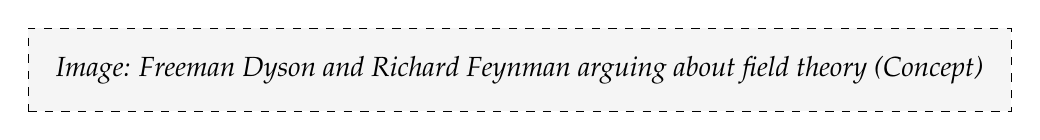
\begin{tikzpicture}
        \node[draw, dashed, inner sep=10pt, fill=theorygray] {
            \textit{Image: Freeman Dyson and Richard Feynman arguing about field theory (Concept)}
        };
    \end{tikzpicture}
\end{center}

In the summer of 1948, two travelers stranded at an inn in Vinita, Oklahoma, due to a flood, spent the night arguing.

\begin{fancyquote}
    \textit{``Dick didn't trust my mathematics, and I didn't trust his intuition... I couldn't imagine that the path integral picture... could hold for electrons but not for gravity... It was a unified theory that either explained everything or nothing. And that made me deeply skeptical. I knew how many great scientists had pursued the firebrand of unified theory. The ground on which science stood was littered with the corpses of dead unified theories... No one but Dick could use his theory... I couldn't call it a theory.''} \\
    --- Freeman Dyson, \textit{Disturbing the Universe}
\end{fancyquote}

This story dates to when only one person in the world could use the path integral method. Richard Feynman had the vision that it could even unify gravity. However, if gravity is nonlinear, standard superposition fails, and background dependence makes the task seemingly impossible. Does Heim's discrete geometry offer a way out?

\subsection{19. Multivariate Metron Functions}
Let $\varphi(n_i)_1^L = \varphi(n_1 \dots n_L)$ be an $L$-dimensional metron function where:
\begin{equation}
    1 \leqq i \leqq L < \infty, \quad 1 \leqq \kappa_i \leqq n_i \leqq N_i < \infty \tag{M9}
\end{equation}

\subsection{20. Partial Derivative}
The partial metron derivative $\eth_i$ with respect to the $i$-th variable is:
\[
    \eth_i \varphi = \varphi - \varphi(\dots, n_i-1, \dots)
\]
The total derivative is the sum of partials: $\eth = \sum_{i=1}^L \eth_i$.

\subsection{21. Commutativity}
The order of metron partial derivatives is interchangeable:
\begin{equation*}
    (\eth_i \times \eth_k)_- = 0, \quad \text{where } (a \times b)_\pm = ab \pm ba
\end{equation*}
This implies $\eth_i \eth_k - \eth_k \eth_i = 0$.

\subsection{22. Composite Functions}
For $\varphi = \varphi(\Psi_1 \dots \Psi_\lambda)$ where $\Psi_j = \Psi_j(n_1 \dots n_L)$:
\begin{equation}
    \eth \varphi = \sum_{j=1}^{\lambda} \eth_{\Psi_j} \varphi \eth \Psi_j, \quad \eth_{\Psi_j} \varphi = (\varphi - \varphi(\dots, \Psi_j - \eth \Psi_j, \dots))(\eth \Psi_j)^{-1} \tag{M9a}
\end{equation}
(Note: Chain rules are rarely used because the discrete processes $\eth$ must usually be carried out separately.)

\subsection{23. Multiple Integrals}
Extension of the metron integral to $L > 1$:
\begin{equation}
    \phi = S_{1+\kappa_1}^{N_1} \dots S_{1+\kappa_L}^{N_L} \varphi(n_i)_1^L \prod_{k=1}^L \eth n_k, \quad \eth_i n_k = \delta_{ik} \tag{M10}
\end{equation}
where $\delta_{ik}$ is the Kronecker delta.

\subsection{24. Convergence and Limits}
A metron function $\varphi$ converges to a limit $g$ if for any $\varepsilon > 0$, there exists a large number $N(\varepsilon) > 0$ such that for all $n_i, n'_i > N$:
\begin{equation*}
    |\varphi(n_i)_1^L - \varphi(n'_i)_1^L| < \varepsilon, \quad |\varphi(n_i)_1^L - g| < \varepsilon
\end{equation*}
We write this as $\lim_{(n_i)_1^L \to \infty} \varphi = g$.

\subsection{25. Sequential Limits}
If a limit exists, the sequential limits must also satisfy convergence:
\begin{equation*}
    \lim_{n_1 \to \infty} \varphi = \varphi_1(n_i)_2^L \dots \lim_{n_L \to \infty} \varphi(n_L) = g
\end{equation*}

\subsection{26. Commutativity of Limits}
In the discrete implementation of limit ordering, the ordering of individual limits $n_i \to \infty$ must commute. If this were not the case, the convergence or divergence of the metron function could not be uniquely explained.
(\textit{Note: The convergence to $\tau \to 0$ suggests Heim is considering the bridge back to calculus-based theory.})

\subsection{27. Homogeneous Metron Functions}
A metron function $\varphi$ is homogeneous of integer degree $h \geqq 1$ if for any integer $t \geqq 1$:
\begin{equation*}
    \varphi(t, n_i)_1^L = t^h \varphi(n_i)_1^L
\end{equation*}
This allows for a metronic relation analogous to Euler's theorem: $\sum x_i \frac{\partial f}{\partial x_i} = hf$.

\subsection{28. Euler Analogy for Metrons}
For integers $\eta_i = n n_i$:
\begin{equation*}
    \eth_n \varphi = \sum_{i=1}^L n_i \eth_{\eta_i} \varphi(\eta_i)_1^L
\end{equation*}
Using binomial expansion for $(n-1)^h$:
\begin{equation*}
    \eth_n \varphi = (-1)^{h+1} \sum_{\nu=0}^{h-1} (-1)^\nu \binom{h}{\nu} n^\nu \varphi(n_i)_1^L
\end{equation*}
Equating the two yields:
\begin{equation*}
    \sum_{i=1}^L n_i \eth_{\eta_i} \varphi(\eta_i)_1^L = (-1)^{h+1} \sum_{\nu=0}^{h-1} (-1)^\nu \binom{h}{\nu} n^\nu \varphi(n_i)_1^L
\end{equation*}

\subsection{29. Positive and Negative Symmetry}
By setting the parameter $n = \pm 1$ (where $\eta_i = \pm n_i$ and $\eth_{\eta_i} = \pm \eth_i$):
\begin{equation*}
    \pm \sum_{i=1}^L n_i \eth_i \varphi(n_i)_1^L = (-1)^{h+1} \varphi \sum_{\nu=1}^{h-1} \binom{h}{\nu} (\mp 1)^\nu
\end{equation*}

\subsection{30. Homogeneity of Metronic Derivatives}
A metron derivative $\eth \varphi$ of a homogeneous function $\varphi$ of degree $h$ is generally \textit{not} homogeneous of degree $h-1$ because derivatives of powers are polynomials (unlike calculus).
However, if $\varphi$ is expressed in the form:
\begin{equation*}
    \varphi = \sum_{j=1}^{\binom{L}{h}} S_j, \quad S_j \sim \prod_{a=1}^h n_a
\end{equation*}
(where no $n_i$ occurs with a power $>1$), then all metron derivatives of degree $k$ are homogeneous of degree $h-k$ for $0 \leqq k \leqq h-1$.

\subsection{31. Conserved Quantities}
If an implicit connection exists in the form $F(\varphi, n_i)_1^L = \text{const}$, then $\eth F = 0$. This expands as:
\begin{equation*}
    \eth_\varphi F + \sum_{i=1}^L \eth_i F = 0
\end{equation*}
If $\eth_\varphi F \sim \eth \varphi$, then the metron derivative $\eth \varphi$ can be extracted. If $\eth \varphi = 0$, then $f(0, \varphi, n_i)_1^L = 0$.

\hr

\begin{reflectionbox}[title={Notes and Reflections: The Deciphering Task}]
This is undeniably hard to read. The original formulas and explanations are almost one-dimensional, with few line breaks. Deciphering where one operation ends and the next begins is a task in itself.

We have completed Chapter 3, Part 1 (Basic Metron Operations). It is a foundation built on the rejection of the infinitesimal in favor of finite area elements. Next time, we look at the ``Selector.'' What could that be?
\end{reflectionbox}

\begin{sectionrefs}
    \item \href{https://en.wikipedia.org/wiki/Path_integral_formulation}{Path Integral Formulation}: Context for the discussion between Feynman and Dyson.
    \item \href{https://en.wikipedia.org/wiki/Freeman_Dyson}{"Disturbing the Universe"} by Freeman Dyson: Source for skepticism regarding unified field theories.
    \item \href{https://en.wikipedia.org/wiki/Homogeneous_function}{Homogeneous Function}: Concept applied to multivariate metron functions.
\end{sectionrefs}

\hr

\subsection*{In-Depth: The 6D Coordinate Space (Map III-2)}
\addcontentsline{toc}{subsection}{In-Depth: The 6D Coordinate Space}

Multivariate analysis in Metron Calculus is specifically designed to handle the **6-dimensional manifold** ($L=6$). Heim’s logic dictates that if the fundamental unit is a surface, then the dimensions must be the number of planes in an underlying geometry.

\subsubsection*{1. The Plane-Based Geometry}
In a standard $N$-dimensional space, the number of independent surface elements (planes) is $L = \binom{N}{2}$.
\begin{itemize}
    \item For $N=4$ (Space-time), $L = \binom{4}{2} = 6$.
\end{itemize}
The multivariate metron function $\varphi(n_i)_1^L$ described in Section 19 is thus the standard description of a 6-dimensional state in $R_6$. Each integer argument $n_i$ represents the count of metrons ($\tau$) in one of the 6 fundamental planes.

\subsubsection*{2. The Eigenvalue Mapping}
Sections 27 and 28 (Euler Analogy) are the mathematical precursors to the **Selector Equations**. Heim uses the homogeneity of these functions to prove that a discrete field can satisfy a relation analogous to the linear operators of quantum mechanics:
\begin{equation}
    \sum_{i=1}^L n_i \eth_i \varphi = \lambda \varphi
\end{equation}
This allows Heim to treat the entire universe as a system of eigenvalue equations. If $\lambda$ is an integer, the structure is stable. This is the "Selector" mechanism: the geometry \textit{selects} only those states where the multivariate sum of metron differences reaches an integer resonance.

\subsubsection*{3. Resolving the Divergence "Blemish"}
In Part 3, Heim mentioned that his unified energy tensor had non-zero divergence ($T^{ik}_{;k} \neq 0$) in 4D. Section 31 (Conserved Quantities) provides the hint to the solution:
\begin{mbbcite}
    \textbf{The Dimensional Shift:} A quantity that appears to vary in 4 dimensions (having non-zero divergence) can be constant ($\eth F = 0$) when analyzed as a multivariate function in the full 6-dimensional manifold. 
\end{mbbcite}
By expanding the analysis to $L=6$, the "missing" energy and momentum terms that caused the divergence in $R_4$ are shown to be geometric flux exchanges between the spatial ($R_3$), temporal ($x_4$), and structural ($x_5, x_6$) dimensions. Conservation is restored globally, even if it is locally violated in the 4D projection. 
% ==============================================================================
% ==============================================================================
\section{Metron Calculations Part 4: Selector Theory I}
% ==============================================================================
\textit{Basic Structure III-2: The Selector}

\subsection{Prologue: Context and Worldview}

The year 2021 began in a state of global turmoil. Some of my colleagues call the equations we are about to study the ``Global Equation.'' I disagree. The term ``World Equation'' is too expansive by definition, as it applies only to the physical realm. Therefore, a more accurate term is the \textbf{World Selector}.

This physics is ultimately just a snippet that we have access to thanks to the structure of our bodies and brains. It is an excerpt from a higher world. To suggest a ``Theory of Everything'' or a ``God’s Formula'' that governs the entire universe might actually indicate a lack of deep reflection. Right now, the concept of a \textit{World Selector} may be difficult to grasp, but it is the key to moving beyond simple background-dependent theories.

\subsection{1. The Selector Concept}

Since the argument $n_i$ is an integer, the metron function $\varphi(n_i)_1^L$ can be viewed as an $L$-dimensional array. In this context, $\varphi$ is a substitution rule that selects a sequence from a corresponding algebraic number field. A change in $\varphi$ implies a change in the structure of the array.

The quantity that modifies these substitution rules is defined as an \textbf{operator}, which in metron calculus is called a \textbf{Selector}.

\textbf{Example:} In Lesson 23, we saw that for a homogeneous function of degree $h$:
\begin{equation*}
    \sum_{i=1}^L n_i \eth_i \varphi = \lambda \varphi
\end{equation*}
We can define the left-hand side operator as $C$. Using the selector notation, where the symbol ``;'' denotes that the selector acts on a function:
\begin{equation}
    C; \varphi = \lambda \varphi
\end{equation}
This notation distinguishes the selector from a standard differential operator. Every metron function $\varphi$ can be expressed as a sequence of selectors acting on a sequence of positive integer metron numbers $n_i > 0$.

\subsection{2. Assignment Selectors (\textit{Zuordnungsselektors})}
The assignment selector $Z(i)$ selects a specific component:
\begin{equation*}
    Z(i) = (\ )_i, \quad Z(i); n = n_i
\end{equation*}
Thus, $\varphi(n_i)_1^L = \varphi(Z(i); n)_1^L$.

\subsection{3. Function Selectors (\textit{Funktionalselector})}
If $L$ adjustment selectors (\textit{Koordinationsselektoren}) are linked by $K$ selectors $C_k$, the action on the entire sequence $n$ generates the metron function $\varphi$:
\begin{equation}
    Z(i) = (\ )_i, \quad \varphi(n_i)_1^L = \phi; n, \quad \phi = \phi(C_k, Z(i))_{i,k=1}^{L,K}, \quad C_k; n_i = f_k(n_i) \tag{M11}
\end{equation}
We distinguish between adjustment selectors (which act as arguments) and function selectors (like $C_k$ and the associative selector $\phi$).

\subsection{4. Zero Selector (\textit{Nullselektor})}
\begin{equation*}
    0; n = 0
\end{equation*}

\subsection{5. Identity Selector (\textit{Einheitsselektor})}
\begin{equation*}
    E; n = 1, \quad E; (\ ); n = n
\end{equation*}

\subsection{6. Algebraic Properties}
Selectors satisfy associative and distributive laws with respect to addition and multiplication. However, the \textbf{commutative law applies only to addition}. For multiplication, the order matters:
\begin{equation*}
    (C_i \times C_k)_{\pm} \neq 0
\end{equation*}
Since differentiation and integration are themselves function selectors, commutators and anticommutators often exist and are non-zero.

\subsection{7. Constant Selector}
For all $n$ where $n=a$ (constant):
\begin{equation}
    C; n = a = \text{const}(n), \quad C = a \frac{(\ )}{(\ )} \tag{M11a}
\end{equation}

\subsection{8. Metron Vectors}

In Heim's theory, every metron region $n_i$ must have dimension $p$ based on the geometric interpretation of $\tau$. To metronize coordinates $x_i$ ($1 \le i \le L$) in $R_L$ with $R_p$ ($p \le L$), we extend the adjustment selector to a \textbf{directional adjustment selector} (\textit{orientierten Koordinationsselektor}):
\begin{equation}
    \bar{Z}(i) = \bar{e}_i (\ )_i, \quad | \bar{e}_i | = 1, \quad (\bar{e}_i, \bar{e}_k)_L = \hat{A}(n_i)_1^L \tag{M11b}
\end{equation}
Here, $\bar{e}_i$ is an $L$-th order square matrix. Note that these are not necessarily orthogonal; in general, $\hat{A} \neq \hat{E}$.

\subsection{9. Metron Vector Fields}
A general metron vector field on an $L$-dimensional argument is described by the function selector $\bar{C}$ oriented by $\bar{\varphi}$:
\begin{equation*}
    \bar{\varphi} = \bar{C}; n, \quad \bar{C}_i = \bar{e}_i C_i
\end{equation*}
This metron vector can be understood as a first-order metron tensor.

\subsection{10. Metron Tensors}
For a tensor order $m \ge 1$, the metron tensor ${}^m \bar{T}$ is defined by components $T_{i_1 \dots i_m}$ constructed from vector components:
\begin{equation}
    T_{i_1 \dots i_m} = \prod_{k=1}^m \varphi_{i_k} = \left( \prod_{k=1}^m C_{i_k} \right); n \tag{M11c}
\end{equation}
The tensor function selector is given by:
\begin{equation*}
    {}^m \bar{C} = {}^m [ \prod_{k=1}^m C_{i_k} ]_L, \quad {}^m \bar{T} = {}^m \bar{C}; n, \quad 0 \le m \le L
\end{equation*}
When $m=0$, we return to a metron scalar function.

% --- DIAGRAM REPLACEMENT FOR heim_buildchart.jpg ---
\begin{center}
    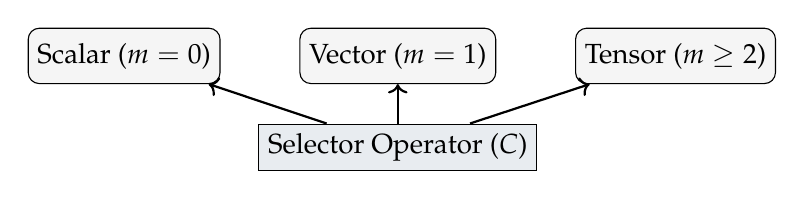
\begin{tikzpicture}
        \node[process] (scalar) {Scalar ($m=0$)};
        \node[process, right=of scalar] (vector) {Vector ($m=1$)};
        \node[process, right=of vector] (tensor) {Tensor ($m \ge 2$)};
        
        \node[draw, rectangle, below=0.5cm of vector, fill=theoryblue!10] (selector) {Selector Operator ($C$)};
        
        \draw[->, thick] (selector) -- (scalar);
        \draw[->, thick] (selector) -- (vector);
        \draw[->, thick] (selector) -- (tensor);
    \end{tikzpicture}
    \captionof{figure}{Hierarchical Structure of Selectors acting on Metron Functions.}
\end{center}

\begin{sectionrefs}
    \item \href{https://en.wikipedia.org/wiki/Selector}{Selector (Mathematics)}: Definition for the metron operator $C$ acting on metron functions $\varphi$.
    \item \href{https://en.wikipedia.org/wiki/Kronecker_delta}{Kronecker Delta}: Used in defining constant and identity selectors.
    \item \href{https://en.wikipedia.org/wiki/Torsion_tensor}{Torsion Tensor}: Geometric context for the non-commutative nature of selector multiplication.
\end{sectionrefs}

\hr

\subsection*{In-Depth: The Logical Structure of Selector Theory (Map III-2)}
\addcontentsline{toc}{subsection}{In-Depth: The Logical Structure of Selector Theory}

Selector theory is the mathematical framework required to process physics in a discrete, $L$-dimensional metron manifold. It replaces the infinitesimal coordinate differentials of Einstein with **State Selection Operators**.

\subsubsection*{1. Coordination and Aspect (Eq. M11b)}
Heim defines the metric structure of the world through the **Orientation Matrix** $\hat{A}$.
\begin{equation}
    (\bar{e}_i, \bar{e}_k)_L = \hat{A}(n_i)_1^L
\end{equation}
If $\hat{A} = \hat{E}$ (Identity matrix), the space is an orthogonal, Euclidean metron grid. If $\hat{A}$ varies with the metron digits $n_i$, the space is curved. Crucially, in Heim's theory, the "Metric" is not a background but an **Assignment Selector** ($Z$). Space does not exist as a container; it is selected by the interrelationship of metron digits.

\subsubsection*{2. The Non-Commutativity of the World Selector}
As stated in Section 6, selectors do not generally commute: $[C_i, C_k] \neq 0$. In Heim's geometry, this is the origin of physical fields. 
\begin{itemize}
    \item **Gravitation:** Corresponds to the symmetric part of the selector product.
    \item **Electromagnetism:** Corresponds to the anti-symmetric (non-commutative) part.
\end{itemize}
By using selectors, Heim avoids the "Wood vs. Marble" problem. The mass and charge of a particle are not "added" to the geometry; they are the result of specific **Function Selectors** ($\phi$) that "select" a stable, non-Euclidean configuration from the number field.

\subsubsection*{3. Constructing the Metric Tensor (Eq. M11c)}
The macroscopic metric tensor $g_{ik}$ is derived from the second-order tensor selector ${}^2 \bar{C}$.
\begin{equation}
    g_{ik} = {}^2 \bar{C}; n = (C_i \cdot C_k); n
\end{equation}
This confirms that the metric itself is quantized. Every "point" in the macro-world is actually a cluster of 36 metron states selected by the 6D tensor operator. This is the bridge between the discrete integer arguments of the microcosm and the continuous tensor fields of General Relativity. 
% ==============================================================================
% ==============================================================================
\section{Metron Calculations Part 5: Selector Theory II}
% ==============================================================================
\textit{Heim's elementary particle mass formula 25: Metron calculation part 5 \\ - Selector part 2 -}

\hr

\subsection{11. Orientation Matrix and Tensor Analysis}
According to the properties of the tensor selector ${}^m \bar {C}$ (M11a), the orientation matrix $\hat {A} = \hat {A}(n_i)_1^L$ may also be a metron function, which allows for metron tensor analysis and justification of the metron theory of metron tensor systems. However, to run this program, it is necessary to analyze the properties of the tensor selector ${}^m \bar {C}$.

\subsection{12. Transpose and Component Notation}
The components $C_{i_k ... i_m} = \prod_{k = 1} ^m C_{i_k}$ of the transpose ${}^m \bar {C}$ have index $1 \leqq l \leqq m$, and using the notation $C_{i_l} = C_{l}$ it is possible to express:
\begin{equation*}
\prod_{k = 1}^{l-2} C_{i_k}; C_{l-1}; C_{l}; \prod_{ k = l + 1}^m C_{i_k}
\end{equation*}
(The selector effect is similar to multiplication, so the symbol $\prod$ is only formal.) Performing a transpose $T$ with indices $l-1$ and $l$ gives us the component notation of ${}^m \bar {C}^{T\ l-1,l}$:
\begin{equation*}
C_{i_1 ... i_m}^{T\ l-1,l} = \prod_{k = 1}^{l-2} C_{i_k};C_{l};C_{l-1}; \prod_{k = l + 1}^m C_{i_k}
\end{equation*}

\subsection{13. Hermitian and Anti-Hermitian}
On the other hand, as in tensor analysis:
\begin{equation*}
{}^m \bar {C}_{ \pm(l-1,l)} = \frac {1} {2}({}^m \bar {C} \pm {}^m \bar {C}^{\times l-1,l} )
\end{equation*}
We can Hermitize or anti-Hermitize with $(\pm)$ of $l-1,l$. (Symmetrization or antisymmetrization is referred to in component notation). 

\begin{fancyquote}
    \textbf{9th Lecture: On the terms Hermitian and symmetric: (k)}
\end{fancyquote}

\begin{align*}
2C_{\pm(l-1,l)i_1 ... i_m} &= C_{i_1 ... i_m} \pm C_{i_1 ... i_m}^{Tl-1,l} \\
&= \prod_{k = 1}^{l-2} C_{i_k}; C_{l-1}; C_l;\prod_{k = l + 1}^m C_{i_k } \pm \prod_{k = 1}^{l-2} C_{i_k}; C_l; C_{l-1}; \prod_{k = l + 1}^m C_{i_k} \\
&= \prod_{k = 1}^{l-2} C_{i_k}; (C_{l-1}; C_l \pm C_l; C_{l-1}); \prod_{k = l + 1}^m C_{i_k} \\
&= \prod_{k = 1}^{l-2} C_{i_k};(C_{l-1} \times C_l)_{\pm}; \prod_{k = l + 1}^m C_{ i_k}
\end{align*}

If $C_{i_k} = C_{i_k}^{*}$, that is, depending on whether the two partial selectors to be transposed have anticommutators or commutators different from the zero selector, a symmetric or antisymmetric form exists. If $C_{i_k} \neq C_{i_k}^*$, the corresponding algebraic investigation can be performed in the complex field with the help of adjoint matrices, but the simple notation with anticommutators or commutators is omitted.

The general case can be reduced to $m = 2$ without restricting general validity. Therefore, the symmetry investigation of tensor selectors always follows the scheme:
\begin{equation}
    {}^2 \bar {C} = [C_i; C_k)_{\pm}]_L,\quad {}^2 \bar {C}_+ = {}^2 \bar {C}_+^x,\quad {}^2 \bar {C}_- =-{}^2 \bar {C}_-^x \tag {M12}
\end{equation}
According to this, for real numbers, ${}^2 \bar {C}_{\pm } = {}^2 \bar {0}$ applies whenever $(C_i \times C_k)_{\pm } = 0$, regardless of whether $m = 2$ or $m > 2$ applies.

\subsection{14. Trace (Spur)}
\begin{fancyquote}
    \textbf{(Note)} Notational Differences: (English) trace, (German) spur. $tr \bar{C} \equiv \spn \bar{C}$. In Heim's materials, the sp notation is standard. (k)
\end{fancyquote}

Another important operation of tensor selectors is the contraction of tensors by forming matrix traces. For $C_{i_j} = C_j$ and $C_{i_l} = C_l$, ${}^m \bar {C}$ forms a matrix trace with $j = l$ and the sum over all $1 \leqq l \leqq L$, $m$ decreasing by 2.

In general:
\begin{equation*}
    \spn_{j = l} {}^m \bar {C} = \{^{[m-2]} [\sum_{l = 1}^L \prod_{k = 1}^{j-1}; C_{i_k}; C_l; \prod_{k = j + 1}^{l-1}; C_{i_k};C_l; \prod_{k = l + 1}^{m }; C_{i_k}]_L = {}^{m-2} \bar {C}
\end{equation*}
Again, we can reduce to $m = 2$ without loss of generality. This effectively gives:
\begin{equation}
    \spn {}^2 \bar{C} = \sum_{i = 1}^L C_i^2,\quad \spn_{i = k} {}^m \bar{C}_{+(i,k)} = {}^{m-2} \bar{C},\quad \spn_{i = k} {}^m \bar{C}_{-(i,k)} = {}^{m-2} \bar{0} \tag{M12a}
\end{equation}

\subsection{15. Tensor and Scalar Actions}
For tensor selectors of rank $m \geqq 1$, the directed function selector $\bar{D}$ can act.
\begin{itemize}
    \item \textbf{Tensor Action:} If the result is $W$, then $\bar{D};{}^m \bar{C} = {}^{m + 1} \bar{W}$ always provides an expansion of the tensor rank.
    \item \textbf{Scalar Action:} If $\bar{D}$ is an oriented function selector, then $\spn \bar{D};{}^m \bar{C} = {}^{m-1} \bar{W}$ characterizes a scalar action.
\end{itemize}
An oriented function selector expands the tensor rank by one for tensor actions, but a scalar action, being a matrix trace of a tensor action, reduces the tensor rank by one. On the other hand, if the function selector is not oriented ($D$), then $D;{}^m \bar{C} = {}^m \bar{W}$ (no rank change).

\subsection{16. DIV, ROT, GRAD - Analogies of Vector Analysis}
The special form of $\bar{D}$, $\bar{D} = \bar {\ethop} = \sum_{i = 1}^L \bar {e_i}\ethop_i$, is analogous to an infinitesimal tensor divergence in the case of a tensor action and to a scalar divergence in the case of a scalar action.

Therefore, this tensor, scalar, and indifferent \textit{Einwirkung} (influence) of function selectors on tensor selectors with the special case $\bar {\ethop}$ is:
\begin{equation}
    \begin{gathered}
    \bar {D}; {}^m \bar {C} = {}^{m + 1 } \bar {W},\quad \spn \bar {D}; {}^m \bar {C} = {}^{m-1} \bar {W},\quad D; {}^m \bar {C} = {}^m \bar {W} \\
    \bar {\ethop} = \sum_{i = 1}^L \bar {e_i}\ethop_i,\quad \bar {\ethop} \varphi = \mathrm{GRAD_L} \varphi,\quad \bar {\ethop}; {}^m \bar {C} = \widehat{\mathrm{DIV_L}} {}^m \bar {C} \\
    \spn \bar {\ethop}; {}^m \bar{C} = \overline{\mathrm{DIV_L}} {}^m \bar {C},\quad\bar{\ethop}; {}^m \bar {C}-(\bar{\ethop}; {}^m \bar {C})^x = \mathrm{ROT_L} {}^m \bar {C} 
    \end{gathered} \tag {M12b}
\end{equation}
and the metronic counterparts of the infinitesimal tensor analytical differential operators are symbolized in the manner described above.

\subsection{17. Properties of DIV, ROT, and GRAD}
Since each of these selectors represents a metronic equivalent of an infinitesimal operator, metronic theorems can also be extended for these selectors. For example, if $Im\mathrm{ROT_L} = {}^2 \bar {0}$, then $\mathrm{ROT_L} = -(\mathrm{ROT_L})^x$, and therefore $\spn\mathrm{ROT_L} = 0$.

Furthermore, in the component representation:
\begin{equation*}
    (\widehat{\mathrm{DIV_L}} \mathrm{ROT_L})_{ikl} = \ethop_i(\ethop_k()_l-\ethop_l()_k) \neq 0
\end{equation*}
Repeating the divergence formation and using $\sum \ethop()_i = \mathrm{DIV_L}()$:
\begin{align*}
    (\overline {\mathrm{DIV_L}}\mathrm{ROT_L})_l &= \sum_{i = 1}^L\ethop_i(\ethop_i()_l-\ethop_l()_i) \\
    &= \sum_{i = 1}^L\ethop_i^2()_l- \sum_{i = 1}^L\ethop_l\ethop_i()_i \\
    &= \mathrm{DIV_L} \mathrm{GRAD_L}()_l-(\mathrm{GRAD_L})_l\mathrm{DIV_L}()
\end{align*}
Finally, we can derive another theorem for metron rotation. The combined selector $\mathrm{ROT_L}\mathrm{GRAD_L}$ obviously acts only as a second-order tensor selector in metronic scalar fields, but its component representation implies $(\ethop_i\times\ethop_k)_- = 0$.

Therefore, it applies to these special selectors in (M12b):
\begin{equation}
    \begin{gathered}
    Im\mathrm{ROT_L} = {}^2 0,\quad \spn\mathrm{ROT_L} = 0, \\
    \overline{\mathrm{DIV_L}}\mathrm{ROT_L} = \mathrm{DIV_L}\mathrm{GRAD_L}-\mathrm{GRAD_L}\mathrm{DIV_L}, \\
    \mathrm{DIV_L} \overline{\mathrm{DIV_L}}\mathrm{ROT_L} = 0,\quad \mathrm{ROT_L}\mathrm{GRAD_L} = {}^2 0 
    \end{gathered} \tag {M12c}
\end{equation}

\subsection{18. Some Metron Integral Theorems}
Correspondingly, we can also develop some Metron integral theorems. If $\ethop\bar {N} = \sum_{i = 1}^L \bar {e_i}\ethop_i()_i$, and assuming a normalized orthogonal system $\hat{E}$, the formation of the metron integral is possible.

The Metron integral theorem states that the system:
\begin{equation}
    \begin{gathered}
    S(\mathrm{GRAD_L} \phi \ethop\bar {N}); n = \rm{const},\quad S_{\Omega(L)} \mathrm{DIV_L} \bar {\phi}\ethop V = S_{\Omega(L-1)} \bar {\phi}\ethop\bar {V}, \\
    SS \mathrm{ROT_L} \bar {\phi}\ethop^2 \bar {F} = S \bar {\phi}\ethop\bar {N},\quad \ethop\bar {N} = \sum_{i = 1}^L\ethop_i\bar {Z}(i), \\
    \ethop V= \prod_{k = 1}^L\ethop_kZ(k),\quad \ethop\bar {V} = \sum_{j = 1}^L \bar {e}_j\ethop V_j , \\
    \ethop V_j= \prod_{k = 1}^{j-1}\ethop_kZ(k)\prod_{j + 1}^L\ethop_kZ(k),\quad (\bar {e}_i \bar {e }_k)_L = \hat {E}, \\
    \ethop^2 \bar {F} = [\ethop_iZ(i)\ethop_kZ(k)]_L 
    \end{gathered} \tag {M13}
\end{equation}

\subsection{20. Selector Equations for the Fibonacci Sequence}
For example, we have a Fibonacci sequence of the form $a_n = a_{n-1} + a_{n-2}$.
The conditions $\varphi(n) = \varphi(n-1) + \varphi(n-2)$ allow us to interpret all sequences of digits $a_n = \varphi(n)$ as metronome functions. From this, we can derive selectors for these sequences. This is called a \textbf{construction selector}.

From $\varphi(n)= \varphi(n-1)+ \varphi(n-2)$, we immediately get $\varphi(n-2)= \varphi(n)-\varphi(n-1)=\ethop\varphi$.
The second metronome derivative $\ethop^2 \varphi = \ethop(\varphi- \varphi(n-1))=\ethop\varphi-\ethop\varphi(n-1)= \ethop\varphi- \varphi(n-1)+ \varphi(n-2)$. Substituting in $-\varphi(n-1)=\ethop\varphi- \varphi$ and $\varphi(n-2)=\ethop\varphi$ yields $\ethop^2 \varphi =3\ethop\varphi-\varphi$.
Or we use $\ethop^2 \varphi-3\ethop\varphi + \varphi = 0$ as the selector equation, so the creation selector $\ethop^2 -3\ethop +()= 0$ is applied.

Since the sequence is monotonically increasing, there must exist limiting values $\xi$.
\begin{equation*}
    \xi = \lim_{n \to \infty} \varphi(n)/ \varphi(n-1) = 1 + 1 / \xi
\end{equation*}
That is, the limit values can be determined from the quadratic equation $\xi^2- \xi = 1$ under the condition $\xi > 1$. We obtain two solutions $2 \xi_{\pm} = 1 \pm \sqrt {5}$.

Therefore, the creation selector and its function constraint are:
\begin{equation}
    \ethop^2-3\ethop+()= 0,\quad 2 \xi = 1+ \sqrt {5} \tag {M14}
\end{equation}
This describes the Fibonacci sequence.

\hr

\begin{reflectionbox}[title={Chat / Notes}]
    \textbf{11-12.} It's unusual to explicitly state the tensor order (rank) on the left shoulder (usually, it's not explicitly written because it can be determined by the number of subscripts. I wonder if there's any benefit to it?) If ${}^2\bar{0}$, then in L dimensions, all $L^2$ components are zero.
    
    \textbf{13-14.} *0 I don't understand the meaning. Q.18 What does ``Simple notations using anticommutators or commutators are omitted'' mean?
    
    \textbf{*1 Trace component notation:} 
    Added correction: $1 \leqq l \leqq L \to 1 \leqq i \leqq L$. The meaning of $sp_{j=l}$ being equal doesn't make sense. It could be the meaning of $i=k$ in $\sum_{i=k=1}^L C_{ij}C_{kl}$.
    Correction: $sp_{j = l} {}^m \bar {C} = \{^{[m-2]} [\sum_{l = 1}^L \prod_{k = 1}^{j-1}; C_{i_k}; \underline{C_j}; \prod_{k = j + 1}^{l-1}; C_{i_k};C_l; \prod_{k = l + 1}^{m }; C_{i_k}]_L = {}^{m-2} \bar {C}$.
    The underlined part of this equation seems to mean that $C_l \to C_j$ is the correct $sp_{j=l}$ and contraction is performed using the jth and lth subscripts...
    
    \textbf{16-18.} * What the heck?! I was dazed for a moment, but it seems that Professor Heim wanted to create an L-dimensional tensor selector version of the integral theorem of vector analysis.
    
    \textbf{Example:} The divergence of an electric field vector (a 1st order tensor) is proportional to the scalar quantity called electric charge (a 0th order tensor). Let's compare:
    $\mathrm{rot}\mathrm{grad} \phi =0 \iff \mathrm{ROT_L}\mathrm{GRAD_L} = {}^2 0$. This is exactly the same.
    
    The good news from Part 5 echoes in my head: ``For example, we cannot expect Maxwell's equations to completely describe the properties of the electromagnetic field...'' ``Yes, that's what I wanted to hear!''
    
    \textbf{Gauss's theorem:}
    $\iiint_V \mathrm{div} \vec{A}dV = \iint_S \vec{A} \cdot dS \iff S_{\Omega(L)} \mathrm{DIV_L} \bar {\phi}\ethop V = S_{\Omega(L-1)} \bar {\phi}\ethop\bar {V}$
\end{reflectionbox}

\hr

\subsection*{In-Depth: The Eigenvalue Mapping in $R_6$ (Map II-1 Detailed)}
\addcontentsline{toc}{subsection}{In-Depth: The Eigenvalue Mapping in $R_6$}

Heim utilizes the multivariate selector calculus to define the microscopic curvature of the $R_6$ manifold. This replaces the three-index Christoffel symbol $\Gamma^i_{km}$ with a metric state function $\phi^i_{km}$.

\subsubsection*{1. The Curvature Step Operator}
The curvature steps of the curved $R_6$ are defined by the action of the functional operator $C_p$ on the state function:
\begin{equation}
    C_p \phi^i_{km} = \lambda_p(k, m) \phi^i_{km} \tag{II-1.3}
\end{equation}
To mathematically prove that these curvature steps correspond to real, observable physical states, Heim introduces the normalized state function $\Psi$ (where $\int \Psi\Psi^* d\Omega = 1$) and maps the geometric operators to Hermitian linear operators $H_{km}^{(p)}$ and $L_{km}^{(p)}$:
\begin{equation}
    H_{km}^{(p)}\Psi = h_{km}^{(p)}\Psi \quad \text{and} \quad L_{km}^{(p)}\Psi = l_{km}^{(p)}\Psi
\end{equation}
Because $H$ and $L$ are Hermitian, their eigenvalues are strictly real ($h = h^*$ and $l = l^*$). Setting the proportionality $H_{km}^{(p)} \sim L_{km}^{(p)}$, Heim establishes the approach:
\begin{equation}
    H_{km}^{(p)}\Psi = \lambda_{(p)}(k,m)L_{km}^{(p)}\Psi
\end{equation}
Integrating this over the space-time volume $\Omega$ yields the definitive proof:
\begin{equation}
    0 = \int \left( \Psi^* H_{km}^{(p)}\Psi - \Psi(H_{km}^{(p)}\Psi)^* \right) d\Omega \implies 0 = \lambda_{(p)}(k,m) - \lambda_{(p)}(k,m)^*
\end{equation}
This proves $\lambda_{(p)}(k,m) = \lambda_{(p)}(k,m)^*$. The curvature steps $\lambda_{(p)}$ are strictly real and symmetrical. They form discrete point spectra, meaning the fabric of $R_4$ curves in exact, quantum-like energy steps.
Here, the operator $C_p$ performs the role of the metronized covariant derivative. The eigenvalues $\lambda_p$ represent the discrete quanta of curvature that exist in the $R_6$ lattice. 

\subsubsection*{2. The Reduction of the 64 Equations}
As noted in the text, there are $4 \times 4 \times 4 = 64$ nonlinear tensorial equations at the start of the derivation. Heim uses the anti-Hermitian symmetries of the selector transpose (Section 13) to identify empty spectra.
\begin{itemize}
    \item By requiring the trace of the microscopic operator to vanish ($C_m \phi^k_{km} = 0$), Heim identifies **28 empty spectra** (Relation 3a in Map II-1).
    \item This leaves $64 - 28 = 36$ occupied energy levels. 
\end{itemize}
The $6 \times 6$ tensor matrix is the only structure capable of holding these 36 non-zero states. This proves that the material world \textit{cannot} be described by 4 dimensions; the discrete eigenvalue spectrum forces a 6-dimensional stage.

\subsubsection*{3. Stability and "Marble"}
The construction selector (Section 20) applied to the Fibonacci sequence is a simplified example of the **World Selector**. Just as the Fibonacci sequence has a stable limit value $\xi = (1+\sqrt{5})/2$, the material field quanta have stable mass levels defined by the zeros of the World Selector. This turns Einstein's "wood" into "marble": matter is not an input, but the stable resonance of a discrete geometry.
% ==============================================================================
% ==============================================================================
\section{Metron Calculations Part 6: Primitive Structure Tensors I}
% ==============================================================================
\textit{Heim's elementary particle mass formula 26: Metron calculation Part 6 \\ - Selector theory of primitive structure tensors (Part 1) -}


\begin{reflectionbox}[title={Translator's Note: The Edge of the Continuum}]

\textbf{Q.} Do you have any thoughts on what you've done so far? \\
\textbf{A.} Learning the super-convenient "calculus," which was supposed to be a weapon for confronting the "mysteries of the world," was itself a "trap" that trapped my thoughts at the "edge" of the continuum. 

Children who see the square root symbol and feel uncomfortable are surely the ones who are aware of a paralysis of thought. The entrance door to symmetry is where quadratic equations cannot be solved. Perhaps people who somehow stumble at this root have even greater talent. If there are any students reading this, let's keep it a secret until we graduate. Starting from this point, we will begin deciphering Chapter 3, Part 3.
\end{reflectionbox}

\hr

\subsection{3. Selector theory of primitive structure tensors}
Before developing metric theory, we need to investigate the extension of the conceptual formation of the metron tensor and the possible dimensions of the metron tensor. If metrons are given as elements in $R_p$ by $\tau > 0$, then these metrons are enclosed by a $(p-1)$-dimensional hypersurface, and these hypersurfaces together with the family parameter $t$ form a Euclidean hypersurface family $f(x_i,t)_1^p = 0$ in $R_p$, where the condition for continuous connection of $p$-dimensional metrons $\tau > 0$ is satisfied.

In this way, $R_p$ adjusted to the $t$ value has an integer multiple of $\tau$ for its volume, which results in an integer division of the coordinate $x_i$ according to $x_i(n)$. The integer sequence $n$ runs through the metron domain $1 \leqq n \leqq N$, and the $p$ grids $x_i(n) \hat{=} x_{(i)n}$ can be called a simple primitively structured metron tensor.

\textbf{1.} Such simple tensors are therefore always $p$-dimensional, spanning $p$ coordinates $x_{(i)n}$. These coordinates are arithmetic functions of the integer metron number $n$, serving as a grid of metron numbers. In the explicit case, this is clear because $\int_\omega \prod_{i = 1}^p dx_i = n \tau$. In the implicit case $f(x_i,t)_1^p = 0$, we must eliminate the parameter $t$.
Using the partial derivative $\dot {f} = \frac {\partial f}{\partial t}$, with $df = 0$, i.e., $\sum_{i = 1} ^ p \frac {\partial f}{\partial x_i} dx_i + \dot {f} dt = 0$.
This total differentiation always allows $\prod_{i = 1}^p dx_i$ by eliminating $t$ so that the dimension becomes $p$. Since $\int_\omega \prod_{i = 1}^p dx_i = n \tau$, the grid division $x_{(i)n}$ is preserved even in the implicit case $f = 0$.

\textbf{2.} In the case of general metrics, all these simple metron tensors are Euclidean hypersurfaces $R_p$ in $R_{p + 1}$, but when the family parameter $t$ is introduced as an additional dimension $t = z$, this $R_{p + 1} \equiv V$ can have any metric structure. $f(x_i)_1^{p + 1} = 0$, $z = x_{p + 1}$ is the most general form of a hypersurface in $V$.
The projection onto a $p$-dimensional coordinate hyperplane is performed by equating coordinates not contained in this hyperplane to a parameter. This parameter appears as a family parameter of a $(p-1)$-dimensional hyperplane.

\textbf{3.} If such a projection parameter is $\eta_k$, then we have a projection $f_k(x_i)^p_1 = \eta_k = \text{const}$ of $1 \leqq k \leqq p$. This system of $p$-hypersurfaces described by the $x_i$ domain can also be regularly mapped onto the $\eta_k$ domain if $f_k$ is one-to-one. By metronizing the volume $F = n \tau$ of this hypersurface, we must conclude that $f = 0$ represents a general metric structure for simple metron tensors.
Invariance of metron numbers is obvious because coordinate transformations are changes of aspect.

\subsection{Multidimensionalization}
In this way, every metron function $\varphi(n)$ whose metron argument is one-dimensional can be geometrically interpreted as a state function that assigns to each element—i.e., each metron of a simple tensor denoted by $n$—a metron state value $\varphi$. In addition to the simple sequence $L = 1$, there also exist several sequences $L > 1$. As a result, there exist metron functions $n_i(\xi_{(i) k})^p_1$ that depend on $L$ metron arguments $n_i$. If $\xi_{(i)k}$ in $1 \leqq k \leqq p$ is the geodesic coordinate of a simple tensor $i$, then the arguments characterzie a simple metron tensor, since the dimension of $\tau$ is $p$.

\subsection{Dimensionality Relation}
Equation 15b is the relation when $R_m$ has $p$-dimensional metrons (Basic Structures, Vol. 1, 2-4, p. 95):
\begin{equation}
    m/p = M \geqq 1,\quad (M) \text{MOD}(1) = 0 \tag{15b}
\end{equation}

Each sequence of $L$ metron numbers corresponds to $R_p$ as a multidimensional metron tensor. That is, $R_N$, representing an $L$-dimensional tensor, must be such that it can contain $L$ mutually independent $R_p$ with respect to $N$. The condition for this is $L = \binom {N}{p}$. Since selection rule (15b) applies to $N$, this relation is the selection rule for $L \geqq 1$.

The $L$-dimensional metron argument of $\varphi$ is characterized by its discontinuity, and this metron discontinuity must also characterize $R_N$. In particular, there must be a volume discontinuity in $R_N$, which generates the selection rule $N = pM$ in equation (15b). Substituting $L = \binom {N}{p}$, we obtain the number $L$ of possible simple metron tensors in $R_N$, i.e., $L = \binom {pM}{p}$.

This returns the metron representation of an $L$-dimensional metron tensor in $R_N$ always being:
\begin{equation}
    \varphi(n_i)^L_1 = \varphi(x_k)^N_1,\quad L = \binom {N}{p} \tag{M15}
\end{equation}

\textbf{4.} Thus, the general metron field $\varphi(n_i)^L_1$ on an $L$-dimensional tensor is always a metron state function, assigning a metron state value to each element of $R_N$ represented by $N = pM$. If $1 \leqq k \leqq N$-valued $\xi_k$ represents the geodetic coordinates in the direction $\bar{\xi_k} = \bar{e}_k \xi_k$, then $d \vec {s} = \sum_{k = 1}^N d \vec {\xi}_k$.

\hr

\begin{reflectionbox}[title={Chat / Notes}]
    The dimension of a metron is supposed to be $p=2$, but a general theory is being developed.
    
    \textbf{*1} I don't really understand the meaning of the hat in $x_i(n) \hat{=} x_{(i)n}$. Maybe it means congruence?
    
    \textbf{*2} I don't understand the meaning of ``the volume constraint in $\tau$ units is preserved.'' (For example, whether you track the trajectory of a thrown object over time t or represent it as a quadratic curve, it's the same parabola... There's no conversion, even when saving.)
    
    \textbf{*3} A $p-1$ dimensional parameter of $p$ dimensions embedded in $p+1$ dimensions? Consider $p=2$. The upper curved surface in 3-dimensional ($p+1$) space has an arbitrary metric. This is projected onto the horizontal plane $p=2$ as a compressed metron.
    
    From ``The New Worldview of the Physicist Burkhard Heim'':
    ``In Heim's theory, empty space is characterized by a geodesic grid of squares $\tau$ that is equidistant and linear... The existence of spinning metrons allows for a preformation of space.''
    
    ``Preformation of Space?'' I like it! Even if superstring theory is correct, we still need a more fundamental theory that is background-independent.
    
    \textbf{*4} Oh, we've finally arrived at the origin of the sixth dimension!
    $\varphi(n_i)^L_1 = \varphi(x_k)^N_1,\quad L = \binom {N}{p}$.
    If $p=2, N=4$, then $L=6$. This is a story about how 4-dimensional space-time corresponds to 6-dimensional integer space. Nice. (Give yourself a pat on the back).
\end{reflectionbox}

\hr

\subsection*{In-Depth: The Geometrization of Entire Physics (Map II-1)}
\addcontentsline{toc}{subsection}{In-Depth: The Geometrization of Entire Physics}

The "Selector Theory of Primitive Structure Tensors" is the bridge of the **Double Way**. It describes how the discrete area elements ($\tau$) construct the manifold.

\subsubsection*{1. The Dimension Law for Hyper-Spaces}
Heim formalizes the dimensionality of the world through the relationship between the manifold $R_N$ and the metron dimension $p$. 
\begin{equation}
    (n-1)^2 - 1 = p(p-1)(p-2) \tag{Dimensional Law}
\end{equation}
For a subspace $R_4$ ($p=4$), this formula yields $n=6$, confirming that the "Hyper Space" of our 4D space-time must be a 6-dimensional manifold ($R_6$). This is the geometric necessity behind Eq. (M15).

\subsubsection*{2. The Primitive Structure Tensor as a Grid}
A simple primitively structured metron tensor is a grid of metron numbers $x_{(i)n}$. 
\begin{itemize}
    \item \textbf{Geodetic Lattice:} The coordinates $x_1 \dots x_6$ are integer multiples of the metron grid.
    \item \textbf{Background Independence:} Because the grid itself is built from area-quanta $\tau$, there is no "empty space" outside the metron connections. 
\end{itemize}

\subsubsection*{3. The Metronization Procedure}
The transition from the continuous to the discrete requires a **Fundamental Condensor**. This is a tensorial selector that describes the compression of metrons when a metronic structure is projected into a lower-dimensional subspace (such as $R_6 \to R_4$). 
\begin{mbbcite}
    \textbf{Core Thesis:} All energy phenomena can be expressed as **Material Field Quanta ($Mq$)**. These particles are not point-masses but are centers of interaction—specifically, structural deformations of the $R_4$ geodetic lattice.
\end{mbbcite}
By defining the world as a hyperstructure of these primitive surface tensors, Heim ensures that the metric structure is inherently quantized, satisfying the requirement for a unified field theory that reproduces the particle mass spectrum without singularities. 
% ==============================================================================
% ==============================================================================
\section{Metron Calculations Part 7: Primitive Structure Tensors II}
% ==============================================================================
\textit{Heim's elementary particle mass formula 27: Metron calculation Part 7 \\ - Selector theory of primitive structure tensors (part 2) -}

\begin{center}
    \textit{Wow, it looks like something good is about to happen. I'm looking forward to it. To be continued.}
\end{center}

\subsection{General Coordinate Systems}
Furthermore, in the general case where coordinates are completely arbitrary, similar to the metron expansion of a simple tensor, since $N$-dimensional tensors have a non-Euclidean structure, we need to distinguish between covariant and contravariant coordinates and make a general transformation in $x^k$ coordinates $\xi_i = \xi_i(x^k)^N_1$ and $d \xi_l = \sum_{k = 1}^N \frac { \partial \xi_l}{\partial x^k} dx^k$.

In this case, the metric underlines the contravariant index of $\tau > 0$ to distinguish it from the infinitesimal case $\tau = 0$. Here, $ds^2 = g_{ik} dx^idx^k$ or $ds^2 = g^{ik} dx_idx_k$, which allows the sum rule $A_i B^i = \sum A_{(i)} B^{(i)}$ to be applied to the contraction. *1 In general, $g_{ik} \neq g^*_{ki}$ may be non-Hermitian.

The transition from the metric continuum ${}^2 \bar{g}(x_k)^N_1 \neq {}^2 \bar{g}^x$ to the discontinuous metron tensor therefore requires first transforming from the minimal differential form $ds^2 = g_{ik} dx^idx^k$ to the difference form $\Delta s^2 = g_{ik} \Delta x^i \Delta x^k$, taking into account the presence of $\tau > 0$. The metric $\Delta s^2$ represents the difference in areas, but must always be invariant to accommodate the transformation, so a lower bound holds: $\Delta s^2 = (ds)^2 = f(p,\tau)$, and so $f = \tau$ whenever $p = 2$.

\textbf{2.} We can always assume that $x_i$ are coordinates in the structureless $R_N$ where the structure is referenced. However, this means that the $x_i$ form an orthogonal metronic grid of equidistant geodesics.
From this, we always have $\ethop_kn_i=\ethop_in_k= \delta_{ik}$, so that $\ethop x_i= \sum_{k = 1}^N\ethop_kx_i= \alpha_i \sum_{k = 1}^N\ethop_kn_i= \alpha_i$.

Furthermore, $\ethop x^{\underline{i}} = \alpha^{\underline{i}}$ and $\alpha_i = \kappa_i \sqrt [p] {\tau}$ or $\alpha^{\underline {i}} = \kappa^{\underline {i}} \sqrt [p] {\tau}$, and the coefficients $\Delta x^i \Delta x^k$ are $\Delta s^2$, which implies $\lim \Delta x ^i \Delta x^k = dx^{ \underline{i}} dx^{\underline{k}} = \kappa^{\underline{i}} \kappa^{\underline{k}} \sqrt [p] {\tau^2}$ because $\lim \Delta s^2 =(ds)^2$.

These metronic relations can be inserted into the metronic metric $(\ethop s)^2 = g_{ik}\ethop x^{\underline{i}}\ethop x^{\underline{k}}$. By adding the constant $\alpha(p,\tau)= \sqrt [p] {\tau^{-2}} f(p,\tau)$, we obtain the relation $\kappa^i \kappa^k g_{ik} = \alpha$.

Here, $\alpha$ has $f = \tau$ for $p = 2$, so $\alpha(2,\tau)= 1$. On the other hand, the metric $g_{ik} = g_{ik}(x^{\underline{l}})^N_1$ is a sum of $N^2$ tensor components. This metronic elementary tensor can be put into the form ${}^2 \bar{g}={}^2 \bar{\gamma};n$ by the second-order tensor selector ${}^2 \bar{\gamma}$.

The metric basis selector ${}^2 \bar{\gamma} \neq {}^2 \bar{\gamma}^x$ can arise in two ways: expansion from the vector selector ${}^2 \bar{\gamma} = \bar{\gamma} \times \bar{\gamma}$, or contraction ${}^2 \bar{\gamma} = \spn({}^2 \bar{\kappa} \times {}^2 \bar{\kappa})$. Since ${}^2 \bar{\gamma} \neq {}^2 \bar{\gamma}^x$, ${}^2 \bar{\gamma} = {}^2 \bar{ \gamma}_+ + {}^2 \bar{\gamma}_-$, then in the contraction case it must also be ${}^2 \bar{\kappa } \neq {}^2 \bar{\kappa}^x$.

The metronic metric of a tensor is therefore described by the following system:
\begin{equation}
    \begin{gathered}
    {}^2 \bar{g}(x^{\underline{k}})^N_1 = {}^2 \bar{\gamma}(Z^{\underline{k}})^N_1; n,\quad \kappa^{\underline{i}} \kappa^{\underline{k}} \gamma_{ik}-\alpha(p,\tau)\frac { ()}{()} = 0 \\
    \alpha(p,\tau)\neq 1,\quad p \neq 2,\quad {}^2 \bar{\gamma} = {}^2 \bar{ \gamma}_+ + {}^2 \bar{\gamma}_- \neq {}^2 \bar{\gamma}^x,\quad {}^2 \bar{\gamma} = \bar{\gamma} \times \bar{\gamma} \\
    (\gamma_i \times \gamma_k)_{\pm} \neq 0,\quad {}^2 \bar{\gamma} = \spn({}^2 \bar{\kappa} \times {}^2 \bar{\kappa}),\quad {}^2 \bar{\kappa} \neq {}^2 \bar{\kappa}^x 
    \end{gathered} \tag {M16}
\end{equation}

Monomial sum of $\alpha$ is the projection of $(\ethop s)^2$ onto the coordinate plane. Its factors $\kappa^{\underline{i}}$ are those that characterize the metronized algebraic field $x^{\underline{i}}$. If we require invariance under all usual transformations, this implies the properties $\text{det } \hat {\kappa} = 0$ and $\text{rank } \hat {\kappa} = N$ (Rank is German Rang). This is possible if and only if $| \hat {\kappa} |_N \neq 0$ holds.

If ${}^2 \bar{\gamma}$ is further expressed in the form ${}^2 \bar{\gamma} = \bar{\gamma} \times \bar{\gamma}$, then $\gamma_{\pm ik} = \frac {1}{2}(\gamma_i \times \gamma_k)_{\pm}$ immediately follows. Overall, this fact can be expressed as:
\begin{equation}
    \begin{gathered}
    \hat {\kappa} =(\kappa^{\underline {i}} \kappa^{\underline {k}})_N,\quad | \hat {\kappa} |_N \neq 0,\quad {}^2 \bar{\gamma} = \bar{\gamma} \times \bar{\gamma},\quad \gamma_{\pm ik} = \frac {1}{2}( \gamma_i \times \gamma_k)_{\pm}, \\
    \kappa^{\underline{i}} \kappa^{\underline{k}}(\gamma_i \times \gamma_k)_+ -2 \alpha \frac {()}{()} = 0 
    \end{gathered} \tag {M16a}
\end{equation}
Using equations (M15) through (M16a), all metric properties of a primitively structured metron tensor are reproduced in $R_N$.

\subsection{Geodesics and Volume Elements}
According to the condition that all metrons are continuously connected, the metrons of a simple tensor are bounded only by geodesics. In a non-geodetic coordinate system, the geodesic is always given by $\ddot {x}^i + \Gamma^i_{kl} \dot {x}^k \dot {x}^l = 0$. If $\xi^k$ is geodesic, then $\ddot {\xi}^i = 0$, or $\Gamma^i_{kl} = 0$, which implies ${}^2 \bar{g} = {}^2 \bar{a} = \text{const}$.

In $R_N$ with a volume element ${}^2 \bar{g} = {}^2 \bar{E}$. The volume difference with respect to the geodesic coordinate is given by $w^2 = | g |$. The relationship $\Delta V = w \prod_{k = 1}^N \Delta x^k$ holds.
For metrons, $\lim \Delta x^k = \ethop x^{\underline {k}} = \alpha^{\underline {k}}$. However, according to the selection rule (15b), we can set $N = pM$. Then if $p \leqq N = pM$, then $\ethop V = \kappa \tau^Mw$ holds.

\begin{equation}
    \gamma; n = | {}^2 \bar{\gamma} |_N; n = w^2,\quad w = W; n,\quad V = \kappa \tau^M SW;n\ethop_n,\quad \kappa = \prod_{k = 1}^N \kappa^{\underline {k}} \tag {M17}
\end{equation}

When the metron grid $\xi^{\underline {k}}$ in geodetic coordinates is transformed ${}^2 \underline {\gamma}; n = \text{const}$, and therefore $W; n = \text{const}$, inserting this into equation (M17) gives $V \sim n \tau^M$. Only in the Euclidean case does this coefficient take the value 1, so here we have $\ethop V = \tau^M$.

\hr

\begin{reflectionbox}[title={Chat / Notes}]
    \textbf{Here it is!! What?}
    It was very difficult to read, but the gist is that I replaced the line element of space-time distance, $ds^2$, which is a familiar term in relativity, with the geometric minimum area $\tau$.
    
    $ds^2 = g_{ik} dx^idx^k \Rightarrow \Delta s^2 = g_{ik} \Delta x^i \Delta x^k = \tau$.
    
    This means $\tau$ is Lorentz invariant. This is interesting! ($\tau$ contains the speed of light, the gravitational propagation velocity, the Planck constant, and the gravitational constant.)
    
    Long ago, some intelligent lifeforms realized that the Planck length was not Lorentz invariant and came up with ``Double Special Relativity'' (DSR). But the answer is super simple: abandon the continuum and put $\tau$ on the left-hand side. I was amazed.
    
    \textbf{*3 Note from [M16]}
    The $Z$ that suddenly appeared here is the assignment selector from Part 24.
    $\alpha(p,\tau)= 1,\quad p=2$. (Right?)
    
    \textbf{*4 Typo Flurry?}
    I can't read $\mathrm{def} \hat {\kappa} = 0$ properly. I think it should be $\mathrm{det} \hat {\kappa} = 0$. And $\mathrm{rg} \hat {\kappa}$ seems to be German for Rank (Rang).
    
    \textbf{Fantasy Section:}
    In a more math-oriented discussion, there's something called a ``fiber bundle.'' A certain dull-witted student said, ``A base space describing spacetime and a fiber describing the field?? It's just an expansion of vocabulary.''
    
    Hey, you want to know the true nature of physical constants? According to that theoretical structure, are they in the base space or the fiber?
    Special relativity: only $c$ is in base space.
    General relativity: $G$ is included. Planck's constant $h$ is sent to the fiber.
    
    If $\tau$ comes down, the speed of light, propagation speed of gravity, Planck's constant, and the gravitational constant all come to the base space.
    Q. ``Maybe fiber bundles aren't really necessary? Maybe it's a modern geocentric theory.''
\end{reflectionbox}

\hr

\subsection*{In-Depth: The Quantized Metric and Invariance (Map I-3 \& II-1)}
\addcontentsline{toc}{subsection}{In-Depth: The Quantized Metric and Invariance}

Heim’s fundamental departure from General Relativity lies in the redefinition of the interval $ds^2$. In Einsteinian physics, the line element is the ultimate arbiter of distance. In Heim theory, the line element is subordinate to the **Area Quantum** ($\tau$).

\subsubsection*{1. The Lorentz Invariance of the Metron}
A persistent problem in Quantum Gravity is that the Planck Length ($L_p$) is not Lorentz invariant; it undergoes length contraction. However, Heim identifies that an **Area** element oriented transversely to the direction of motion is invariant. By basing the metric on $\tau$ (a 2D unit), the fundamental scale of the universe remains the same in all inertial frames.
\begin{equation}
    \Delta s^2 = g_{ik} \Delta x^i \Delta x^k = \tau
\tag{Quantized Interval}
\end{equation}
This is the "Marble" Einstein sought: a geometric invariant that naturally incorporates $\hbar, \gamma, c,$ and $\omega$.

\subsubsection*{2. The Lattice Kernel and Metric Condensation}
Heim derives the metronic elementary tensor ${}^2 \bar{g}$ through the **Lattice Kernel** ${}^2 \bar{\kappa}$.
\begin{equation}
    {}^2 \bar{\gamma} = \spn({}^2 \bar{\kappa} \times {}^{2} \bar{\kappa})
\end{equation}
The kernel represents the "Metron Structural Condensation." It is the density of metrons per unit volume in the $R_6$ manifold. If the kernel is high, the space-time is "condensed" (curved). If the kernel is identity, the space is empty (flat). 

\subsubsection*{3. Volume and the Metric Weight}
Section 22 (Map II-1) defines the volume of space-time through the functional determinant $w$:
\begin{equation}
    w = \sqrt{-|g_{ik}|_4} \implies \ethop V = \tau^M \cdot w
\end{equation}
This confirms that in Heim's theory, **Gravity is the deviation of the metron density from the Euclidean grid**. What we perceive as a gravitational field is simply the statistical result of more metrons being "packed" into a specific region of the hyperstructure than in a surrounding "empty" region. This provides the first purely geometric explanation for mass density ($\sigma$). 
% ==============================================================================
% ==============================================================================
\section{Metron Calculations Part 8: Metron Hyperstructure I}
% ==============================================================================
\textit{Heim's elementary particle mass formula 28: Metron calculation Part 8 \\ - Metron hyperstructure and metronization process (Part 1) -}

\hr

\subsection{4. Metron Hyperstructure and Metronization Process}
We previously investigated the $L$-dimensional metron tensor. It is metrically extended in $R_N$ with $N = pM$. However, in reality, if the entire $R_N$ is fully metronized, no metron tensor in $R_N$ can be a simple metron sequence.

Rather, the sum of such simple sequences must fill the domain $R_p$ such that each tensor $R_p$ and each metron digit $n_i$ is a $p$-fold metron sequence.
In this way, the metron tensor receives a metronic hyperstructure in $R_N$.

\textbf{For $M=1$:}
In this simple metronic hyperstructure, $N=p$ and $L=1$. For $M>1$, the metric coefficient $\alpha$ is given by equation (M17). However, for $M=1$, in principle, the direction should correspond to $\ethop V=\pm\tau$, i.e., $\alpha =\pm 1$. This is because $\tau > 0$ is a universal constant and must remain invariant under all metric deformations.

\textbf{If $M>1$:}
For all $M>1$, there remains $\alpha \neq \pm 1$, which is determined by the metric structure. For example, if $R_N$ is projected onto $R_{N-1}$, then $\frac {\ethop V^{\prime}} {\ethop V} =\frac {\alpha^{\prime}} {\alpha }\sqrt [p] {\tau}$.

To analyze a general superstructure $M>1$, we need a more precise definition of the fine structure concept. The fine structure is characterized by the fact that the metron digits $n_i$ are not simple sequences of numbers, but each form a $p$-fold progression. *2

That is, every sequence $n_i$ is complemented by an arithmetic function that depends on the $p$ integer indices $k_l^{(i)} \geqq 1$. Thus, according to selector theory, $n_i(k_l^{(i)})_1^p = c_i; n$ can be expressed by a selector called the fine structure selector $c_i$.

This fine structure selector develops the notion of a metron field $\varphi(n_i)_1^L$. Therefore, the fine structure of a simple tensor $R_p$ of the $L$-heavy hyperstructure of $R_N$ can be written as:
\begin{equation}
    \begin{gathered}
    n_i(k_l^{(i)})_1^p = c_i; n, \quad P_l^{(i)}\leqq k_l^{(i)}\leqq Q_l^{(i)}, \quad c_i = c_i(\kappa_l^{(i)})_1^p, \quad \kappa_l^{(i)}; n = k_l^{(i)}, \\
    \varphi(n_i)_1^L = \varphi(c_i; n)_1^L = \phi; n, \quad \phi = \phi(K_k)^G_1
    \end{gathered} \tag {M18}
\end{equation}
Here, the selector $\phi$ is called a field selector because it describes the metron field $\varphi$.

Taking $\xi^{\underline{l}}$ as a basis, the $1 \leqq k \leqq N$ coordinates $\xi^{\underline{k}}$ are themselves metron functions $\xi^{\underline{k}} =\xi^{\underline{k}}(n_i)_1^L$, determined by $L$ fine structure selectors. $\xi^{\underline{k}}$ itself is expressed as a composite function selector $X^{\underline{k}}$, a so-called contravariant hyperstructure selector.

The metron hyperstructure of an $L$-weighted metron tensor in $R_N$ is described below:
\begin{equation}
    {}^2\bar {\gamma}; n = \text{const}, \quad \xi^{\underline{k}} = X^{\underline{k}}; n, \quad 1\leqq k\leqq N \tag {M18a}
\end{equation}

\begin{tcolorbox}[colback=white, colframe=theoryblue, title=\textbf{The Metron Grid Geodesic Condition}]
Only on the metron grid described by hyperstructure selectors does the geodesic condition satisfy ${}^2\bar{\gamma}_n = \text{const}$. Only when ${}^2\bar{g} = [\pm\delta_{ik}]_N$ does $R_N$ have no metric field. In such a metrically empty $R_N$, the Cartesian coordinates are geodesic.
\end{tcolorbox}

Thus, the metronic reference grid $x_k = C_k; n$ can be described by a linearly acting selector, the so-called grid selector $C_k = \kappa_k\sqrt [p] {\tau}()_k$.
\begin{itemize}
    \item $C_k \neq X_k$ always indicates the existence of a hyperstructure.
    \item $C_k = X_k$ indicates the absence of such a structure.
\end{itemize}

Therefore, this grid selector used as a reference variable is expressed as:
\begin{equation}
    \begin{gathered}
C_k =\kappa_k\sqrt [p] {\tau}()_k, \quad x_k = C_k; n, \quad C_k = X_k, \quad {}^2\underline {\gamma}; n = \text{const}, \\
C_k\neq X_k, \quad {}^2\bar {\gamma}; n = {}^2\bar{g}
\end{gathered} \tag{M18b}
\end{equation}

\hr

\begin{reflectionbox}[title={Chat / Notes}]
    \textbf{*1, *2} ``Simple'' continuous coordinates are simply discretized using integers $n_i$, but more generally, ``hyperstructure'' should be read as an arithmetic function of integer variables with $p$ metronome dimensions. (It looks like it's suddenly going to be 12-dimensional... 6 x 2, 4 x 3... hmm? Triple perspective, no good, it seems like it's going out of control... pending)
    
    \textbf{*3 (M18)} Hmm, that's confusing. Is a simple integer division $n_i$ read as a selector where the arithmetic function $\kappa_l^{(i)}$ of a two-dimensional integer $k_l^{(i)} \geqq 1$ calls $k_l^{(i)} $?
    I'm not quite satisfied with this, but I'll move on.
\end{reflectionbox}

\hr

\subsection*{In-Depth: The Dimensional Logic of Hyperstructure (Map II-1)}
\addcontentsline{toc}{subsection}{In-Depth: The Dimensional Logic of Hyperstructure}

Heim’s concept of "Hyperstructure" is the mathematical formalization of the idea that the universe is not just a collection of points, but a network of quantized surface-units. To implement the map, we must look at the **Dimensional Law for Hyper-Spaces**.

\subsubsection*{1. The Governing Equation for $N$ and $p$}
As detailed in Map II-1, the number of dimensions $n$ required for a hyper-space relative to its sub-space $p$ is governed by:
\begin{equation}
    (n-1)^2 - 1 = p(p-1)(p-2) \tag{Dimensional law}
\end{equation}
For our macroscopic world where space-time is a 4-dimensional sub-space ($p=4$):
\begin{equation*}
    (n-1)^2 - 1 = 4(3)(2) = 24 \implies (n-1)^2 = 25 \implies n-1 = 5 \implies n = 6
\end{equation*}
This is the formal proof that the material world requires exactly 6 dimensions. 

\subsubsection*{2. The Fundamental Condensor}
The transition from the $R_6$ hyperstructure to the $R_4$ projection is mediated by the **Fundamental Condensor**.
\begin{mbbcite}
    \textbf{Definition:} The Fundamental Condensor is a tensorial selector that describes the "compression" of metrons when a higher-dimensional metronic structure is projected into a lower-dimensional subspace ($R_n$).
\end{mbbcite}
When $C_k = X_k$ (Eq. M18b), the condensor is neutral, representing empty space. When $C_k \neq X_k$, the geodetic grid is distorted, representing the presence of energy and matter. In Heim's view, an **elementary particle** is nothing more than a "Condensor Flux"—a localized region where the hyperstructure selector $X_k$ deviates from the reference grid selector $C_k$.

\subsubsection*{3. Fine Structure and the 12-Dimensional Hint}
Section 4 note *2 mentions a "$p$-fold progression." If the metron area $\tau$ is 2-dimensional ($p=2$), then every coordinate $n_i$ is internally indexed by two integers.
\begin{itemize}
    \item 6 Dimensions ($L$) $\times$ 2 internal indices ($p$) = 12 indices.
\end{itemize}
This provides the mathematical bridge to the **12-dimensional background space ($R_{12}$)** mentioned in the broader Heim Theory (Map II-2). The "Hyperstructure" is the mechanism by which the timeless, non-material background ($G_4$ and $I_2$) controls the space-time manifold ($R_4$) through the 6-dimensional stage of matter ($R_6$).
% ==============================================================================
% ==============================================================================
\section{Metron Calculations Part 9: Metron Hyperstructure II}
% ==============================================================================
\textit{Heim's elementary particle mass formula 29: Metron calculations Part 9 \\ - Metron hyperstructure and metronization process (part 2) -}

\hr

\subsection{Metron Spin and Orientation}
The concept of metron hyperstructure is evident even in the simple microstructure region. In the coordinate domain spanning $R_p$ of $\binom{p}{2}$, consider two independent geodesics $\bar{\xi_\alpha}$ and $\bar{\xi_\beta}$. Its metron derivative, due to orientation, results in the tensor quantity $\ethop^2\bar {F}_{\alpha\beta} = \ethop\bar {\xi_\alpha}\times\ethop\bar {\xi_\beta}$.

The metron integral gives ${}^2\bar {F}_{\alpha\beta} = SS\ethop\bar {\xi_\alpha}\times\ethop\bar {\xi_\beta}$. This can be expressed according to ${}^2\bar {F}_{\alpha\beta} = \rm{ROT}_N\bar {\varphi}_{\alpha\beta}$; the metron field rotation. Matrix matrix matrix matrix... formally $\hat {\varphi} =(\bar {\varphi}_{\alpha\beta})_p$.

Since all rotations, including metron rotations, must be understood as spins, $\hat{s}$ is interpreted as a scheme with spin selectors. The concept of metron spin, which complements the concept of metron hyperstructure, is included in:
\begin{equation}
    \hat {s} = \rm{ROT}_N\hat {\phi}, \quad(\hat {s}; n)_{n = 1} =\hat{\tau}, \quad\hat{s} =({}^2\bar{s}_{\alpha\beta})_p, \quad {}^2\bar {s}_{\alpha\beta}; n = SS \ethop\bar {\xi}_\alpha\times \ethop\bar {\xi}_\beta \tag{M19}
\end{equation}
In this spin selector, a strongly variable spin structure is superimposed on the metron hyperstructure.

\subsection{Steps of Metronization}
Given the information $\tau > 0$ for the structure, $p \leqq N$ and $M \geqq 1$, metronization is performed in five steps:

\textbf{a)} Expand $N$ and $M$ so that the fundamental dimensional relation (15b) is satisfied.

\textbf{b)} Construct lattice selectors for the empty reference space $R_N$. Metronization is complete only when the spin-field selector scheme is solved according to equation (M19). Each metron volume cell is bounded by $2\binom{p}{2} = p(p-1)$ spin orientation planes $R_2$.

\textbf{c)} Determine the metric structure of $R_N$. The coordinate $y_k$ is given a direction $\bar{e}_k$ such that $d\bar{s}$ is possible. We obtain $ds^2 = g_{ik} dx^idx^k$. If ${}^2\bar{g}$ of $R_N$ is known, geodesics can be determined from $\ddot{x}^i +\Gamma^i_{kl}\dot{x}^k\dot{x}^l = 0$.
We can always perform metronization with $x^{\underline {k}} = C^{\underline {k}};n =\kappa^{\underline {k}}\sqrt [p] {\tau}()^{\underline {k}};n$.

\textbf{d)} The metronic description of the hyperstructure is achieved by representing $X^{\underline{l}}$ and ${}^2\bar{\gamma}$ in terms of grid selectors.
According to the continuity condition, metrons are geodesically limited. Metronizing gives $\lim \Delta V_i = \ethop V_i$, and the metron condition requires $\ethop V_i = \tau$.
Using the addition theorem for integrals ($S_{\nu = 1}^{n_i} \tau \ethop \nu = \tau n_i$), the volume selector $F_i$ reduces the fine structure selector to a grid selector:
\begin{equation}
    F_i; n = S_{\nu = 1}^{n_i}\int_{\tau}\prod_{l = 1}^pd \xi_{(i)}^l \ethop\nu, \quad \tau c_i(()_{(i)}^{\underline{l} })_1^p = F_i(C_k)_1^N \tag{M20}
\end{equation}

\textbf{e)} According to the above, any kind of field equation in $R_N$ can be metronized. Infinitesimal operations of differentiation and integration become metron operations with grid selectors:
\begin{equation}
    \varphi(x^{\underline {k}})_1^N \to \phi; n, \quad \frac {\partial \varphi} {\partial x^k} \to \left(\frac {\ethop_k \phi} {\ethop C^{\underline{k}}}\right); n, \quad d\varphi \to \left(\sum_{k=1}^N \ethop_{(C^{\underline{k}})} \phi\right); n \tag{M20a}
\end{equation}

\hr

\begin{reflectionbox}[title={Chat / Notes}]
    \textbf{*1} I'm speechless for a long time here... The familiar equation for magnetic vector potential $\vec{B}=\rm{rot}\vec{A}$. Is there a metron with a geometrically minimal area behind this?
    
    It's the other way around. What we describe as vector potential on the space-time continuum can actually be read as originating from the geometric minimum area, the loop of the metron boundary.
    \textbf{Material of space-time = area of metron.}
    Vector = vector field = rotation of vector potential = contour integral of metron boundary.
    
    ``All theories that assume a field at each point in space-time are merely approximations.'' (Refreshing).
    
    \textbf{*2} $\hat{s}$ is the metron spin matrix. $\begin{pmatrix} 0 & {}^2\bar{s}_{12} \\ -{}^2\bar{s}_{12} & 0 \end{pmatrix}$.
    Imagine that the area divided by metrons has an additional matrix created by the direction of the metrons (area vector). Each point in 3D space is actually a volume created by three metrons.
    
    \textbf{*3} I don't quite understand what this means. If we set $p=2$, the metron volume cell is $2\binom {p}{2}=p(p-1) = $ two spin-orientation planes $R_2$... Are we talking about the intersection of three metrons? Or is it that $p=3$ means a three-dimensional cube is surrounded by six faces?
    
    \textbf{*4} Coordinate transformation allows you to freely change between dimensions.
    $y_k$: General coordinates.
    $x_k$: Cartesian coordinates (can be divided by $\kappa\sqrt{\tau}$).
    $\xi_k$: Geodesic coordinates.
    
    Next time, we'll finally get to the final chapter in metron calculations: \textbf{5. Polymetrie relativer metaphorischer Kondensationen}.
    This is 60-year-late recovery effort. Stay strong.
\end{reflectionbox}

\hr

\subsection*{In-Depth: The Geometrical Origin of Fields (Map II-1)}
\addcontentsline{toc}{subsection}{In-Depth: The Geometrical Origin of Fields}

To formalize the transition from standard vector calculus to metron hyperstructure, Heim establishes the **Geometrical Selector Mapping**. This is the realization of Einstein's "marble" wing: the fields themselves are emergent properties of the metron boundary loops.

\subsubsection*{1. The Selector Transformation (Eq. M20a)}
Standard infinitesimal physics relies on partial derivatives. In a metronized manifold, these are replaced by the ratio of metron differences to grid selectors:
\begin{equation}
    \frac{\partial \varphi}{\partial x^k} \Longleftrightarrow \frac{\eth_k \phi}{\eth C^k}
\end{equation}
This ensures that any field variation is quantized. A field cannot vary "infinitely slowly"; it can only vary in steps determined by the grid selector $C^k$, which is itself a function of the metron unit $\tau$.

\subsubsection*{2. Metron Spin and Preformation}
Section 11 (Map II-1 Detailed) defines the **Metron Spin Matrix** $\hat{s}$. 
\begin{equation}
    \hat{s} = \begin{pmatrix} 0 & {}^2\bar{s}_{12} \\ -{}^2\bar{s}_{12} & 0 \end{pmatrix}
\end{equation}
This spin is the "Preformation of Space." In Heim's view, the area units are not static squares; they possess a rotational degree of freedom (spin). The interaction of these spinning area-units generates the illusion of a continuous gravitational or electromagnetic field.
\begin{mbbcite}
    \textbf{The Flux Interpretation:} What we perceive as a **Vector Potential** $\vec{A}$ on the continuum is actually the macroscopic interpretation of the integer summation of metron spin selectors.
\end{mbbcite}

\subsubsection*{3. The Metronization Algorithm}
Heim’s 5-step process (a-e) is the first "software specification" for a unified field theory.
\begin{itemize}
    \item **Step (b):** Replaces the empty vacuum with a geodetic lattice of metrons.
    \item **Step (e):** Provides the compiler rules to translate any classical field equation into its true, discrete, metronic form.
\end{itemize}
This algorithm is what allowed Heim to eventually calculate the mass spectrum (Eq. 61 in Part 11). By replacing continuous "points" with spinning "surfaces," the infinities of quantum field theory (renormalization) are bypassed entirely, as the manifold has a built-in "grain size" ($\tau$) that prevents energy from concentrating into a singularity. 
% ==============================================================================
% ==============================================================================
\section{Metron Calculations Part 10: Polymetric Condensation (1/4)}
% ==============================================================================
\textit{5. Polymetrics of Relative Metric Condensation}

\subsection{Extension of the Three-Pointer Symbol}

Assuming the condition in (15b) holds:
\begin{equation}
    M = \omega \frac{m}{p} = M \geqq 1, \quad (M)\text{MOD}(1) = 0 \tag{15b}
\end{equation}

The operator $\Gamma$ (the three-pointer or Christoffel symbol $\Gamma^i_{km}$) is used for the differentiation of covariant derivatives. It acts on mixed tensor fields of order $1 \leqq m \leqq N-1$. This action takes several forms based on the symmetry of indices: $(\Gamma^i_{km})^x$, $(\Gamma^i_{km})_+$, $(\Gamma^i_{km})_-$, and $(\Gamma^i_{km})^x_- = 0$. In general, we denote these as $\Gamma^{(s_1)(s_2)}_{\pm}$ where $s_1$ and $s_2$ are the contravariant and covariant signatures.

\subsection{Analysis of the Composition Field}

Suppose there exists a metric composition field in the polymetric substructure ${}^2 \bar{g}_{(\nu)}(x^i)_1^N \neq {}^2 \bar{g}^x_{(\nu)}$, which composes $R_N$. In non-orthogonal geodesic coordinates $\xi_j(x^{\underline{k}})_1^N$, the infinitesimal metric is $(ds)^2 = g_{ik} dx^i dx^k$. To metronize this, we use the hyperselector $\Psi_k; x^{\underline{k}} = C^{\underline{k}}; n$.

The length constants are defined as:
\begin{equation*}
    \alpha^{\underline{k}} = \alpha_k = \kappa_k \sqrt[p]{\tau}
\end{equation*}

From the relation ${}^2 \bar{g} = {}^2 \bar{\gamma}; n$ and the state function $\bar{\Psi} = \sum_{s=1}^N \bar{\Psi}_s$, the metronization of the metric components is expressed as:
\begin{equation*}
    \alpha_i \alpha_k \gamma_{ik} = \sum_{l, m = 1}^N \ethop_i \bar{\Psi}_l \ethop_k \bar{\Psi}_m = \ethop_i \bar{\Psi} \ethop_k \bar{\Psi}
\end{equation*}
This leads to the vector selector relationship:
\begin{equation*}
    \alpha_k \bar{\gamma} = \ethop_k \bar{\Psi}
\end{equation*}

Since ${}^2 \bar{\gamma} = \bar{\gamma} \times \bar{\gamma}$ and $(\gamma_i \times \gamma_k)_{\pm} \neq 0$, the non-Hermitian nature of the metric is preserved. The differentiation of the state function follows the rule $\ethop_k \bar{\Psi} = \alpha_k \bar{\gamma}_k \bar{\Psi}$.

Using the identities $\ethop_i n_k = \delta_{ik}$ and $\ethop_i n^{\underline{k}} = \delta_{ik}$, we see that:
\begin{equation*}
    \ethop_k n^{\underline{k}} = \sum_{l=1}^N \ethop_l n^{\underline{k}} = \ethop n^{\underline{k}} = 1
\end{equation*}
Therefore, $\alpha_k \bar{\gamma}_k = \alpha_k \bar{\gamma}_k; () \ethop n^{\underline{k}}$. Given the coordinate metronization $x^{\underline{k}} = \alpha_k n^{\underline{k}}$, it follows that $\ethop x^{\underline{k}} = \alpha_k \ethop n^{\underline{k}}$. Thus:
\begin{equation*}
    \sum_{k=1}^N \bar{\gamma}_k; () \ethop x^{\underline{k}} = \hat{\kappa}; () \ethop x^{\underline{k}} \quad \text{where} \quad \hat{\kappa} = {}^2 \bar{\kappa}
\end{equation*}

Finally, we arrive at the metron integral theorem for the state function $\bar{\Psi}$ in the hyperstructure:
\begin{equation}
    \bar{\Psi}=S{}^2 \bar{\kappa}; () \ethop\bar{x},\quad{}^2 \bar{\gamma}=\spn({}^2 \bar{\kappa} \times {}^2 \bar{\kappa} ),\quad {}^2 \bar{\gamma}_+\neq {}^2 \bar{0},\quad \bar{\Psi };n=\bar{\xi } \tag{M21}
\end{equation}

\subsection{Non-Hermitian Components and Sieve Operators}

If we decompose the lattice kernel into Hermitian and anti-Hermitian parts ${}^2 \bar{\kappa} = {}^2 \bar{\kappa}_+ + {}^2 \bar{\kappa}_- \neq {}^2 \bar{\kappa}^x$, the anti-Hermitian part of the composed metric is:
\begin{equation*}
    2\gamma_{-ik} = \gamma_{ik} - \gamma_{ki}^* = 2 \sum_{\mu=1}^N (\kappa_{+i\mu} \kappa_{-\mu k} + \kappa_{-i\mu} \kappa_{+\mu k})
\end{equation*}

To isolate specific substructures, we define the \textbf{sieve operator} $S(\mu)$:
\begin{equation*}
    S(\mu); {}^2 \bar{\kappa}_{(\mu)}; n = {}^2 \bar{E}
\end{equation*}
Successive application of these operators forms a \textbf{sieve chain} $S(\mu_j)_1^s$, where $s \leqq \omega$:
\begin{equation}
    S(\mu_j)_1^s; F ( \mu_j)_1^s=F (E; ()),\quad ( \mu_j)_1^sS; F(E;()) = F(\mu_j)_1^s, \quad s\leqq \omega \tag{M21a}
\end{equation}

This enables the metronization of individual substructures $\nu = 1 \dots \omega$:
\begin{equation}
    \bar{\Psi }_{(\nu)}=S{}^2 \bar{\kappa}_{(\nu)}; ()\ethop\bar{x},\quad {}^2\bar{\gamma}_{(\nu\nu)}= \spn( {}^2 \bar{\kappa}_{(\nu)}\times {}^2\bar{\kappa}_{(\nu)}),\\ {}^2 \bar{\gamma}_{(\nu\nu)} ;n={}^2\bar{g}_{(\nu)}(x^{\underline{l}})_1^N \tag{M21b}
\end{equation}
The global metric selector $\hat{\gamma}$ is then the hypermatrix of these elementary selectors:
\begin{equation}
    {}^2 \bar{\gamma}_{(\mu\nu)} = \spn( {}^2 \bar{\kappa}_{(\mu)}\times {}^2\bar {\kappa}_{(\nu)}),\quad \hat{\gamma}=( {}^2 \bar{\gamma}_{(\mu\nu)})_\omega \tag{M22}
\end{equation}

\begin{sectionrefs}
    \item \href{https://www.engon.de/protosimplex/index_e.htm}{Burkhard Heim, Elementarstrukturen der Materie 1}: Einheitliche Quantenfeldtheorie der Materie und Gravitation – Band 1.
    \item \href{https://2000mules.com/}{2000 Mules}: Documentary referenced in the prologue regarding system interference.
\end{sectionrefs}

\hr

\subsection*{In-Depth: The Geodetic Basis of Condensation (Maps I-3 \& II-1)}
\addcontentsline{toc}{subsection}{In-Depth: The Geodetic Basis of Condensation}

The "Metric Condensation" mentioned by Heim refers to the transition of space-time $R_4$ from an empty background into a carrier of a **Hilbert Function Space**. This process is driven by the interactions of material field quanta ($Mq$).

\subsubsection*{1. Vectorial Line Elements and Mq Interactions}
According to Map I-3, every $n \ge 4$ interactions of an $Mq$ produce a geodetic coordinate system. This results in a vectorial line element $d\vec{s}_{\pm}$ composed of two parts:
\begin{equation}
    d\vec{z}_p^+ = \sum_{j=1}^m d\vec{\xi}_p^{(j)} \quad \text{and} \quad d\vec{z}_p^- = \sum_{j=m+1}^n d\vec{\xi}_p^{(j)}
\end{equation}
where $m$ interactions are non-eichvariant and $n-m$ are eichvariant. The metron structural state $\Psi$ described in Eq. (M21) is the macroscopic limit of these geodetic sum-processes.

\subsubsection*{2. Normalization of the State Function}
Map II-1 (In-depth p. 1) defines $R_4$ as the carrier of a Hilbert space where state functions $\phi_{km}^i$ are cause by the density of quanta of action. For the metronized polymetrics to remain consistent, a standardization is required:
\begin{equation}
    J_{km}^i = \int_{\Omega} \phi_{km}^i \phi_{mk}^{i*} d\Omega < \infty \implies J_{\dots}^i = 1
\end{equation}
This standardization is the "Sieve" mentioned in Section 5.3. By enforcing $J=1$, Heim ensures that the metric anomalies do not explode into singularities, but instead condense into stable point-spectra.

\subsubsection*{3. The Cartan Geometry Transition}
The non-Hermitian portion of the metric ($g_{ik} \neq g_{ki}^*$) is the direct result of the interaction between the $Mq$ and the geodetic lattice. 
\begin{mbbcite}
    \textbf{Geometric Note:} In the "Wood vs. Marble" problem, standard Riemannian geometry lacks the capacity to describe the $Mq$. Heim uses the **Non-Hermitian Lattice Kernel** ${}^2 \bar{\kappa}$ to represent the " Marble" building's wing that contains electromagnetism and nuclear forces within the metric itself.
\end{mbbcite}
As shown in Eq. (M21), the state function $\bar{\Psi}$ is not a visitor in space; its very existence is the geodetic grid $\bar{\xi}$ of the metronized manifold. Matter is, therefore, "condensed" geometry. 
% ==============================================================================
% ==============================================================================
\section{Metron Calculation Part 11: Polymetric Condensation (2/4)}
% ==============================================================================

\subsection{Introduction: From General Relativity to Heim Space}

In General Relativity (GR), the Christoffel symbol of the first kind is obtained by the partial differentiation of the metric:
\begin{equation}
    \Gamma_{akj} = \frac{1}{2} \left( \frac{\partial g_{ja}}{\partial x^{k}} + \frac{\partial g_{ka}}{\partial x^{j}} - \frac{\partial g_{jk}}{\partial x^{a}} \right) = [j\;k,a]
\end{equation}
By weight of the inverse metric $g^{ia} = (g_{ia})^{-1}$, we arrive at the Christoffel symbol of the second kind:
\begin{equation}
    \Gamma^i_{kj} = g^{ia} [j\;k,a] = \christoffel{i}{j\;k}
\end{equation}

\subsection{Metron Condensation and Lattice Kernel}

The concept of "condensation" is both relative and metaphorical. We introduce a coefficient $K_k$ such that $\ethop_l N_k = K_k \delta_{kl}$. The relation describing metron structural condensation (integral condensation) is:
\begin{equation}
    \underline{N} = \boldsymbol{S} \bar{K} \ethop \bar{n}, \quad \bar{n} = \sum_{k=1}^N \bar{e}_k Z(k); n \tag{M23}
\end{equation}
where $\bar{K}$ is the vector representing the density change. Substituting the state function, we conclude:
\begin{equation}
    {}^2 \bar{K} = {}^2 \bar{\kappa}; n \tag{M23a}
\end{equation}
Thus, the lattice kernel ${}^2 \bar{\kappa}$ is directly a measure of the metron condensation of the hyperstructure.

\subsection{Connection and the Covariant Derivative}

In infinitesimal geometry, a contravariant vector field $\vec{A}$ undergoes change during translation. In metronized space, this translation becomes:
\begin{equation*}
    \ethop A^{\underline{i}} = -(\Gamma^{\underline{i}}_{kl})_{\tau} A^{\underline{k}} \alpha^{\underline{l}}
\end{equation*}
The function selector $(\Gamma^{\underline{i}}_{kl})_{\tau}$ acts as the \textbf{Fundamental Kondensor}.

\subsubsection{Metronization of the Christoffel Symbol of the First Kind}

In non-Hermitian Cartan geometries ($g_{ik} \neq g_{ki}^*$), the transition to a metronized three-pointer symbol requires utilizing the non-Hermitian function selectors of the polymetric substructures $(ab)$.
\begin{equation}
    {}^2\bar{\gamma}_{(ab)} = \spn({}^2\bar{a} \times {}^2\bar{b}), \quad \Gamma_{pkl}^{(ab)}(\tau) = \metroncap{ }{pkl}{(ab)}; n, \quad {}^{[3]}\metroncap{ }{pkl}{(ab)} = [\widehat{ab}] \tag{M24}
\end{equation}
Here, $[\widehat{ab}]$ represents the elementary capacitor of the general structure in covariant form.

\subsubsection{Metronization of the Christoffel Symbol of the Second Kind}

When the metric field functions appear in mixed variant form, we define "binary elementary capacitors" by raising the indices using the inverse metric $\gamma_{(cd)}^{\underline{ip}}$:
\begin{equation}
    {}^2\bar{\gamma}_{(cd)} = \spn({}^2\bar{c} \times {}^2\bar{d}), \quad \gamma_{(cd)}^{\underline{ip}}\metroncap{ }{pkl}{(ab)} = \metroncap{i}{k\ l}{(c,d) - + (a,b)}, \quad {}^{[3]} \metroncap{i}{k\ l}{(c,d) - + (a,b)} = \metroncap{\widehat{c \ d}}{- \ +}{a \ b} \tag{M24a}
\end{equation}

\begin{sectionrefs}
    \item \href{https://en.wikipedia.org/wiki/Christoffel_symbols}{Christoffel Symbols}: Context for the metronization of the connection $\Gamma^i_{kj}$.
\end{sectionrefs}

\hr

\subsection*{In-Depth: The Eigenvalue Mapping of Connections (Maps I-3 \& II-1)}
\addcontentsline{toc}{subsection}{In-Depth: The Eigenvalue Mapping of Connections}

The derivation of the "Fundamental Kondensor" (Elementary Capacitor) in Part 11 represents the microscopic realization of the Christoffel symbols. This mapping is essential for understanding how the curvature of $R_4$ emerges from point-spectra.

\subsubsection*{1. Decomposition of the Three-Index Symbol}
According to Map I-3 (page 2), the non-Hermitian connection $\Gamma_{km}^i$ used in Parallel Transport must be split into Hermitian and anti-Hermitian portions:
\begin{equation}
    \Gamma_{km}^i = \Gamma_{(+)km}^i + \Gamma_{(-)km}^i
\end{equation}
While $\Gamma_{(+)km}^i$ describes the standard Riemannian curvature, the anti-Hermitian portion $\Gamma_{(-)km}^i$ corresponds to the field-source interaction. In metron space, this is precisely what Equation (M24) captures: the capacitor action $[\widehat{ab}]$ is the discrete geometry's response to the presence of field mass.

\subsubsection*{2. Transition to Microscopic State Functions}
Map II-1 (page 1) defines the transition from the macroscopic continuum to the discrete microscopic realm. The macroscopic three-index symbol is replaced by the microscopic state symbol $\phi_{km}^i$:
\begin{equation}
    \Gamma_{km}^i \xrightarrow{\text{micro}} \phi_{km}^i \quad (\phi_{km}^i \neq \phi_{mk}^{i*})
\end{equation}
This $\phi_{km}^i$ is the **Quantum-like Metric State** of $R_4$. It is not a fixed number but a function within a Hilbert space.

\subsubsection*{3. The Eigenvalue Step Operator}
The "Action" of the Capacitor described in (M24a) is formalized in Map II-1 (page 3) as a nonlinear eigenvalue problem. The functional operator $C_{(p)}$ (the Selector) acts on the connection state:
\begin{equation}
    C_{(p)} \phi_{km}^{(p)} = \lambda_{(p)}(k, m) \phi_{km}^{(p)}
\end{equation}
\begin{mbbcite}
    \textbf{Physical Meaning:} The eigenvalues $\lambda_{(p)}$ are the **discrete structure steps** of the curvature. They prove that the gravitational potential is not a smooth gradient but a series of quantized geometrical jumps.
\end{mbbcite}
This provides the mathematical basis for the mass spectrum: the mass of a particle is simply the total sum of these discrete curvature steps ($\lambda$) selected by the fundamental condensor. Matter is not "in" space; it is the "condensed" state of the space's affine connections. 
% ==============================================================================
% ==============================================================================
\section{Metron Calculation Part 12: Polymetric Condensation (3/4)}
% ==============================================================================

\subsection{Metronization of Geodesic Equations}

If the geodesics forming the metron grid in $R_{N(0)}$ are drawn as parameter functions $x^{\underline{i}}(p)$, they satisfy the simultaneous equations $\ddot{x}^i + \Gamma^i_{kl}\dot{x}^k\dot{x}^l = 0$. Using $\dot{x}^{\underline{i}} = \alpha_i \ethop_p n^{\underline{i}}$, the translation field component becomes the capacitor action:
\begin{equation*}
  \Gamma^i_{kl} \to \metroncap{i}{k\ l}{(c,d) - + (a,b)}; n
\end{equation*}

For the hyperstructure $C_\xi$ in $R_N$, the metron lattice equation holds:
\begin{equation}
    \ethop^2_p n^{\underline{i}} + \frac{\alpha_k \alpha_l}{\alpha_i} \ethop_p n^{\underline{k}} \ethop_p n^{\underline{l}} \metroncap{i}{k\ l}{(c,d) - + (a,b)}; n = 0, \quad \ethop^2_p \xi^{\underline{i}} = 0, \quad \metroncap[(\xi)]{\widehat{c \ d}}{- \ +}{a \ b} = \hat{0} \tag{M25}
\end{equation}

If the hyperstructure is mapped to another structure $C'$, the metron version remains invariant under regular one-to-one transformations:
\begin{equation}
    \ethop^2_p x^{\prime \underline{i}} + \ethop_p x^{\prime \underline{k}} \ethop_p x^{\prime \underline{l}} \metroncap{i}{k\ l}{(c,d) - + (a,b)}^{(C')}; n = 0 \tag{M25a}
\end{equation}

For a transformation from $C'$ to $C''$, if the functional determinant $\ethop_{x^{\prime \underline{k}}} x^{\prime \prime \underline{i}}$ is known:
\begin{equation}
    \ethop^2_{x^{\prime \underline{m}} x^{\prime \underline{\mu}}} x^{\prime \prime \underline{i}} + \metroncap{i}{k\ l}{(c,d) - + (a,b)}^{(C'')}; n \ethop_{x^{\prime \underline{m}}} x^{\prime \prime \underline{k}} \ethop_{x^{\prime \underline{\mu}}} x^{\prime \prime \underline{l}} = \metroncap{p}{m\ \mu}{(c,d) - + (a,b)}^{(C')}; n \ethop_{x^{\prime \underline{p}}} x^{\prime \prime \underline{i}} \tag{M25b}
\end{equation}

\subsection{Elementary Capacitors and Metric Determinants}

In the Hermitian special case where $^2\bar{a} = {}^2\bar{b} = {}^2\bar{\kappa}$, and setting $|g| = e^{2\varphi}$, the infinitesimal relation $\Gamma^i_{ki} = \partial_k \ln \sqrt{|g|}$ is metronized to:
\begin{equation}
    \ethop_l \varphi = \alpha_l \metroncap{k}{k\ l}{(\kappa)(\kappa)}; n, \quad \ln \sqrt{|g|} = \varphi; n, \quad {}^2\bar{g} = {}^2\bar{\gamma}; n \tag{M25c}
\end{equation}

The general properties of the elementary capacitor, especially when at least one lattice kernel of the basis signature is non-Hermitian ($^2\bar{\gamma}_{(ab)} \neq {}^2\bar{\gamma}_{(ab)}^x$), are summarized as:
\begin{equation}
    \metroncap{\widehat{c \ d}}{- \ +}{a \ b} = 
    \metroncap[+]{\widehat{c \ d}}{- \ +}{a \ b} + 
    \metroncap[-]{\widehat{c \ d}}{- \ +}{a \ b} , \quad 
    \metroncap[\pm]{\widehat{c \ d}}{- \ +}{a \ b} = 
    \pm \metroncap[\pm]{\widehat{c \ d}}{- \ +}{a \ b}^x \tag{M26}
\end{equation}

\subsection{Covariant Derivative and Condensed Field Selector}

The metronized covariant derivative is defined as a \textbf{condensed field selector}. For a mixed tensor field of order $m$:
\begin{equation}
    \left(\substack{\beta \pm \\[3pt] \ \ \\ \alpha}\right)\substack{(s_1)(s_2)\\[3pt]\\(\pm)\ \quad} =\sum_{k=1}^N\left(\substack{\beta \pm \\[3pt] \ \ \\ \alpha}\right)\substack{(s_1)(s_2)\\[3pt]\\(\pm) k \quad} \tag{M27}
\end{equation}
\begin{equation*}
    \left(\substack{\beta \pm \\[3pt] \ \ \\ \alpha} \right)\substack{(s_1)(s_2)\\[3pt]\\(\pm) k \quad}=\frac{1}{\alpha_k}\ethop_k +\sum_{\lambda = \mu +1 }^m ()^{\underline{\sigma}} \metroncap{i_\lambda}{\sigma\ k}{(\beta(\lambda))(\alpha(\lambda))(\pm)(\varepsilon_\lambda(s_1))} ;n - \sum_{\lambda=1 }^\mu ()_\sigma \metroncap{\sigma}{i_\lambda \ k}{(\beta(\lambda))(\alpha(\lambda))(\pm)(\varepsilon_\lambda(s_2))};n
\end{equation*}

All such selectors are combined into the \textbf{Total Action Matrix} (\textit{totale Wirkungsmatrix}):
\begin{equation}
    \left (\substack{\widehat{\beta \pm} \\[3pt] \ \ \\ \alpha}\right) = \left (\left (\substack{\beta \pm \\[3pt] \ \ \\ \alpha }\right)\substack{(s_1)(s_2)\\[3pt] \ \\(\pm)\quad\ }\right)_{P, Q},\quad \widehat{()}= \left(\left(\substack{\widehat{\beta \pm} \\[3pt] \ \ \\ \alpha} \right)\right)_{V, W} \tag{M27a}
\end{equation}

\begin{sectionrefs}
    \item \href{https://en.wikipedia.org/wiki/Christoffel_symbols#Transformation_law_under_change_of_variable}{Christoffel Symbol Transformation Law}: The complex non-tensor transformation being metronized in M25b.
    \item \href{https://en.wikipedia.org/wiki/Covariant_derivative}{Covariant Derivative of a Mixed Tensor}: The structure being transformed into the "Condensed Field Selector" (M27).
\end{sectionrefs}

\hr

\subsection*{In-Depth: Proof of $R_6$ as Hyperspace (Maps I-3 \& II-1)}
\addcontentsline{toc}{subsection}{In-Depth: Proof of $R_6$ as Hyperspace}

The metronized geodetic equations in Part 12 assume a multidimensional environment where information doesn't vanish. Map II-1 (In-Depth p. 5) provides the formal proof according to **Dröscher**, utilizing the "Improper Quotient" logic that our prologue's Flash Player failed to process.

\subsubsection*{1. Symmetry and the Geodetic Grid}
The interaction of a Material Field Quantum ($Mq$) creates a partial event structure. According to Map I-3, this results in a resulting vectorial line element:
\begin{equation}
    d\vec{s}_{\pm} = d\vec{s}_{+} + d\vec{s}_{-}
\end{equation}
The geodesics $\xi^{\underline{i}}$ in $R_N$ satisfy the condition of continuous connectivity only if the curvature eigenvalues $\lambda$ maintain specific symmetries between the microscopic and macroscopic coordinates.

\subsubsection*{2. The Improper Quotient Logic}
In the $R_4$ subspace, certain eigenvalue spectra are empty ($\lambda = 0$). However, when examining the transition between the microscopic state function $\phi$ and the macroscopic connections, a symmetry requirement arises:
\begin{equation}
    \lambda_{(m)}(m, p) \phi_{mp}^i = -\lambda_{(p)}(m, m) \phi_{mm}^i
\tag{II-1.3a}
\end{equation}
For components where both eigenvalues are in an empty spectrum, we encounter the **Improper Quotient**:
\begin{equation}
    \phi_{mp}^i = -\frac{\lambda_{(p)}(m, m)}{\lambda_{(m)}(m, p)} \phi_{mm}^i \xrightarrow{\text{empty spectra}} \phi_{mp}^i = -\frac{0}{0} \phi_{mm}^i
\end{equation}
Standard 4D analysis cannot resolve this $0/0$ state. However, by performing the limit within the $R_6$ superspace:
\begin{equation}
    \lim \frac{\lambda_{(p)}(m, m)}{\lambda_{(m)}(m, p)} = a_{mp} = \text{const} \neq 0
\tag{II-1.3b}
\end{equation}
This proof demonstrates that the "missing" 75\% of information in our Flash-emulated Quarks (the prologue's "weirdness") is actually the conserved geometric data held within the additional imaginary dimensions of $R_6$. 

\subsubsection*{3. The Geodetic Lattice of $R_N$}
As established in Map II-1 (p. 6), the stability of orbits and electron ground states requires exactly **three real dimensions** ($p=3$). This ensures the functional determinant $w = \sqrt{-g}$ remains real while the auxiliary organizational dimensions ($x_5, x_6$) handle the "improper" metric components that Einstein's $R_4$ theory had to discard. Matter is thus the solution to a geodetic equation that only "closes" its loop in six dimensions.
% ==============================================================================
\section{Metron Calculation Part 13: Polymetric Condensation (4/4)}
% ==============================================================================

\subsection{Prologue: The End of Censorship?}

This final installment comes two years after we began. In that time, we have seen the suppression and eventual revival of critical scientific voices, such as the late Dr. Zelenko. As we conclude these mundane but necessary calculations, I hope that the era of pointless information control is drawing to a close. Now, let us finish the story of otherworldly geometry.

\subsection{Approximation Conditions}

By applying the sieve operator $(\omega-1)$ times, we can isolate specific basic selectors from $\hat{\gamma}$. Among these, the non-Hermitian tensor ${}^2\bar{\gamma} = \spn({}^2\bar{\kappa} \times {}^2\bar{\kappa}) \neq {}^2\bar{\gamma}^x$ satisfies ${}^2\bar{\gamma}_{(11)} = {}^2\bar{\gamma} \neq {}^2\bar{E}$. This can be formally understood as a composite field where the elementary capacitor $\metroncap{\widehat{c\ d}}{-\ +}{a\ b} = \widehat{[\kappa]} \neq \hat{0}$. Under these conditions, the condenser field selector becomes independent of the signature:

\begin{equation}
\begin{split}
    &{}^2\bar{\gamma}_{(\mu \nu)} = {}^2\bar{E}, \quad (\mu,\nu) \neq 1, \quad {}^2\bar{\gamma}_{(11)} = {}^2\bar{\gamma} \neq {}^2\bar{E} \\
    &{}^2\bar{\gamma} = \spn({}^2\bar{\kappa} \times {}^2\bar{\kappa}) \neq {}^2\bar{\gamma}^x, \quad \metroncap{\widehat{c\ d}}{-\ +}{a\ b} = \widehat{[\kappa]}, \\
    &\left(\substack{\beta \pm \\[3pt] \alpha}\right) \substack{(s_1)(s_2) \\[3pt] (\pm)} = (\kappa)_{(\pm)}^{(s_1)(s_2)}
\end{split} \tag{M28}
\end{equation}

\subsubsection{The Divergence and Gradient Limits}

If ${}^2\bar{\gamma}_- \to {}^2\bar{0}$, then ${}^2\bar{\gamma} \to {}^2\bar{\gamma}' = {}^2\bar{\gamma}'^x$. In the limit where the metric approaches the Euclidean identity (${}^2\bar{\gamma} \to {}^2\bar{E}$), the distinction between covariance and contravariance disappears, and the selector becomes the metronic divergence:
\begin{equation}
    \lim_{{}^2\bar{\gamma} \to {}^2\bar{E}} (\kappa)^{(s_1)(s_2)}_{(\pm)} = \widehat{\rm{DIV}}_{(x)} \tag{M28a}
\end{equation}

Similarly, the metronized gradient is defined as:
\begin{equation}
    (\kappa)l = \frac{1}{\alpha_l} \ethop_l - \metroncap{s}{l\ s}{(\kappa)(\kappa)+}; n, \quad \lim_{{}^2\bar{\gamma} \to {}^2\bar{E}} (\kappa) = \rm{GRAD}_{(x)} \tag{M28b}
\end{equation}

\subsection{The Commutator of the Metron Function}

If $p$ is a metron function, we can evaluate the difference in its sequential metron derivatives. In full analogy with the identity $(\ethop_k \times \ethop_l)_- = 0$, we find:
\begin{equation}
    \begin{split}
        &\frac{1}{\alpha_m} \ethop_m \frac{1}{p}(\kappa)_l; p - \frac{1}{\alpha_l} \ethop_l \frac{1}{p}(\kappa)_m; p \\
        &= \frac{1}{\alpha_l} \ethop_l \metroncap{s}{m\ s}{(\kappa)(\kappa)+}; n - \frac{1}{\alpha_m} \ethop_m \metroncap{s}{l\ s}{(\kappa)(\kappa)+}; n, \quad \metroncap{i}{k\ l}{(\kappa)(\kappa)} = \metroncap{i}{k\ l}{ }
    \end{split} \tag{M29}
\end{equation}

\subsection{Hermitian Symmetry and Tensor Selectors}

Assuming a metron hyperstructure $R_N$ where ${}^2\bar{\kappa} \neq {}^2\bar{\kappa}^x$, we obtain the following identities for the action of capacitor field selectors on vector densities $\bar{\underline{A}} = p\bar{A}$:
\begin{equation}
\begin{split}
    &sp\left((\kappa)^{(1)}_{(+)}+(\kappa)^{(2)}_{(+)}\right);\bar{\underline{A}} = 2\widehat{\rm{DIV}}_{(x)} \bar{\underline{A}} \\
    &sp\left((\kappa)^{(1)}_{(+)}-(\kappa)^{(2)}_{(+)}\right);\bar{\underline{A}} = 2\underline{A}^{\underline{k}} \metroncap{s}{s\ k}{(\kappa)(\kappa)-}; n \\
    &(\kappa)^{(1,2)}_{(+)k};\underline{\gamma}^{\underline{ik}} = \frac{1}{\alpha_k} \ethop_k \underline{\gamma}^{\underline{ik}} - \metroncap{s}{k\ s}{(\kappa)(\kappa)-}; n \cdot \underline{\gamma}^{\underline{ik}}_+ \\
    &\gamma_{ik}(\kappa)^{(1,2)}_{(+)l};\underline{\gamma}^{\underline{ik}} = (N-2) (\kappa)_l; w
\end{split} \tag{M29a}
\end{equation}
where ${}^2\bar{\underline{\gamma}} = w^2\bar{\gamma}$, $W = \sqrt{|\gamma|}$, and $w = W;n$.

\subsection{Correlation Tensor and the Metron Hyperstructure}

In the polymetric framework, metrics are correlated. We define the deviation from the uncorrelated state using the correlation tensor $Q^{\underline{i}}_m(\alpha) = F^{\underline{i}}_m(\alpha) - \delta^{\underline{i}}_m E$. If the scalar coupling selector $Q(\alpha) = sp {}^2\bar{Q}(\alpha) \neq 0$ exists, the hyperstructure can be written as a selector rule:
\begin{equation}
    \widehat{[\ ]} = \sum_{\alpha=1}^{\omega^4} \left( \metroncap{\widehat{(c\ d)}}{-\ +}{(a\ b)} + sp {}^2\bar{Q}(\alpha); () \times \metroncap{\widehat{(c\ d)}}{-\ +}{(a\ b)} \right), \quad \alpha \widehat{=} \left( \substack{c\ d \\ a\ b} \right) \tag{M30}
\end{equation}

% ==============================================================================
% ==============================================================================
\section{The World Selector and the Basic Hermetry Problem}
% ==============================================================================
\textit{Elementarstrukturen der Materie 1, Chapter 4: DIE WELT ALS HYPERSTRUKTUR}

We have arrived at the ultimate operator of Heim’s geometry. If the metrons are the "pixels" and the condensation fluxes are the "flow," the \textbf{World Selector} is the rule of assembly. It is the eigenvalue equation that determines which geometric structures are physically allowed to exist.

\subsection{Structural Condensation Steps}

In infinitesimal geometry, the Riemann curvature tensor is defined by the derivatives of the affine connections:
\begin{equation*}
    R^\mu_{\nu\lambda\kappa} = \partial_\lambda \Gamma^\mu_{\nu\kappa} - \partial_\kappa \Gamma^\mu_{\nu\lambda} + \Gamma^\mu_{\eta\lambda}\Gamma^\eta_{\nu\kappa} - \Gamma^\mu_{\eta\kappa}\Gamma^\eta_{\nu\lambda}
\end{equation*}

In Heim's discrete manifold, this is replaced by the \textbf{Metron Structure Compressor} ($\varsigma^{\underline{i}}_{klm}$), representing the deviation of the $R_6$ lattice from the flat reference domain:
\begin{equation*}
    \varsigma^{\underline{i}}_{klm} = \underline{\ethop}_l \metroncap{i}{k\ m}{ } - \underline{\ethop}_m \metroncap{i}{k\ l}{ } + \metroncap{i}{l\ s}{ };() \metroncap{s}{k\ m}{ } - \metroncap{i}{m\ s}{ };() \metroncap{s}{k\ l}{ }
\end{equation*}
where $\underline{\ethop}_l \equiv \frac{1}{\alpha_l}\ethop_l$.

The World Selector is defined by the following operator equation, requiring that the global state of structural condensation achieves equilibrium:
\begin{equation}
    L;\widehat{[\ ]} = {}^4\bar{0} \tag{W1}
\end{equation}
where $L = K - \bar{\lambda} \times ()$. In its component format, this acts as a massive eigenvalue problem for the connections:
\begin{equation}
    K_m; \metroncap{i}{k\ l}{ } = \varsigma^{\underline{i}}_{klm} = \lambda_m(k, l) \metroncap{i}{k\ l}{ } \tag{W2}
\end{equation}

This equation is profound. It identifies the material world as a set of discrete \textbf{eigenvalue spectra} ($\lambda_m$). An elementary particle exists only where this geometric flux cycles upon itself and achieves a stable resonant eigenvalue.

\subsection{Hermetry Forms and Eigenvalue Ratios}

To solve this system, we must evaluate the "Hermetry Forms"—the specific ratios of these eigenvalues that allow for a closed, stable circulatory system. We introduce these ratios by considering the case where the indices match ($k=m$):
\begin{equation*}
    \underline{\ethop}_l \metroncap{i}{m\ m}{ } - \underline{\ethop}_m \metroncap{i}{m\ l}{ } + \metroncap{i}{l\ s}{ }; \metroncap{i}{m\ s}{ }; () \metroncap{s}{m\ l}{ } = \lambda_m(m, l) \metroncap{i}{m\ l}{ }
\end{equation*}

By manipulating the swapped indices and using the Hermiticity of the basic capacitor ($\metroncap{i}{l\ m}{ } = \metroncap{i}{m\ l}{ }$), Heim introduces the ratio $a_{ml}$ as a dimensionless coupling constant:
\begin{equation*}
    a_{ml} = -\frac{\lambda_l(m, m)}{\lambda_m(m, l)} \implies \metroncap{i}{m\ l}{ } = a_{ml} \metroncap{i}{m\ m}{ } \implies \metroncap{i}{m\ m}{ } = \frac{a_{lm}}{a_{ml}} \metroncap{i}{l\ l}{ }
\end{equation*}

\subsubsection{Substitution Steps}
We substitute these ratios back into the World Selector components to systematically reduce the tensorial rank:
\begin{itemize}
    \item \textbf{Term 1:} $\metroncap{i}{k\ m}{ } = a_{km} \metroncap{i}{k\ k}{ } = \frac{a_{km}}{a_{kl}} \metroncap{i}{k\ l}{ }$
    \item \textbf{Term 2:} $\metroncap{i}{l\ s}{ }; () \metroncap{s}{k\ m}{ } = \frac{a_{ls}}{a_{lk}} \frac{a_{km}}{a_{kl}} \metroncap{i}{k\ l}{ }; () \metroncap{s}{k\ l}{ }$
    \item \textbf{Term 3:} $\metroncap{i}{m\ s}{ }; () \metroncap{s}{k\ l}{ } = \frac{a_{ms}}{a_{mk}} \frac{a_{km}}{a_{kl}} \metroncap{i}{k\ l}{ }; () \metroncap{s}{k\ l}{ }$
\end{itemize}

Summing over the hermetry index $m$ ($1 \dots q$) and defining the covariant selector $\varphi_{kl} = b_i^{(kl)} \metroncap{i}{k\ l}{ }$, the complex tensor system collapses into a manageable metron partial differential equation (PDE):
\begin{equation}
    \left( (a(k, l)-1)\underline{\ethop}_l - \sum_{l \neq m} \underline{\ethop}_m \right); \varphi_{kl} + \varphi_{kl}^2 = \lambda(k, l)\varphi_{kl}
\tag{W3}
\end{equation}

\subsection{The Gradient Problem and Integration}

To integrate this discrete PDE, Heim defines the vector $\bar{a}_{kl}$ in a Hermetry orthonormal coordinate system:
\begin{equation*}
    \bar{a}_{kl} = \frac{\bar{e}_l}{\alpha_l}(a(k,l)-1) - \sum_{m \neq l} \frac{\bar{e}_m}{\alpha_m}
\end{equation*}
This transforms the structural problem into a metronic gradient problem seeking the structural ground state:
\begin{equation*}
    \bar{a}_{kl} \mathrm{GRAD}_q \varphi_{kl} = \lambda(k,l)\varphi_{kl} - \varphi_{kl}^2
\end{equation*}

By introducing the variable $u = \pm (\frac{2\varphi_{kl}}{\lambda(k, l)} - 1)$, we relate the gradient directly to the Metron number $\bar{n}$. Multiplying by the metron increment $\ethop \bar{n}$, the right side becomes a constant $\Lambda_{kl}$:
\begin{equation}
    \frac{\ethop u}{1 - u^2} = \pm \frac{1}{2} \lambda(k, l) \ethop N_{kl} = \pm \Lambda_{kl}
\tag{W4}
\end{equation}

Applying the rules of metron integration (specifically the macroscopic logarithmic approximation), Heim integrates the gradient to find the stable existence of localized mass.

\subsection{The Fundamental Structural Integral}

The complete first metron integral of the hermetry basis problem is written as a selector rule. This is the global resonance of space-time that we perceive as "Matter":

\begin{tcolorbox}[colback=white, colframe=theoryred, title=\textbf{The First Integral of the World Structure}]
\begin{equation}
    (E - \Psi_{kl})^{\Lambda_{kl} + 1} \cdot \Psi_{kl}^{\Lambda_{kl} - 1} = 2^{-2\Lambda_{kl}} \cdot C_{kl} e^{-\lambda_{kl} \mu} \tag{W5}
\end{equation}
Where $\Psi_{kl}$ is the normalized metric connection, and the coefficients are defined by the structural eigenvalues:
\begin{equation*}
\begin{split}
    &\Lambda_{kl} = \alpha_l (a(k, l) - 1)^{-1} - \sum_{m \neq n} \alpha_m \\
    &(a(k, l) - q) \cdot \lambda_{kl} = \lambda(k, l)
\end{split}
\end{equation*}
\end{tcolorbox}

\hr

\begin{reflectionbox}[title={Notes and Reflections: The Marble Building Completed}]
Has the "Theory of Everything" been reached? Equation (W5) looks neat, but it describes a distorted periodic solution—a global geometric resonance. If we unpack the coefficients and write the eigenvalues \textit{explicitly} into the sum, the "marble" wing of Einstein's building looks like this theoretical monster:

\begin{align*}
    &\sum_{m=1}^q \frac{1}{\lambda_m(k, l)} \sum_{m=1}^q \left[ \left( \frac{\lambda_i(l,l)\lambda_m(k, k)\lambda_l(l, k)\lambda_k(k, i)}{\lambda_k(l,l)\lambda_i(k, k)\lambda_l(l, i)\lambda_k(k,m)} \right) \right. \\
    &\qquad \left. - \left( \frac{\lambda_m(i, i)\lambda_m(k, k)\lambda_m(m, k)\lambda_k(k,l)}{\lambda_i(i, m)\lambda_k(k, m)\lambda_k(m, m)\lambda_l(k, k)} \right) \right] \metroncap{i}{k\ l}{ } \\
    &= \left( E + C_{kl}e^{-\sum \lambda_m(k, l) \mu} \right)^{-1}
\end{align*}

While intimidating, this equation represents the ultimate triumph of the metron framework. We have arrived at the end of the Riemannian metronization. The system implies that the localized energy of a particle is not a foreign visitor placed into space; it is a specific, stable solution to this geometric equation.

The right-hand side of the field equations is no longer "wood" (phenomenological mass added by hand). It is the exponential solution ($e^{-\lambda \mu}$) of the underlying geometry itself. Energy cannot be a continuous fluid, because the geometric connections are strictly constrained by the Metron area $\tau$ and the integer eigenvalues $\lambda$. 

We have successfully moved from a universe of objects to a universe of \textbf{Resonant Selections}.

\begin{center}
    \vspace{1em}
    \textit{--- Finis Metrologia ---}
\end{center}
\end{reflectionbox}

\begin{sectionrefs}
    \item \href{https://en.wikipedia.org/wiki/Riemann_curvature_tensor}{Riemann Curvature}: The infinitesimal limit of the World Selector.
    \item \href{https://en.wikipedia.org/wiki/Eigenvalue}{Eigenvalue Problem}: The mechanism used to define discrete mass states.
    \item \href{https://www.imagomundi.biz/bibliothek-2/}{Elementarstrukturen der Materie 1}: Primary source for Chapter 4 derivations.
\end{sectionrefs}

\hr
\begin{center}
    \textit{End of Consolidated Notes on MBB Lectures \& Metron Calculations.}
\end{center}

\end{document}